% dec 15 10 jh: changes to autoreg 
% mar 3  10 jh: add a bit of text to volcano monitoring part, add reference to andy manual
% mar 31 10 jh: more changes to autoreg, wavetool now always scale output in seisan format
% apr 15 10 jh: added a bit on interactive input for wavetool
% may 5  10 jh: remeoved refrence to qspec.pdf
% jan 24 11 jh: changed/added to codaq,select, epimap, statis, collect,mulplt,
%               fps section , remove SILMSEED
% feb 04 11 jh: more mulplt change. NOTE: menu and plot now wrong y is now Y.
%               REPORT, FOCMEC
% feb 09 11 jh: Add missing arguments to WAVETOOL, add start of MAG2 
% fb 14  11 jh: Remove duplicates under wavetool
% feb 28 lo lo: SPEC 5 char station code
% mar 14 11 jh: fix fps format, comment about spectral velocity, err. in
%               description of 4 letter station codes, new command ifp
%               and inputfps
% mar 22 11 jh: small change to resp section, also chaged resp.run
%               additional comment to associ
% aug 28 11 jh: fix text for autopic
% oct 27 11 jh: fix text on event registration in mulplt
% nov 1  11 jh: new option in spec
% jan 4  12 pv: cleanup, ref to figs
% jan 23 12 jh: mention SAC response file format and refer to appendix
%               RESP can now also handle mechaical seismographs
%               More documentation on getpde, pinv has been moved up
%               one section.
%               New program hinor.
%               Add missing format description of STATION0.HYP for density and Q
%               Filters in wavetool
%               remove reference to recfil and filter type
%               Correct obselite text for autopic
%               Update condet
% apr 30 12 jh: Update SELECT with CODAQ option
% oct 11 12 jh: Update stasei

%
%\chapter{DESCRIPTION OF PROGRAMS AND COMMANDS}
\chapter{Description of Programs and Commands}
\label{chap:prog-commands}

This section gives user manuals for programs and command procedures used with SEISAN. Not all are as detailed as one could want, however many questions from programs should be self-explanatory. Most programs will produce output files with the extension .out and proceeding by the name of the program. 
E.g. output from collect, will be \texttt{collect.out}. Running a 
program twice will erase the earlier output files. If these files are to be used later, remember to rename them before running a program again. There are several programs, which have separate manuals in the INF directory.  

\section{Hypocenter location programs: HYPOCENTER, HYPO71 and HYPOINVERSE}
\label{sect:hypocenter}
\index{Location programs} 


\subsection{The hypocenter program, HYP}
\index{Hypocenter program} 
\label{subs:hypocenter-program} 

The hypocenter program is a modified version of HYPOCENTER 
\citep{lienert1986,lienert1991,lienert1995}. 
The main modifications are that it can accept more phases, locate 
teleseismic events and use input in Nordic format directly from the 
database. A detailed manual (earlier version, \texttt{hypocent.pdf}) 
and some of the later changes 
\newline
(\texttt{hypocent\_latest.pdf}) 
is given in INF directory. The input parameter file with station 
coordinates, model etc. is \texttt{STATION0.HYP}, see later.  

Local crustal phases: 

The program will accept \index{P phase}P, \index{Pg phase}Pg, 
\index{Pn phase}Pn, \index{S phase}S, \index{Sg phase}Sg, 
\index{Sn phase}Sn, Pb, Sb, Rg, T and \index{Lg phase}Lg phases and 
when locating teleseismic events most of the \index{IASPEI phases}IASPEI phases (see below). If only P or S is given, the fastest phase is used as in the original version of the program.
%\textcolor{red}{jh-change: 
The phase used by the program is indcated in output, see later.%} 

Azimuth and single station location: 

The program also uses observed station azimuths as given in the Nordic Format. Station azimuths can be obtained with either \index{3-component stations}3-component stations or \index{Array stations}array stations or by using a local network as an array (see EEV pfit option) This means that the program can locate with one station 
if it has at least two phases like P, S and azimuth. Azimuth residuals contribute to the overall rms, see TEST(52) and section on weight.\index{Location with one station}\index{Single station location}  In order to locate with one station, azimuth and P and S, TEST(56) MUST be set to 1. Note that the depth then will be fixed to 
the starting depth. So if the starting depth is larger than the 
hypocentral distance, no solution is possible and the starting 
depth must be set to a value smaller then the hypocentral distance. 
This can be done in the \texttt{STATION0.HYP} file or individually 
in the S-file. Known problem: If Azimuth on one station and P and S on another station, HYP might not locate properly. \index{HYP problem, azimuth} 

Magnitudes: 

In SEISAN version 8.3, there are substantial changes in the way amplitudes are 
read and two new magnitude scales have been added (broad band body 
and surface wave magnitudes). Furthermore, the Richter attenuation 
curve is now used be default for the body wave magnitude. The phase 
names used for amplitudes have also changed. These changes are due 
to the new standards for magnitude calculation approved by the IASPEI. 
For more on the application of the different magnitude scales, 
see \cite{havskov2010}.   % Havskov and Ottemller (2010).

\index{Magnitude}Magnitudes are calculated using coda, amplitude and spectral level. Parameters are given in the station file using the RESET TEST variables. For magnitude based on amplitude, the amplitude must be given in \index{Nanometer}nanometers in the input file (SEISAN standard). 

Local magnitude Ml

The formula used to calculate \index{Local magnitude}local magnitude 
is \index{Ml}
\begin{displaymath}
Ml = a * log_{10} (amp) + b*log_{10}(dist) + c*dist + d 
\end{displaymath}

where a,b,c,d are constants, $log_{10}$ is logarithm to the base 10, 
amp is maximum ground amplitude (zero$-$peak) in nm and dist is 
hypocentral distance in km (RESET TEST 75-78). The default 
constants are for California \citep{hutton1987} which 
gives the following relation 

\begin{displaymath}
Ml = log_{10}(amp) + 1.11 log_{10}(dist) + 0.00189 dist - 2.09 
\end{displaymath}

It is here assumed that the gain of the Wood-Anderson instrument is 
$2080$. An amplitude of $1 mm$ of the Wood Anderson seismogram is 
then $10^6nm/2080$ and inserting this amplitude above together with 
a distance of 100 km gives magnitude 3 as originally defined by Richter. 
It is assumed that the maximum amplitude is picked on a seismogram 
simulating the original Wood-Anderson seismogram, see program MULPLT. 
SEISAN uses hypocentral distance, while the original Ml scale used 
epicentral distance (no deep earthquakes in California). We use 
hypocentral distance so Ml also can be used for deep earthquakes, 
but the user should be aware that the Ml relation for deep earthquakes 
might be different from the relation for shallow earthquakes.

\textbf{Local magnitudes are only calculated for events with 
epicentral distance LESS THAN TEST(57) (default 1500 km) and if 
the period is less than 5.0 secs.} All amplitudes for the phases 
`L', `S ', Sg, SG, AMP, and AML, AMPL or blank are used. 
This means that if an amplitude is picked on both Lg and Sg, both 
will be used. The period is not used. The many possible phase names 
is a result of changes over time and thus to ensure that Ml is 
calculated correctly with older data. From version 8.3,  MULPLT 
produces the standard IASPEI name IAML. 

Coda magnitude Mc

The \index{Coda magnitude}coda magnitude is calculated using 

\index{Mc}
\begin{displaymath}
Mc = a * log_{10}(coda) + b * dist + c 
\end{displaymath}

where coda is coda length in secs and a,b and are constants (RESET 
TEST 7-9). If `a' is given as a negative number, the following formula will be used 

\begin{displaymath}
Mc = abs(a)*log_{10}(coda)*log_{10}(coda) + b * dist + c 
\end{displaymath}

If both Mc and Ml are calculated, Ml is written first on the header line. 

\textbf{Coda magnitude is only calculated if the epicentral distance is less than TEST(57).}

Surface wave magnitude Ms
\index{Surface wave}

Ms is calculated using the standard 
\index{Ms}

\begin{displaymath}
Ms = log_{10}(amp/T)+1.66log_{10}(dist)+3.3
\end{displaymath}

where T is period. Amplitude is in micrometer and distance in degrees, 
however in the Nordic format nm and km are used and the program 
converts. Ms is only calculated if the period is larger than 10.0 seconds 
in which case the program automatically assumes that Ms is the wanted 
magnitude. The phase used can be AMS, AMP, IAMS20 or blank. The current version 
of MULPLT produces the standard IASPEI name IAMS\_20.
The many possible phase names are a result of changes over time and 
thus to ensure that Ms is calculated correctly with older data. It 
is assumed that the amplitude has been picked on a WWSSN standard 
LP trace and that the period is in the range $18-22 s$ (see program 
MULPLT). Ms will be calculated even if the period is outside this 
range, but it will not be correct according to the standard.

Broadband surface wave magnitude MS (IASPEI code MS\_BB, but SEISAN uses MS 
for simplicity, new from SEISAN version 8.3)

MS is calculated using the standard

\begin{displaymath}
   MS = log_{10}(amp/T)_{max}+1.66log_{10}(dist)+3.3
\end{displaymath}
 
or

\begin{displaymath}
   MS = log_{10}(V_{max}/2 \pi )+1.66log_{10}(dist)+3.3
\end{displaymath}


where $V_{max}$ is the maximum velocity.  The IASPEI definition is 
to use velocity and the period is thus not needed but read for information. 
The velocity is in micrometer/s and distance in degrees, however in 
the Nordic format $nm/s$ and $km$ are used and the program converts when 
calculating magnitudes. MS is only calculated if the period is larger 
than 3 seconds  and less then 60 seconds, distance must be larger 
than or equal to 222 km (2 degrees) and less or equal to 160 degrees. 
The depth must be less than 60 km, however there is no check for that 
in SEISAN. The phase used to report the amplitude and period must be 
called IAMSBB which the current version of MULPLT produces. The biggest 
advantage using MS compared to Ms, is that any period in the range 
$2-60 s$ can be used.


Body wave magnitude mb
\index{Body wave magnitude}

mb is calculated using 
\index{mb}

\begin{displaymath}
mb = log_{10}(amp/T) + Q(dist,depth)
\end{displaymath}

where Q is a hardwired function of distance and depth and amp is the 
amplitude in nm. There are two possibilities: The default (set by 
REST TEST(108) is the standard Gutenberg and Richter (1956) curve 
while alternatively the Veith-Clawson curve can be used \citep{veith1972}. 
Before SEISAN version 8.3, Veith-Clawson was always used. mb is only 
calculated if the epicentral distance is less than or equal to 100 
degrees and larger than or equal to TEST(57) (IASPEI standard and 
SEISAN default is 21 degrees) and the period must be smaller than 
3 s and  the phase is P, AMP,  AMb, AMB, AMPB, AMPb, blank character 
or IAmb. The current version of MULPLT produces the standard IASPEI 
name IAmb. The many possible phase names are a result of changes over 
time and thus to ensure that mb is calculated correctly with older data.

Broad band body wave magnitude mB (new from SEISAN version 8.3)

The broad band magnitude mB (official IASPEI name is mB\_BB) is calculated using

\begin{displaymath}
   mB = log_{10}(amp/T)_{max} + Q(dist,depth)
\end{displaymath}

or 

\begin{displaymath}
   mB = log_{10}(V_{max}/2 \pi ) + Q(dist,depth)
\end{displaymath}


where  $V_{max}$ is the maximum velocity and Q is a hardwired function of 
distance and depth. The IASPEI standard is to use velocity and SEISAN 
store the velociyt in nm/s. There are two possibilities for the 
atteneuation function: The default (set by RESET TEST(108) is the 
standard Gutenberg and Richter (1956) curve while alternatively the 
Veith-Clawson curve can be used \citep{veith1972}. mB is 
only calculated if the epicentral distance is less than or equal to 
100 degrees and larger than or equal to TEST(57) (IASPEI standard 
and SEISAN default 21 degrees) and the period is larger than 0.2s 
and less than 30s and  the phase name is IVmB\_BB . The current 
version of MULPLT produces the standard IASPEI name  IVmB\_BB.  The 
biggest advantage using mB compared to mb, is that the mB scale 
does not saturate before magnitude 8. 

Moment magnitude Mw
\index{Moment magnitude}

Mw is calculated as
\index{Mw}

\begin{displaymath}
Mw = 2/3 * \Big( log_{10}(moment) - 9.1 \Big)
\end{displaymath}

where moment is in Nm (see also section \ref{subs:spec}). When an event is 
relocated, the moment is also 
recalculated according to revised hypocentral distance.

NOTE: If an amplitude has a given period between 5 and 10 secs, it 
is not used for Ml and mb magnitude calculation, see above. If an 
event is not located, there will normally be no magnitude calculation 
and all magnitude and distance information is deleted from the output 
S-file (\texttt{hyp.out}) except, the magnitude in the 3rd position on the 
header line if it has an agency different from the default agency. 
The only exception is that if a coda is given, the epicentral distance 
is retained and coda magnitude will therefore be calculated. This 
means that for events, which cannot be located, it is still possible 
to calculate coda magnitudes by manually entering the epicentral 
distance on the line containing the coda length.

On the first header line, there is room for 3 magnitudes. If there 
is a magnitude in the 3rd position, it is not overwritten unless 
the default agency is overwritten, so there will often only be room 
for 2 calculated magnitudes on the first header line. 
\index{Update header line}
If more 
magnitudes are calculated, they will be written on a subsequent 
hypocenter line, which is identified by having the same year, month, 
day and hypocenter agency as the first header line. This means that 
there is room for a total of 6 magnitudes, which can each, be updated 
when relocating. Hypocenter info and all 6 magnitudes can be printed 
out on one line with program REPORT.

All magnitudes can have a station dependent correction given in the 
station file. This correction does not affect the Mc in \texttt{print.out}
file. Mb and mB use the same correction and Ms and MS use the same correction.
\index{Magnitudes, more than 3}
\index{Magnitude, fixed}
Only calculate magnitude: If TEST(106) is set to 1.0, only magnitudes 
are calculated, provided a distance is given.

Use of \index{S-P and L-S differences}S-P and L-S differences: 

Uncertainty in absolute times often makes it necessary to be able to 
use the difference in time between two arrivals such as P and S or 
P and L. If no absolute times are available, the calculated origin 
time will be close to that at the first arrival station and is of 
course meaningless. However, a perfectly good epicenter and depth 
can still be obtained from P-S or P-L differences alone. To enable 
this feature, set the weight for the P phase input record to 9. This 
P is then assigned a weight of 0, effectively disabling its use. 
However, a time residual and azimuth, etc., will still be calculated 
for it, enabling an assessment to be made of its absolute time. A 
search will then be made of the entire input phase set for an S or 
L phase at the same station. If such a phase is found, its variables 
are used to store the observed and calculated difference times and 
their derivatives, and it's weight (0-4) is used for the difference 
phase. DON'T SET IT TO 9!! If two or more such phases (e.g., SN, SG, LG, etc.) 
are found, all their differences with the P time will be used instead 
of their absolute times.  Blanks will appear beneath 'hrmn' in the 
residual summary for all such phases, while the observed and calculated 
difference times with the first P will appear beneath 't-obs' and 't-cal'. 

NB. There must be at least one phase with absolute time to get a 
location.\index{Problem, no location}\index{HYP, do not locate}

\index{Global event location}Global event location: 

When locating globally, the program uses the \index{IASPEI91}IASPEI91 travel time software described by Buland and Chapman (1983) and Kennett and Engdahl (1991). HYP evaluates all the IASPEI91 phases (up to 60) at each delta, and searches for the phase specified in the 4-character phase identifier. If no phase is found, the phase is given a weight of -1, which effectively removes it from the phase set. If a phase is labeled as 'P ', 'S ', 'PKP ' or 'SKS ', and this phase is not in the IASPEI91 list, the first arrival phase having P or S as its first letter is used, or PKP, SKS as its first 3 letters. In addition, include the PKiK phases in this search for 'PKP ' and 'SKiK' phases in the search for 'SKP '. The IASPEI91 phase set currently includes: P, Pdiff, PKP, PKiKP, pP, pPdiff, pPKP, pPKiKP, Sp, sPdiff, sPKP, sPKiKP, PP, P'P', S, Sdiff, SKS, sP, pSdiff, pSKS, Ss, sSdiff, sSKS, SS, S'S', PS, PKS, SP, SKP, SKiKP, PcP, PcS, ScP, ScS, PKKP, PKKS, SKKP, and SKKS. 

\index{Long phase names}Long phase names: 

Normally SEISAN and the Nordic format assume up to 4 character phase names. However, when working with global phases, the phase name length can in a few cases be up to the I\index{ISC}SC standard of 8 characters. The program then uses column 9 for weight (normally blank) and column 11-18 
for the phase. In this case it is not possible to give a polarity. 

Criteria for a solution: 

The cases where a solution will not be attempted are as follows: 

\begin{enumerate}
\item Multiple phases at two stations, but no azimuths. This is a non-unique case, even though four different arrivals are present. 
\item Less than three phases from three different stations and no azimuths. 
\item A single phase at one station with an azimuth. 
\end{enumerate}

Note that if phases are weighted out due to large distance or a bad fit during the first iteration, there might not be a location even if more than 3 stations are available. \index{Problem, HYP}

Weighting: 

A number of different weights may be used to calculate the solution.

\begin{enumerate}
\item User specified weights: These are calculated using the HYPO71 style we\index{Weight}ight number 0 to 4, read with each phase, where 0 corresponds to w1=1.0, 1 to w1=0.75, 2 to w1=0.5, 3 to w1=0.25 and 4 to w1=0. Uncertain time is 9 meaning that absolute time is not used, see also use of S-P times on previous page. 
\item \index{Distance weighting}Distance weighting: This is given by the formula w2=(xfar-delta)(xfar-xnear) where delta is the distance (km) of the event from the station and xnear and xfar are read from the station file, \texttt{STATION0.HYP}. 
\item Bisquare weighting: This scheme, described by \citet{anderson1982} calculates residual weights, see details in HYP manual. Used for distant events. 
\item[4] Azimuth weighting: Azimuth residuals are divided by test(52), which is the error in azimuth that corresponds to a one-second error in arrival time. For example, if test(52)=5 (default), a phase residual of 5 degrees will become a residual of 1 (5/test(52)) in the parameter corrections and rms calculation. 
\end{enumerate}

All the above weights are multiplied together to calculate the weight 
used in the inversion. If the user-specified weight, w1, is changed by (2) or (3) above, changed to zero by the consistency check, or set to -1 because the phase is not recognized, an asterisk will appear after the final weight in the residual printout. 

Determining which travel time software is used: 

The parameter test(57) is used to determine whether a layered model or IASPEI91 software is used to calculate the travel times and their derivatives. For the initial starting location, the distances from each station are calculated and IASPEI91 is used if any of them exceed test(57). However, this can be overridden by the distance indicator in column 22 of the Nordic header record. If this is L, a crustal model is used regardless of distance, whereas if it is D, IASPEI91 is used, while R has no effect i.e., test(57) is still used. So if either a crustal model or IASPEI91 tables are wanted, use either L or D respectively. 

\index{Starting location}Starting epicenter location: 

The program uses a starting location algorithm (reset test(56)) which tests the rms of all starting locations and select the minimum rms solution, see HYP manual. 

User defined start location: If an S is written in the input S-file at column 45 of the epicenter line, the location starts at the location (epicenter) given on the header line. If an S is written in column \index{Fixing depth}\index{Depth, fixing}44 on header line, the depth iteration will start at depth given on the header line. If N is written in column 45, the \index{Nearest station}nearest station will be used irrespective of global settings.  

Starting depth: 

If no event specific start depth is given in S-file, the starting depth is taken from the first number on the control line (see later) in the HYPO71 style. However, there is often problems \index{Start depth}\index{Depth, start value}obtaining a reliable depth due to local minima. This can be manually checked with program RMSDEP from EEV. HYP can also be set up to locate the same event starting with a range of different start depths, and then choose the one with the lowest RMS. This can significantly improve the reliability of depth determination. Selecting 3 to 5 different start depth is often enough. This option is set on the control line in the station file. 

\index{Fixing location}Fixing location: 

Using F instead of S, fixes the position (depth and location). \index{Fixing origin time} 

Do not locate event:  

If a * is written in column 45, the event is not located, can be 
used if an external location is to be kept unchanged. 

Only calculate magntudes and update spectral values 

Set TEST(106) to 1.0 

Fixing origin time: 

Using an F in column 11 of header line will fix the origin time given on the header line. 

If both depth and location are fixed, but not the origin time, new origin time and residuals will be calculated. This can be useful when working with readings from a few stations which should be checked against known locations. If e.g. distant events are read, it is often the practice to put in the PDE location on the header line and calculate residuals relative to the observations. When the UPDATE is made, the agency of the location is NOT changed, assuming that if both depth and epicenter are fixed, the hypocenter must come from an external agency. 

Alternative model: 

By default, an event is located using the \texttt{STATION0.HYP} 
input file. However, each event can use its own model (with all the 
location parameters) which is specified with one character in column 
21 on the Nordic input file header line. The model then has a 
corresponding name. If e.g. the model is called W, the corresponding 
input station file will be called \texttt{STATIONW.HYP}. It is 
therefore possible to have as many different station files, as there 
are printable characters. Note that if a different model x has been 
specified and is not present, the program will stop with the message 
``\texttt{STATIONx.HYP\index{Problem, HYP} does not exist}''. 
The file \texttt{MODEL.DEF}\index{MODEL.DEF} in DAT can be used 
to assign the single character a name, which can be listed from EEV. 
The format in \texttt{MODEL.DEF} is one line per model, the 
model indicator is given in column 1, column 2 is blank and the 
model name is given in columns 3 to 80. The MODEL.DEF is for information onlya 

Using HYP to determine crustal structure 

HYP has an option to locate a data set for a large number of different 
models and then determined which model gives the lowest average RMS 
for the data set. This might be a useful option, particularly when 
a sparse data set is available. In order to use this option, an 
additional input parameter file \texttt{h\_models.par} is given. 
When this file is in the working directory, HYP will switch to 
multiple model mode SO ONLY HAVE THIS FILE IN WORKING DIRECTORY IF 
MULTIPLE MODEL MODE IS INTENDED. When using this option, all events 
must use the same \texttt{STATIONx.HYP} file, otherwise the 
program fails. The input MUST be from a single file, NOT from the 
data base. Below is an example of an input file
\index{HYP, multiple model mode}\index{H\_model.par}\index{H\_model\_out}\index{Crustal structure determination} 

\verbatiminput{include/hyp.input}

The first line is info only. Layer \# is also only for information. 
For each layer, there is a start P-velocity (start vp), increment 
in velocity (delta vp) and number of increments (\# delta). The 
following inputs are then the same for layer depths. There must be 
an entry for each layer even if no variation is used. In the above 
example, no variation in layer thickness is tested for. An example 
input file is given in DAT. The parameters for location not set in 
\texttt{h\_model.par} like Vp/Vs, Lg velocity etc remain unchanged. 
When HYP starts up, it will \texttt{print out}  how many permutations are 
required. If more than a few thousand, reduce the number of models. 
In any case it is an advantage to first try with just a few models 
to get a feeling for how sensitive the data is for model changes. 

An output file \texttt{h\_models.out} is generated, see example below. 
For each model tested, one output line is given with the RMS and the 
model. In the example below only the last 5 models are shown. Since 
many models can have very similar average RMS, the best 10 models 
are printed at the end. 

\verbatiminput{include/h_models.out}

Running HYP: 

The program is started with command HYP from the prompt line 
(interactive mode) or with `L' in EEV. HYP can also be started 
with an argument like \texttt{hyp input.dat}, where 
\texttt{input.dat} is an S-file. The first event in the S-file 
will then be located without further user interaction.  Below 
follows an example of running outside EEV, explanations are in lower 
case. Note that the \texttt{STATION0.HYP} file MUST be present in the DAT 
directory for HYP to know that it is working with a SEISAN database. If not present, HYP will only ask for an input file name, see HYP manual. 

\begin{boxedverbatim}
HYP
Arrival time data input, select one:

  SEISAN database or                              : RETURN
  Alternative database, give 1-5 letter code      :
  Local index file, name must start with index or : 
  Local database, write ,, or                     :
  File name for one file in NORDIC format         :

                	Your answer here  determines  the input                 
source. A return means that you work directly on the BER database. A 1-5 letter 
code gives name of database, e.g. NAO. An index file or the name of a readings 
file  is used when you want to work on specific subsets.
                   Local database is S-files in local directory.

 Start Time           (YYYYMMDDHHMMSS) : 199012
 End Time, RETURN is to end of month   : 19901205 
          		Standard formatted time input.

 Interactive operation (N/Y=return)
                	If N, whole time interval or file is located, one line output pr event.  


#  1   1992 12 3 0137 40.3 NPHS=   12  T Q L #XXX  
#  2   1992 12 3 0237 43.3 NPHS=   14  T Q L #XXX  l   ! now locate 
here comes location, see HYP manual***************************** 
#  2   1992 12 3 0237 43.3 NPHS=   14  T Q L #XXX  q   ! stop 


 PRINT OUTPUT IN FILE print.out
 CAT-FILE IN FILE hyp.out
 Summary file in hypsum.out
 
\end{boxedverbatim}


In interactive mode, as shown above, event date is printed out for each event and action is taken as in EEV for the options available. If HYP run on a single file, the options above are available meaning that HYP can select and locate different events in a single file using the event number. If HYP runs on a database, the EEV options D and B are also available, but not shown. If the option of no interactive input is chosen, the program will locate from beginning to end without any more user interaction.  This is a useful option for testing a subset of the database with different models etc. without changing the database. Note that the input file or database is never overwritten by HYP. 

ALL TYPE ONE LINES WITH SAME AGENCY AS GIVEN IN \texttt{STATIONX.HYP} FILE WILL BE DELETED SO THERE WILL NEVER BE MORE THAN ONE TYPE 1 LINE IN OUTPUT WITH CURRENT AGENCY (except possibly a second magnitude line with a different type magnitude as given on main header line). \index{HYP output in S-file} 

Problems: Sometimes HYP will not locate an event, look in the \texttt{print.out} file to see what happened. In some cases, the initial location was put beyond the limits set by the parameters. If e.g. an event is defined\index{Problem, HYP} as a local event and no readings are to be used further away than 2000 km (distance weighting, see following table or TEST(41)) then no location will be attempted. Try to change the event type to D and see if the event locates. In a few other cases it might be an advantage to use a starting location. 

Station and model files: 

Station input is given in near standard \index{HYPO71}HYPO71 format in the file \index{STATION0.HYP}\texttt{STATION0.HYP} in directory DAT. If however the user wants to try a different model without changing the standard model in DAT, this is possible by having a \texttt{STATION0.HYP} file in the working directory, since the program always looks there first for the \texttt{STATION0.HYP} file (see example at end of this section). Another possibility is to use another model for just one event by setting a flag in the phase input file, see below. 

Below is an example of a \texttt{STATION0.HYP} file. The format is close to the  HYPO71 format with one extra line at the bottom. The test parameters 2-13 are as in HYPO71, see also HYPOCENTER manual section 
4.1.2. 

Comments are given after !'s 

\begin{boxedverbatim}
RESET TEST(01)=0.3
RESET TEST(03)=0.6
RESET TEST(06)=0.1
RESET TEST(07)= 3.0
RESET TEST(08)=2.6
RESET TEST(09)=0.001
RESET TEST(11)=50.0
RESET TEST(13)=5.0
RESET TEST(50)=1.0
                                  ! one and only one blank line here
  UPP 5951.50N 1737.60E  14       ! station lines
  COP 5541.00N 1226.00E  13
  KBS 7855.08N 1155.44E  46
  EBH 5614890N  330490W 375       ! high accuracy lat-lon     
  OSG 6029.80N  252.55E-100
  01A06049.43N 1049.95E 426
 BERGE6057.12N 1133.15E 100       ! 5 char station name 
-BEBGE6157.12N 1133.15E1100       ! 5 char station name and at �1100 m 

...

                                  ! one and only one blank line here
  6.2       0.0         !         ! model lines  
  6.6      12.0
  7.1      23.0           3.8       2.2       200.0     300.0 **
  8.05     31.0      N  ! N  indicates location of Moho    
  8.25     50.0           
  8.5      80.0         !  
15.  600. 1300. 1.73    5  5.0  10.0     ! control parameters   
BER                     ! Reporting agency    (a3)\end{boxedverbatim}


\index{Agency}

Format of the station line is 2x,a4,i2,f5.3,a1,i3,f5.3,a1,i4,f6.2,5f5.2,9f6.2 
or 1x,a5 .... if the station has 5 \index{Magnitude residuals}characters. The content is: 

\noindent
station code 4-5 chars (see above) \newline
latitude in degrees \newline
latitude in min \newline
north or south (N or S) \newline
longitude in degrees \newline
longitude in minutes \newline
east or west (E or W) \newline
altitude in m, in some rare cases, the station is deeper than 1000 m in which case the minus sign has to be put in column 1 \newline
P-delay in secs, S-delay is the same multiplied by Vp/Vs as given below \newline
Magnitude corrections for the magnitudes: Mc, Ml, mb or mB, Msi or MS and Mw \newline
Spherical harmonic station corrections\index{Spherical harmonic station corrections}

The magnitude residuals are added to magnitudes calculated for each station but the result is only seen in the final average magnitude. If the magnitude correction is set to 99.0, the magnitude is not used in the average.
\index{Magnitude weight}
%\textcolor{red}{jh-change: 
The magnitude corrections for  mb and mB are the same and similarly also for Ms and MS.

\noindent
Format of model line: 3f7.3,a1,3f7.2. The information is: \newline
P- velocity (km/sec)\newline
Depth to interface (km) \newline
S- velocity (not needed) \newline
Interface indicator: N: Moho, B: Conrad\index{Conrad interface}\index{Moho}
Density (g/cm**3)(not needed)  \newline
Qp (not needed) \newline
Qs (not needed) \newline 
 
Density and Q isi only used by modeling programs and moment tensor inversion. In this way the station file is a complete model file for making synthtic seismgrams.
NB: Moho cannot be the last layer, there MUST be one layer below interface marked with N.\index{Problem HYP, Moho not found}

\index{Modelling parameters, Q}
The line with ** indicates optional Vs, density, Qp and Qs. This is information 
only used with modeling, see section \ref{sect:synt-seismogram}. Format for additional info is  25x,4f10.1. 

Format of control line: 3f5.0,f5.2,i5,2f5.1 Information is: \newline
start depth in km, used if no range of start depths specified (see below) \newline
xnear: distance at which distance weighting start 
\newline
xfar: distance at which distance weighting is zero, beyond xfar, the phase is not used (local events only) \newline
Vp/Vs ratio \newline
number of start depths \newline
start depth of range of start depths \newline
increment in start depths\index{Vp/Vs ratio} \newline
NB: If these parameters are used, the fixed initial start depth is not used \newline
The input at the bottom is \index{Reporting agency}reporting agency used for both hypocenter and magnitudes. 

Since the program locates distant events, max distance, reset test(41) must be set to a large value. To avoid that local events move out in the blue, the parameters xnear and xfar must be set not larger than 2000 to 3000 km. \index{Xnear and xfar}Xnear and xfar are only used for local events (flag L) and regional events if the local crustal model is used. 

\index{RESET TEST}RESET TEST parameters: 

HYP will assign reasonable default values for RESET TEST parameter. Below is shown a summary. For full details see HYP manual. The number to the left is the control parameter and D indicates the default value. The most important parameter are given in bold. 
%\textcolor{red}{jh-change:I have put bold on missing bold below }

%\begin{tabular}{lp{14.5cm}}
\begin{longtable}{lp{14.5cm}}
2: & Step length damping control, D: 500.0. \\
\textbf{7-9:} & \index{Duration magnitude}Duration \index{Magnitude}magnitude coefficients used for calculating the coda magnitude, as MAG = TEST(7) + TEST(8) * LOG(T) + TEST(9) * DELTA  where\index{Coda magnitude} T is the \index{Coda length}coda length in seconds, DELTA is the hypocentral distance in km. 
D: 7: -0.87, 8: 2.0, 9: 0.0035 \citep{lee1972} If test(8) is negative, its positive value will be used and log(T) will be squared. Note however, that the individual stations magnitude values printed out during the run of HYP still will be using the unsquared log(T). \\
11: &  	\index{Maximum no of iterations}Maximum no of iterations in the least-squares rms minimization, 
D: 99.0 \\
13: &  	Increment in km for auxiliary rms, D: 20.0 km.  To disable (save some computation time), set to 
0.0. \\
30: &  	Initial damping factor, D: 0.005 \\
31: &  	Max degs of freedom: Set to 3 for determining origin time and hypocenter, set to 2 for fixed depth solution (depth on phase headers), -2 fix all events to starting depth\index{Fixing location}\index{Fixing depth}\index{Fixing origin time} in \texttt{STATION0.HYP}, 1 to fix all hypocenters to value on phase headers, 0 to fix hypocenters and origin times to values on phase headers. D:3.0   \\
32: &  	Magnitude of parameter changes (km) below which convergence is assumed, D: 0.05 \\
34: &  	Minimum spread to normalize residuals, D: 0.1, do not change \\
35: &  	Bisquare weighting width, D: 4.685, do not change \\
36: &  	RMS residual low limit for bisquare weighting for local events, D: 0.0 \\
37: &  	Maximum number of increases in damping before fixing depth, D: 10.0 \\
38: &  Least squares errors (0.0), dam\index{Fixing depth}\index{Bisquare weighting}ped least squares errors (1.0) with initial test(30) damping value, D: 0.0 \\
39: &  	Factor by which damping is increased when RMS increases, D: 4.0 \\
40: &  	Depth origin of coordinate system, 0: sea level, 1:maximum elevation station in station list, D: 0.0 \\
\textbf{41:} &  Maximum distance (km) from nearest station at which hypocentral solutions will be generated, D: 20000.\index{Location, max distance} \\
43: &  	Maximum rms for an event to be used in \index{Average station residual }average station residual calculation - doesn't affect the final hypocenter solution, D:1.5 \\
\textbf{44}: & 	\index{Rg phase velocity}Rg phase velocity in km/sec, D: 3.0 \\
45: &  	Minimum rms difference between the location on the header line and the new location for the  event to be used for average difference in location, D: 50.0 \\
46: &  	Minimum number of non zereo weight phases for event ot be included in average difference in  location, D: 3.0 Prevent depth to go below Moho\index{Moho}\index{Conrad interface} and Conrad for n and b phases respectively, 1: enabled, 0: disabled, D: 0.0 \\
\textbf{49}: &  	T-phase velocity, D: 1.48 km/sec\index{T-phase} \\
\textbf{50}: &  Flag for \index{Using azimuth phases}using azimuth phases, 0 disables. Disabling the azimuths also means that they are not used for a starting location. A better solution will often be to set the \index{Azimuth error}azimuth error, TEST(52) to a large value, effectively disabling them.D: 1.0 (enabled). \\
\textbf{51}: &  	\index{Lg phase velocity}Lg phase velocity in km/sec, D: 3.5. \\
52: &  	Relative \index{Weight}weighting of error in azimuth used in azimuth inversion (degrees). The default value of 10 means that an error of 10 degrees will give the same contribution to the rms residual as a travel time error of 1 sec, D: 5.0 \\
53: &  	Critical distance phases moved to by start loc. if Pn or Sn, D: 130.0 km \\
\textbf{56}: &  A value of 1.0 enables the \index{Starting location}starting location algorithm, STARTLOC. Estimates are then obtained from apparent velocity, distance, azimuths, etc. If test(56)=0.0 epicenter is taken 0.2 km from the first arrival station. D: 1.0 MUST BE SET TO 1.0 TO LOCATE WITH ONE STATION ONLY. \\
\textbf{57}: &  Distance (geocentric km) beyond which \index{IASPEI91}IASPEI91 tables are used to calculate travel times. Can be overridden by the distance letter L in the Nordic format. D: 1500 km \\
58: &  	Maximum \index{Apparent velocity}apparent velocity (km/sec) for phase data to be used. This option was added to selectively disable some of the PKP phases, which have large errors due to their steep angle of incidence. Their velocities were almost always > 25 km/s, D: 100.0 (effectively disabled) \\
59: &  	Critical distance for PKP core phases to be used in starting location, D: 13000 km \\
60: &  	Seconds by which the arrival time difference between two adjacent station\index{Travel time error}s can exceed the travel time between them. Setting this to 0 disables the initial \index{Consistency check}consistency check. D: 5.0 \\
61: &  	Multiple of apparent velocity regression residual rms at which arrival times are weighted to zero during start location determination. Reducing this value will cause arrivals to be rejected when they do not conform to the plane wave set of arrivals which is chara\index{Starting location}cteristic of distant events. Unless you are getting a lot of messages ' xxx removed: Apparent velocity deviation =..', in the output, it is recommend against changing this default value. However, you can disable this feature by setting test(61)=0.0, D: 2.0 \\
62: &  	Use of IASP91 phases\index{IASPEI phases}.0: Only calculate `basic' phases, 1: calculate all, 
D: 1.0 \\
63: &  	Types of phases used when calculating travel time, D: 0.0 \\
64: &  	Allow temporary increase in RMS by this factor, D: 2.0 \\
65: &  	Number of iterations for which increased rms is allowed, D: 3.0 \\
66: &  	Print out of travel time calculation errors (1=y,0=n), D: 0.0 \\
67: &  	Recognize blank phases as P (y=1,n=0), D: 0.0 \\
68: &  	Apparent P-velocity(km/sec) to calculate start depth from pP-P, D: 5.0 \\
69: &  	Distance (deg) beyond which PKiKP or PKP is used as first arrival instead of Pdif D: 110.0 \\
\textbf{70}: &  	Maximum depth that the hypocenter is allowed to move to, D: 700 km \\
\textbf{71}: &  	Sort output according to distance,(y=1,n=0), D: 1.0 \\
72: &  	Auto phase identification for distant events (y=1,n=0), D: 0.0 \\
73: &  	Number of iterations with first P's before autophase id., D: 3.0 \\
74: &  	Print input phase data in \texttt{print.out} (y=1,n=0), 0.0 \\
\textbf{75-78} &  Ml m\index{Magnitude}agnitude coefficients. Ml = TEST(75)*log10(amp) + TEST(76)*log10(dist) + TEST(77)*dist + TEST(78) where amp is amplitude in nm and dist hypocentral distance in km. The defaults are \index{Ml}\index{Local magnitude parameters}Ml = 1.0 * log10(amp) + 1.11*log10(dist) + 0.00189*dist - 2.09 which is close to the original Richter definition \citep{hutton1987}. \\
\textbf{79}: &  	\index{Location, min \# of stations}Minimum number of stations to attempt a solution,D: 1.0 \\
\textbf{80}: &  	Minimum number of phases (azimuth is counted as a phase) to attempt a  solution, D: 
3.0 \\
81: &  	Disable location of local events if 0.0, D: 1.0 \\
82: &  	Disable location of regional events if 0.0, D: 1.0 \\
83: &  	Disable location of distant events if 0.0, D: 1.0 \\
84: &  	Disable ellipticity correction for distant events if 0.0, D: 1.0 \\
\textbf{85}: &  A priori error(sec) of local events. This affects the \index{Error estimate, HYP}error estimates, particularly when few stations are present. D: 0.1. See TEST(91) for distant eqrtquakes. \\
86: &  	Number of degrees of freedom in estimating test(85) for loc. ev., D: 8.0  \\
87: &  	Confidence level that the solution will lie outside the confidence ellipse defined by the covariance  matrix . The default value corresponds to 90 \%confidence., D: 0.1 \\
88: &  \index{Residual weight}RMS residual(sec) at which residual weighting is applied for distant events. Set to 0.0 to disable. D: 10000.0 \\
89: &  	Use depth phases (y=1,n=0), D: 1.0 \\
90: &  	Use of core phases (y=1,n=0), D: 1.0 \\
\textbf{91}: &  	Same as TEST(85) for distant events,D 1.0 \\
92: &  	Number of degrees of freedom for test(91), D: 8.0 \\
93: &  	Output longitude to always be positive (y=1,n=0), 0.0 \\
94: &  	Value of residual below which zero weight phases (w=4) is used again, D. 0.0 \\
95: &  	Disable use of core phases between 135 and 150 deg, 1: disabled, 0: enabled, D: 0.0 \\
96: &  	Variation of depth to find minimum rms, 1: enabled, 0: disabled, D: 0.0 \\
97: &  	Minute error correction 1: enabled, 0: disabled, D: 0.0 \\
98:  & Enable spherical harmonic station corrections, 1: enabled, 0: disabled, D:0.0 99-101: Lg, Rg and T weights put in permanently: D: 1.0,1.0,0.0 \\
103: &  	Minimum number of depth phases for starting depth, D: 1.0 \\
104: &  	Minimum distance of epicenter from array for distant events, D: 30.0 deg. \\
105: &  	Enable gradient model, not yet implemented \\
106: &  	Only calculate magnitudes and update spectral values, 1: enabled, 0: disabled, D: 0.0 \\
107: &  	Use xnear and xfar from sfile, 0: disabled (xnear and xfar 
from \texttt{STATION0.HYP} file), 1 enabled,  D:0.0 (see format description) \\
108: &  	mb attenuation curve, 0.0 Richter, 1.0 Veith and Clawson, D: 0.0 \\
\end{longtable}
%\end{tabular}
%\newline

The test parameter defaults are set in file hyposub1.for in LIB. 

HYP output: 

Output from the program is a \index{CAT-file}CAT-file (\texttt{hyp.out}) and the original HYPOCENTER print file (\texttt{print.out}) with more detailed information. The \texttt{hyp.out} file can be plotted directly using EPIMAP. In addition, there is also the HYPO71 style summary file, hypsum.out. NOTE: In \texttt{print.out} and hypsum.out, year is only given with 2 digits. Magnitude in hypsum.out and \texttt{print.out} are only coda magnitude and will be different from same magnitude in \texttt{hyp.out} if a magnitude correction has been used.\index{Hypsum.out}\index{Magnitude correction}

When HYP is executed from EEV, the \texttt{print.out} file has no station listing. In all other cases, there is a station listing. \index{Station listing in print.out}

Some explanation \index{Print.out file}is given below, for details see HYP manual 

The output in \texttt{print.out} first shows the content of the TEST parameters in the \texttt{STATION0.HYP} file. After that comes some routine output from the starting location algorithm. Then follows the output from the iterations, which should be self-explanatory. The location is then given on one line containing origin time, latitude longitude (deg min), depth, number of phases, the number of degrees of freedom in the spatial solution (maximum 3), rms damping and errors, error estimates, resolution matrix. Last are the station lines with the following abbreviations: 

\begin{boxedverbatim}
stn  : Station 
dist : Distance in km 
azm  : Azimuth at the source  
ain  : Angle of incidence at the source 
phs  : Phase specified by user
calcphs: Phase used by program
w    : Input weight 
hrmn : Hour minute 
t-sec: Arrival time sec 
t-obs: Observed travel time 
t-cal: Calculated travel time 
res  : Residual 
wt   : Weight usedi by program, normalized to 1.0
di   : importance of phase in %
\end{boxedverbatim}

A station weight wt=-1 means that the phase travel time could not be calculated. 
The output phases can be e.g. PN2, where 2 means that the phase calculated has been refracted in layer 2 and PN5 refracted in layer 5. The input phase is then just P and a local model is used.

Any change in the input phase ID is signified by an asterisk (*) before the phase ID. 

If amplitudes are available, Ml, Mb. Mw or Ms will be calculated, and all stations calculating Ml, Mb, Mw or MS will additionally be displayed at the end of the interactive printout. 

\index{Change of day}Change of day: 

If the origin time of the located event occur on the day before the time in the header line, the time in the header line is changed to the previous day and all phase arrivals are changed accordingly. This means that some hour values will be more than 23 since phase arrival times refer to the main header. 

Seismic moments etc: After locati\index{Seismic moment, average}ng an event, HYP will check if there is spectral information (Moment etc, see MULPLT) available in the S-file and average values will be calculated and written into the output file. 

Problems \index{Problem HYP, location} :

If no location or an obviously wrong location is obtained, check \texttt{print.out}. Common problems are: 

\begin{itemize}
\item[-]
Wrong location: Program gets into a local minimum. Use the individual event start location option (`S' 
in header line). If the problem happen often, try either option for start location (nearest station or start 
location routine). If dept is the problem, try a range of start depths (set in \texttt{STATION0.HYP}) 
\item[-]
No location: The program iterates outside the maximum distance set for a local or regional event 
(RESET TEST 57) or the initial start location is outside limits. Use a fixed start location or check 
readings to get a better start location. 
\end{itemize}



\subsection{HYPO71 (Sun only)}
\index{HYPO71}
By \textbf{Brian Baptie, BGS} 

HYPO71 is a computer program for determining hypocenter, magnitude and first motion pattern of local earthquakes written by \citet{lee1972} using a stepwise statistical regression procedure outlined in \citet{draper1966}. The user's manuals were originally released by the authors as a series of open-file reports of the U.S. Geological Survey and contain a full description of input and output parameters and usage. The SEISAN version of the program is essentially the same as the original, the only differences being in the input and output facility. Input data required are phase arrival times, station co-ordinates and a crustal velocity model. SEISAN extracts the arrival information from a Nordic format phase readings file and the station and velocity information from the station input file \texttt{STATION0.HYP}, found either in the SEISAN data directory, DAT, or the local directory. The format of the \texttt{STATION0.HYP} file is described in this manual in the section on the HYPOCENTER algorithm (\ref{subs:hypocenter-program}). HYPO71 supports 13 test variables that influence how the program goes about locating the earthquakes. The default values for these variables were developed for the large and closely spaced networks in central California. These variables are defined at the start of the \texttt{STATION0.HYP} file by the values of TEST(01) to TEST(13). Brief definitions for each of these variables can be found below and full definitions can be found in the HYPO71 manual. 

SEISAN constructs a HYPO71 format input file called \texttt{hypo71.input}, containing 
the station co-ordinates, thickness and velocity for each layer of the 
crustal model and phase arrival times, then runs the HYPO71 algorithm. 
The HYPO71 program generates a single output file called \texttt{hypo71.output}. 
SEISAN reads the information contained in this output file to create 
two further output files: \texttt{hypo71.out}, a Nordic format phase readings 
file containing the calculated location; and \texttt{hypo71.brief}, a summary file containing origin time, epicenter, depth, magnitude and station residuals. 

There are a number of limitations to the current version. 
\begin{itemize}
\item
The program is designed to run from eev and can only be used for one event at a time; there is no facility for multiple event or batch location/relocation. 
\item
HYPO71 is not included with the UPDATE command, so the database cannot be updated. 
\item
Errors will result if the input phase readings contain arrivals from two different days, i.e. either 
side of midnight 
\item
All stations must have the same sign of latitude or longitude, so if stations extend across the Greenwich meridian and/or the equator and an offset should be added to allow for this. 
\end{itemize}

Running the program 

HYPO71 is run from within eev by typing hypo71, at the command line. 
On successful completion, the information from the \texttt{hypo71.brief} 
file is displayed on the screen. Below is an example of the screen output. 

\verbatiminput{include/hypo71.run}

Phase names 

Only single character phase names are supported, denoted by P or S. 

Weighting 

Two weighting options may be used. 
\begin{itemize}
\item[1]
User specified weights assigned by a single integer value in the range 
$0$ to $4$ for a given phase. These will assign a weighting factor of 
$1$, $0.75$, $0.5$, $0.25 $ or  $0.0 $ to that phase. Also, a weighting of 9 will assign the absolute time a weighting of 0.0 but will allow the use of relative times if a valid S-arrival is found for that station. The relative arrival time will be assigned the weight of the S-phase. 
\item[2]
Distance weighting as given by the relationship 
$w = (xfar - \Delta ) / (xfar -xnear)$. 
By default the parameters xnear and xfar are read from the \texttt{STATION0.HYP} file. 
%\textcolor{red}{lo-change: 
However, they can also 
be defined in the s-file and are used if RESET TEST(107) is set to 1. The paramters
are specified in the s-file by a type-3 line, e.g.\newline
\texttt{XNEAR  150.0 XFAR  300.0 SDEP    7.5 }
\end{itemize}

Using a starting location 

The user can specify the use of a starting depth and epicenter by entering the character `S' in columns 44 and/or 45 respectively, in the header line of the input readings file. The starting depth and epicenter are given by the values in the header line of the readings files. Otherwise, the starting epicenter is set to be the latitude and longitude of the station with the earliest P-arrival. 

Fixing the location Using the character `F' instead of `S' in columns 44 and 45 of the header line fixes the depth and/or epicenter to the values given in the header line. 

Errors 

The standard error output from the HYPO71 program is contained in an additional line in the Nordic format readings output, hypo71.out, defined by the characters `83' in columns 79 and 80. 

The HYPO71 error line format is defined as follows: 

\begin{tabular}{|lll|}
\hline
Columns & Format & Description \\
\hline
2-14 & A13 & `HYPO71 errors' \\
19 & A1 & Location quality, Q \\
21-23 & A1*A1 & QS and QD rating \\
25-27 & I3 & Number phases used \\
28-30 & I3 & Distance to closest station \\
32-34 & I3 & Azimuthal gap \\
36 & A1 & `1'. (Always output?) \\
38-41 & F4.2 & RMS \\
43-46 & F4.1 & ERH (km) \\
48-51 & F4.1 & ERZ (km) \\
79-80 & A2 & `83'\\
\hline
\end{tabular}
 

RMS is defined as 
$\surd[\sum_{i}R^2 / N]$ where $R_{i}$ is the time residual at the $i^{th}$ station. 
ERH is the standard error in the epicenter in km given by 
$\surd[SDX^2 + SDY^2]$, where SDX and SDY are the standard errors in latitude and longitude. ERZ is the standard error in the focal depth in km. The location quality, Q, is a measure intended to indicate the general quality of the solution and is defined by a single character. 

\begin{tabular}{|lll|}
\hline
Q & Epicenter & Focal Depth \\
\hline
A & excellent & good \\
B & good & fair \\
C & fair & poor \\
D & poor & poor\\
\hline
\end{tabular}

Q is taken as the average of QS and QD, where QS is a statistical measure of the solution and QD is rated according to the station distribution. 

\begin{tabular}{|llll|}
\hline
QS & RMS (S) & ERH (km) & ERZ (km) \\
\hline
A & $< 0.15$ & $\le 1.0 $ & $\le 2.0$ \\
B & $< 0.30$ & $\le 2.5 $ & $\le 5.0$ \\
C & $< 0.50$ & $\le 5.0$ & \\
D & Other    & & \\
\hline
\end{tabular}

\begin{tabular}{|llll|}
\hline
QD & N & Gap & DMIN \\
\hline
A  & $\ge 6$  & $\le 90$  & $\le$ Depth or 5 km \\
B  & $\ge 6$  & $\le 135$  & $\le$ 2*Depth or 10 km \\
C  & $\ge 6$  & $\le 180$  & $\le$ 50 km  \\
D   & Other   &     & \\
\hline
\end{tabular}

Magnitude  

Both duration and amplitude can be used to calculate magnitudes as with HYPOCENTER (see above for details). Duration, amplitude and period for each station are used to give a magnitude value for each station. These values are averaged to give the event magnitudes. 


The test variables

\begin{tabular}{|l|l|p{7cm}|}
\hline
Test Variable & Default Value & Definition \\
\hline
TEST(01) &  0.1 S &  TEST(01) is the cut-off value below which Jeffreys' weighting of residuals is not used. It should be set to a value approximately equal to the overall timing accuracy of P-arrivals in seconds.  \\
TEST(02) &  10 km &  For each iteration, if the epicentral adjustment is greater than TEST(02), this step is recalculated without focal depth adjustment. TEST(02) should be set to a value approximately equal to the station spacing in km.  \\
TEST(03) &  2. &  Critical F-value for the stepwise multiple regression. TEST(03) A value between 0.5 and 2 is recommended.  \\
TEST(04) &  0.05 km &  If the hypocentral adjustment is less than TEST(04) then Geiger's iteration is terminated.  \\
TEST(05) &  5.0 km &  If the focal depth adjustment, DZ, is greater than TEST(05), DZ is reset to DZ/(K+1), where K= DZ/TEST(05). TEST(05) should be set to a value approximately half the range of focal depth expected.  \\
TEST(06) &  4. &  If no significant variation is found in the stepwise multiple regression, the critical F-value, TEST(03) is reduced to TEST(03)/TEST(06) and the regression is repeated.  \\
TEST(07) &  -0.87 &  Coda magnitude constant a, where $Mc = a + b log10(T) + c \Delta + \Delta M$  \\
TEST(08) &  2.0 &  Coda magnitude constant b.  \\
TEST(09) &  0.0035 &  Coda magnitude constant c.  \\
TEST(10) &  100 km &  If the latitude or longitude adjustment (DX or DY) is greater than TEST(10) then DX is reset to DX/(J+1), and DY is reset to DY/(J+1), where J=D/TEST(10), D being the larger of DX or DY.  \\
TEST(11) &  8.0 &  Maximum number of iterations in the hypocentral adjustment.  \\
TEST(12) &  0.5 &  If the focal depth adjustment (DZ) would place the hypocenter in the air, the DZ is reset to DZ= -Z * TEST(12), where Z is the focal depth.  \\
TEST(13) &  1.0 km &  Parameter for auxiliary RMS values  \\
\hline
\end{tabular}
\newline



\subsection{The Hypoinverse program, HYPINV (SUN and PC)} 

The Hypoinverse\index{Hypoinverse} program has been implemented in a simple way and is mostly intended to be operated interactively from EEV in order to compare locations. The main program has seen very few changes and can be run according to the original manual \citep{klein1984} and will not be described here. The program does not work well at large distances( $>$ 1000km) so use it only for local earthquakes. If original data, station and control files are available, it is just typing HYPINV\index{HYPINV} and it will run according to the manual. If none of these files are available, they can be made wi\index{Norhin}th the conversion programs. The steps to run HYPINV without EEV are as follows: 

\begin{enumerate}
\item
Convert a CAT file to Hypoinverse file by typing norhin input file. The input file in Nordic format will now be converted to a file norhin.out in Hypoinverse format. 
\item
Make the control files by typing makehin. This creates the instruction file hypinst, station file hypinv.sta and model file hypinv.mod. These files are standard Hypoinverse files. The information is taken from the \texttt{STATION0.HYP} file in either the working directory or DAT. Makehin cannot work with 
an alternative \texttt{STATIONx.HYP} file. 
\item
Type hypinv and the program runs. There is a one-line output per event on the screen and the full output is in a file called \texttt{print.out}. 
\end{enumerate}

Running HYPINV from EEV, the above 3 steps are done automatically when using the command H and in addition, the \texttt{print.out} file is printed out on the screen. 



\subsection{HYP\_ISC (Unix and Linux only)}
\label{subs:hyp-isc} 
\index{HYP\_ISC} 

Program written by \textbf{Richard Luckett}

ISC has for many years used a standard procedure to locate earthquakes and the ISC locations have often been used as a reference. The earth model used is the Bullen tables. ISC has recently rewritten the old location program and it was therefore possible to also port it to SEISAN. The purpose is that it should be possible to compare standard ISC locations with location using other programs and models. The implementation in SEISAN was done using the standard hyp program where only the location routines have been changed. The program then behaves almost identical to HYP and uses the same format input and output files. 

Parameter files: STASTION0.HYP is used for station coordinates,  magnitude scales and agency code. The crustal model information is not used and only the RESET TEST parameters related to magnitude are used. In addition, there is a new parameter file (in DAT) \texttt{iscloc.def} with parameters specific for the ISC location routines, see file for explanation of parameters.  \index{Iscloc.def} 

Input data files: Just like for HYP 

Output files: Hyp.out is like before, \texttt{print.out} is different. 

Not all crustal phases used with HYP may be available. The  weights used in SEISAN do not apply since the program uses residual weighing only, see parameter file. 

Magnitudes are calculated exactly like in SEISAN. 

In eev, the command to locate with HYP\_ISC is `il'. 

For more information about the ISC location program, see \url{http://www.isc.ac.uk/Documents/Location/}
\index{ISC location}
\index{Locate with ISC program}
\index{Bullen table}
\index{Locate with Bullen table} 



%
% 25 04 2012 jh: added option N, distance plotting option R and parameters
% 30 04 2012 jh: added option _LIST
% 07 05 2012 jh: added option 3 under registration of events
% 11 10 2010 jh: added option fix filter
%
\section{Trace plotting, phase picking and spectral analysis, MULPLT}
\label{sect:mulplt}
\index{Trace plotting}
\index{Phase picking}
\index{MULPLT} 

This program is the general plotting and signal analysis  program. The program is capable of doing general phase picking, correct for instrument response, and produce Wood-Anderson seismograms for determining Ml, synthetic traces for Mb and Ms, determine azimuth of arrival for 3 component stations, do spectral analysis and particle motion. The program can also read in theoretical arrival times for global phases for help in identifying phases. If a quick location is needed based on a waveform file only, mulplt can both pick the phases and locate the event. MULPLT operates either as a database independent program (started with command MULPLT) or in connection with the database (started from EEV with command P or PO). If the program works independently of EEV, it will create an output file mulplt.out in Nordic format with the readings and results of spectral analysis. This file can directly be used with e.g. HYP. MULPLT reads and plots one channel at a time. This can be very time consuming when replotting traces and from SEISAN version 8.2, a certain number traces are kept in a memory buffer in order to speed up replotting and reprocessing \index{Memory for waveform data}The\index{Memory for waveform data} data is stored in one large array the size of which is determined at the time of compilation so for systems with many or long traces, it might have to be larger and for systems with little memory it might have to be smaller. The dimension is set in file seidim.inc in directory ./INC using variable max\_mem\_sample. A typical value is 30 000 000. 

\textbf{Starting MULPLT from prompt line}

Giving the command \texttt{mulplt -h}, will show the basic options:
\verbatiminput{include/mulplt-h.flag}

Giving command \texttt{mulplt}, the question is 

%Filename, number, filenr.lis (all), cont for cont base, conts For large SEED 

\begin{verbatim}
  Filename, number, filenr.lis (all)
  Continuous SEISAN data base: cont
  Large SEED volume: conts
  Bud archive: bud
  SEISCOMP archive: scp
\end{verbatim}

Filename, number, filenr.lis(all): The program asks for a file name 
or \index{File number}file number of a waveform file. To use the 
number, it is assumed that a list of files has first been created 
and numbered in a file \texttt{filenr.lis} using command DIRF, see 
section \ref{sect:dirf}. By giving the number, the file corresponding to the 
selected number is used. By giving a ?, the list with numbers is displayed and a new number can be given. If many files are to be plotted with one command (hard copy only), give \texttt{filenr.lis} for file name and all events in FILENR.LIS will be plotted. There will only be one question about filter and then all events are plotted with all channels and the chosen filter. 

Cont: Plot from a continuous data base. The program will use all data 
bases defined in \texttt{SEISAN.DEF}. A question will be given for 
absolute start time and window length. See also \ref{subs:commands-mulplt}. 
Conts: Plot from a large SEED volume. A SEED file too large to be read in can be plotted in parts. A question will be given for file name or number. The file is then read and available data is displayed. Start time and window length is then entered.\newline
bud: Plot for a BUD archive\newline
scp: Plot from a SeisComp archive

\subsection{MULPLT main functions}
\label{subs:mulplt-main}

The program has 7 main functions irrespective of type of input as illustrated below with the questions given by the program: 

\begin{boxedverbatim}
 Plot options:           Interactive picking          Return 
                         Multi trace plot on screen, def (0) 
                         Multi trace plot on screen      (1) 
                         Multi trace plot on screen+laser(2) 
                         Multi trace plot on laser       (3) 
                         Continuous on screen            (4)
                         Continuous on screen + laser    (5)
                         Continuous on laser             (6)
                         Stop                            (9)
\end{boxedverbatim}


\begin{tabular}{lp{8cm}}
Return: & Picking phases, spectral analysis and 3 component analysis  \\
0: &  Initial plotting of new waveform data and \index{Registration}registration in database using  
predefined  
defaults. Phase picking.  \\
1: &  Initial plotting of new waveform data and registration in database, or general plotting  
of multi-trace data. Phase picking. In this mode, the user is asked to select which channels to  
work with and a graphical window will be shown for selection. If more than 250 channels are  
available, selection will have to be made on several screens. A maximum of 1000 channels  
can  be used. Optimally, channels can be show in alphabetical order (see \texttt{MULPLT.DEF}).  \\
2: &  Same as 1, only hardcopies may be made at the same time.  \\
3: &  Making hardcopies of many waveform files with one command. No screen output.   \\
4,5,6: &  Plotting one channel continuously like on a seismogram with several traces from left   
to right on top of each other. One channel can be selected. Time windows can be selected for  
event extraction.  \\
\end{tabular}

For continuous data, see \ref{subs:waveform} and \ref{subs:commands-mulplt}. 

Commands f and q: With a plot on the screen, q will always quit mulplt. F will, in single trace mode, bring up the next channel, in multi trace mode bring up the next event. 

Option 0 is particular useful for checking many new events, since the program does not ask question about station choice (uses definition in \texttt{MULPLT.DEF} file in DAT, or working directory) and typing f (when the plot is on the screen) automatically goes to the next file in \texttt{filenr.lis}. 

If option 1,2 or 3 is used, a display will show the available channels and the user can click to select. If MULPLT is operated from EEV, a * in a channel box will indicate\index{Phase reading indicator} that readings are available. When the \index{Channel selection}channel selection is shown, it is possible to quit the program with q or continue with f. 

If option 4,5 or 6 is selected, continuous data is plotted, see below. 

Running MULPLT using command MULPLT, the program asks for a file name 
or \index{File number}file number of a waveform file. To use the 
number, it is assumed that a list of interesting files has first 
been created and numbered in a file \texttt{filenr.lis} using command 
DIRF, see section \ref{sect:dirf}. By giving the number, the file corresponding 
to the number is used. By giving a ?, the list with numbers is displayed and a new number can be given. If many files are to be plotted with one command (hard copy only), give \texttt{filenr.lis} for file name and all events in FILENR.LIS will be plotted. There will only be one question about filter and then all events are plotted with all channels and the chosen filter. 

\index{Hardcopies}\textbf{Hardcopies assume a PostScript printer.} 
\index{Postscript}
For each event plotted, a plot-file called \texttt{mulplt.eps} is generated. The 
plot files are sent directly to the printer from within the program 
with the seisan print command as soon as the plot is finished for 
one event but before the program is finished. In Unix, this is lpr 
or lp while on PC, the command is given in a .bat file in COM (see 
installation section). This means that the same plot-file is overwritten 
for each event plot.  For setting up the printer, see installation, 
chapter \ref{chap:installation}. %section 3. 

\index{Multitrace mode}
In multitrace mode, many traces (number limited by the SEISAN system 
definitions, see chapter \ref{chap:installation}) %section 3) 
can be plotted. If the plot is made via EEV, all picks are also displayed. 

Location of waveform file: 

Mulplt will search in current directory first. If not found there, the WAV directory is searched. If the \texttt{SEISAN.DEF} file has been set up, MULPLT will thereafter try to locate the waveform file in one of the databases or specific directory given in the \texttt{SEISAN.DEF} file (located in DAT or working directory).  

Format of waveform files:\index{Mulplt, format}\index{Format, mulplt}MULPLT can, on all platforms, use SEISAN, GSE, SAC ASCII and binary and SEED.  If started from EEV, files in different formats can be used at the same time. 

Time gaps in waveform files: 

Only SEED format has running time headers and therefore the only format where a possible time gap, in one file, can exist. SEISAN will replace missing data intervals with zeros. For a SEISAN continuous data base, it is assumed that a gap of less than 2 s between files is not a gap. Larger gaps will be replaced by zeros.\index{Time gap}\index{SEED data, time gap}

\subsection{Use of MULPLT from EEV}

In order to process events more easily using SEISNET, EEV and MULPLT have been tightly integrated. When MULPLT is called from EEV, command f will plot the next event in the database, to go back to the same event in EEV, use quit. The event can be plotted with default parameters from EEV using PO. If PO has been selected, the f command in MULPLT multi trace mode will show the plot of the next event with default options. This is a fast way of plotting waveform files going through S-files in a database. 

If several waveform files are available, the user will graphically be shown the files and can select one or several Files can optionally be displayed in alphabetical order (see \texttt{MULPLT.DEF}). If more than 75 files, several selection screens will be shown. A maximum of 1000 files can be used if the PO option has been used, all default channels will be used. 

Plotting from EEV, a file with a list of waveform files can also be used as input. The filename must end with \_LIST.  The filename could be e.g. 2002-02-02-1310-20S.BER\_LIST. The format is the filenr.lis format so the file can be created with DIRF.  The \_LIST file can be in local directory, WAV or any other directory as specified for normal waveform files.  The intention with the list option is to be able group many waveform files in one group without the need to merge the files or list them all in the S-file. The limit of number of files in the \_LIST files is 1000 and up to 10 \_LIST files can be used for the same event. There is currently no automated facility to create and include \_LIST files in the S-file.
\index{LIST file in MULPLTp}
\index{MULPLT, LIST file}
\index{MULPLT, plotting many files from EEV}

\subsection{Continuous plotting of one channel}

This option is used to plot one channel in a multi line display and can therefore simulate a helicorder plot. This is a very different option from the plotting from a continuous data base (see \ref{subs:commands-mulplt}). \index{Continuous plotting}\index{Seismogram}\index{Simulate drum recording}\index{Drum recording} Interactive processing is not possible in this mode except for selecting time windows for event extraction, see below. 

Using this option the program asks for the following input: 

Low and high cut for filter: Give values or return for no filter. A band pass cannot always be used with a low frequency low cut(filter unstable) so if e.g. a LP record is to be simulated, use filter limit 0 to 0.1 Hz. The zero means it is a low pass filter, not bandpass. A filter 10 to 0 would mean a high pass filter.  

Seconds pr line: Number of seconds on each line. 

End time: This question only appear if plotting from EEV. The list of files is then the list of events belonging to the data base used. Give end time as e.g. 2000050203 

Max count: The absolute maximum count to be used for full scale. Since many lines and possibly many pagers are plotted, it is not possible to use autoscaling, and like on a \index{Seismogram}seismogram, a fixed value must be set. 

Lines pr page: Number of lines per page. 

Station code: Station code (max 5 characters) 

Componet code: The component code, max 4 characters. 

MULPLT will plot from the first file given from the \texttt{filenr.lis} file and then continue to plot as long as more file names are given in \texttt{filenr.lis}. Alternatively if plotting from EEV, it will start with the current event and continue until the end time. So if a month of data files are given, a month of seismograms will be displayed. There is no requirement that the input files follow each other in time (no time gaps) since each file is plotted on the page where it belongs in time. However, the files must be time ordered. The continuous option can therefore be used to check availability and timing of continuous data.\index{Timing error} Discrete events can also be plotted in this mode if one want to get a display of when the events occurred. However, if filtering, it is assumed that the files follow each other in time since a few points are carried over from one file to the next to make the filtering continuous. 
Figure 
\ref{fig:mulplt-cont}
shows an example.\index{Continuous data} 

Selecting time windows for event extraction in continuous one channel mode: 
\label{page:mulplt.ext}

%Added by Peter Voss, pv@geus.dk 

To extract events shown in the continuous plot one can mark a given 
time window by typing 's' and 'e' at the start and end of the required 
time window (see Figure \ref{fig:mulplt.ext}). Selected time windows are, when plotting 
is finished, written to the file mulplt.ext and to the screen as wavetool 
command lines. By executing \texttt{mulplt.ext} (type \texttt{sh ./mulplt.ext} or 
\texttt{source mulplt.exe} in UNIX, on PC the name will be \texttt{mulplt.ext.bat} 
so just typing the name \texttt{mulplt.ext} will start the extract process) 
the time windows given in \texttt{mulplt.ext}, are extracted from the continuous 
database defined in \texttt{SEISAN.DEF}. \index{Mulplt.ext}The data files are 
extracted in the local directory. These files can now be registrated in a REA 
database with autoreg. One cannot delete a ``Start'' or ``End'' time mark. 
So, if another time window is required pick the new window and delete the 
line in \texttt{mulplt.ext} with the old time window before data is extracted. 

The time marks is written to the file mulplt.ext for data to be extracted 
and processed. Type ``s'' and ``e'' to add time marks. 

\begin{figure}
\htmlimage{scale=2.0}
\centerline{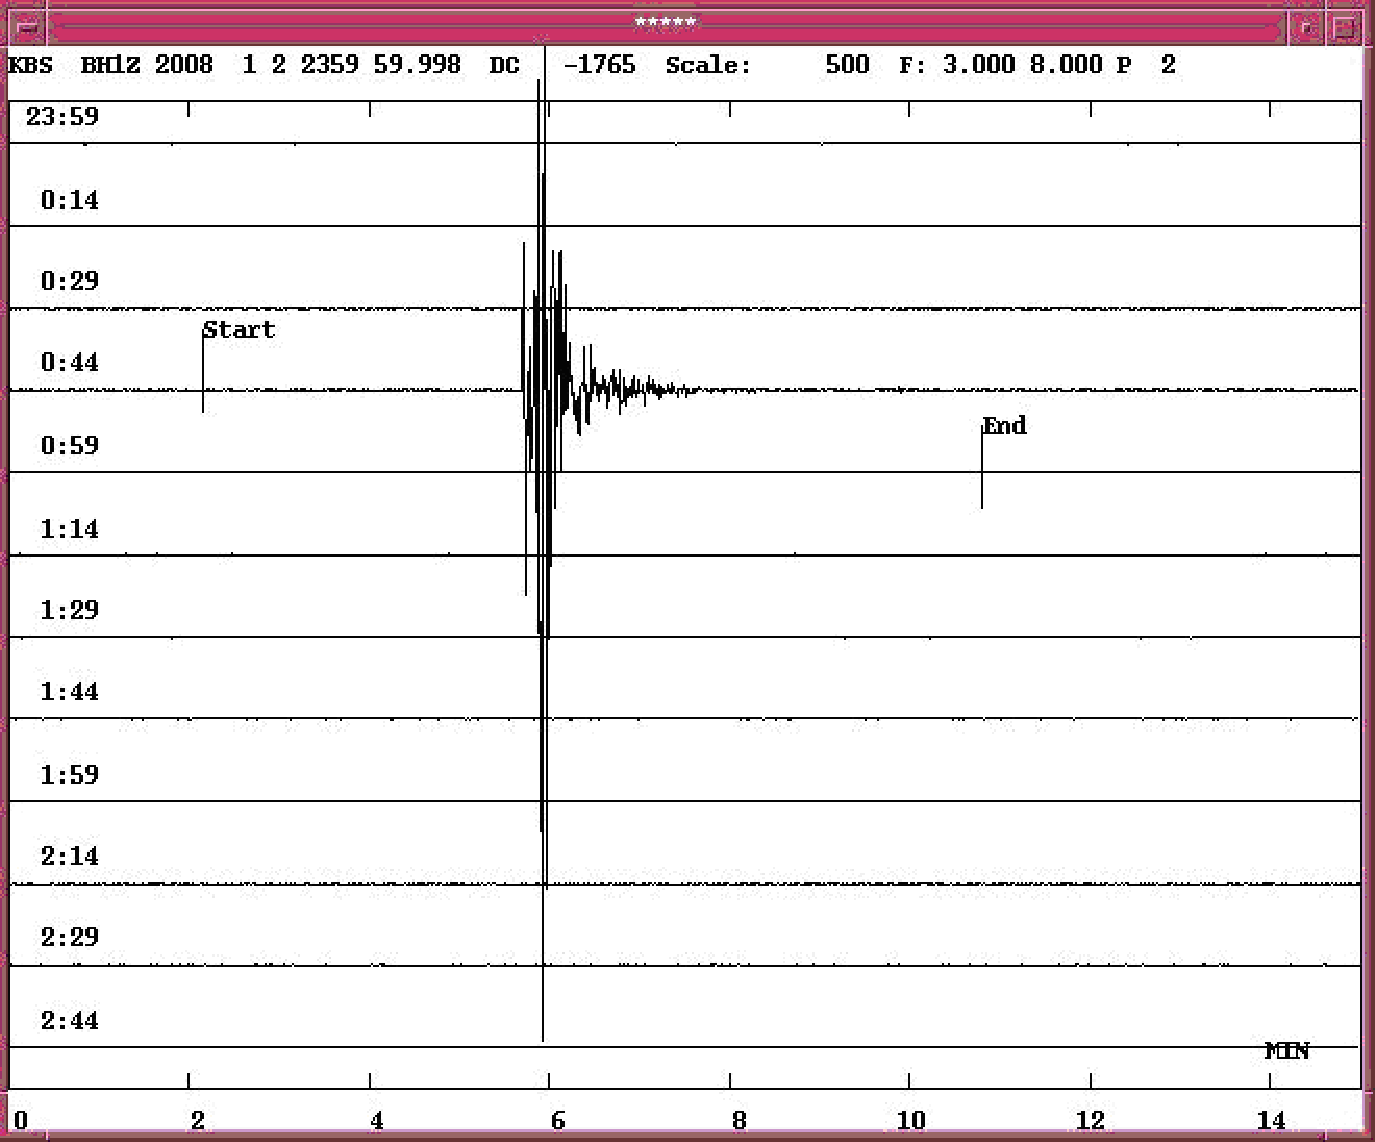
\includegraphics[width=0.9\linewidth]{fig/fig16}}
\caption{Example of time marks at the ``Start'' and ``End'' of an 
event recorded at the KBS station. The time marks is witten to the file 
\texttt{mulplt.ext} for data to be extracted and processed. Type ``s'' and ``e'' 
to add time marks.}
\label{fig:mulplt.ext}
\end{figure}

\subsection{Commands in MULPLT, overview}
\label{subs:commands-mulplt}

When the trace(s) are on the screen and the cursor is displayed, then several options are available. Most options can be displayed by pressing the MENU button in the upper right hand corner. Pressing MENU again removes the option boxes. Commands can be given by either pressing a letter or clicking on a box in the menu (Figure 
\ref{fig:mulplt-menu}
). By pressing ? or clicking on the Help button, the following help menu will be displayed: 

Help on MULPLT 

%\verbatiminput{include/mulplt.help}
\verbatiminput{include/MULPLT.HLP}

\index{Zoom in MULPLT}\index{Channel selection} \index{Filters in MULPLT}
\textbf{Filters in MULPLT}



All filters in MULPLT are Butterworth filters in time domain. When a filter is selected. using a hotkey or from the menu, the filter is only run one way, forward in time, and the number of poles is then 4. This will make a small phase delay where the first onset might appear a bit later, so if possible, read on unfiltered traces. If a 2 way filter is desired, press the filter key twice and the\index{Picking phases, use of filters} filter will also run backwards in time and the filter will be similar to an 8 poles filter. This gives theoretically a zero phase shift filter, however in practice, some of the onset energy is seen well before the first arrival, so it seems to distort the arrival times much more than using the 4 pole filter. When the program asks for a non fixed filter like when using the "." (Filt) command, the filter is always 4 poles by default. However, it is now also possible to interactively select number of poles and number of passes (1: forwards, 2: both ways)  using the ' command. Press ' and the user is asked for filter frequencies, number of poles (<10, but more then 4 and the filter might become unstable for high sample rates) and number of passes. In addition LP (low pass), HP (high pass) and BR (band reject) filters can be used. E.g for a 5-10 Hz filter some of the choices are:

\begin{verbatim}
5 10        4 pole band pass, command .
0 10        4 pole low pass, command .
10 0        4 pole high pass, command .
-5 10       4 pole band reject, command .
5 10 2      2 pole band pass, command '
\end{verbatim}
\index{Low pass filter}
\index{High pass filter}
\index{band reject filter}
\index{Filter, number of poles}
\index{Number of poles, filter}

WHEN PLOTTING, THE FILTER LIMITS, NUMBER OF POLES AND NUMBER OF PASSES IS WRITTEN ON THE SCREEN.

For band pass filters, the number of poles for both frequencies is the same. When doing spectral analysis or response removal and specifying a filter before, the filtering is done in time domain and the filter has the number of poles specified by the user, default 4. NOTE:\index{Filter and spectral analysis}When reading\index{Polarity} polarities, DO NOT USE FILTER, if possible.

Filtering and instrument correction: Since filtering is done in time domain, there is an added stability filter in frequency domain to avoid low frequency blow up. This filter is a 4 pole HP filter at 1/5 the filter low frequency corner. \index{instrument correction}

Filter limitations: For frequencies below 0.5 Hz, only 4 pole BP and BR filters can be used. If the user try to select another number of poles, the number of poles is set to 4.  

Filtered output: Extracting data with WAVETOOL, option 'Out'. It is only possible to use 4 pole BP filters, forward in time, using any other filter and the data is not filtered. Using option OutW  any filter can be used.


Prior to version 9.1
MULPLT used a 4 pole Butterworth filter in time domain and an 8 pole Butterworth filter in frequency domain. The filters in frequency domain were use in connection with instrument response correction and spectral analysis. It has turned out that the frequency domain filters distorted the signal in some cases, particularly for narrow band and low frequencies. Therefore, frequency domain filters are no longer generally used.  The change in filter setup, might change Ml magnitudes by 0.05 to 0.1 depending on which filter (if any) was used.

\begin{comment}
taken out 2012-01-27:
\textcolor{red}{pv-change: 
MULPLT uses a 4 pole Butterworth filter that can be used forward and backwards. Normally when a filter character or filter menu press is selected, the filter is only run one way and the number of poles is then 4. This will make a small phase delay where the first onset might appear a bit later, so if possible, read on unfiltered traces. If an 8-pole filter is desired, press the filter key twice and the\index{Picking phases, use of filters} filter will also run backwards. This gives theoretically a zero phase shift filter, however in practice, some of the onset energy is seen well before the first arrival, so it seems to distort the arrival times much more than using the 4 pole filter. When the program asks for a non fixed filter like when using the `.'(Filt) command, the filter is always 4 poles. When doing spectral analysis and specifying a filter before the spectral analysis, the filtering is done in frequency domain and the filter is 8 pole Butterworth. \index{Filter and spectral analysis}When reading\index{Polarity} polarities, DO NOT USE FILTER, if possible. If a filter is chosen from the menu, it is always 4 pole. 
\newline
The filter pass-band limits can be changed in \texttt{MULPLT.DEF}.\index{Change filters}. The user can also chose between two filter routines: bndpas (default) and recfil. 
\newline
The filter used in continuous mode can be either bandpass, low pass or high pass. Specifying a filter limit of zero, means that the filter is low pass or high pass. Limits of 0 10 Hz means a 10 Hz low pass filter.\index{Low pass filter}\index{High pass filter} 
}
\end{comment}

\textbf{Displaying uncertain time}

In each trace header in the SEISAN waveform file, there is a flag to indicate if the time might be uncertain (see Appendix \ref{app:seisan-format}). If that flag has been set, the message `UNCERTAIN TIME' will be displayed on top of the trace. Currently this flag is only put into the waveform files if the data comes from a SEISLOG system that has detected a timing error\index{Uncertain time}\index{Timing error} or if the data is converted from SEED/MiniSEED data. Simlarly plotting SEED/MiniSeed data, uncertain time will be displayed if that flag is set in any block in the time window read in for a particular trace. 

\begin{figure}
\htmlimage{scale=2.0}
\centerline{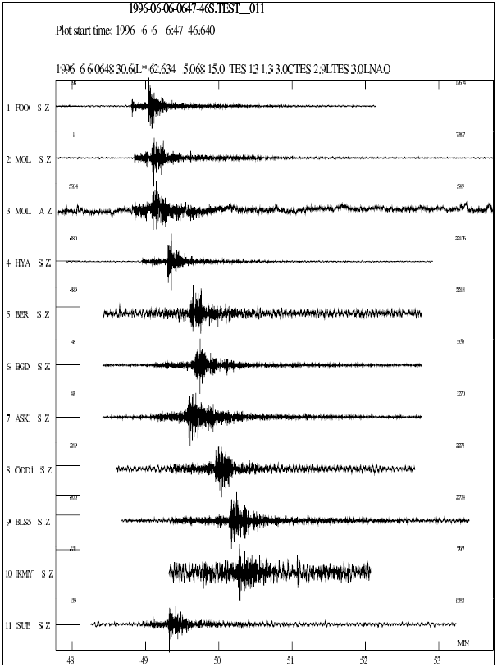
\includegraphics[width=0.9\linewidth]{fig/fig17}}
\caption{
An example of using MULPLT in multitrace plot mode. Notice that start and stop times are different for different channels. The horizontal line at the start of the plot is the \index{DC level}DC level. The small number above each trace to the right is the max absolute count with the DC-level subtracted and the small number to the left above the trace is the DC level. If plotting from EEV, the phase picks available are shown. 
}
\label{fig:mulplt-multitrace}
\end{figure}

\begin{figure}
\htmlimage{scale=2.0}
\centerline{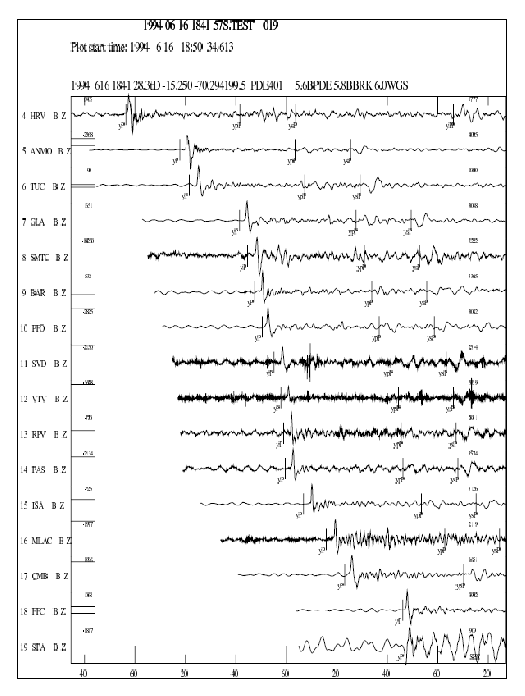
\includegraphics[width=0.9\linewidth]{fig/fig18}}
\caption{Examples of MULPLT with theoretical arrival times of some global phases. Short period seismograms are shown. The theoretical phases are marked with onset y below the trace and the read phases are marked normally above the trace. 
}
%\label{fig:mulplt-iasp}
\end{figure}

\begin{figure}
\htmlimage{scale=2.0}
\centerline{\includegraphics[width=0.9\linewidth]{fig2/fig2c}}
\caption{Example of MULPLT with theoretical arrival times showing global phases on a long period seismogram. The filter used from 0.01 to 0.1 Hz. Without filtering, almost nothing would have been seen on this broadband station. 
}
\label{fig:mulplt-iasp}
\end{figure}

\begin{figure}
\htmlimage{scale=2.0}
\centerline{\includegraphics[width=0.9\linewidth]{fig2/fig2d}}
\caption{MULPLT in continous mode.\newline
The plot shows 6 hours of long period data. The scale is 3000 counts 
between the traces and the filter used is from 0.01 to 0.1 Hz. The 
trace start time in hours and minutes is given on top of each trace. 
On the header line, P1 means the first page and DC is the DC level 
subtracted. Note that the numbers on the time scale at the bottom 
only are valid for the first trace unless all traces are 60 sec or 
60 min long.}
\label{fig:mulplt-cont}
\end{figure}

\begin{figure}
\htmlimage{scale=2.0}
\centerline{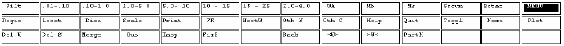
\includegraphics[width=0.9\linewidth]{fig/fig21}}
\caption{Example of the menu, which can be displayed on top of the plot.
}
\label{fig:mulplt-menu}
\end{figure}

Below is some more detailed description of some of the options. The one letter command is given 
with the menu command in parenthesis: 

To apply filters, first make a selection of options (filter, window, channel selection) and then execute by pressing R(Plot) (or selecting a zoom window). Figure 
\ref{fig:mulplt-multitrace}
shows an example. 

\index{Phase picking mode}Single trace mode: \index{Single trace mode}

In this mode, one trace is initially displayed on top of the screen, see example on Figure 
\ref{fig:mulplt-pick}.
The traces used are the ones earlier selected and will be displayed one by one. Several options are now possible as can be seen on the menu. Normally no hardcopies are made in single trace mode\index{Hardcopy in single trace mode} since it is intended for fast routine work. However, by starting MULPLT in multitrace mode (option 2) and then go to single trace mode (command T(Toggl)), hard copy files are made. 

Multitrace mode: 

In this mode hard copies can be made. If option 2 is used, both screen plot and hard copy files are made. If replot is made, only the last plot is available in the hard copy file. If option 3 is used, which is only hardcopy, there will be additional questions about, window length, start time, scaling and filters. If the scaling is set so that the plot occupies more than one page, several pages will be printed. If in this mode, \texttt{filenr.lis} is given as file name, the program assumes that all the files should be plotted and the only questions will be about the scaling and filters. All channels in each file will be plotted. This option is useful for plotting a large number of events with a single command. 

All channel mode\newline
In this mode, all channels for selected stations are displayed in a new window. This mode is particularly useful for working with three component data. By selecting one or several stations in multrace mode, all components for those stations will be displayed in new window by pressing y or ALLC on menu. Similarly in single trace mode, prsssing y or ALLC will display all channels for that station. The user can then go back to e.g. multitrace window and select another station to work with in three component mode.
\index{All channel mode} \index{Three component plotting}

Multiple screens in multitrace mode 

If many channels are available (like more than 30), it might be difficult to distinguish all and the channels can be displayed in multiple screens. The number of channels per screen is set in \texttt{MULPLT.DEF}. The number of windows or screens for a particular data set is given in top left hand corner as e.g. `Win 2 of 7' meaning current window is number 2 of 7 windows. To move to the next window, use TAB or NextW in menu. In each window, normal operation can be done. Channels selected will be kept. Using a large data set, the user can then view each window separately, select the channels of interest and when all channels have been viewed, only the selected channels will remain for display.
It is possible to togle between showing all channels and multiple screens by pressing N.  


Plotting stations in a given distance range
\index{MULPLT, plotting station in a max distance}
\index{Distance range, plotting}
When many stations are available, it might be useful to only plot only the stations nearest the epicenter or a particular location. For this option to work, parameter MULPLT AREA in  MULPLT.DEF must be set to a value larger than 0.0.  Then only channels with a distance ( radius degrees) larger than a given value from a point (midpoint) will be selected for plotting. The options for MULPLT AREA are:

1: midpoint from epicenter in S-file, radius from MULPLT.DEF
2: --------------------, ---------------------------- interactive
3: midpoint and radius from MULPLT.DEF
4: midpoint from MULPLT.DEF, radius interactive
5: midpoint and radius interactive

If interactive options are selected, the question(s) will come out just before plotting. Once a plot is made, the radius can also be changed interactively by using command R in multitrace mode. After selecting a new radius, the channel selection screen will come up with the channels selected. This option is not dependent on stations already being present in the S-file since all station information is taken from the STATIONx.HYP file.



\index{Channel order}Channel order in multitrace mode: 

Normally channels are plotted in alphabetical order according to station name, see parameter CHANNEL SORTING in \texttt{MULPLT.DEF}. They can also be plotted in the order they are stored in the waveform file(s) (option NSORT\_DISTANCE set in \texttt{MULPLT.DEF}). By setting the channel order parameter in the \index{MULPLT.DEF}\texttt{MULPLT.DEF} file, it is also possible to plot the channels in distance or time order. If MULPLT is started from EEV (and distance ordering is set), the channels will be plotted 
%\textcolor{red}{jh-change: 
in distance order provided distances are given in file. 
\index{Distance order}. 
Since there is no consideration for channels for the same station, the channels for one station, will be plotted in the same order as given in the waveform file. If a station is not found in the S-file, it will be plotted last. If plotting is done with MULPLT directly with a waveform file, the plotting order will be the start times as given in the waveform file header. Channel ordering can be turned on with the key "-" or pressing (Dist). If set in the \texttt{MULPLT.DEF} file, it 
is set when MULPLT starts up. It cannot be turned off for a given event when set from MULPLT but the flag is returned to the default value for the next event. 

Plotting from continuous data base 
\index{Continuous data}\index{Plotting continuous data} 

If a continuous data base is set up (see section \ref{subs:cont-data}), it is then possible to plot all traces from the continuous data base with MULPLT. \index{Cont}\index{Mulplt, option cont}When MULPLT starts up, use option cont and the user is prompted for a start time and interval. MULPLT will now check all continuous data bases for available data in required interval and display the available data. The forward (next) or back option will display previous or next window respectively. There is an 25 \% overlap between windows. If no data is available for the whole window, no trace is shown. If the beginning and the end is available, a line will join the two segments. If only end or beginning is available, only the available data is shown. All normal operation can be done on the window plotted so it is possible to e.g. extract data. If the register option is used, the whole window is extracted from the continuous data base as one file, copied to WAV and the S-file created. 

\subsection{Registering new events into SEISAN}
\index{New events into SEISAN}

Mulplt is the main tool for checking and putting new events into SEISAN. New events with waveform data can appear in two ways in SEISAN: 

\begin{enumerate}
\item
 Unprocessed waveform files are available in a work directory and have to be inspected and possibly put into the database. No S-files have been made. 
\item
 Raw data has already been put into a SEISAN database with S-files and corresponding waveform files in some work directory, the data has not been checked. This process has most likely been done with the automatic data collection software SEISNET \citep{ottemoller1999}, however, events can also have been auto registered with program AUTOREG.
\item 

Registering from continuous data: SEISAN continuous data base, BUS or SeisComp archives or a large SEED file.

\end{enumerate}

In both cases above, the aim is to inspect an event and decide if the event is real and should be put into the database using option `p'. All work must be done from the directory where the raw waveform files are located. The process of putting an event into the database results in creating the S-file (option1), giving the event identifiers and copying the waveform files of registered events to the waveform directory.By pushing p(Regis), the user will be prompted for \index{Distance indicator}distance indicator, which has to be L, R or D for local, regional or distant event. It is possible here to enter 2 characters like LE or LV for local explosion or local volcanic event. The \index{Event type}event type or \index{Event ID}event ID can be any character. Four characters are predefined and should only be used if the following definition correspond: P(probable explos\index{Explosion}\index{Volcanic event}ion), E(explosion), Q(confirmed earthquake) or V(Volcanic event). If the user enter L, R or D in lower case, the case will automatically be changed to upper case. The same also happends with E, P, Q and V. A third cahracter can optionally be entered for the model indcator \index{Model indicator}  which is put into column 21 of the header line. The volcanic events have a sub classification which can be entered when registering an event as volcanic, see section \ref{sect:volcanic}. The process of registering the event into the database implies that a new S-file is created or registered and in the S-file. An operator ID will be asked and the operator ID will be put on the \index{ID-line}ID-line. The question about operator will only be asked for the first event since it is assumed that all subsequent events are put into the same database by the same operator. The event ID, can later be used with the SELECT program to select out particular event types. When first putting an event into the database, the user is also prompted for database.  

Option (1) \newline
Data is available as waveform files only and a list of files must be 
made first with DIRF. Main option 0, 1 or 2 can be used for plotting. 
The `p' option creates the S-file and copies the waveform file to 
the WAV directory. The waveform file remains in the working directory. 
Unwanted waveform files can also be deleted so that when all events 
have been put in, only waveform files of `real' events remain in working 
directory. These can then be plotted with one run of MULPLT, see 
section \ref{subs:mulplt-main}.  

Option (2) \newline
Data is available already in a database, however since the data has not been inspected, the waveform files are still in a work directory. In EEV, the first unprocessed event in the month is found 
with command `ss' and MULPLT is started with command `po' to invoke all defaults. If the event is to remain in the database, it must be registered with option `p'. The process and the questions are the same as in option (1) except that the S-file is not created since it is already there. The S-file is cleaned for all processing information from SEISNET\index{SEISNET}\index{Delete S-file}\index{Delete waveform file} if present. This normally also includes automatic phase picks. However, they can be kept if parameter REG\_KEEP\_AUTO is set in the \texttt{SEISAN.DEF} file. \index{REG\_KEEP\_AUTO}\index{Delete automatic picks}The status of the files also changes to being newly registered as under option (1) (see definition of processing codes in Appendix 1) and waveform file(s) copied to WAV. Before registering, it might be an advantage to merge waveform files and delete unwanted files (could be false triggers), see section \ref{subs:commands-mulplt}. Files can only be merged and deleted in working directory with commands Delw and Merge (Menu). In this process of putting new events into the database, it is also an advantage to delete unwanted events. This is done with option `S'(Del S)'. The S-file is deleted, but the waveform files remain in the working directory. 

Option (3) \newline

When reading continuous data, an output file can be made with the Out option and that output file can be registered. However, it is also possible to do this in a single operation using the Register option like above. The selected time window is then extracted, the waveform file copied to WAV and the S-file registration made. In addition to the questions above, one additional question is given: 

Output channels on screen (s) or all channels(enter)

This option is intended to be used with routine operation when many channels are present and the user only views a few, like all vertical channels, but want to extract (and register a file with all channels).

\index{Preprocessing of data}Preprocessing of data while registering new events, option (1) 

Normally a series of events are registered first and MULPLT terminated. Then EEV is started up for interactive picking and location. However, if preliminary processing is desired while registering the event, this is also possible. 

\index{Registration and preprocessing}Phase picks:If phases are picked before the event is registered, these readings are saved in the database at the time of registration. After the event has been registered, MULPLT automatically goes to the next event in FILENR.LIS and no more phase picking can be done. 

Processing with a given program: 
Optionally MULPLT can, after registration, start any program processing the newly registered event. 
E.g. the AUTOPIC program can be started or a program reading amplitudes etc. The program name is defined in \texttt{MULPLT.DEF}. 

Locating the event: As the final step after registration, the event 
can optionally be located and the location optionally placed in the 
database. \newline
The above options have been put in on the suggestion of Brian Baptie, who is using it for rapid processing of volcanic events, where in most cases the operator only wants to look at the event once. 

\subsection{Adding BUD archive waveform data to nordic file, WAV2BUD}
\index{Adding BUD archive to nordic file}
\label{page:wav2bud}


The program WAV2BUD reads nordic files like \texttt{collect.out} or 
\texttt{select.out} and add lines (type 6) to each event in the input file 
that link to the waveform data in a BUD archive.
Note, it is only the data given in \texttt{SEISAN.DEF} by the 
ARC\_CHAN parameter that are linked to. The events with the 
new data link is listed in the \texttt{budfile.out} file.\newline
The program is written by \textbf{Ruben Soares Lu\'is}.

\subsection{Phase picking, amplitude, weight and polarity}
\index{Phase picking}

Picking phases: 

The plot will display any pick present in the database (current S-file). To pick new phases, position cursor at phase, and press the key as indicated on top of the screen (if in Single mode). E.g. pressing 1 will read IP. Pressing the same key again with the cursor at a different place will delete the old one (indicated with a D) and display the new one. Additional default phases, which can be picked, are i for I, e for E and A for AMP (note upper or lower case). Keys for phases have default definitions, but can be redefined using the file \texttt{MULPLT.DEF}, see below. The end of the coda is picked as a phase (C) and the program calculates \index{Coda length}coda length IF AND ONLY IF A P-READING IS PRESENT. 

Picking amplitudes: 

Position the cursor at the bottom or top of a wave and press a, then at the other extreme (bottom or top) and press a (do not use upper case, see below). There is no requirement for going left to right or top to bottom, it can be done in any order as long as the two extremes are marked. At each press, a cross is marking where the pick was made. In case a filter, like WA, MS or Mb is applied, the program will associate the amplitude with the respective amplitude reading (AML, AMS or Amb). \index{Phase AMP}\index{AMP} Amplitude and period are calculated and stored with the phase. Otherwise, if none of these filters are applied, a menu pops up and the user needs to select a phase name to which the amplitude and period readings are associated. It is often a good idea to store amplitudes with the nondescript phase E, I or AMP since it then will remain even if the phase is deleted or changed. If an attempt is made to pick amplitude on a trace which is not in nm, the reading must be confirmed since SEISAN assumes all amplitudes to be in nm (see section on instrument correction). If no phase is picked, no amplitude is stored. The amplitudes are always assumed to come in pairs so if 
e.g. 3 amplitude values have been picked, and the user tries to pick a phase or quit the program, it will appear frozen since the program is still waiting for the next amplitude measurement. It is always the last pair of amplitude measurements, which are used. Amplitudes can be picked on both corrected and uncorrected traces.\index{Problem, picking amplitude} 

If A is pressed instead of a, the amplitude is read and marked automatically. It works in most cases, but sometimes two subsequent peaks are not correctly chosen and the amplitude reading has to be done manually. The method is to find the absolute extreme and then the largest amplitude before or after is selected in order to obtain the peak to peak amplitude, from which the amplitude is calculated by dividing by 2. For more information, see.  ../LIB/auto\_amp.for.\index{Amplitude, automatic}\index{Automatic amplitude} 

\index{Component names in S-file}Component names when picking phases: 

In the S-file, the component only has 2 letters while in the waveform file it has 4 letters. There must therefore be a unique translation between the two. This definition is given in the subroutine componen.for\index{Componen.for} in LIB. Most common combinations are now defined, however if a new one is defined in the waveform file which does not exist in componen.for, the first and last letter of the input component will be used. If e.g. an input component is called SS Z, then the code in the S-file will be SZ. This means that picks for stations with components, which do not differ in first and last character, cannot be separated in the S-file. Component names for rotated channels will be e.g. SR and ST for short period radial and transverse components respectively. 

Reading \index{Polarity}polarity: 

If the cursor is above or below the trace at a distance marked by horizontal tics on the sides of the plot, the first motion is also picked and displayed. Do not use a filter if possible.  
Assigning w\index{Weight}eight: 

A phase can be assigned a weight. Move the cursor close to a pick and press one of the keys 1-9 in \index{UPPER case}UPPER case thus using e.g. !"\# (default, can also be changed), and a \index{HYPO style weight}HYPO style weight is assigned and displayed. Although weights 0 to 9 can be put in, HYP only uses 0-4 and 9 (see section \ref{subs:hypocenter-program}). Phases with associated \index{Amplitude}amplitude, \index{Period}period, \index{Azimuth}azimuth or \index{Apparent velocity}apparent velocity are displayed with a hat below on the phase indicator line. The default keys for the weights might not be correct on all keyboards, if not, set keys in \texttt{MULPLT.DEF}.  

Automatic determination of coda length\index{Automatic coda length}\index{Coda length} (C or c): 

The coda length can be quite variable among different operators and a function has been made to automatically determine the coda length. The signal is bandpass filtered and the end of the coda is determined by a standard STA/LTA procedure. The parameters are set in the \texttt{MULPLT.DEF} file. Press C to find coda length automatically or c to determine manually. If parameter CODA AUTO is set in \texttt{MULPLT.DEF}, c I sused. The coda length can only be determined if a P-phase is present. 

\subsection{Theoretical arrival times for global and local phases and location}
\index{Global phases} 

In order to assist in \index{Identifying seismic phases}identifying seismic phases, there is an option for displaying the theoretical arrival times of several global and regional phases while picking phases. The steps to do so are the following: 


\begin{itemize}
\item[1]
 Before entering MULPLT from EEV, the theoretical travel times have to be calculated for the current event. This assumes that the origin time and hypocenter is given in the header line or a subsequent type one line. If not, enter manually (from e.g. PDE) or use the EEV command INP\index{INPUTEPI}UTEPI or IN\index{INPUTONE.}PUTONE. Then proceed to calculate the theoretical arrival times using EEV command IASP with the \index{IASPEI91}IASPEI91 traveltime tables (for more details, see section \ref{subs:iasp}). The same command is also available inside MULPLT in multitrace mode. All arrival times (or a subset, see \ref{subs:iasp}) for all stations in current S-file will now be calculated with program IASP and stored in file iasp.out (no importance for the use, just for information). See Figure 
\label{fig:mulplt-multitrace}
for an example in multitrace mode. Note that very many theoretical phases can be generated if the S-file has many stations. MULPLT will stop if more phases are used than the di\index{Dimension}mensions are set up for (include file seidim.inc), and you must use fewer phases (a warning is given when 500 phases are generated) or set up SEISAN with larger dimensions, see section 3. Theoretical local crustal phases for the current model can  be calculated with program WKBJ and displayed, see section \ref{sect:synt-seismogram}. Theoretical phases can also be calculated when using the location option, see next section. 

\item[2]
 Pick phases: When a trace is displayed on the screen, all theoretical phases inside the time window will also be shown. To distinguish the \index{Theoretical phases}theoretical phases, they are prefixed with a y and displayed below the trace (normal phases have I, E or blank and are displayed above the trace). Position cursor where you see a phase which you think corresponds to a theoretical phase and press y. The nearest theoretical phase will now be placed at that position with a prefix E. Only theoretical phases selected in this way will be written in the S-file. Note that the phase names can be up to 8 characters long, see Appendix 1 for the definition of \index{Long phase names}long \index{Phase name}phase names. 
\end{itemize}

If the phases fit badly, start looking at the P-phase. If that does not fit the theoretical P-phase, change the origin time in the S-file so that the P-arrival fits, and recalculate the theoretical phases.  

PROBLEM: In multitrace mode, only one theoretical phase can be picked. Replot must be made before picking the next. \index{Problem, reading synthetic phase}

Locate earthquake \index{Locate event in MULPLT}

If several phases have been read and saved in the S-file, the event can, in multitrace mode, be located with command l (Locat), just as in EEV. The screen is cleared and the usual location rolls over the screen. When the location is finished, the plot will reappear and the calculated travel times will be displayed as synthetic phases (see previous section). In this way it is possible to immediately visualize the differences between the read and calculated phases. The output files are \texttt{hyp.out} and \texttt{print.out} as usual. 

\subsection{Instrument correction and magnitudes Ml, mb and Ms}
\index{Ground motion seismogram}

The correction for instrument response is done by taking the spectrum of the selected window of the trace, dividing with the response function and converting back to the time domain. Any filtering specified is done in the frequency domain. Filtering is needed in most cases. 

Ground motion 

Option g(Groun) removes the effect of the instrument and displays a ground motion seismogram. After selecting g and the zoom window, there is a question of which type of seismogram to calculate: \index{Displacement}Displacement (d), V\index{Velocity}elocity (v) or \index{Acceleration}Acceleration (a). The corrected trace is shown below in \index{Nanometer}nanometers(nm), nm/sec or nm/(sec*sec) (if \index{Response file}response information is available). Note that this might produce strange seismograms, since e.g. a SP seismograph has very low gain at low frequencies so noise might be amplified very strongly. It is therefore recommended to also do some filtering when using the g option. 

Amplitude for determining Ml 

For the w(WA)-option \index{Wood Anderson}(Wood Anderson), the trace is corrected for the instrument to produce displacement. The displacement trace is then multiplied with the response of the Wood-Anderson instrument to produce a signal to look exactly like it would have been seen on a Wood-Anderson seismograph. The maximum amplitude (nm) is read and saved to the S-file with name IAML. The Wood-Anderson response (PAZ) is hardwired in SEISAN and it is similar to a 2 pole Butterworth high-pass filter at 3 Hz.   In SEISAN versions prior to 8.3, a fixed 8 pole bandpass filter was used (1.25 Hz - 20 Hz). Filtering is done in the frequency domain. For noisy traces it might also be required to put a filter at the high end. This can be specified in the \texttt{MULPLT.DEF} file. Unfortunately, the correct low cut filter with 2 poles will often result in the seismogram blowing up at low frequencies and might be quite useless for earthquakes with magnitude below 2.0 - 2.5  So in addition to the PAZ filter, a fixed bandpass filter can be added (see \texttt{MULPLT.DEF}). In the standard distribution of SEISAN, this additional filter is set to an 8 pole filter at  1.25 - 20 Hz. In all cases where an additional filter is used, the read amplitude is corrected for the filter gain and the true ground motion written in the S-file will be larger than the amplitude seen on the screen. The additional default filter probably only makes a difference for very large events (Ml $>$ 5). Other filters at a higher frequency should only be used for small events (M$<$1) .  NOTE: In SEISAN version 7.1.1 and earlier, the low cut filter was set by mistake to 0.8 Hz. Repicking amplitudes with the correct filter might change magnitudes of larger events slightly.

Displaying response information 

The response function for the current channel can be shown with option `:' (Resp), see Figure 
\ref{fig:mulplt-resp}.
If no response function is given, a message is shown. If the response function is taken from the waveform file header instead of from the CAL directory, a message is given. \index{Response, from where}\index{Response, show curves} 


Amplitude for determining \index{mb}mb: 

Determining mb assumes that the maximum amplitudes are measured on classical 1 Hz WWSSN instruments having a peak gain around 1.5 Hz. This in reality means a band limited measurement.  To pick ground amplitudes for determining Mb on instruments with a broader or more narrow frequency band, like most high frequency SP instruments, some filtering must first be done. Using the j(mb)-option, the trace is corrected for the instrument to produce displacement. The displacement trace is then multiplied with the response of the SP WWSSN instrument to produce a signal to look exactly like it would have been seen on a SP WWSSN seismograph. The unit of the amplitudes seen on the screen is nm, however the amplitude will only represent the ground motion correctly at the frequency of the maximum gain at 1.5 Hz and for all other frequencies, the true ground motion will be larger than seen on the screen. The maximum amplitude is now picked and displayed below the trace, corrected for the gain relative to the gain at 1.5 Hz and written to the S-file with name IAmb. This means that the amplitude written to the S-file generally will be larger than the amplitude displayed on the plot. The SP WWSSN response (PAZ) is hardwired in SEISAN and cannot be modified with filters.

In SEISAN version to 8.2.1, the default filters used to simulate SP WWSSN were, by mistake, in the band 0.9 (2 pole) to 1.8 Hz (3 poles). This will result in slightly wrong magnitudes unless the user had put in correct new filter contants... Prior to SEISAN version 8.2, the default filters used were 0.5 Hz (8 pole)  and  5.0 Hz (8 pole filter), which was close to the correct values. No correction for relative gain was used in SEISAN versions prior to 8.3.. All of these changes could have resulted in smaller errors in mb, which only can be corrected by repicking the amplitudes.

Amplitude for determining mB

Amplitude for mB is defined as the maximum velocity on a wide band instrument (0.2 -30 sec or 0.033 - 5 Hz). The maximum amplitude Vmax is measured on a velocity trace. Using the J(mB) option, a velocity trace (nm/s) in the frequency band 0.033 - 5 Hz is displayed. The maximum amplitude in nm/s (irrespective of frequency) is picked and displayed below the trace. This amplitude is now written to the S-file with phase name IVmB\_BB. In principle, mB can be calculated using any instrument, but in practice it can only be used if the P-signal is seen clearly on an unfiltered broad band velocity record.
The Butterworth filter 0.033 - 5 Hz , 8 poles, is hardwired and it cannot be modified with additional filters.

Amplitude for determining \index{Ms}Ms: 

The attenuation function for determining Ms assumes that the amplitudes are measured on classical LP WWSSN instruments having a peak gain around 15 second. To pick ground amplitudes for determining Ms on instruments with a broader or more narrow frequency band, like most broad band instruments, some filtering must first be done. Using the k(Ms)-option, the trace is corrected for the instrument to produce displacement. The displacement trace is then multiplied with the response of the LP WWSSN instrument to produce a signal to look exactly like it would have been seen on a LP WWSSN seismograph. The unit of the amplitudes seen on the screen is nm, however the amplitude will only represent the ground motion correctly at the frequency of the maximum gain at 15 seconds  and for all other periods, the true ground motion will be larger than seen on the screen. The maximum amplitude is now picked and displayed below the trace. This amplitude is then corrected for the gain relative to the gain at 15 seconds and written to the S-file with name IAMs\_20. This means that the amplitude written to the S-file generally will be larger than the amplitude displayed on the plot. The LP WWSSN response (PAZ) is hardwired in SEISAN and no additional filters can be used.

The attenuation function for determining Ms assumes that the amplitudes are measured in the period range 18 - 22 sec and it is up to the user to make sure that the the amplitude is in the correct range.. 

For SEISAN 8.2.1, the default filters used were in the band 0.038 (2 pole) to 0.1 Hz (1 pole). Prior to SEISAN 8.2 default filters were 0.042 to 0.063 Hz (8 pole filter). No correction for relative gain was used in SEISAN versions prior to 8.3. These changes might have resulted in small errors ins Ms and can only be corrected by repicking the amplitudes.

Amplitude for determining MS

Amplitude for MS is defined as the maximum velocity on a wide band instrument (3 -60 sec or 0.017 - 0.3 Hz). Using the K(MS) option, a velocity trace (nm/s) in the frequency band 0.017 - 0.3 Hz is displayed. The maximum amplitude in nm/s (irrespective of frequency) is picked and displayed below the trace and written to the S-file with phase name IVMs\_BB. In principle, MS can be calculated using any instrument, but in practice it can only be used if the surface wave is seen clearly on an unfiltered broad band velocity record. The big advantage with using MS is to avoid the 18-22 s limitation needed for Ms. The Butterworth filter 0.017 - 0.3 Hz , 8 poles, is hardwired and cannot be modified with additional filters.

Problem: If a long trace (large number of samples) is used, the instrument correction might fail (funny result seen) due to numerical overflow in the spectral conversion. Choose a shorter window. \index{Problem, instrument correction} 

\subsection{Determine azimuth of arrival (3 comp or array) and component rotation}

Azimuth of arrival from \index{3-component stations}3-component stations, h(Azim) 

If a 3 component station is available, the azimuth of arrival can 
be determined using the method developed by \citet{roberts1989}. 
Display any of the 3 components and press h (Azim). Then select a 
zoom window around the P-arrival of a few secs duration for the 
analysis. The 3 components will now be displayed below in order Z, 
N and E and the calculated azimuth, apparent velocity and correlation 
will be displayed at the bottom line. In order to check the stability 
of the estimate, try different windows and filters. Often, a filter 
must be used to get reliable results. The displayed azimuth and 
apparent velocity is only saved in the S-file when an associated 
phase is picked. THAT PHASE MUST BE PICKED ON THE SINGLE UPPER 
TRACE SEEN ON THE SAME SCREEN. If there is none, use I or E. The 
velocity estimate is not very reliable and is dependent on the local 
velocities. In order to calculate the apparent velocity, the P-velocity 
of the top layer must be given. The default value is 5.0 km/sec, but 
another value can be set in the \texttt{MULPLT.DEF} file. To get a 
good estimate, the correlation coefficient should be as high as possible 
and positive. The quality of the obtained azimuth can be tested by 
locating the event with the calculated azimuth weighted out and observe the azimuth residual. 
Figure \ref{fig:mulplt-3comp}
shows an example.

Azimuth and apparent velocity from array data, FK analysis\index{FK analysis}\index{Apparent velocity} f(FK) 

Using this command, the traces seen on the screen will be put into the FK program and an FK plot will be displayed. The azimuth and apparent velocity with the highest correlation is selected by the program, however any other value can be manually selected. The values will ONLY enter the S-file if associated with a phase in the same way as amplitudes are picked. For more details, see section \ref{sect:fk-analysis}.
% 6.29. 

\index{Rotated seismograms}Rotated seismograms 

Option u(Rotat) will rotate the \index{Horizontal component}horizontal components for the next plot if the two horizontal components are available. The rotation will display the radial component instead of the N-component and the transverse component instead of the E-component. The back-azimuth used is displayed above the trace. All channels will be displayed  rotated until u(Rotat) is pressed again This means that phases can be picked and spectra made with the rotated channel. When picking phases on rotated signals, these will appear in the S-file with components R or T instead of N and E respectively. This also means that only if the rotated signals are shown, will the phases read on rotated channels appear on the plot. The station b\index{Backazimuth}ack-azimuth is obtained in the following way: If a hypocenter is given in the header line, the angles are calculated using the current \texttt{STATIONx.HYP} file. If no hypocenter is available, the angle will be read from the S-file under column observed azimuth (47-51) (if not blank) and the azimuth residual will be added. This option permits the user to first determine the azimuth with the 3-component option and then rotate the signals with the determined azimuth. Finally, if no observed azimuth is available, the event to \index{Station azimuth}station azimuth + 180 deg. will be used if available (column 77-79). If no back-azimuth\index{Backazimuth} can be found, no rotation is done and an angle of 999 deg. is displayed. If in single trace mode and choosing the 3-component option AND the rotate option, the user will be prompted for a rotation angle and the rotated channels will be shown in the usual 3-component plot, however, the azimuth determined is done with the unrotated channels. 

\index{Problem, Rotation and removing response}PROBLEM: In general, the R-channel will use the response of the N-channel and the T-channel will use the response of the E-channel so for instrument response removal to be correct, the 2 channels must have the same response curve. 

\subsection{Data manipulation commands}

Select other channels: o(Oth) 

The channel selection menu comes up again. 

Go back one channel in single trace mode, go back one event in multitrace mode if MULPLT is started from EEV: B(Back) 

Select other waveform files from S-file: W(OthW) 

If more than one waveform file available for the event, one or several others  can be selected. 

Delete waveform files: 

This can only be done in multitrace mode: The command is d(DelW) and the cursor must be above the top frame of the plot. There are two possibilities: 
\begin{itemize}
\item[1]
Input is from \texttt{filenr.lis}: The current file is deleted and if in default mode, the plot moves on to the next event.\index{Waveform file, delete}\index{Delete waveform file} 

\item[2]
 MULPLT is started from EEV: If only one waveform file is available, the program proceeds as under (1). The waveform file is deleted and the waveform file entry in the S-file remains. However, if more than one waveform file is available, the user can use a menu to select which files to delete. Only the waveform file entries in the S-file are deleted, the waveform files remain. This option is mostly used with SEISNET. 
\end{itemize}

Delete S-files D(Del S) 

This command deletes the current S-file. It can only be used if MULPLT is called from EEV. No waveform files are deleted. 

Merge waveform files given in S-file M(Merge) 

The files will be merged\index{Merge waveform files}\index{Waveform files, merge} to one waveform file and the old individual file names removed from the S-file and replaced by the new file name of the merged file. The original waveform files remain. Files to be merged will be shown on a menu. Mostly used with SEISNET. The user MUST have files in working directory. If files are in the data base, they will not be shown on the merge menu. 

% jens
Overlay two channels: It is sometimes practical to be able to overlay 2 or more 
channels. The channels to be overlaid must follow each other on the screen (sorting might influence that). Move the cursor to the channel name of the lower of the two channels, press \& and the channel is marked with a cross. When doing replot, that channel will be plotted in red on top of channel above. Both channels will be autoscaled, but if absolute scaling is used, the real difference in amplitude is seen. Overlay cannot be deselected without leaving MULPLT. This option is particularly useful when comparing real and synthetic seismograms result form moment tensor inversion, see that section later. \index{Overlay channels in MULPLT}

Output of binary waveform file, O(Out) 

It is often useful to be able to select  part of a waveform file and save it. The Out option makes an output file of the traces AS DISPLAYED ON THE SCREEN with exactly the same channels, \index{Extract from waveform file}\index{Waveform file, extract from}and time window in a file with a standard SEISAN waveform name. The output format is alw\index{MERGE\_WAVEFORM}ays SEISAN, even if some input files have a different format. The network code in the file name will ALWAYS be the station code if all channels are from the same station  Otherwise the network code has the default name MERGE. Alternatively the parameter MERGE\_WAVEFORM can be set in \texttt{SEISAN.DEF}. The data is output exactly as displayed on the last screen, so if filtering or instrument response has been made, the output file will also be filtered or instrument corrected WITH SOME RESTRICTIONS: Not all response, channel or filter combinations are possible. Only 4 pole band pass filters can be used, no rotated channels and none of the magnitude simulated traces like Wood Anderson for Ml. if you want exactly what is seen on the screen for all combinations, use option \texttt{OutW}.  If any filtering or instrument response correction has been done, a note will be inserted in the SEISAN waveform header so the user can see that this is no longer the original data. The note could be e.g. ` Displacement 1.250- 20.0 Hz' indicating that output has been filtered and converted to displacement (nm). Note that numbers have been scaled so only if the SEISAN file is read with standard SEISAN routines, will the numbers be correct. If the output file is converted to ASCII by SEIASC, the number shown must be multiplied with a given scaling factor, see SEISAN binary format description (Appendix \ref{app:seisan-format}). There is no response information in the header other than the short text. Since the station code is still the same, it is technically possible to correct for the response again using the response information in the CAL directory, 
\textbf{however, be aware that this will give wrong results}.

Option \texttt{OutW}:This option will output the signal exactly as seen on the screen with all the selected filter and response combinations. It also handles rotated channels. The output file is \texttt{mulplt.wav} and it is an Ascci file with real numbers in Helmberger format (readable by SEISAN). To make the file, press \texttt{OutW} and wait for message '\texttt{mulplt.wav written}' in top right of the screen. For many channels and high sample rate it could take some time since the output is Ascii. If the traces in the window do not start and stop and stop at the ends, then dc levels will be added so all channels in the output file has same start and stop timers. Format description is found in section moment tensor inversion. \index{mulplt.wav} 

Output of ASCII waveform file 

This option only works if parameter SPECTRAL\_OUTPUT has been set in \texttt{MULPLT.DEF}. The output file signal.out contains the last data displayed in the single trace zoom window (in ASCII and real numbers). This option is a another way (see option O(Out) above) of getting an output file that has been filtered or instrument response corrected.  The main difference is that this file is only for one trace \index{Signal.out}\index{Extract data in MULPLT}\index{Output, corrected trace}written in ASCII. 

\index{Fixed scaling}Fixed scaling 

Normally all traces are plotted with au\index{Autoscaling}toscaling. However, it is sometimes useful to be able to scale the traces with a fixed scale in order to e.g. compare traces or override the autoscale in case a spike distorts the autoscaling. Option *(Scale) will prompt the user for a maximum count to use for the scaling of all traces. 

\begin{figure}
\htmlimage{scale=2.0}
\centerline{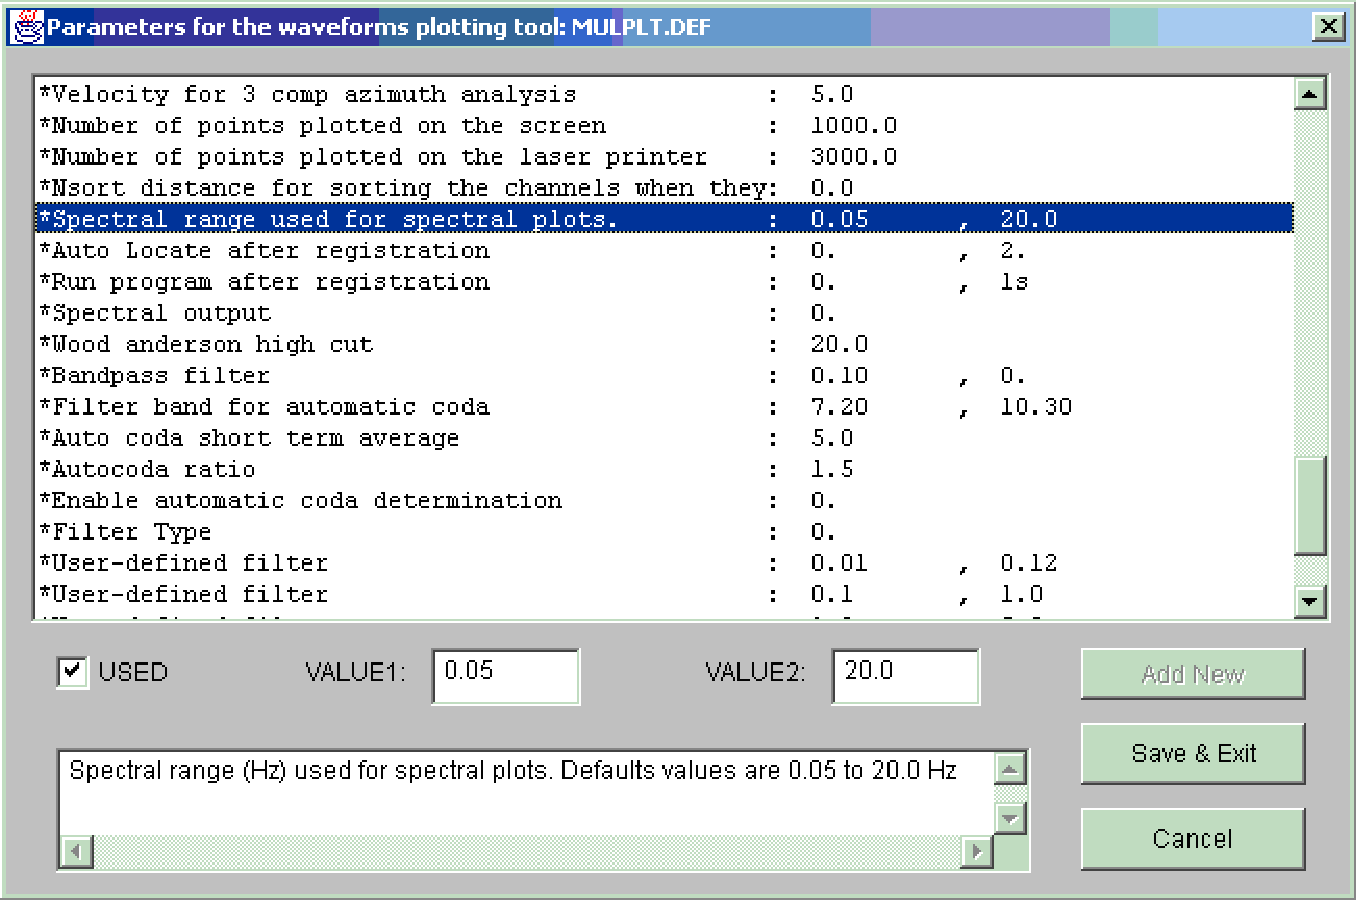
\includegraphics[width=0.9\linewidth]{fig2/fig3}}
\caption{Using MULPLT for picking phases. The top shows the original trace and the bottom the zoomed part. Note that the amplitude has been associated with the phase E and not the ESg. This means that if the S-phase is deleted, the amplitude will remain. 
}
\label{fig:mulplt-pick}
\end{figure}


Example of using MULPLT on SUN: 

Comments are given with ! in front 

This example shows how running MULPLT from EEV would look. 

\begin{boxedverbatim}
/top/seismo/REA/BER__/1991/01/01 0557 12L.S199101 ! S-file name
Read header from file /top/seismo/WAV/9101-01-0557-12.WNN_13

 Plot options:     Interactive picking          Return  ! first choice
                   Multi trace plot on screen, def (0) 
                   Multi trace plot on screen      (1) 
                   Multi trace plot on screen+laser(2) 
                   Multi trace plot on laser       (3) 
                   Multi trace plot on laser       (3) 
                   Continuous on screen            (4)
                   Continuous on screen + laser    (5)
                   Continuous on laser             (6)
                   Stop                            (9)
                       ! now comes a menu for selection and then
                       ! the plot appear in Single mode since a 
                       ! return was made
\end{boxedverbatim}

%\fbox{\verbatiminput{include/mulplt.eev.1}}
%\framebox{\verbatiminput{include/mulplt.eev.1}}
%\framebox{verbatiminput}

The next example shows how to plot many events in one go, first make a list with DIRF. 

\begin{boxedverbatim}
dirf 9101-10*                      ! events from January 10, 1991
#  1  9101-10-0915-15S.KMY_03  
#  2  9101-10-1510-55S.NSS_12  
#  3  9101-10-2333-44S.NNN_11  

mulplt
file name, number, filenr.lis for all   
filenr.lis             ! plot all events in filenr.lis
 Resolution in cm/sec, 0: plot all on one page (default)
0                      ! scale will be different for each plot!!! 
Read header from file:9101-10-0915-15S.KMY_03                   
 Page           1
 Channel:           1

Plotfile sent
Read header from file:9101-10-1510-55S.NSS_12       ! next event in list  
 Page           1
 Channel:           1
 Channel:           2
 Channel:           3
 Channel:           4
 Channel:           5
 Channel:           6
 Channel:           7
 Channel:           8
 Channel:           9
 Channel:          10
 Channel:          11
 Channel:          12
 
Read header from file:9101-10-2333-44S.NNN_11          
 Page           1
 Channel:           1

 ! etc.


Plotfile sent
Read header from file:9101-10-1510-55S.NSS_12       ! next event in list  
 Page           1
 Channel:           1
 Channel:           2
 Channel:           3
 Channel:           4
 Channel:           5
 Channel:           6
 Channel:           7
 Channel:           8
 Channel:           9
 Channel:          10
 Channel:          11
 Channel:          12
 
Read header from file:9101-10-2333-44S.NNN_11          
 Page           1
 Channel:           1

 ! etc.
\end{boxedverbatim}


\subsection{Spectral analysis, s(Spec)}
\label{subs:spec}

The spectral analysis option for local and teleseismic events is selected in single trace mode.  The spectral analysis is based on the \citet{brune1970} model and various assumptions about the geometrical spreading and anelastic attenuation. 

The theoretical \index{Source displacement spectrum}displacement spectrum d(f)\citep{brune1970} is: 

\begin{displaymath}
d(f) = G(r,h) * D(f) * Moment*KK /(1+f**2/f0**2)* (4 * pi * DE * V**3)) 
\end{displaymath}

where G(r,h) is \index{Geometrical spreading}\index{Source parameters}geometrical spreading, r is epicentral distance, h is hypocentral depth, D(f) the diminution function\index{Diminution function}due to anelastic attenuation, f is the frequency, DE the density, V the velocity at the source, f0 the corner frequency and KK a factor of 2.0*0.6 to correct for the free surface effect and radiation pattern. 

The diminution function D(f) is written as 

\begin{displaymath}
D(f) = P(f) * exp (-pi*f*trtime/(q0*f**qalpha)) where 
\end{displaymath}

trtime is the travel time from the origin time to the start of the spectral window and  

\begin{displaymath}
P(f) = exp (-pi*kappa*f) 
\end{displaymath}

is meant to account for near surface losses \citep{singh1982} with 
the constant kappa having a value of the order 0.02 sec. Anelastic 
attenuation Q is assumed to be frequency dependent following the 
relation $Q = q0* f**qalpha$. 

For teleseismic events, only t* is used and Q must be set to zero (not used).  The t* parameter is the same as kappa and is usually set to 1.0 (same value is used for P and S).. 

The geometrical spreading has been defined to be dependent on the wave type with several possibilities, all made equivalent to a distance called geo\_distance (GD) such that geometrical spreading is expressed as 1/GD. There are several possibilities for GD: 

Local and regional events geometrical spreading 

P-waves:\newline
GD is the hypocentral distance $(HD) = sqrt (r*r +h*h)$ so body wave spreading is assumed. 

S-waves:\newline
The geometrical spreading has been made dependent on distance and depth. At short distances, the geometrical spreading is assumed to be body wave spreading. For distances beyond the Herrmann-Kijko distance (default of 100 km) and a shallow focus, the following  relation is used: 

\begin{displaymath}
G(r,h) = 1/r =1/GD for r < 100 km
\end{displaymath}

\begin{displaymath}
G(r,h) = 1/sqrt(100*r) =1/GD for r > 100 km 
\end{displaymath}

which is commonly used \citep{herrmann1985,herrmann1983}.  This relation assumes surface\index{Surface wave dispersion} wave dispersion for epicentral distances larger than 100 km. In SEISAN 100 km is the default, however it can also be set to any other value by the parameter HERKIJ\_DISTANCE (see later). 

The above relation breaks down if the depth is large or comparable to the epicentral distance and in that case body wave spreading is again assumed. In order to get a smooth transition from surface wave to body wave spreading, it is assumed that the relation changes nearly linearly from surface wave spreading to body wave spreading between the depths GEO\_DEPTH1 to GEO\_DEPTH2. For depth less than GEO\_DEPTH1(default 50 km), Herrmann-Kijko spreading is assumed, for depths larger than GEO\_DEPTH2 (default 100 km), body wave spreading is assumed with the transition in between. In each case the geometrical spreading term is given as the equivalent GD, which is also recorded in the database. These 3 parameters can be used to change geometrical spreading. If e.g. HERKIJ\_DISTANCE is 10 000 km, body wave spreading is always used. For more info, see \citep{havskov2010}. 

%jh change: remove reference to qspec.pdf and added jh reference

Geometrical spreading for teleseismic events 

The geometrical spreading is approximated with \citep{havskov2010} 

\begin{displaymath}
G(r)=1/GD where GD =(27 + .)/0.0048 
\end{displaymath}

where . is epicentral distance in degrees. This approximation is only valid for h < 100 km and . > 30 degrees. 

From the spectral parameters, source radius and stress drop can be calculated as follows: 

\begin{displaymath}
Source radius = 0.37 * V /f0 
\end{displaymath}

where f0 is the corner frequency and V the P or S-velocity at the source for P and S-spectra, respectively. The velocities are set in \texttt{MULPLT.DEF}. 

\begin{displaymath}
Stress drop = 0.44 * Moment /(source radius)**3
\end{displaymath}

\index{Stress drop}\index{Source radius} The spectral analysis is used in two ways. The first and most common is to make the attenuation and instrument corrected displacement spectrum and determine the flat spectral level OM0, and corner frequency f0 from which the seismic moment, source radius and stress drop can be calculated. The second option is to display the instrument corrected spectrum (displacement, velocity or acceleration) and model the spectrum for corner frequency and attenuation parameters. In this case no correction for attenuation should be made. 

Spectral analysis to determine moment, source radius and stress drop: 

Select the spectral option, s(Spec). Before the spectrum comes up, you will get a question of the type of spectrum wanted. The possibilities are displacement (d), velocity (v), acceleration (a) or raw spectrum (r). For determination of Moment etc, the displacement spectrum MUST be selected. Unless raw spectrum is selected, the spectrum will be instrument corrected. If no response file is available in CAL, a message will be displayed on the screen and the raw spectrum calculated. At this stage it is also possible to change the velocity from the \texttt{MULPLT.DEF} value or the moment given in the S-file (see spectral fitting below). The spectrum shown will normally show both the spectrum from the selected time window as well as a noise spectrum from an identical length time window at the start of the trace. IF NO NOISE SPECTRUM is desired, select spectrum with capital S instead of s.   

The spectral analysis produces two output files: 

\texttt{com\_spec.out}: The complex spectrum with some additional information 
needed for surface\index{Surface wave analysis} wave analysis, must 
be displacement spectrum.\newline
%\textcolor{red}{jh-change: 
\index{spec.out} 
\texttt{amp\_spec.out} : The real spectrum given as frequencies and amplitudes. 
The files are only generated if parameter SPECTRAL\_OUTPUT is set 
in \texttt{MULPLT.DEF}. Setting this parameter will also generate 
an ASCII waveform file with the input signal used. \index{Noise spectrum}

Power spectra:\index{Power spectrum} The above spectra can also be displayed as power spectra if capital letters are used. Using e.g. 'V' instead of 'v' will show the power velocity spectrum. 

When the spectrum comes up (see example in Figure 
\ref{fig:mulplt-spec}
, the axis \index{Units}units are log amplitude in nanometers-sec (displacement) versus log frequency (Hz). The cursor can be used to select the level, corner frequency and slope by defining the spectrum with a 3 point selection.  This 3-point selection is finished with f, q or r with the same meaning as in picking mode. The spectral values are displayed on the screen once q, f or r is pressed. The abbreviations are 

General parameters 

\begin{tabular}{|ll|}
\hline
Vel: & Velocity used (km/sec) (Vp or Vs) \\
Dens: & Density (g/(cm**3) \\
Dist: & Hypocentral distance (km) \\
q0: & q0 for spectral amplitude correction \\
qalpha: & qalpha for spectral amplitude correction \\
k: & kappa \\
\hline
\end{tabular}
\newline

NOTE: The veleocity is the velocity at the source, so if the dataset contains both shallow and deep earthquakes, a single velocity will be an approximation. There are two solutions to this problem. A: Use different MULPLT.DEF for deep and shallow events. Since the the MULPLT.DEF used is taken from working directory if available, you can have different directories when working with different depth earthquakes. B: Use the general MULPLT.DEF in DAT and change the velocity after making the spectum in the S-file. At the next update, the moment etc will be recalculated with the new velocity.
On top of the general parameter is indicated which kind of spectrum  is assumed, P or S. In order for the program to automatically determine which kind of spectrum to assume, there must be a P or S reading displayed on the screen near the time window analyzed.  The reading must be within 10 sec of the start of the window. If both a P and S-reading is within 10 secs, the nearest phase is chosen. If it cannot be determined which kind of phase is analyzed, the user will get a question to select type of phase (can also be changed later when spectral choices come up) The determination of which phase influences the further calculation of geometrical spreading and moment (uses P or S-velocity). 

If f is selected, the spectral values together with calculated moment etc are stored in the S-file at the next key press (see parameters below). Spectral values in S-files accumulate, since no old values are deleted !!!. This is because the spectrum might be made under different conditions (start time, time window etc). The input parameters for the spectral analysis is given in file \texttt{MULPLT.DEF}, which can be in either DAT or the working directory, see below. Additional parameters for geometrical spreading are given in \texttt{SEISAN.DEF} in DAT. 

The spectral parameters are calculated using the relations 

\begin{displaymath}
Moment = 4 * pi * DE * V**3 * 10**OM /( G(r,h) * KK) 
\end{displaymath}

where V is the seismic wave velocity at the source (P or S if P or S-spectrum respectively) and OM the spectral flat level on the attenuation corrected displacement spectrum. 

\begin{displaymath}
Moment magnitude = 2/3 * log10(moment) - 6.06  which is equivalent to the relation 
\end{displaymath}

\begin{displaymath}
Moment magnitude = 2/3 * log10(moment) -10.73 if moment is in dynes-cm 
\end{displaymath}
\citep{kanamori1977}. 

The moment is calculated in Nm, the source radius in km and the stress drop in bars. All results are written to the S-file. Below is an example: 

\begin{verbatim}
SPEC ITK S  Z MO 13.0 ST  4.2 OM  1.5 f0 9.45 R   .22 AL 2.50 WI  4.0 MW  2.6 3
SPEC ITK S  Z K 0.002 T    7  GD   52 VP 6.00 DE 3.00 Q0   .0 QA 1.00 VS  3.5 3
\end{verbatim}

Note that no special line has been created in the Nordic format. Comment lines are used with SPEC at the start of the line followed by station and component. Only the first 4 characters of the 5 character 
station name is used. The station and component names are given at the start of the line. In case of
a 5 character station name, the station name is shifted one character to the left.
%An A after SPEC, means automatic determination. 
The information is: 

\begin{tabular}{|lp{9cm}|}
\hline
MO: & log of moment, unit Newton*m \\
ST: & Stress drop in bars \\
OM: & log spectral level (nm-sec) %\textcolor{red}{jh-change: 
not distance corrected \\
F0: & Corner frequency (Hz) \\
R : & Source radius (km) \\
AL: & Decay of log spectrum \\
WI: & Spectral window used (secs) \index{Corner frequency} \\
MW: & Moment magnitude \index{Moment} \\
T : & Start time of window for spectrum in hr, min, sec \\
K: & Kappa \index{Stress drop} \\
GD: & GEO\_DISTANCE in km \\
VP or VS: & Velocity in km/sec at source for P and S-spectra 
respectively. The P or S in this line 
indicated if the spectrum is a P-spectrum or an S-spectrum. 
It MUST be P or S to be used for magnitude determination. 
A `?' is put in if MULPLT does not know which kind of spectrum is (no P or S reading near start of spectral window). This can be changed by editing the S-file afterwards. \\
DE: & Density in g/cm**3 \\
Q0: & q0 in relation Q = q0 * f ** qalpha \\
QA: & qalpha \\
\hline
\end{tabular}
\newline


Note: The component codes have not been adjusted for SEED so the location code is not included. 

Note: In earlier versions (before version 7.0), the field for kappa was used for the travel time to start of window. This can be calculated from origin time and the start time of the window. 

NOTE: MOMENT IS NOT CALCULATED IF THE SPECTRUM IS NOT IN DISPLACEMENT. 

When doing an UPDATE of the database or just a location with HYP, all distance dependent spectral values are recalculated and average values written into the output file. \index{Mw}Mw will be calculated from the average value and written in the header line. \textbf{However, the original distance dependent Q and kappa correction is not changed}, since this correction was used to modify the spectrum used for reading parameters. Normally a small distance change has insignificant influence on the spectral level or the corner frequency so the Q-correction should be no problem. Spectra of the same type (P, S or ?) and from the same channel are overwritten. Only in case of U\index{UPDATE}PDATE are the values written back into the database. 

Display of spectral parameters: Program MAG\index{MAG}\index{REPORT} can read and plot relations between spectral and source parameters. Program REPORT can read spectral parameters and combine in a table. 

Potential problem with Q-correction: If the origin time in header is wrong, the Q-correction can be very wrong. \index{Problem, q-correction} 

There must be a phase line in the S-file with component and distance corresponding to the spectra made in order for the spectral values to be calculated. 

\index{Spectral fitting}\textbf{Spectral fitting}

Once the spectrum has been shown (displacement, velocity or acceleration), a theoretical spectrum can be calculated and superimposed on the observed spectrum in order to forward model either source parameters or attenuation. 

Entering constants and modeling: The modeling can only take place when the spectrum is seen on the screen. 

Press s or S and a question will appear to enter the constants f0, k, Q0 and qa which are as defined above except qa is Qalpha. Once these parameters have been entered (terminate with return), the theoretical spectrum (displacement, velocity or acceleration depending on what is used for the spectrum) is calculated and superimposed on the observed spectrum. The parameters used or calculated are displayed. The level of the theoretical spectrum is adjusted so it approximately passes through the observed spectrum and the level difference is printed out on the screen (see below). S or s can now be pressed again and a new theoretical spectrum calculated and plotted. To get out of the spectral fitting loop, type r or q as usual. 

Which constants and parameters are used: The moment is taken from the S-file if an average moment has been calculated (see UPDATE command). If no moment is available, it can also be entered the first time the spectrum is shown. If no moment is given, a log moment of 1.0 is used. The distance and depth is likewise taken from the S-file. If no distance is available, a distance of 1 km is used. If all 4 parameters f0, k, Q, qa are entered, stress drop is calculated with the relation given above. If the corner frequency is given as zero, the user will be asked to enter the stress drop and the corner frequency is calculated from the stres\index{Q, determine by spectral fitting}s drop. If Q is zero, no Q-correction is made. \textbf{IMPORTANT: The Q and qa used here are distinct from the Q0 and Qalpha used for making the amplitude spectrum and both should not be used when modeling since this would imply  a Q-correction two times. The best way is to use Q0=0 and kappa=0, so that Q is only corrected for when modeling}. The distance used is everywhere is GEO\_DISTANCE. 

The spectral parameters shown are: 

\begin{tabular}{|lp{9cm}|}
\hline
Obs - calculated level: & The difference in log absolute level of the observed and calculated  
spectra. If a correct moment is used it should be small, 
in the order of 1. \\
Moment: & Moment used \\
Geo dist: & Geo distance used \\
Stress drop: & Stress drop in bars \\
f0: & Corner frequency \\
k: & Constant used in diminution function \\
q: & q0 used in spectral fitting \\
qa: & qalpha used in spectral fitting \\
\hline
\end{tabular}
\newline

\index{Power spectrum}\textbf{Power spectrum and noise spectrum}

The 3 types of spectra (displacement, velocity and acceleration) can optionally be made as power spectra. Instead of selecting the type of spectrum by pressing d, v or a, just press the same characters in upper case and the power spectrum will be shown. 
\index{Noise spectrum}\index{Seismic noise} 

In seismic noise studies, the seismic background noise is often displayed 
as acceleration power spectral density in dB relative to ((1m/s**2)**2)/Hz. 
Instead of selecting d, v or a, press n instead.  The plot shows the 
\citet{peterson1993}\index{Peterson noise model}\index{Background noise}
\index{Seismic noise}\index{Noise study} new global high and 
low noise models superimposed on the observed spectrum (Figure \ref{fig:noise-spec}). 
When doing noise spectra, no attenuation correction is done. The 
normalization of the spectrum is as follows 

\begin{displaymath}
P = \vert F^{DFT} \vert^{2} \times \frac{\Delta t^{2}}{T} \times 2
\end{displaymath}

where P is the Peterson Power spectrum, $F^{DFT}$ is the discrete 
Fourier transform, $\Delta t$ is the sample interval and T is the 
length of the time window. The factor 2 comes from the fact that 
only the positive frequencies are used so only half the energy is 
accounted for. The total power is proportional to the length of the 
time window since the noise is considered stationary, so by normalizing 
by T, the length of the time window should not influence the results. 
This noise option is a handy method of checking the noise characteristics 
of a given seismic station and compare it to global standards. This 
kind of analysis can also be done with the SPEC program 
(section \ref{sect:spec}). %6.23 
For more information, see instrument.pdf in INF. 

\begin{figure}
\htmlimage{scale=2.0}
\centerline{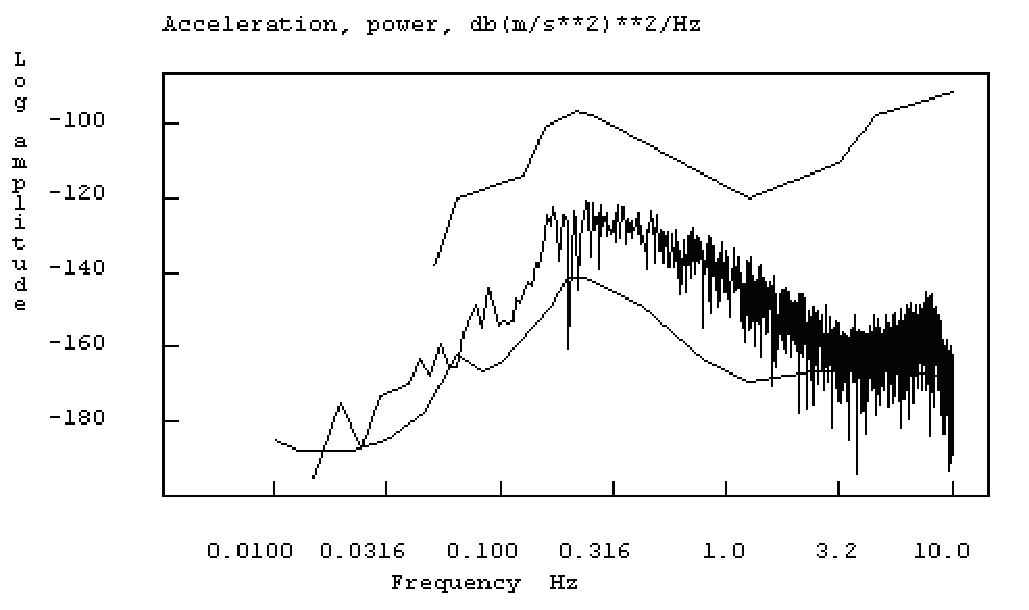
\includegraphics[width=0.9\linewidth]{fig/fig23}}
\caption{Example of a noise spectrum.}
\label{fig:noise-spec}
\end{figure}


\textbf{Problems:}
\index{Problem, MULPLT spectra}There is currently no check if a displacement seismogram has been calculated when calculating the spectral parameters. If spectral analysis is done outside EEV (output in \index{MULPLT.OUT}MULPLT.OUT) or with EEV when there is no origin time and/or epicentral distance, the output results are wrong for moment etc. Before calculating moment etc, the S-file MUST HAVE BEEN UPDATED SINCE BOTH THE DISTANCE AND ORIGIN TIMES ARE USED. If the spectra get very high amplitude levels when correcting for instrument, this might be caused by correcting for Q. With a Q of 100 and a distance of 10 000 km, this gives a very large correction. The Q-correction can be disabled in the \texttt{MULPLT.DEF} file. If picks are made, but no readings appear in the S-file or readings appear with wrong component, the waveform file component might not have been defined in subroutine componen.for. If poles and zeros are used to remove the response,\index{Problem, rotation} rotation cannot be used at the same time. 

\begin{figure}
\htmlimage{scale=2.0}
\centerline{\includegraphics[width=0.9\linewidth]{fig2/fig4a}}
\caption{Spectral analysis\newline
On top the original trace is seen and on the bottom the 
displacement spectrum (log -log, unit nm-sec and Hz). The level 
and slope has been indicated interactively. Note the noise spectrum 
at the bottom of the figure.}
\label{fig:mulplt-spec}
\end{figure}

\begin{figure}
\htmlimage{scale=2.0}
\centerline{\includegraphics[width=0.9\linewidth]{fig2/fig4b}}
\caption{Three component analysis\newline
On top the Z-channel is shown together with the window used for the 
3 channels Z, N and E shown below. The signals below has been filtered 
between 1 and 5 Hz and the resulting azimuth of arrival is 160 degrees 
and a correlation coefficient of 0.2. The apparent velocity is 9.8 km/sec.}
\label{fig:mulplt-3comp}
\end{figure}

\begin{figure}
\htmlimage{scale=2.0}
\centerline{\includegraphics[width=0.9\linewidth]{fig2/fig4c}}
\caption{Plotting response curves\newline
The figure shows the amplitude and phase response for station SUE, 
component S Z. The response is the one which will be used in analysis 
irrespective of whether it is taken from the file header or the CAL directory.}
\label{fig:mulplt-resp}
\end{figure}

\subsection{Particle motion plots}

Particle motion plots can be made in multi trace mode when three components from one station are selected. The particle motion is plotted below the rescaled trace plot. The particle motion plots are made for the time window shown in the trace plot. The trace plot has all the normal functionality, so it is still possible to zoom and filter. The particle motion plots can be useful when determining phase types. No readings can be made from the trace plots. 

\begin{figure}
\htmlimage{scale=2.0}
\centerline{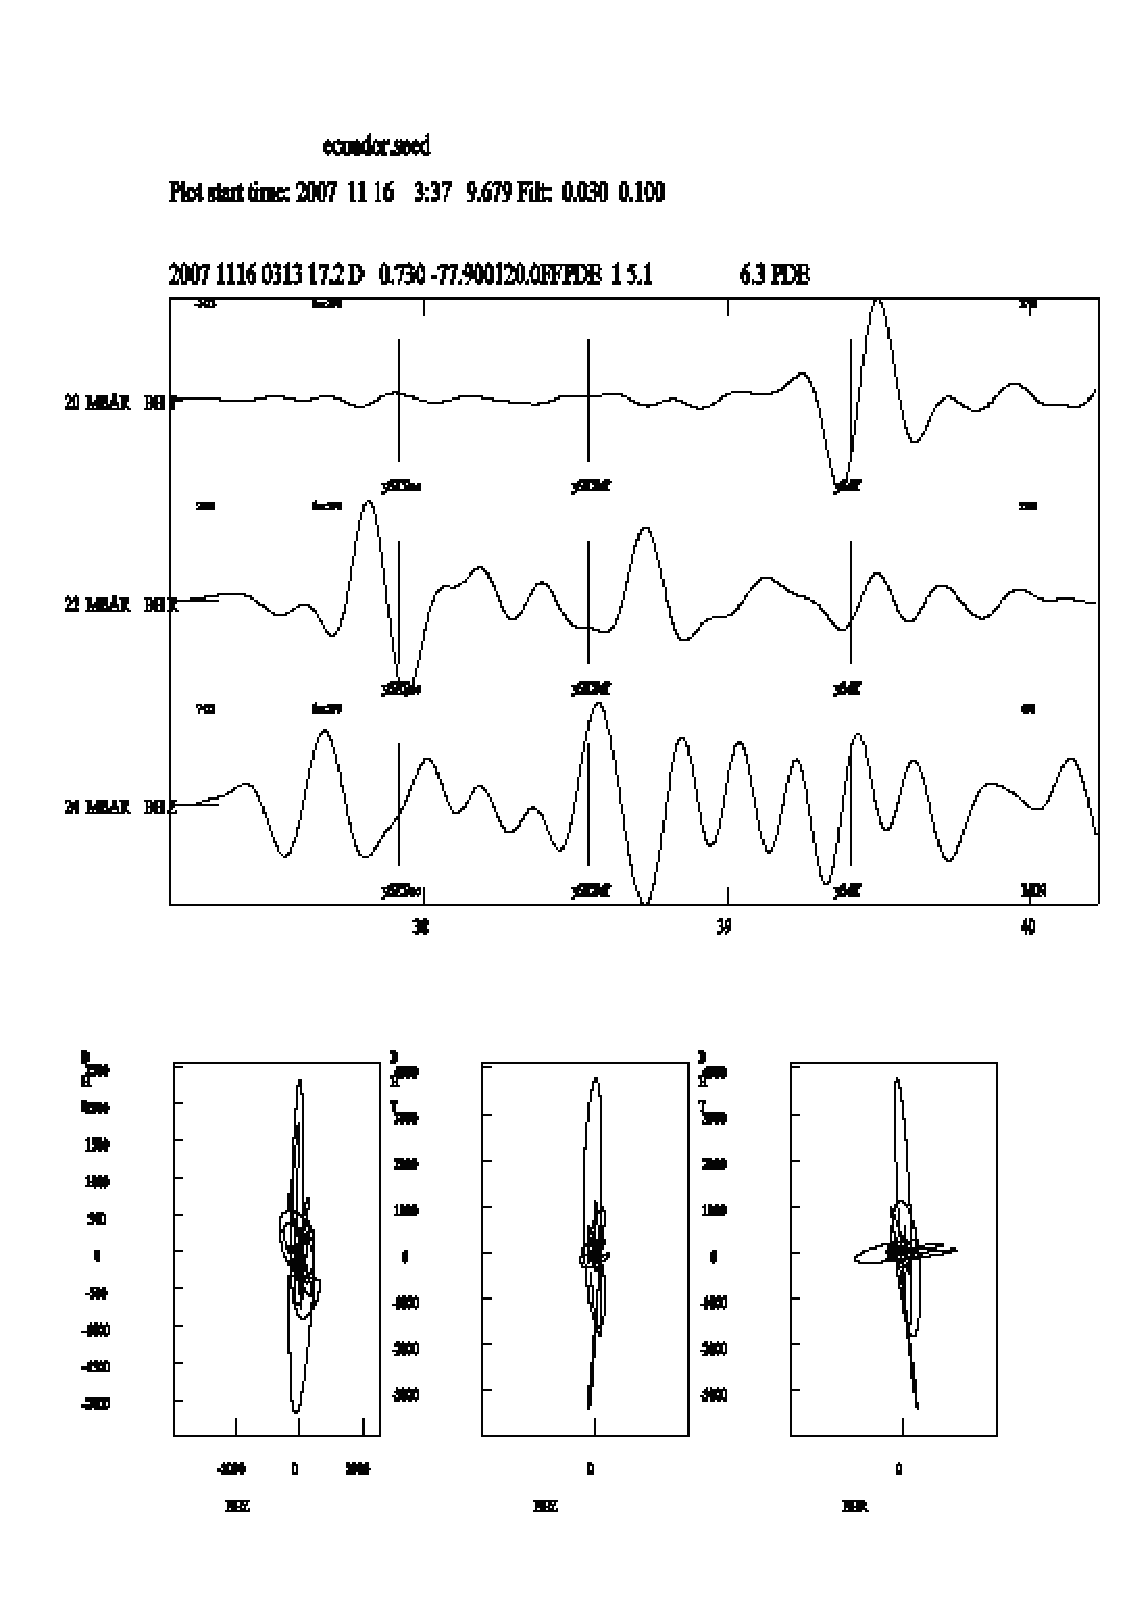
\includegraphics[width=0.9\linewidth]{fig/fig27}}
\caption{Example of particle motion plot.}
%\label{fig:}
\end{figure}

\subsection{The \texttt{MULPLT.DEF} and \texttt{SEISAN.DEF} files}
\index{MULPLT.DEF}\index{SEISAN.DEF}

In the \texttt{MULPLT.DEF} and the \texttt{SEISAN.DEF} files, it is possible to set the various parameters for MULPLT. Nearly all parameters are set in the \texttt{MULPLT.DEF} except geometrical distance parameters, which are set in \texttt{SEISAN.DEF} since these parameters also are used by HYP. MULPLT will operate without DEF-files using \index{Hardwired constants}hardwired defaults. The \texttt{MULPLT.DEF} can be located in the working directory and or in DAT. The if a DEF-file is present in the working directory, it overrides the file in DAT. In \texttt{MULPLT.DEF}, several groups of parameters can be set: The keyboard, default channels to use and analysis parameters (e.g. for spectral analysis). The parameters are identified by keywords, see example file below for explanation.
%\textcolor{red}{jh-change: 
Note that all numbers given in file are real and must be given a '.'

Example file: 

This file is for defaults for MULPLT and called \texttt{MULPLT.DEF}. 
The name must be in upper case on SUN. The following shows the parameters, 
which can be set. The file can contain any number of lines in any order, 
only the lines with recognized keywords and a non blank field under 
Par 1 will be read. 
%\textcolor{red}{pv-change: 
Numbers under Par1 and Par2 must be given as reals.
The comments have no importance. 

%\verbatiminput{include/MULPLT.DEF}
\verbatiminput{../seismo/DAT/DAT/MULPLT.DEF}

All parameters are within column 41 and 60 and each occupying up to 10 characters. 

NOTE: If any of the phase or weight keys are redefined, all previous \index{Defaults}defaults disappear. 

\index{Default channel}\textbf{DEFAULT CHANNEL}: All channels are default if not given. For routine display, it is useful to only select some channels. 

\index{Phase name key}\textbf{PHASE NAME KEY}: The keys associated with given phases. Remember that I, E or a blank MUST be part of the name so it is not possible to chose a name like "P", it must then be " P" (note the blank in front of P). About 10 phase combinations are currently default as seen on the pick display. If a new phase key is selected, you must define all the keys you want to use for phases including all the predefined phases. The combined onset/phase key can be up to 9 characters. 

\index{Phase weight key}\textbf{PHASE WEIGHT KEY}: The defaults are upper 
case 1,2,... to 0 for weights 1,2,... to 0 . Again, choosing just one other 
key, and all must be redefined. The symbol must be in column 41 and the 
weight in column 51. The weight is an integer 0, 1,2,3, 4 or 9. 

\index{Phase mouse key}\textbf{PHASE MOUSE KEY}: The default is blank. Normally no redefinition is needed since the mouse character is defined in SEISAN. The key can be defined as a character or the ASCII code written as a real number. 

\index{Spectral parameters}\textbf{SPECTRAL P-VELOCITY}: P-velocity in km/sec, default 6 km/sec 

\textbf{SPECTRAL S-VELOCITY}: S-velocity in km/sec, default  3.5 km/sec Both above parameters must be set separately, the Vp/Vs in \texttt{STATION0.HYP} is not used to calculate one from the other. The values go into the S-file the first time spectra are calculated. if values are changed later in the \texttt{MULPLT.DEF} file, no change will be made in the S-file, old values remain. 

\textbf{SPECTRAL Q0}:  $Q$ is defined as $q0 * f**qalpha$, default 0 meaning no Q-correction 

\textbf{SPECTRAL QALPHA }: See above, default 1.0, NOTE: Q is only used when doing spectral analysis and has no effect on the displacement seismograms. 

\textbf{SPECTRAL DENSITY}: Density for spectral analysis (g/cm**3), default 3.5 g/cm**3 

\textbf{SPECTRAL KAPPA}: Near surface attenuation, default 0.0 meaning no attenuation. For teleseismic events, this is t*. 

\textbf{SPECTRAL GEO\_DEPTHS}: Depth range where geometrical spreading changes from surface wave to body wave spreading, S-waves only. Default 50 and 100 km. This is only used if distance is larger than HERKIJ\_DISTANCE. THIS PARAMETER IS NOT SET IN \texttt{MULPLT.DEF}, BUT IN \texttt{SEISAN.DEF}, MENTIONED HERE SINCE IT IS IMPORTANT FOR SPECTRA. 

\textbf{HERKIJ\_DISTANCE}: \index{Herkij\_distance}Epicentral distance at which geometrical spreading changes from body wave spreading to surface wave spreading, S-waves only. Default 100 km.  THIS PARAMETER IS NOT SET IN \texttt{MULPLT.DEF}, BUT IN \texttt{SEISAN.DEF}, MENTIONED HERE SINCE IMPORTANT FOR SPECTRA 

\textbf{3COMPVELOCITY}: Velocity used (km/sec) in 3 component azimuth analysis. Default is 5 km/sec. 

\textbf{CHANNEL SORTING}: If set to 1.0, channels and filenames are sorted alphabetically, if 0.0, no sorting. Default = blank is sorting. 

\textbf{NCHAN PER SCREEN}: The number of channels to be displayed per screen. 
Default = blank is 99 channels. 
%\textcolor{red}{pv-change: 
It may conflict with \textbf{DEFAULT CHANNEL}.

\textbf{NSORT\_DISTANCE}: If blank or zero, channels are plotted in 
the order as they appear in the waveform file 
%\textcolor{red}{jh-change:
or in alphabetical order if flag CHANNEL SORTING is set. 
If set to 1.0, the channels are plotted in 
%\textcolor{red}{jh-change: 
distance order if a distance is given in S-file. 
If not plotted from EEV, 1.0 will indicate sorting in 
waveform file header time order. Default 0.

\textbf{X\_SCREEN\_SIZE}: Size of initial X-window in \% of total screen. Default 90 \%. 

\index{Resolution}\textbf{RESOLUTIONX and RESOLUTIONHC is the number of points plotted on the screen or laser printer respectively. If e.g. 1000 points are plotted, this means that the remaining points are skipped although some primitive smoothing is done. Choosing too few points can lead to funny looking seismograms with aliasing effects and using all points will slow down the plotting. Resolutionx is for the screen and resolutionhc for the hardcopy. NOTE}: If using MULPLT mode where both screen and hardcopy is used, it is the hardcopy resolution, which is used for both. Default 1000 and 3000 respectively. 

\textbf{SPECTRAL F-BAND}: Spectral range (Hz) used for spectral plots. Default values are 0.05 to 20.0 Hz. 

\index{AUTO\_PROCESS}\textbf{AUTO\_PROCESS}: Immediately following registration, MULPLT can run any program specified here. Since the event name has been put into memory, the program can operate on the newly \index{Preprocessing of data}registered S-file. Parameter one has the options: 0: Do not auto process, 2: Ask the user if autoprocess, 3: Autoprocess without asking the user. Parameter 2 gives the name of the process to run. The name is limited to 10 characters. Default, no auto processing. 

\index{AUTO\_LOCATE}\textbf{AUTO\_LOCATE}: Immediately following registration, MULPLT can locate the newly registered event and put the location into the database. Parameter one has the options: 0: Do not locate, 1: Ask the user if locate, 2: Locate without asking the user. Parameter 2: 0: Do not save in database, 1: Ask if saving in database, 2: Automatically save in database. Default, no auto locate. 

\textbf{SPECTRAL OUTPUT}: If parameter set to 1, two output files are created for each signal spectrum. \texttt{com\_spec.out} is the complex spectrum and \texttt{amp\_spec.out} is the real spectrum. Default 0.0. In addition, the single trace zoom window is saved in signal.out. 

\textbf{FILTER}: Change definition of filters 1 to 7. The settings affect both the shortcut keys and the menu boxes. 

%\textbf{FILTER TYPE}: Choice between two different filter routines 
%that basically do the same. Use 0.0 for routine 'bndpas' (default) 
%and 1.0 for 'recfil'. Bndpas is a recursive Butterworth bandpass 
%filter routine. Recfil is an IIR filter routine (various filter 
%types supported, but in SEISAN only Butterworth is used), which 
%works as low-, high- or band-pass, however, gives problems for 
%bandpass at low frequencies. Low- and high-pass when using recfil 
%are given by setting either the upper or lower frequency limit to 
%0.0, respectively. 
%\textcolor{red}{jh-change:  
%have remove wa high cut, filters for ms and mb}

\textbf{ML LOW CUT AND POLES and ML HIGH CUT AND POLES}: 
Filter band for Wood Anderson 
%\textcolor{red}{jh-change: 
additional 
filter. Recommanded values are 1.25 Hz to 20 Hz and 4 poles. Note poles for high cut and low cut must be equal, if not lowest value is used. 

\textbf{BANDPASS FILTER}\index{Bandpass filter, default in mulplt}\index{Default filter}: When using all 
defaults from EEV (option PO), a bandpass filter can be set. Default is no filter. The parameters are 
lowcut and highcut for parameter one and two respectively. 4 poles only. 

\textbf{FIX FILTER}\index{Fix filter in mulplt}: When using alldefaults from EEV (option PO), a bandpass filter can be set, see parameter BANDPASS FILTER. The filter can be fixed with paramter FIX FILTER: 1.0 =fix filter, 0=no fix. Fixing means that in all operation the filter will remain.

\textbf{CODA AUTO}: Enable automatic coda determination (YES or NO). Default is NO. If enabled, auto coda is read with c instead of C. 

\textbf{AUTOCODA FILTER }: Filter band for automatic coda: Default 5 to 10 Hz. \index{Coda length}\index{Automatic coda length}AUTOCODA STA : Auto coda short term average: Default 5.0 secs. 

\textbf{AUTOCODA RATIO }: Autocoda ratio. Default 1.5.

\textbf{MULPLT AREA }: Options for plotting stations in a given distance from a midpoint. 0: do not select option (default) 1: midpoint from s-filei epicenter, radius from MULPLT.DEF,  2: midpoint from MULPLT.DEF, radius interactive  3: midpoint and radius from MULPLT.DEF, 4: midpoint from MULPLT.DEF, radius interactive, 5: midpoint and radius interactive 

\textbf{MULPLT LAT LON }: Midpoint 

\textbf{MULPLT RADIUS }: Radius in degrees 

\subsection{Distance trace plot with GMT, TRACE\_PLOT (Unix only)}
\index{TRACE\_PLOT}\index{Trace plotting}
TRACE\_PLOT is a simple program to create a distance trace plot using GMT programs (Generic Mapping Tools, \url{http://gmt.soest.hawaii.edu/}). The axes of the plot are time and distance, and the traces are centered on the respective epicentral distance. The input to the program is a single event in Nordic format (S-file). From the S-file, the program reads the origin time, epicenter location and the names of the associated waveform files. TRACE\_PLOT reads the waveform data and writes the x-y coordinates of the lines in the plot to a file that is then used as input to the GMT program psxy. The TRACE\_PLOT program removes the DC from the data and as an option can apply a band-pass filter. The output of the program is a Postscript file (\texttt{trace\_plot.ps}) and a batch file that can be modified and used to rerun the GMT programs (\texttt{trace\_plot.bat}). The parameters are set in the \texttt{trace\_plot.par} file, which can be located either in the DAT or in the working directory. An example is seen in Figure 
\ref{fig:mulplt-3comp}
. 

The parameters in \texttt{trace\_plot.par} are: 

FILTER: The pass-band filter limits can be specified through the FILTER parameter.\newline
DISTANCE: The distance range (y-axis) for the plot.\newline
TIME: The time range in seconds (x-axis).\newline
AMPLITUDE\_SCALE: The amplitudes are scaled for every trace individually, by  [amplitude/(max 
amplitude) * AMPLITUDE\_SCALE]. \newline
STATION\_SFILE\_ONLY: This variable can be set to 1.0 to only plot 
traces that are listed in the S-file, the default is 0., which plots 
all traces without checking if they are present in the S-file. \newline
TIME\_ORIGIN: In the current version, the origin of the time axis 
corresponds to the origin time of the event. \newline
COMPONENT: This can be used to select components for plotting, in case no component is defined, TRACE\_PLOT will show all vertical component traces. 

Example of \texttt{trace\_plot.par}: 

\verbatiminput{include/trace_plot.par}



%\textcolor{red}{pv-change: 
\section{Plotting epicenters} 
In SEISAN there are three different programs for plotting epicenters, 
EPIMAP, W\_EMAP and GMAP. 
EPIMAP is the basic program for plotting epicenters in SEISAN and 
is the program that is called from EEV, when you type \texttt{map}.
W\_EMAP is a windows based program.  
GMAP is linked to the Google Earth and Google Map Internet mapping tool.
%}


\subsection{EPIMAP} 

The command for plotting epicenters is \index{EPIMAP}EPIMAP <file>, where the optional file is a file with EPIMAP commands. If file is not given, the user will be prompted for the input. The program can plot land contours, epicenters, macroseismic intensities, stations and level contours as well as depth profiles. It is possible to zoom in on selected areas (option by \textbf{Mario Villagr\'an}). The program has been much revised by \textbf{Jim Bolton}. 

Input files: Land contours and other contours 

The program will look for all files ending with .MAP located in the DAT directory. The user can then choose any one or a combination of files\index{Plot contours}. The users own contour files (e.g. faults) can be added to the DAT directory. A very detailed world map is available on the SEISAN CD and on the SEISAN web site. Areas can be selected out of these files with program SELMAP. 

Stations 

Epimap will look in \texttt{STATION0.HYP} for station coordinates. It will search first in the working directory, then in DAT. 

Epicenters 

The user will be prompted for epicenter input files. The format can 
be Nordic or Nordic compact. Magnitudes are plotted proportional with 
symbol size unless the ellipticity option is selected in which case 
the error ellipses are plotted (if smaller than 100 km).
%\textcolor{red}{jh-change:
Fault plane solutions can optionally be plotted instead of error 
ellipses. The first fault plan esolution found in file will be used. Name of 
intensity files (SEISAN standard format, see Appendix \ref{app:nordic}) are also 
entered here. The file name must have the 3 letters `mac' after the `.' 
See also section \ref{sect:macro}. 

Input files for EPIMAP can be made e.g. with the COLLECT command which collects S-files into one file or with the SELECT command selecting data from the database using several criteria.  HYP also generates a CAT-file (\texttt{hyp.out}) which may be used as input to EPIMAP. 

Macoseismic information 

EPIMAP can plot SEISAN macroseismic observations, see section \ref{sect:macro}.

Magnitudes 

The program will read all 3 magnitudes (magnitude1, magnitude2 and magnitude3) in the header line. It will use the first non-zero magnitude in the order magnitude1, \index{Magnitude in epimap}magnitude3 and magnitude2. Epimap will search the first header line only. If it is desired to use a particular magnitude from any header line for plotting, use MAG program first to select particular magnitude type which is then placed in first header line magnitude position one. Program NORHEAD can move magnitudes from following header lines to the first line. Program REPORT can move magnitudes around on the header line. 

A typical run is as follows, comment after !: 

\verbatiminput{include/epimap.run}

\textbf{Interactive options}: 

When the plot is shown, there appears in the lower left-hand corner a menu of several options: 

Q: Quit \newline
P: Profile \newline
A: Area \newline
Z: Zoom 

Press one of the letters to continue. 

P: Profile 

One or seve\index{Depth profile}\index{Profile, hypocenters}ral depth section windows can now be selected with the cursor. First move the cursor to where the section shall start (from where distances are calculated), press any character to select point, move cursor to end of profile, press any character to select. A line between the two points is now plotted. Move the cursor to a point on the side of the line and press any character. A rectangle defined by the three points is now drawn, which defines the area used for the section. If more than one section is wanted (up to 9), press the number of sections instead. The selected number of profile boxes will now be plotted, all the same size.  Pressing any character will draw the depth sections \index{Autoscale depth profile}auto scaled, while PRESSING THE CHARACTER F, THE X AND Y SCALES ARE EQUAL and determined by the horizontal extension. When the first section appears, you can either press q to quit or any other character to plot next profile or, if the last profile, replot epicenter map and select new sections. IF YOU WANT ALL SECTIONS TO REMAIN IN PLOT FILE, QUIT AFTER PLOTTING THE LAST PROFILE. The plot file always stores what has been plotted so far, and is overwritten when a replot is made. It is also possible to plot a previously defined profile by entering O. The parameters are then taken from file profile.out. This file stores the last parameters selected by EPIMAP, but can also be edited by the user. 

A: Area 

Select, by clicking with the cursor, at least 3 points defining a polygon within which epicenters are selected. A new plot is made enclosing only the polygon and showing the epicenters within the polygon. The corresponding epicenters (S-files) are in file epimap.are. \index{Selection in polygon}\index{Polygon, select in}Known bug: \index{Problem, MULPLT area}Sometimes epicenters are still left outside, SELECT can be used instead. 

Z: Zoom 

Similar to Area, however a rectangle is selected by defining just the 2 diagonal corners. 

%\textcolor{red}{jh-change:
MAP files
The map files consist of blocks of coordinate pairs. Each block starts with the number of pairs in the block. The format of the header line is i4 and the following lines 10f8.3. Thus each block can at most have 9999 pairs.

Plotting place names \index{Place names}\index{Plotting place names}If option P is used when the program asks for place names or station codes, the user will be prompted for one or several files with place names. The place name file format is: 

name latitude\_degrees longitude degrees 

eg: 

\begin{verbatim}
Edinburgh    55.94422  3.20096   or
Edinburgh   55.94422   3.20096   etc.
\end{verbatim}

The only requirement is that at least 2 blanks separate the place 
name and the geographical co-ordinates. Note that the place name 
can contain one or more blanks, however each blank must occur singly. 
%\textcolor{red}{jh-change:  
An example of a place name file is place\_names.macro located in DAT.
Epimap contour file\index{Contour file} 
EPIMAP has a simple contouring routine accepting a regular spaced grid. Below is an example (output from EQRSEI). The top part of the file is just comments, the data starts at "Fields to use". The data must come in longitude, latitude pairs (+ value of contour) in order as shown below. The contour value is plotted exactly as shown below. E. g. the value 117 is plotted as \_\_117\_\_\_\_\_ where "\_" is blank. By specifying \_\_\_\_117.0\_, the value would be plotted as 117.0 and moved one space to the left on the plot. Currently only programs EQR\index{EQRSEI}SEI (version 7.0) and C\index{CRISEI}RISEI from SEISAN version 6.0 make contour files. In the DAT directory, there is an example of an EQRSEI.OUT file 

NB: In the input file shown below, the FIRST COLUMN MUST BE blank. 

\verbatiminput{include/epimap.input}

\textbf{EPIMAP output files:}

\texttt{epimap.out}: Gives a numbered list of all events within main window. This can be used in connection with the number option. 

\texttt{epimap.cor} and \texttt{epimap.are}: If option A (selecting area) has been used, the coordinates of the corners will be given in \texttt{epimap.cor} and the complete events (S-files) within the selected area, in \texttt{epimap.are}. \index{Epimap.cor} 

\texttt{epimap.num}: A compact file of \texttt{epimap.out} with the numbers plotted.\index{Select epicenters in an area}\index{Epicenter area selection}\index{Epimap.num} 

\texttt{epimap.eps}: Postscript plot file of epicenters and possible profiles. If only one profile has been selected, all is on one page. If several profiles are selected, there will be two profiles per page up to a maximum of 6 pages (one with map and 5 with profiles). 

\texttt{epimap.inp}: This file is storing all input parameters of the run and can be used to run epimap again without entering any \index{Epimap.inp}parameters. The file can be edited if a run has to be repeated with e.g. a new epicenter file. The file can have any name so several predefined plot definitions can be stored and thereby automate\index{Automate EPIMAP} map production. 

\texttt{profile.out}: The \index{Profile.num}file stores the parameters used with the profiles. The file is overwritten for each new profile parameter selection. An example is: 

\begin{verbatim}
  60.93583   7.21519  63.29655   1.36709  63.39875   5.01266
      27.8
         3
\end{verbatim}

The first line gives latitude and longitude of the 3 points used for selecting profile (see explanation for interactive section), next line the azimuth calculated for the profile and the last line gives the number of profiles. The file can be used to repeat the same profile as in an earlier run or to predefine a more exact profile than can be selected with the cursor. 

\texttt{profile.num}: \index{Profile.num}Output of distance and depth of the profile in km. Distance is only correct in unzoomed plots. 

Problems: Known bug: When selecting events with polygon, sometimes some events remain outside\index{Problem, EPIMAP} 

Figure 
\ref{fig:epimap}
and Figure 
\ref{fig:epimap-area}
shows examples of plots made with EPIMAP. 


\begin{figure}
\htmlimage{scale=2.0}
\centerline{\includegraphics[width=0.9\linewidth]{fig2/fig5a}}
\centerline{\includegraphics[width=0.9\linewidth]{fig2/fig5aa}}
\caption{An example of using EPIMAP. The top shows epicenters plotted and the bottom the first of a series of profiles. The frames on the top plot show the location of the profiles. 
}
\label{fig:epimap}
\end{figure}

\begin{figure}
\htmlimage{scale=2.0}
\centerline{\includegraphics[width=0.9\linewidth]{fig2/fig5b}}
\caption{An example of using EPIMAP with area selection. The top plot shows where the area is selected, while the bottom plot shows the selected area. 
}
\label{fig:epimap-area}
\end{figure}




\subsection{W\_EMAP, Version Windows based map program} 

Program and documentation by \textbf{Fernando Carrilho}, fernando.carrilho@meteo.ptu\newline
Program must be installed in addition to SEISAN.

\index{Fault plane solution, plot}\index{Plotting epicenters} 
This program was developed to be used on seismic routine processing. Its main features are the capability of allowing visualization of epicentre locations, seismic stations, error ellipses, coastlines, macroseismic data, focal mechanisms (one or many) and simplified tectonics. From the previous public version (4.1), some bugs were corrected and new features added. In particular:  cartographic deformation is taken into account in error ellipses and station-epicentral path draws; some bugs on printing were corrected; compacted seisan files can be used within `additional events' representation; travel time curves can now be displayed; simplified relief can be displayed (if available as a MAP file); more than one file can be used for each category layer (coastlines, tectonic, relief and places names). 

The program can be integrated within the SEISAN environment, since it uses SEISAN parameter files, macrosseismic files, MAP files and station/model files. 

\begin{figure}
\htmlimage{scale=2.0}
\centerline{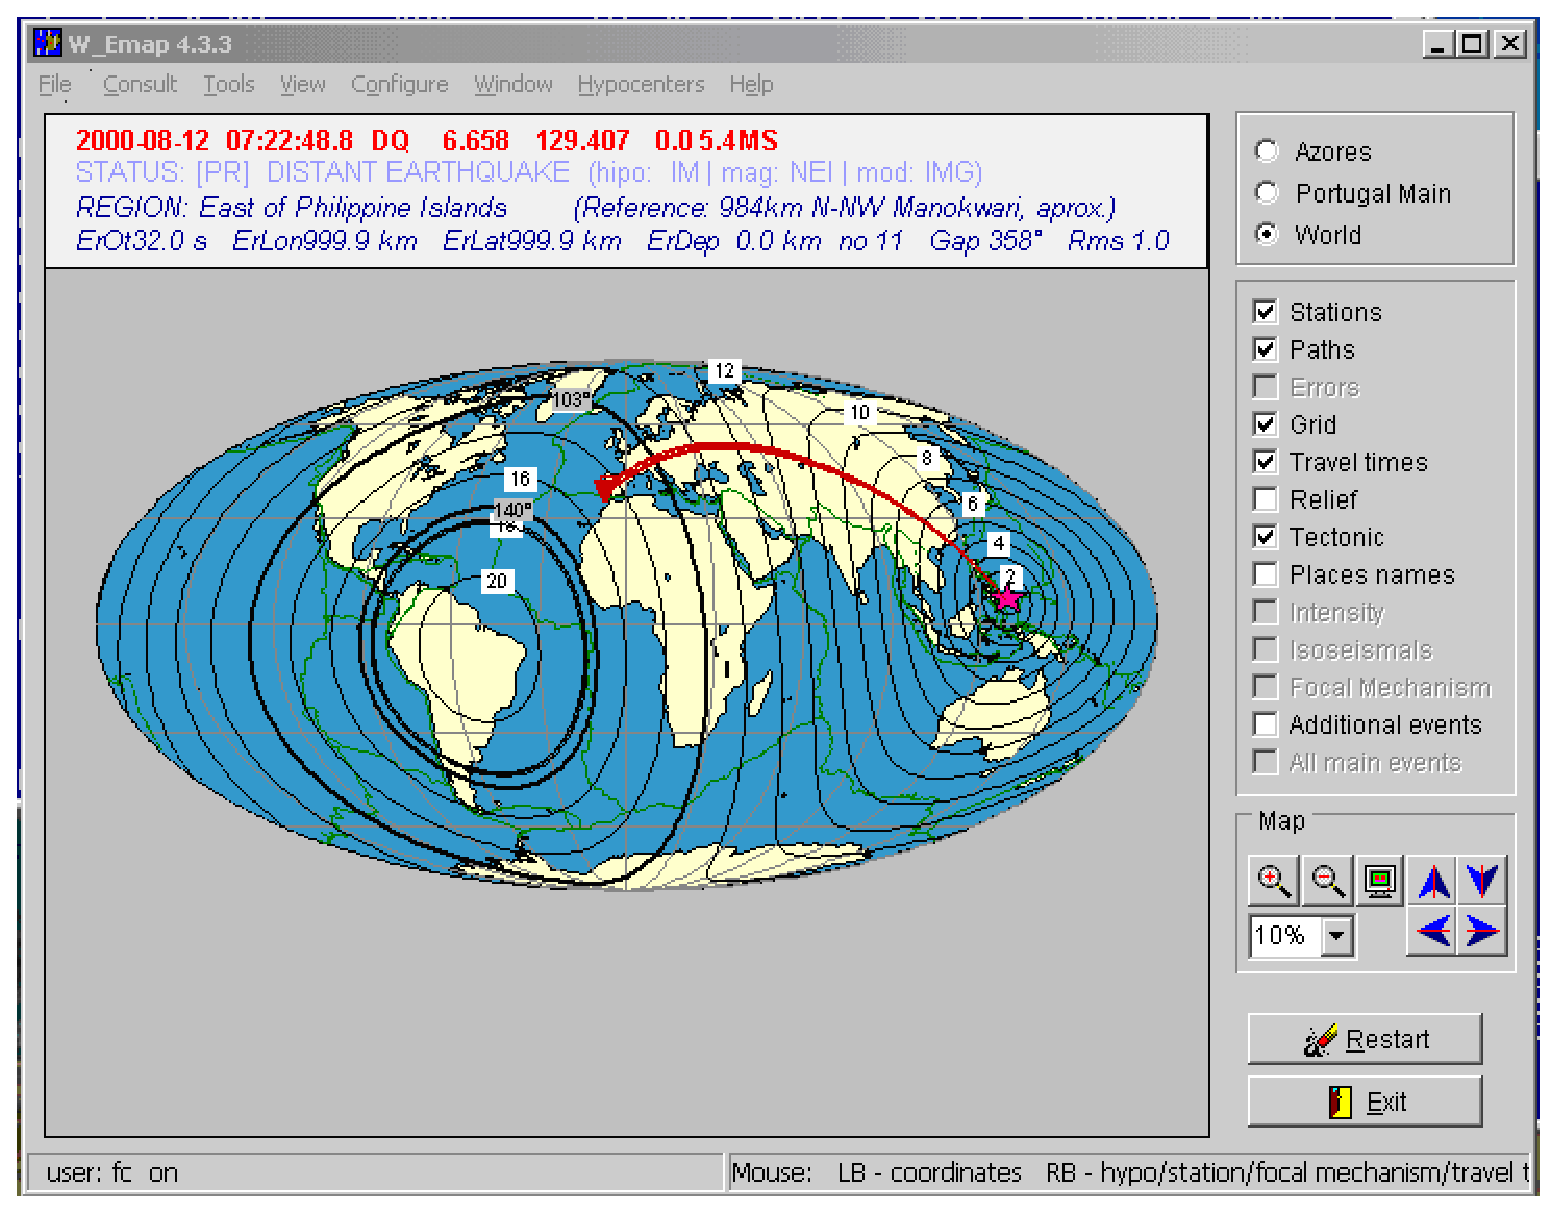
\includegraphics[width=0.9\linewidth]{fig/fig31}}
\caption{Example for plot using w\_emap (example not latest version).}
%\label{fig:}
\end{figure}


If the program is called from EEV or from the command line as W\_EMAP, then it displays information contained in \texttt{hyp.out} file, generated by the HYPOCENT \citep{lienert1994} location program, included in SEISAN, in the settable working directory. \newline
During the first run, user is driven to edit the configuration file w\_emap.def that is created in the users personal directory (SEISAN\_TOP/DAT/users/<username>), where most of the program parameters can be changed. \newline
The program can automatically detect changes in the \texttt{hyp.out} file so the user 
\underline{doesn't need to restart} the program each time the epicentre changes. \newline
The program can also display epicentres contained in any SEISAN parameter file, where the user may choose between one single epicentre and all epicentres at the same time. Double clicking the right mouse button will change the active epicentre to the one picked. 

Multi-user individual configurations (color schemes, additional event files, tectonic files, coastline files, relief files, cartographic projections, etc.) are supported. 
The program also has an option for Google Earth and Google map.. \index{Google Earth} Installation 
All the files are included in the distribution file w\_emap.exe. To install it, you just execute this install script and make sure W\_EMAP is installed under \_SEISMO\_TOP (Usually \\seismo). 
The manual will only be found in INF after installation. The current version of W\_EMAP is 4.8.2 but the manual has not been updated since version 4.6. 
An important new option is be able to directly plot a file with many hypocenters with the command w�emap filename. 
Known problem: Thre must be a type 7 line in S-file in order to be 
able to plot a focal mechanism. Some versions of w\_emap plot some 
of the fault plane solutions with inverted colors. \index{W\_EMAP} 




\subsection{GMAP, Plotting epicentres with Google maps or Google Earth} 
\label{subs:gmap}

%\textcolor{red}{jh-change:  peter: you name shoudl be removed everywhere in text sine you are now a coauthor. in gmap section describe browser used since firefox is harwired in eev, what if people use another ?}\newline
%\textcolor{green}{pv-change: firefox is nolonger hardwired in eev.}\newline
Google maps and Google Earth seem to quickly establish themselves as 
commonly used mapping tools. GMAP provides the conversion from Nordic 
format (s-files) to the input format required by these systems, 
which is the Keyhole Markup Language (KML). 
GMAP also convert SEISAN station and polygon files.
\index{Gmap}
\index{Google Earth}
\index{Google map} 
The input format of 
Google Earth is described on \url{http://earth.google.com/kml/}. 
GMAP required Google Earth installed on your system to plot 
the output file. Download Google Earth here 
\url{http://earth.google.com/download-earth.html} 
(note the terms and conditions on 
\url{http://pack.google.com/intl/en/eula\_print\_us.html}). 
To change the color codes se e.g. \url{http://html-color-codes.info/}.

% \href{http://earth.google.com/download-earth.html}{TEST}

GMAP can run in three modes: 
\begin{itemize}
\item The simple GMAP - runs in the browser with Google Map
\item The advanced GMAP - runs in the desktop version of Google Earth
\item The automatic GMAP - runs in the desktop version of Google Earth
\end{itemize}
The three modes are described below.

\subsubsection{The simple GMAP}
\index{GMAP simple} 
Type gmap in eev, a file \texttt{gmap.html} is created and copied to you 
GMAP\_DIR directory. When you open the \texttt{gmap.html} with your 
browser, you will be redirected to Google Maps and a green arrow will 
show the epicentre. The following parameters in \texttt{SEISAN.DEF} are used:
GMAP\_DIR /home/seismo/www\newline
GMAP\_TYPE MAP [MAP, SATELLITE, HYBRID or TERRAIN]\newline
GMAP\_TYPE determines which type of map Google MAPS will use, 
you can choose between: MAP, SATELLITE, HYBRID and TERRAIN. 

\subsubsection{The advanced GMAP}
\index{GMAP advanced} 
This mode of GMAP is a command line version, that convert SEISAN s-files to input 
files for Google Earth. It also convert SEISAN STATIONx.HYP files and polygone files.

\begin{itemize}
\item
Type \texttt{gmap} on the command line to start gmap.
\item
Type \texttt{gmap -help} to see the options. 
\item
Type \texttt{gmap -stat} to convert a SEISAN station files to kml. 
\item
Type \texttt{gmap -poly} to convert a SEISAN polygon files to kml. 
\end{itemize}

In \texttt{gmap} you can:
\begin{enumerate}
\item 
Set the colour of the icons. 
\item Show the error ellipse.
\item Show events as a animation over time. 
\item Set the scale of the icons (default: scale=0.2*mag**0.5). 
\item Set the type of icon used for earthquakes, explosions, probable explosions and for other events. 
\item Include or exclude the S-file. 
\item Rename the output file. 
\item Append text in KML format to the output file (See \texttt{SEISAN.DEF} parameters below). 
\end{enumerate}


Example: \newline
\begin{enumerate}
\item 
Use select to grap data from your Seisan database. 
\item Run the GMAP program:\newline
\begin{verbatim}
unix:/home/seismo/WOR: gmap 
 INPUT FILE NAME 
select.out 
Title: 
West Greenland [2000;2008]

Number of Earthquakes : 945 Explosions : 0 Probable Explosions : 2 Other events : 2 
Output file is
gmap.kml
\end{verbatim}

\item
In Google Earth open the output file gmap.kml. See Fig. \ref{fig:gmap}. 
\end{enumerate}

\begin{figure}
\htmlimage{scale=2.0}
\centerline{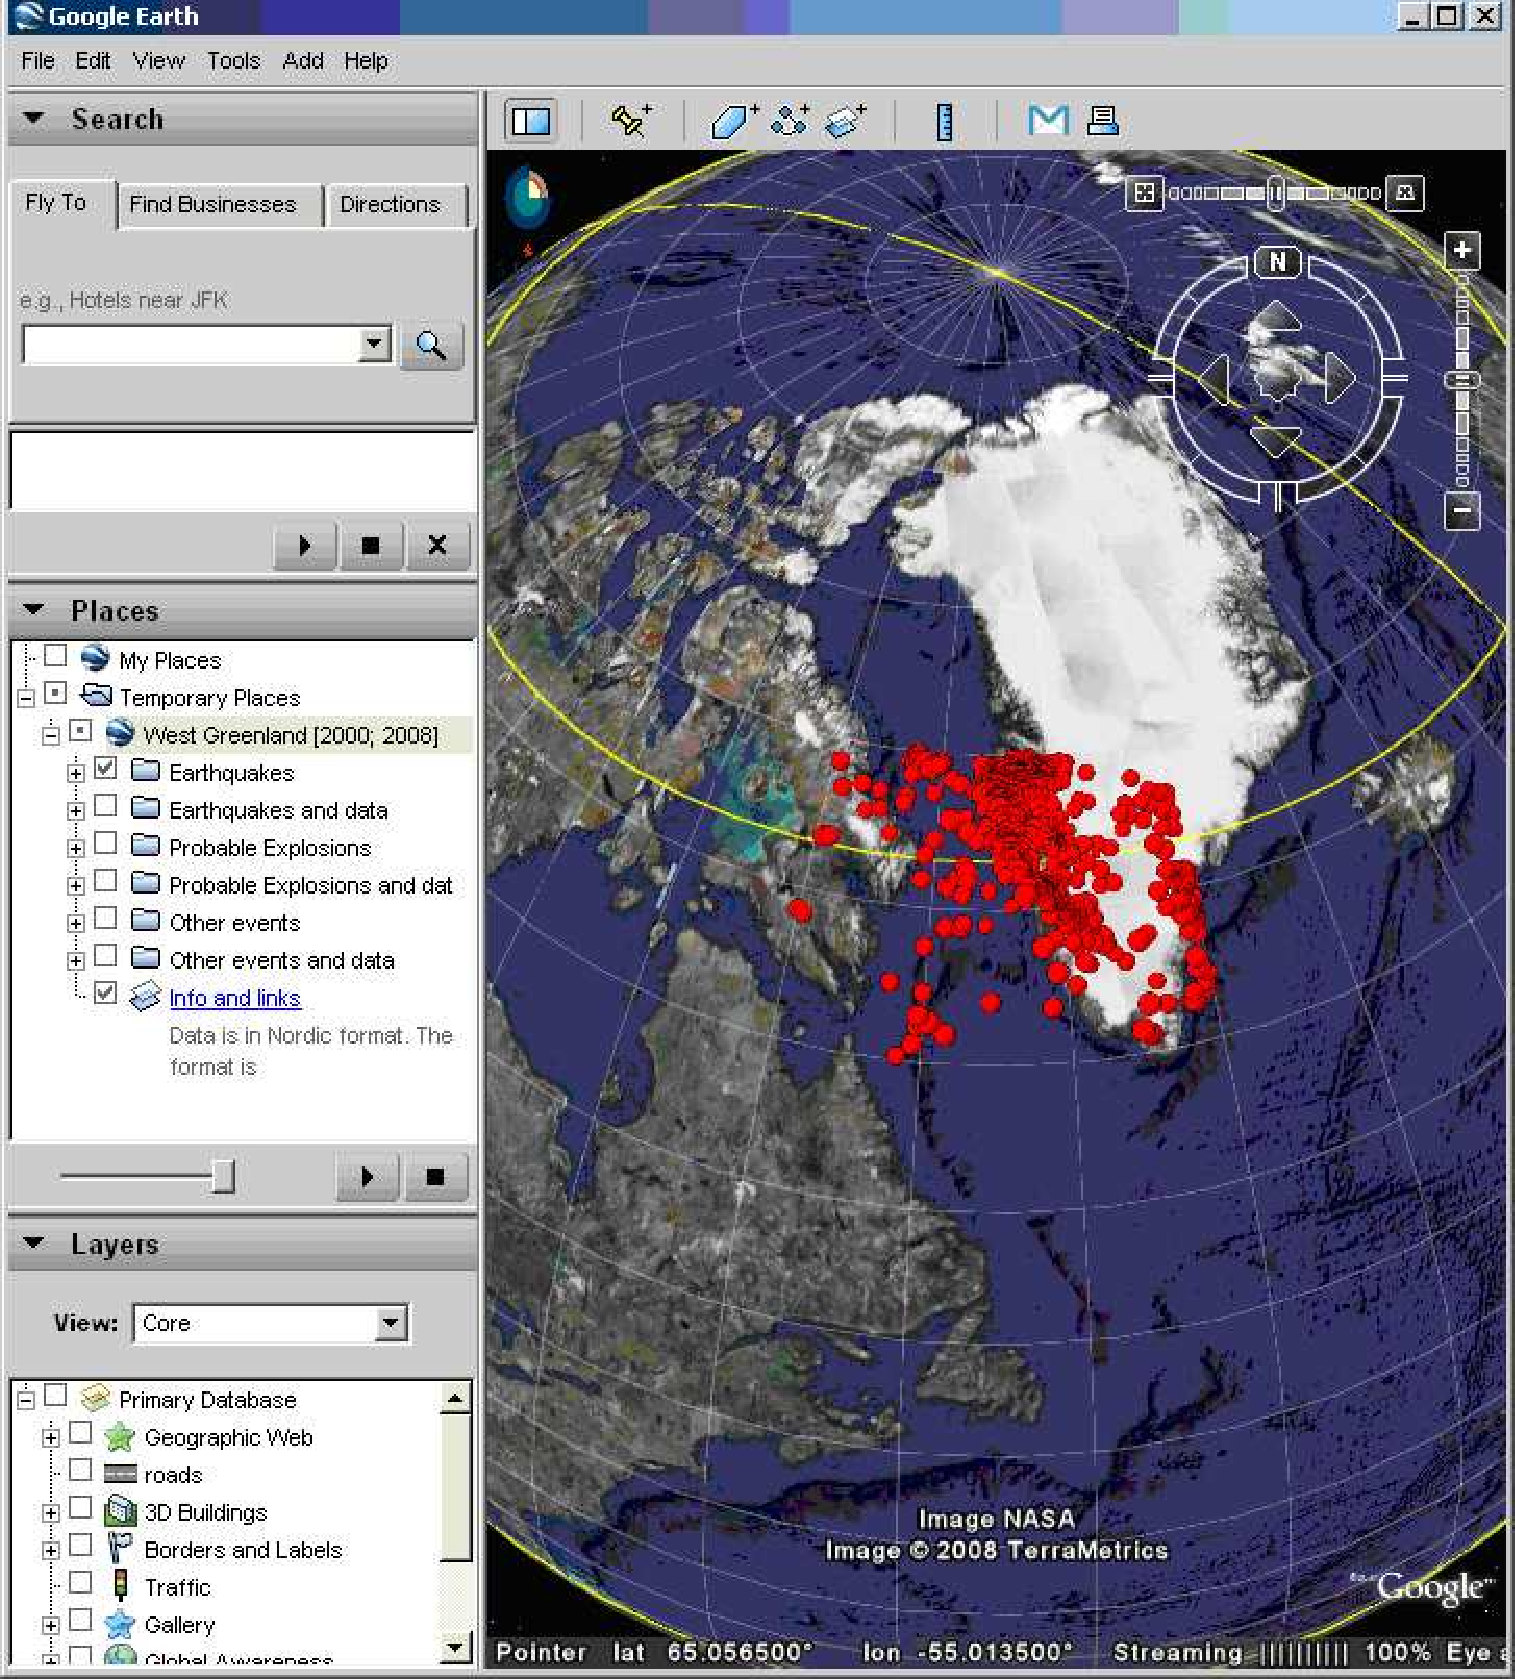
\includegraphics[width=0.9\linewidth]{fig/fig32}}
\caption{Example of mapping with gmap. Events in 
West Greenland. Note the folder and the subfolders in the \texttt{Places} window.}
\label{fig:gmap}
\end{figure}

To make an animation for events over time use the -timespan flag. As an example explosions in the south of Norway from 1983 to 2007 can be downloaded here: \url{http://seis.geus.net/ber-exp.kml} Press the play button at the time slider at the top of the Google Earth. Use the ruler to control how the animation is displayed (speed, days shown, etc.). 

\index{Raster file} 

\begin{figure}
\htmlimage{scale=2.0}
\centerline{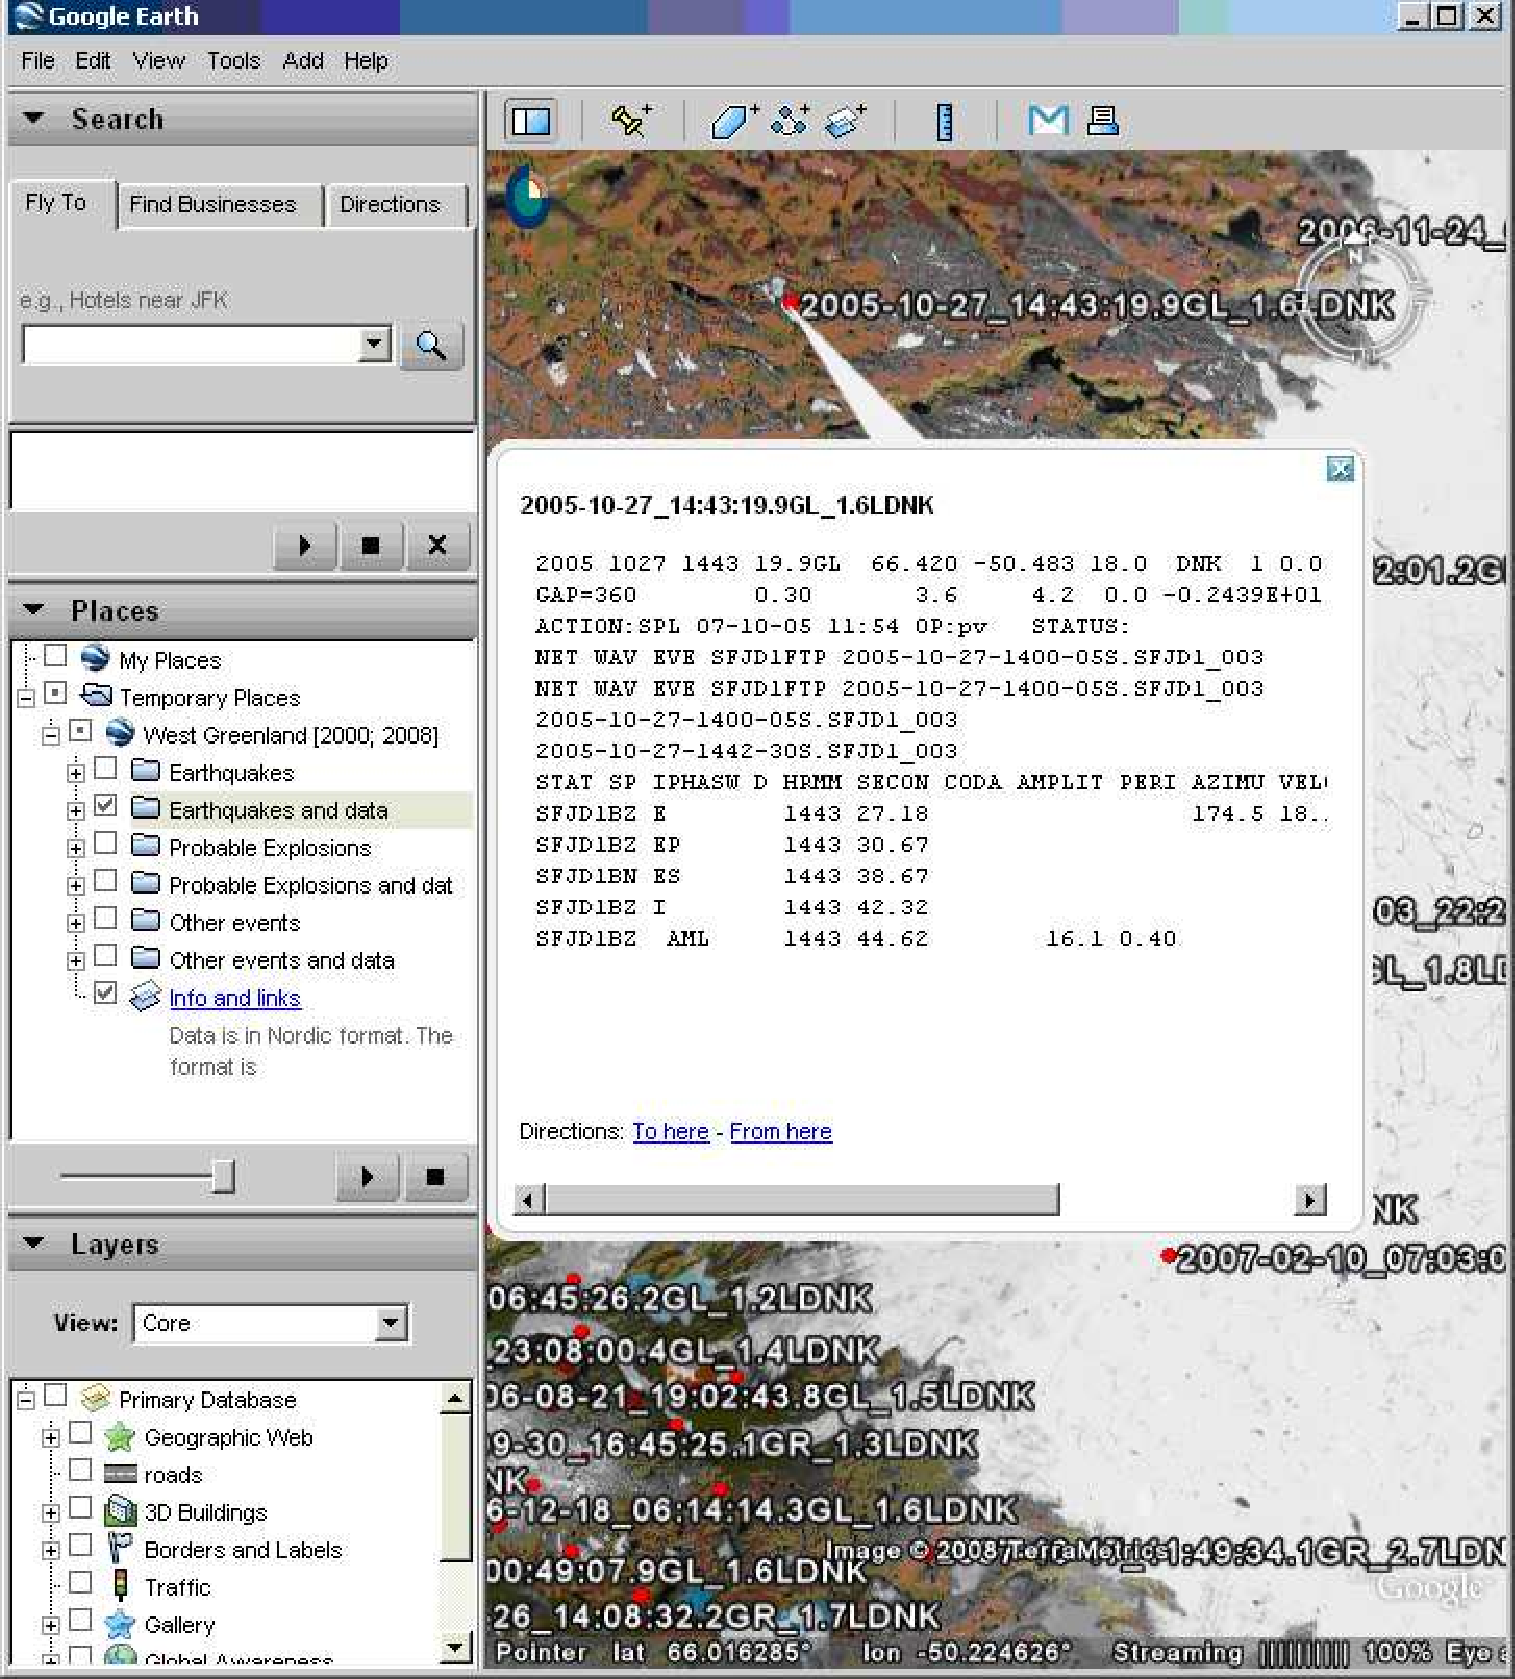
\includegraphics[width=0.9\linewidth]{fig/fig33}}
\caption{If the \texttt{Earthquakes and data} folder is selected in 
the \texttt{Places} window S-files can be shown.}
%\label{fig:}
\end{figure}

\begin{figure}
\htmlimage{scale=2.0}
\centerline{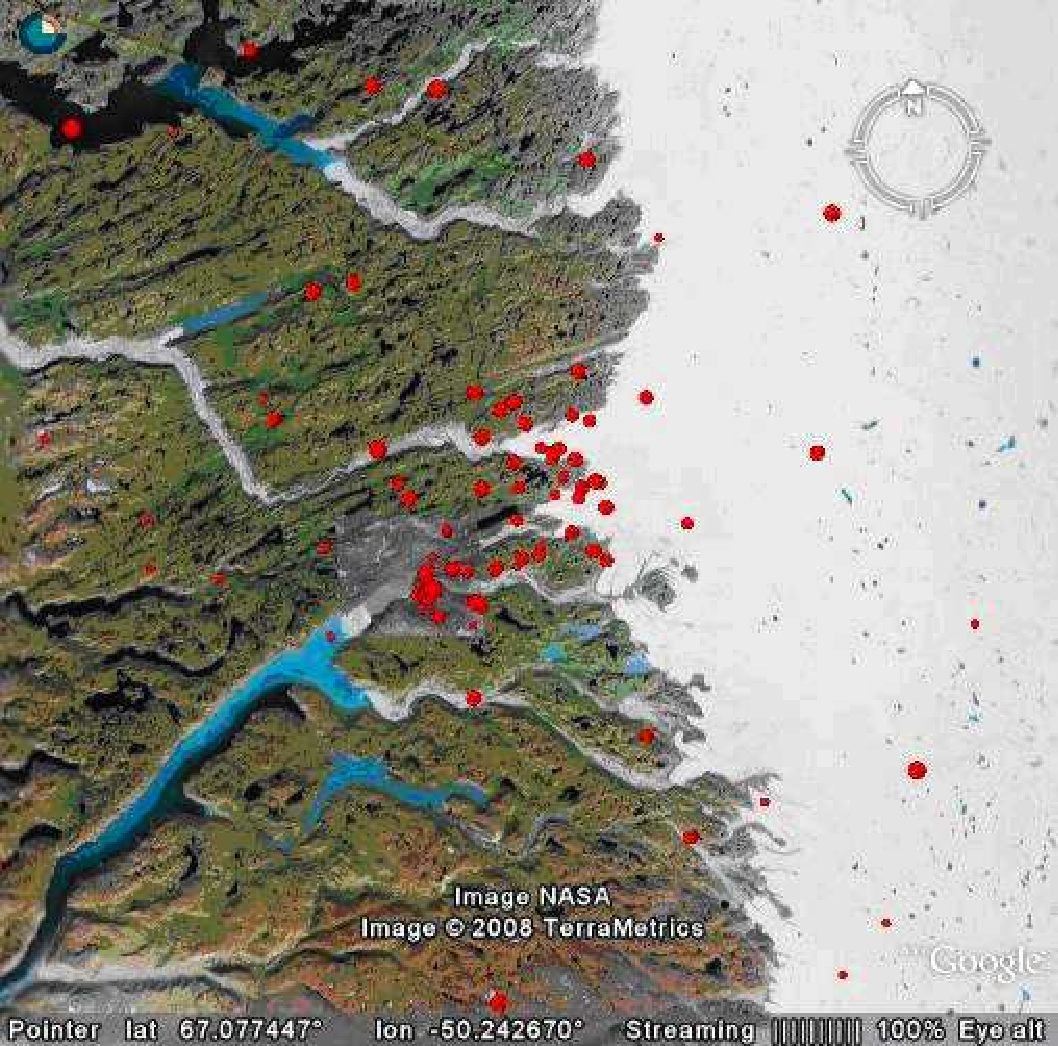
\includegraphics[width=0.9\linewidth]{fig/fig34}}
\caption{A map can be saved as raster file (File-Save-Save Image).}
%\label{fig:}
\end{figure}

GMAP parameters added to \texttt{SEISAN.DEF}: 
Icon used for earthquake, explosion, probable explosion and other events: 

\begin{small}
\verbatiminput{include/gmap.par.1}
\end{small}

Events with magnitude smaller than GMAP\_ICON\_MSIZE will be plottet with size of GMAP\_ICON\_MSIZE: 

\begin{small}
\verbatiminput{include/gmap.par.2}
\end{small}

The scale of the earthquake icons is give by GMAP\_ICON\_XSIZE*magnitude**GMAP\_ICON\_YSIZE: 

\begin{small}
\verbatiminput{include/gmap.par.3}
\end{small}

The scale of other events is furthermore multiplied by 2 Text can be added to the KML file, see this example, note the text must be placed from character no 41 to no 120: 

\begin{small}
\verbatiminput{include/gmap.par.4}
\end{small}

\textbf{GMAP -help:}

\begin{small}
\verbatiminput{include/gmap.help}
\end{small}

\subsubsection{The automatic GMAP}
\index{GMAP automatic} 

The automatic GMAP, is executed by the HYP program, when e.g. an event is located in EEV.

\begin{figure}
\htmlimage{scale=2.0}
\centerline{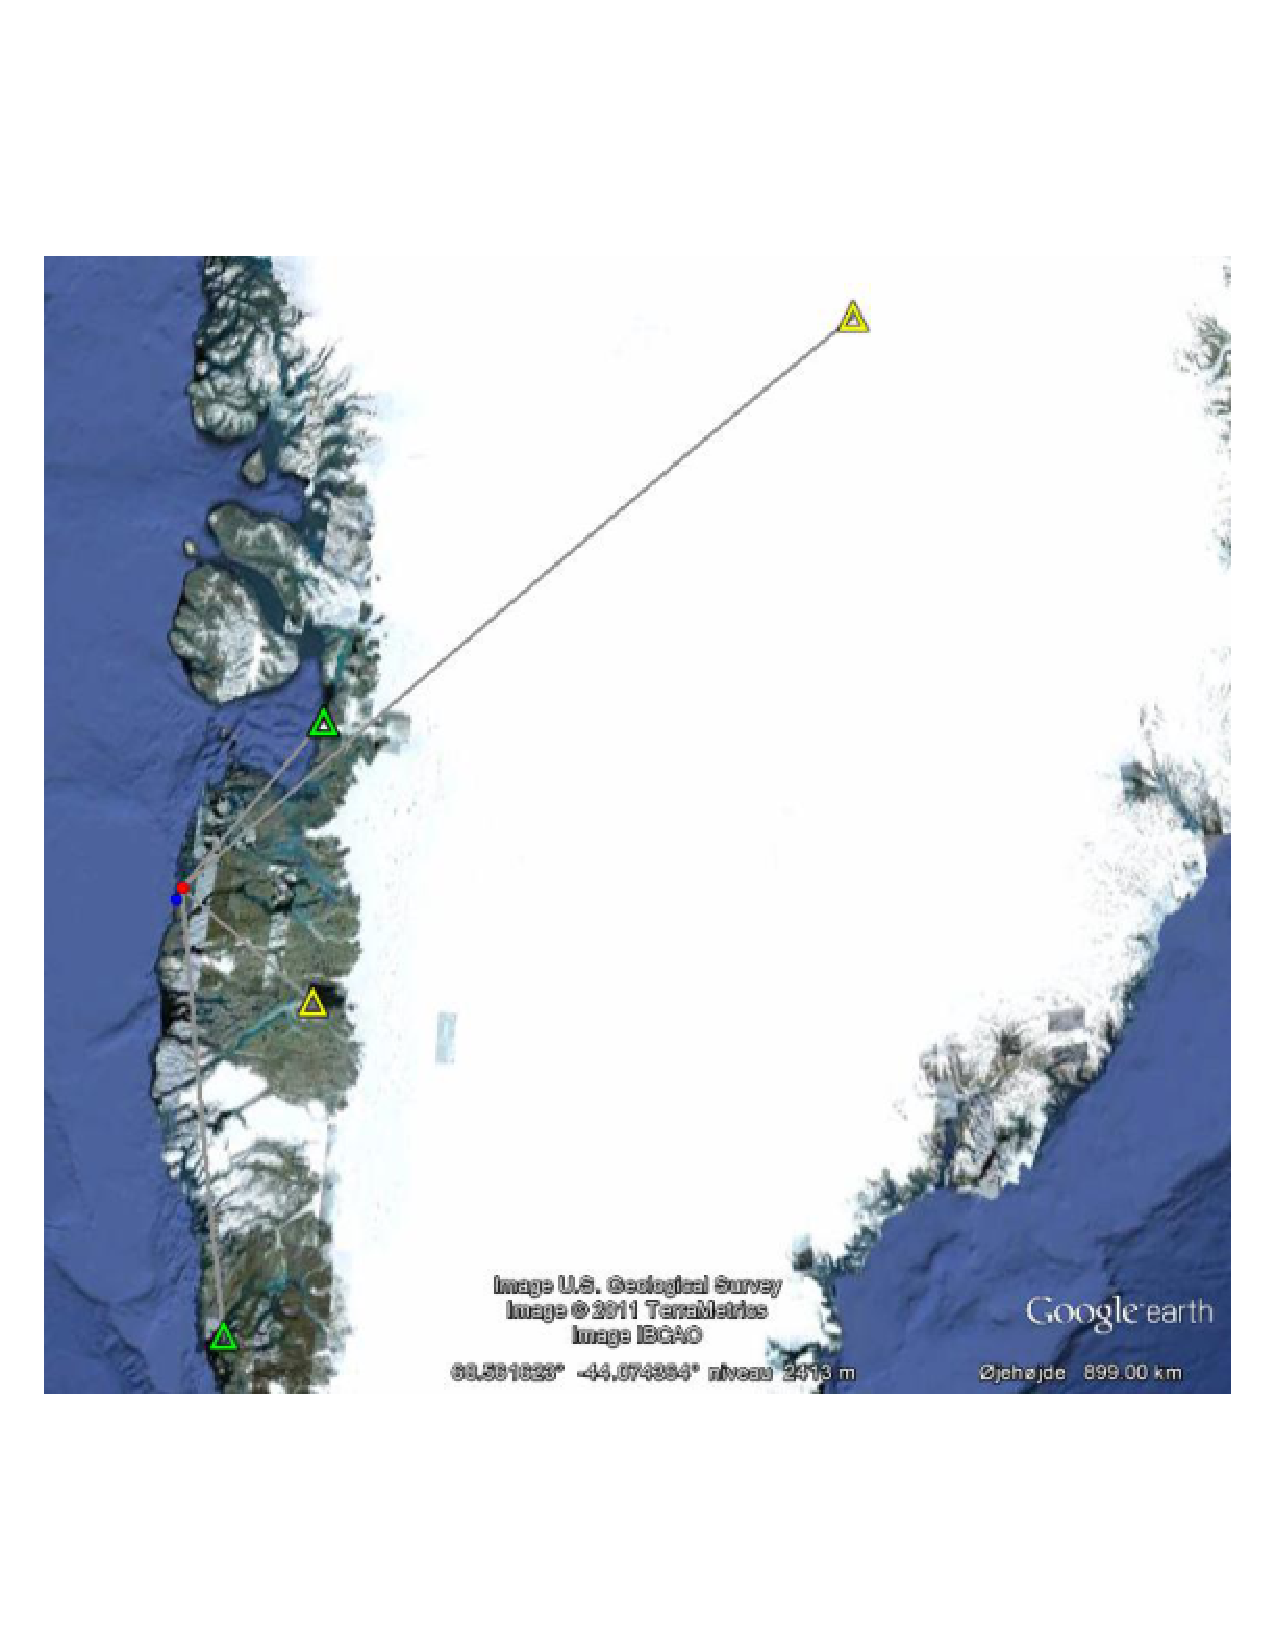
\includegraphics[width=0.9\linewidth]{fig/gmap-cur-kml}}
\caption{Example of automatic mapping with gmap. Earthquake in 
West Greenland. 
Blue dot is the old location and the red dot is the current location.
Green and yellow stations are stations with good and ok residuals, respectively.}
\label{fig:gmap.cur.kml}
\end{figure}

Start EEV and locate an event. In the directory a new file \texttt{gmap.cur.kml} 
will appear, this file can be opened with Google Earth and it will show 
the location of the current event and the used stations and the raypaths.

The color of the stations is given by the travel time residual as green, yellow or red,
for: residuals$<0.5s$, $0.5s=<$residual$=<1,5s$ or residual$>1.5s$, respectively.

To enable the automatic generation of Google Earth input files, add these parameters to your \texttt{SEISAN.DEF} file:

\begin{small}
\verbatiminput{include/gmap.par.5}
\end{small}

You can change the parameters to adjust the output file \texttt{gmap.cur.kml} for your system, see definition here \ref{ref:gmap.par}.

Inorder to run the display in a realtime mode, you must have an other KML file that makes Google Earth reload the \texttt{gmap.cur.kml} file at short intervals.
Such file could look like:

\begin{small}
\verbatiminput{include/gmap-automatic.kml}
\end{small}

In this example the \texttt{gmap.cur.kml} file is reloaded every 3 second from a local 
\texttt{C:\textbackslash seismo\textbackslash WOR} directory on a windows pc. 
And below is an other KML file is reloaded at 60min intervals from the Internet.

The above file is named \texttt{gmap-automatic.kml} and is found in the DAT directory.




\subsection{SEIS2VIEWER, Plotting hypocentres in 3D}
\label{subs:seis2viewer}
\label{page:seis2viewer}

The program is written by \textbf{Ruben Soares Lu\'is} (ruben.so.luis@gmail.com) and use 
the SeismicityViewer50 program by \textbf{Anthony Lomax}. To program has been aliased to smap.

\index{SEIS2VIEWER}

\textbf{Overview}

seis2viewer is a wrapper for the application SeismicityViewer, developed by Anthony Lomax for rapid mapping of seismic events. SeismicityViewer displays hypocenter locations in 3D as well as station locations and P/S residuals. Geographic and geologic features can also be displayed as well as focal mechanisms. Please find details here:\newline
\url{http://alomax.free.fr/seismicity/}

seis2viewer has been created to take information from a nordic file from Seisan and convert it in a format usable by SeismicityViewer 5.0 (NLLoc Format). It automatically launches Seismicity Viewer, generating a set of files required for its operation.

In its current version, seis2viewer allows the visualization of hypocenters and magnitudes in SeismicityViewer 5.0. Other information, such as station locations, P and S residuals, etc. is not displayed.


\textbf{Installation and Configuration}

\begin{enumerate}
\item[1:] \textbf{Configuration Files:}

\begin{itemize}
\item \texttt{seis2viewer.def} (mandatory): seis2viewer uses a \textbf{single} configuration file: \texttt{seis2viewer.def}, which may contain references to other files containing information on maps, elevation, localities, etc. The file \texttt{seis2viewer.def} is actually passed directly to Seismicity Viewer adding only a reference to an automatically created file. This operation is transparent to the user. As such, the configurations can be obtained from the Seismicity Viewer 5.0 website: \url{http://alomax.free.fr/seismicity/}
\item Other files: \texttt{seis2viewer.def} may reference other files containing map information, elevation data, locality names, etc. These files should follow the definitions presented in the Seismicity Viewer 5.0 website.
\end{itemize}


\item[2:] \textbf{Installation}

seis2viewer is distributed as a single .jar file (\texttt{seis2viewer.jar}), containing all the necessary classes to work, including Seismicity Viewer 5.0. This file should be placed in the PRO directory of seisan.
To facilitate the usage of seis2viewer, the administrator should create an executable script file to call seis2viewer. As an example, the executable script should contain the following line:

\begin{verbatim}
java -jar $SEISAN_TOP/PRO/seis2viewer.jar $1        (for unix/linux)
java -jar %SEISAN_TOP%/PRO/seis2viewer.jar %1%      (for windows)
\end{verbatim}

The configuration file, \texttt{seis2viewer.def}, and any other required files should be placed in the DAT directory of seisan. Alternatively, the user may have its configurations on the working directory.

\item[2:] \textbf{Automatically Generated Files}
seis2viewer generates a set of files to be used by Seismicity Viewer 5.0. Although these files are, in principle, irrelevant to the user, it is nevertheless important to mention them for reference purposes.

\begin{itemize}
\item \texttt{seismicitydefaults}: This is the default configuration file for Seismicity Viewer. It contains a reference to the converted events file, \texttt{seis2viewer.hyp}.
\item \texttt{seis2viewer.hyp}: This file contains a translation of the event file selected by the user for visualization in NonLinLoc format, appropriate for Seismicity Viewer.
\item \texttt{seis2viewer.hdr}: This is an automatically generated grid file for the area surrounding the events to be visualized. It is only created if the maximum distance in longitude or latitude between events is less than 20 degrees.
\end{itemize}

\end{enumerate}

\textbf{Usage}

seis2viewer can be used directly with a nordic file containing one or more events (e.g. \texttt{select.out}) as:

\begin{verbatim}
java -jar %SEISAN_TOP%/PRO/seis2viewer.jar select.out    (windows)
java -jar $SEISAN_TOP/PRO/seis2viewer.jar select.out     (unix/linux)
\end{verbatim}

or, if the executable script has been created, as (assuming the script is called '\texttt{smap}')\newline
\texttt{smap select.out}\newline
seis2viewer can also be called directly from eev, as an external program, using the prefix 'o' as:\newline
\texttt{osmap}\newline
In this case, smap will try to find the file eev.cur.out, which is automatically generated by eev and contains a reference to the event that is currently under work.


%SEIS2VIEWER can run in two modes: 
%
%One earthquake from EEV:\newline
%Type \texttt{osmap eev.cur.sfile} in EEV.
%
%Many earthquakes:\newline
%Type e.g. \texttt{smap collect.out} to 
%plot many earthquakes from file collect.out. Note if the earthquakes cover a large area 
%they will be shown in Global mode, if the earthquakes 
%cover a small area they will be shown in Local mode.
%The depth of the earthquakes can only be shown in Local mode.
%
\begin{figure}
\htmlimage{scale=2.0}
\centerline{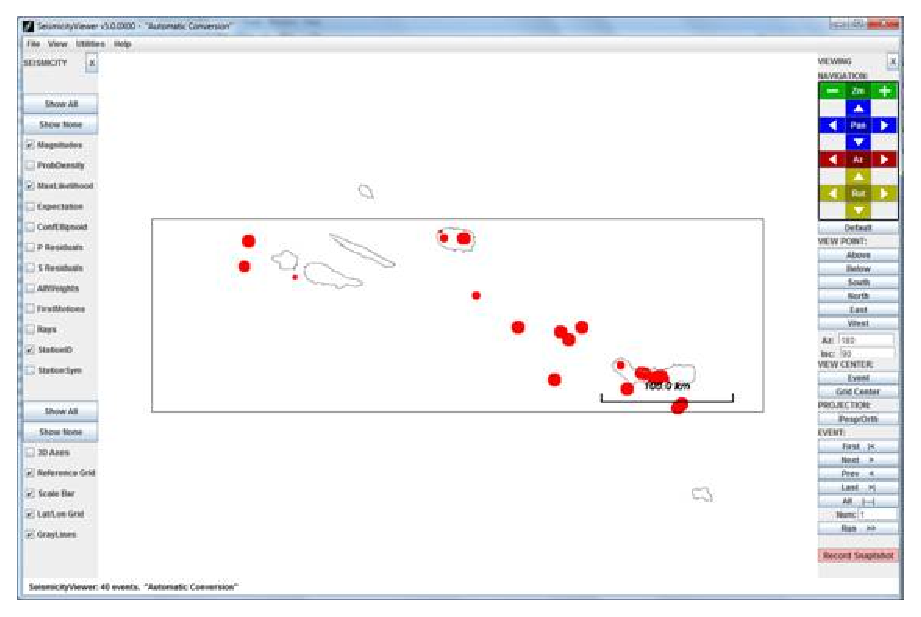
\includegraphics[width=0.9\linewidth]{fig/seis2viewer}}
\caption{Epicenter map by SEIS2VIEWER.}
\label{fig:seis2viewer}
\end{figure}

%SEIS2VIEWER uses the following files from the 
%\textbf{DAT} folder:
%\textbf{seis2viewer.def}, and one of the coast line files 
%\textbf{azores.xyz} or
%\textbf{europe.xyz}.
%Note: it seesm like the file azores.xyz is only found if in working directory.
%You can construct your own coast line files, e.g. using GMT in unix by:
%
%\begin{verbatim}
%pscoast -M -W1 -P -R-60.00/50.0/60/78r -JT-40/10 -Dl > greenland.xy
%awk '{print $0" 0"}' greenland.xy > greenland.tmp
%grep -v "# Data" greenland.tmp | sed 's/>\([a-z]*\).*/> GMT_LONLATELEV_M/' > greenland.xyz
%\end{verbatim}





\section{Searching in the database, SELECT}
\label{sect:select}
\index{SELECT}
\index{Searching in the data base}

Whenever selective search and extraction is wanted SELECT is used. The program can run on the CAT database, single CAT files (Nordic or Nordic compact) or the S-file data base. The output file, \index{Select.out}\texttt{select.out}, will also be in Nordic format. Since the input CAT database can contain both normal and compact files, the output will always be a normal file with blank lines between events. If however the input is one compact file, the output will also be a compact file. 
Note: If SELECT is used on the CAT database (normal operation), you need to UPDATE your S-file database in order to transfer changes from the S-files to the CAT database. 
Select can work with input in 3 different ways: 
\begin{enumerate}
\item 
The user is asked for selections 
\item 
The selection parameters are in a file 
\item 
Parameters are given on the prompt line 
\end{enumerate}
The program is started by typing SELECT (parameters from screen), 
SELECT `input file' (parameters from input file) or SELECT -options. 
A typical user interactive run is shown below. Comments following ! 

\verbatiminput{include/select.run}

Note above, that the second time the menu is shown, the choice of magnitude limits is shown.  For each CAT file in the catalog, the number of events in file, number of events selected from that file and the accumulated number are listed. The last file might not show the correct number of events in file since SELECT might stop before reading the whole file if the end time is in the middle of the file. If start time is blank, 1980 is used. The end time can also be blank, and 2015 is used. This option is useful when selection on whole data base or whole file. 
Input parameters: 

In the input database (or file) a time window must always be given. If no more selection is done, all data in time window is selected. Further selection can be done by choosing a number and giving parameters. The chosen parameters are then shown on the next parameter selection menu as shown above for magnitude. Parameters can be reentered. Parameters not entered will have no influence in the selection. If several parameters (numbered selections below) are entered, conditions for all must be true for the event to be selected. Within each numbered selection, usually only one of the entered conditions must be fulfilled for the event to be selected. If e.g. Ml and Mb are selected, events, which have either magnitude, will be selected. When no more parameters are desired, press enter. 
\begin{enumerate}
\item 
- Fault Plane Solution \newline
Selects events with a fault plane solution (F- line in S-file). 
%\textcolor{red}{jh-change: 
There will also be the question: "Give quality, e.g. A or ABC, enter for all", in this way different qualities can be selected.
\item 
- Earthquake Felt\newline
\index{Event felt, select for}Events felt indicated by a type 2 line 
\item 
- Magnitude Type(s) \newline
Normally, all magnitudes for one event are searched to see if any 
magnitude fits the selection criteria. With option 3 it is possible 
to use one or a combination of magnitude types e.g. L and B. If 
\index{Magnitudes without type}magnitudes without type are to be 
selected, use underscore ``\_'' for magnitude type. If there is no 
magnitude in the first magnitude position, chose ``N'' for one of the 
magnitude types to be able to select the other 2 magnitudes on the 
line. 
%\textcolor{red}{jh-change: fixed new mags here}
Magnitude types are: C: \index{Coda magnitude}Coda magnitude, 
L: \index{Local magnitude}Local magnitude, b: \index{mb}mb, B: \index{mB}mB, s: 
\index{Ms}Ms, S: \index{MS}MB and W: Moment magnitude. N: Find events with no 
magnitude in first position. An event is selected if any one of the 
types of magntudes are found. Magnitudes are only searched on first 
header line unless ``Use all header lines is set''.
\item 
- Distance ID(s)                           \newline
Restricting the search to be for one or a combination of the distance id's L, R and D. 
\item 
- Event ID(s)                              \newline
Restricting the search to one or a combination of event id's, e.g. E and V for explosion and volcanic events. The letters used for selection are not limited to the examples shown above, they are however the ones used currently. It is thus e.g. possibly to label events as X for \index{Unknown type}unknown type (column 23 in header line) and then later on select out all those events by specifying X for event ID. For the 3 questions about types, up to 5 letters can be used. The currently used codes are: \index{Distance id} E: Explo\index{Explosion}sion, P: \index{Probable explosion}Probable explosion, V: \index{Volcanic}Volcanic, S: \index{Sonic boom}Sonic boom, Q: Earthquakes which is equivalent to blank for type. However, if blank is selected, all event types are selected, while if Q is used as input, only events with no ID or Q ID are selected. So if all earthquakes and volcanic event are to be selected, use QV. Without the Q, only volcanic events are selected. Selection is made if either one of criteria is met. 
\item 
- Magnitude Limits \newline
Range of magnitudes to select.  Note that if no magnitude type is given, the extreme of all magnitude types reported is used. Magnitudes are only searched on first header line unless \"Use all header lines is set\". 
\item 
- Latitude Limits \newline
Range of latitude. NOTE: If no latitude or longitude values are chosen, SELECT will include an event even when it is not located if the remaining criteria are OK. If it is required that only located events are searched for, enter at least one value like an upper latitude limit of 95. 
\item 
- Longitude Limits\newline
Range of longitude. 
\item 
- Depth Limits\index{Depth, select for}\newline
Range of depths. 
\item 
- RMS Limits\newline
Range of rms travel time residuals. 
\item 
\index{Polarity, select for}
- Number of Stations Limits \newline
Range of number of stations. 
\item 
- Hypocenter Errors Latitude Limits \newline
Range of hypocenter latitude errors. Works only if error line (E-type) is present in S-file. Currently error lines are generated by HYP and the ISC conversion program ISCNOR. There should only be one error line in file associated with the prime solution in first header line. However, if more than one error line is present, all are checked and if one fulfills the selection criteria, the event can be selected.\index{Errors in hypocenter}\index{Selection on errors}
\item 
- Hypocenter Errors Longitude Limits, See 12. 
\item 
- Hypocenter Errors Depth Limits, See 12. 
\item 
- Minimum Number of Polarities, only P-phases are used \newline
Counts all polarities, useful to find potential events for fault plane solutions. 
\item 
- Hypocenter Agencies \newline
Selects events only with given hypocenter agencies as indicated on header line. 
\item 
- Magnitude Agencies\newline
\index{Magnitude, select for}\index{Agency, select for}Select only events with given magnitude agencies as indicated on header line. Magnitudes are only searched on first header line unless \"Use all header lines is set\". 
\item 
- Station Codes, components, distance range and phase\index{Distance range, select for}\index{Select for phase}\index{Phase, select in data base}\newline
Selects only events with given stations, component, distance range and phase. A formatted help line comes up for selecting items. Any one or a combination can be selected, however, a station code  
%\textcolor{red}{jh-change: 
or component code 
must be selected. The distance can be hypocentral or epicentral. Distances are integers right justified. A special option is to make a file used for input to CODAQ. The station name CODAQ is selcted and all stations present within the specified distance range are seleted and the output is written in file index.codaq which then contains the event-station combinations used as input to CODAQ. 
\index{CODAQ, select events}
\index{index.codaq}
\item 
- Polygon \newline
Selects events within a given polygon of at least 3 latitude-longitude pairs.\index{Polygon, select}
\item 
- Use all header lines\newline
All header lines are searched for relevant information 
\item 
- Look for waveform file names\index{Waveform files}\newline
Search the database for particular waveform files, input can use a fraction of file name or * for any name. No wildcards can be used in the string so e.g. ASK* will select all due to the *. Use just ASK in this case to select all filenames with the string ASK. 
\item 
- Gap range\index{Gap range, select for}\newline
The range of gap as given on the E-line (normally 2. header line). Only hypocenters calculated with SEISAN version 7.0 have gap. 
\item 
- Phase \newline
Look for events with particular phases. Up to 6, 4 character phase names can be selected. The event is selected if at least one of the phases is present for the event. For a more selective selection based on phase, see option 18. 
\item 
- Volcanic subclasses \newline
Search for events of given subclasses given by up to 10 codes. Any code can be given, however, normally they will be as defined in VOLCANO.DEF. The program searches for lines starting with `VOLC MAIN'. 
\end{enumerate}

Historical data: When working with historical data, it can be useful to work with catalogs of several centuries. The century is available in the Nordic Format, so catalogs can go back to year 0. 
Output: 

\texttt{select.out}: A CAT-file or compact file (depending on input) of selected events.  

\texttt{index.out}: 
\index{index.out}
A list of event id's of selected events can be used with EEV or other programs accepting inde\index{Index file}x files. This could be used e.g. to work on only distant events in the database by first selecting all distant events and then working with these directly in the database using command EEV index.out. Index files can have any name (must contain a `.') so different subsets can be available with different index files.  

\texttt{Waveform\_names.out}: 
\index{Waveform\_names.out}
A list of corresponding waveform files. It is mainly 
intended for copying to or from tape specific waveform files.  It has the format of the \texttt{filenr.lis} files and can be used directly with e.g. MULPLT. See also program get\_wav for selecting waveform files from the database. 

\texttt{select.inp}\index{select.inp}: A file with all the parameters used for the run. The file can be renamed, edited and used as input for select. This is particularly an advantage if a complex set of selection parameters are used and the selection is wanted again with just a small change. An example file is shown below 
\verbatiminput{include/select.inp}

Note: The TT at STAT line indicates that all stations must be present (True) and hypocentral distance 
is used (True) 

Select with input from the prompt line 

This option is particular useful when using select with automated operations and has been made specifically to deal with extracting data out of the data bases using WEB based software. This option do not have all of the above options. The following are implemented: 

\begin{tabular}{|lp{8cm}|}
\hline
-base : & 5 letter data base \index{WEB options} \\
\hline
-seisweb: & if set, WEB output parameters  \\
\hline
-time : & time interval (2 variables)  \\
\hline
-web\_out: & complete path to where data is placed, only \newline
active if seisweb set. 3 files are made: \newline
\begin{tabular}{ll}
\hline
\texttt{web\_out.id} : & id's, like \texttt{index.out} without \\
\texttt{web\_out.all} : & like \texttt{select.out} \\
\texttt{web\_out.head} : & header lines  \\
\end{tabular} 
\\
\hline
-area : & lat-lon grid, minlat,maxlat,minlon,maxlon  \\
\hline
-depth : & depth range, mindepth,maxdepth \\
\hline
-mag : & magnitude range, minmag,maxmag \\
\hline
-nstat : & range of number of stations, min,max \\
\hline
-gap : & range of gap, min,max \\
\hline
-rms : & range of rms, min,max \\
\hline
-magtypes : & up to 5 mag types, one string, e.g L \\
\hline
-disttype : & distance type, e.g D \\
\hline
-eventtype : & event type, e.g. E \\
\hline
\end{tabular}

Problems: \index{Problem, select}An event might be found and listed in 
\texttt{index.out}, but when looking for it with EEV, it is not there. 
This can happen if an event has been deleted with EEV and no UPDATE 
has been made, so that the event is still present in the CAT part of the database. 


\subsection{Searching for text string in nordic files, SELECTC}
\label{page:selectc.jar}
\index{SELECTC}
\index{Searching for text string in nordic files}

The command SELECTC is used to search for text stings in nordic files 
like \texttt{collect.out} or \texttt{select.out}. Events with the maching 
text string is listed in the output file 
\texttt{selectc.out}. 
The program is written by \textbf{Ruben Soares Lu\'is}.
Below is an example :

\verbatiminput{include/selectc.run}




\section{Extracting events from the database, COLLECT}
\label{sect:collect}
\index{Extracting events from the database}\index{COLLECT}

The command COLLECT is used for collecting many event files from the database \index{S-file}S-files into a single file. This may be sp\index{SPLIT}lit into individual event files later using SPLIT. The file can be used for exchanging data with other agencies or be used with the epicenter plotting program. The questions are: 

\verbatiminput{include/collect.run}

%\textcolor{red}{jh-change: 
If a local data base is input, default start time is 1980 and default end time 2015. In this way it is fast to collect all data from a local data base. 
At the end, the program will give statistics of collected data, and file name. For getting data out of the database represented by the monthly CAT files, use SELECT. If an update has been made, SELECT will always be the fastest program to use. COLLECT and SELECT are the only programs that can make a CAT file from the individual S-files. \index{S-files, collecting}Program input can also be on the prompt line, below is an example: 

\texttt{collect -start\_time 19910912 -end\_time 19911015 -base\_name BER -compact}

This means that a CAT-file (default) is collected from BER and is written in compact format (-compact has no arguments). The time interval is between 19910912 and 19911015. Only start\_time is required, the other arguments are optional. The syntax is:  -"keyword" value -"keyword" value etc. 




\section{Inserting events into the database, SPLIT}
\label{sect:split}

\index{Inserting events in the database}\index{SPLIT} The program splits up a \index{Multiple event S-file}multiple event S-file in Nordic format (usually made by COLLECT or NEWEVE) or compact file to single files in the database or in the users own directory. Type SPLIT to start program and questions are: 

\verbatiminput{include/split.run}

In the above example, there was already an event in the database with the same file name and therefore the same id. It is up to the user to decide if this is the same event in which case it should be ignored or if it is a new event which happens to have the same id (start time or origin time to the same second and same event type). In case of a new event, a new id with one second different will be tried. Sometimes it can be desirable to overwrite the whole database event by event. If e.g. a station code is wrong in all events, this can be corrected by making a coll\index{Duplicate ID}\index{Event, duplicate ID}ect to extract all events, edit the \texttt{collect.out} file using a global substitute, and finally use split to put the events back in. In that case the option of overwriting all should be chosen. 

\index{Compact file}Compact files can also be split up. Since this is unusual to do, the user will be prompted 2 times to confirm the split up. Since there is no ID line in a compact file, the database name will be generated from the header time. This option to be able to split up compact files has been made to facilitate work with seismic catalogs where it is often desirable to be able to access individual events even when no readings are available.\index{Catalog work} 



\section{Updating final locations in database, UPDATE and UPD} 
\label{sect:update-upd}

\textbf{UPDATE}

Both the \index{Monthly epicenter files}
monthly epicenter files in 
\textbackslash SEISMO\textbackslash REA\textbackslash BER\_\_\textbackslash CAT 
and the \index{Updated S-files}updated S-files are generated with program 
UPDATE which is a special version of HYP. Type UPDATE to start the 
program and there will be questions about time period and database. 
The program will also ask for \index{Operator ID}operator ID (4 chars), 
which is stored in the updated \index{Log file}log file and the S-file, see below. \newline
By updating, both the S-files and the CAT-files in the CAT-directory 
are updated. The reason for updating both at the same time is to ensure 
that there is a correspondence between the two. \index{UPDATE} 

The program will go through as many months as specified by the user. When the program is running, one line will be printed out for each event. The S-files will be overwritten with the updated location, residuals etc. At the same time, a monthly CAT file is created in the CAT directory containing all events, also events not located. If a monthly file is already present, it is overwritten. 

Update can also work on a local database. The S-files are updated as described above. Since there is no CAT database, the Update program makes a CAT file in the local directory called hyp.cat\index{Hyp.cat}\index{Local database, update} with events in chronological order. 

At this time, an S-file might contain several old ID-lines which in an append process have \index{Delete ID-line}been converted to comment lines. These are deleted when doing an update. The remaining \index{ID-line}ID-line is updated with the action UPD, the operator ID and the time. At the same time, all the error lines are deleted and only the one belonging to the prime location is kept. 

The update process can also change all S-file names according to the origin time and the ID's are changed correspondingly. This is done in order for the database to be in \index{Chronological order}chronological order according to origin time and not the more random times used when the events were first registered into the database. Even if the event is marked not to be located with a * in header line column 45, the ID will still be updated (same for program UPD). Like with the SPLIT program, if two events of the same type (L, R or D) have the same origin time to the second, one second is added to the file name part indicating seconds (see also section 6.6). The event will also be in chronological order in the CAT database. 

*****VERY IMPORTANT ****** 

The first time an update is done, the S-files get a new name according to the origin time now calculated and the internal ID is changed accordingly. The ID is then locked indicated by an L in column 76 of the ID line. For all future updates, by default, the ID will remain the same, the S-file name will also be the same irrespective if the origin time changes. This is VERY important in case data is taken out of the database for some special analysis and then put back in to overwrite the original data. If the ID is the same, the correct event will be replaced. Optionally, Update can make a new ID each time the program runs (not recommended). It mig\index{Chronological order}\index{ID, lock}\index{Lock ID}ht be necessary sometimes to allow this in case the events are no longer in chronological order according to origin time (e.g. a teleseismic event is put in with the ID corresponding to the recording time, when located, the origin time is many minutes before and it will appear too late in the database). However, this is rarely a problem after the first location is done and it is recommended to use the default option of locking the ID. 

NOTE: When an update takes place, the old location, magnitudes 
(except 3. if a different agency from the default agency), residuals 
etc are removed. If an event cannot be located, the old location etc 
is lost. This is intentional since the updated database should represent 
the data available. If a location should be retained, special flags 
must be set, see section \ref{sect:hypocenter}, 
``Fixing location'' (a `*' in column 45 in header line). 

In order to keep track of how and when the database has been updated, 
every run of UPDATE\index{UPDATE} creates a \index{Log file}log file 
of the update process. This file is located in a subdirectory of the 
database directory (default BER\_\_). If e.g. updating REA, the 
logfiles will be in ../REA/BER\_\_/LOG/ (unix). Filenames are similar 
to S-files. Below is an example of a logfile with name 
\texttt{01-0000-00L.S199606}:


\begin{verbatim}
1996 06 kk   99-09-08 14:30 03-1955-35D. 25-0337-29L.     6 
1996 06 jh   98-09-08 14:29 03-1955-40D. 25-0337-31L.     5 
\end{verbatim}

The content is as follows: date and time of file updated, operator ID, time of update, event id of first and last event of the month, number of events for month. The example above shows that June 96 has been updated 2 times, the last time on September 10, 1999. For each update, one line is added to the top of the file, so the update history is saved. 

Note: If the command UPDATE is used from EEV, only one S-file is 
updated (name stays the same), and a general update should be made. \newline
UPDATE recalculate moments if distances (or depths) change, however 
it does not change the Vp or Vs velocities used if a change is made 
in MULPLT.DEF. \index{Update spectral parameters}
\index{Spectral parameters, update}\index{Update without relocation}

\index{Problem, UPDATE}
Problem: If UPDATE crash, there will not be a correspondence between 
S-files and the CAT data base: Redo UPDATE. 

\textbf{UPD}
 
The command \index{UPD}UPD is very similar to the UPDATE command, however there is no modification of the S-file except the ID line. The program is used to simply move single S-files into the monthly CAT-files without relocating. It is mainly used to manipulate database events already processed. E. g. if ISC data a available and it is desirable to have it in individual files to be able to use EEV, the same data can then be copied into the CAT part of the database using UPD without modifying the original solutions. The data must be in the CAT part of the database in order for SELECT to work fast. K\index{Problem UPD}NOWN BUG: On Sun OS, it seems that UPD can only operate on up to a 4 year time period. \index{Problem, UPD} 

\section{Using \texttt{filenr.lis}, DIRF and DELF}
\label{sect:dirf} 
\index{DIRF} 

\textbf{DIRF}

The DIRF command is a useful program for making a file with a numbered list of files from a directory. The command makes a file with file name \index{FILENR.LIS}\texttt{filenr.lis} e.g. when working with many waveform files with long names, a DIRF is first made, and subsequent programs then get file names from \texttt{filenr.lis}, either by using the whole list, or just a given number. This is handled with routine filename (in LIB). Below are some examples of using DIRF with SEISAN data files. 

\begin{boxedverbatim}
 dirf 9101-10* 
 #  1  9101-10-0915-15S.KMY_01
 #  2  9101-10-1510-55S.N2F_08
 #  3  9101-10-2333-44S.N3F_06 


 dirf 9101-10-0915-15S.KMY_01 9101-10-2333-44S.N3F_06          (Unix only) 

 #  1  9101-10-0915-15S.KMY_01
 #  2  9101-10-2333-44S.N3F_06 

\end{boxedverbatim}

The \index{Wildcard}wildcard `*' above indicates that all files from 
the 10'th is wanted. Many programs use the same subroutine to get 
the file name from \texttt{filenr.lis}. This means that most programs using 
\texttt{filenr.lis} assume that if a name given is less than or equal to 4 
characters, it is a number so file names less than 5 characters cannot 
be used when the program asks for ``Filename or number''.\index{Problem, filenr.lis} 

\textbf{DELF}

DELF\index{DELF} is a simple program that allows the user to delete 
a file that is listed in a \texttt{filenr.lis} file or another index file. 
First run DIRF to list the files that you want to delete. Then start 
DELF and choose the number of the file to delete, `?' shows the 
contents of \texttt{filenr.lis}. In addition, DELF also has an option to 
delete all the files in the \texttt{filenr.lis} or index file. This is a 
useful option if selected files in a data has to be deleted. If e.g. 
all S-files from a particular agency has to be removed, run SELECT 
first and then DELF.\index{Delete many S-files} 

\section{Making a bulletin, BUL}
\index{Bulletin}\index{BUL} 

The bulletin program BUL is intended for writing seismic bulletins 
in a nice format. The output is written to a PostScript file. 

Input files: 

\begin{enumerate}
\item
A monthly data file: This file can be made by COLLECT or SELECT 
\item
\index{BUL.INP}\texttt{BUL.INP} : This file must be in DAT or in the local directory. 
In this file the layout of the front pages are decided, as well as 
the font selection for the main bulletin. There are ample comments 
in the file on how the commands are written. 
\end{enumerate}

Some special format features: 

Type 3 line: If the first 5 columns in a type 3 line are:" Bul:", then the rest of the line is interpreted as text line that is written in the bulletin. In this way comments to certain earthquakes can be written into the bulletin. Type 2 line: Maximum intensity and casualty/damage reports are included in the bulletin if found in the S-file. 

How to run the program: 

Type \texttt{bul -h} this gives you a list of the different options like this:

\begin{tabular}{ll}
       Options: & \\
-frontpage: & Only frontages are printed. \\
-nofrontpage: & No frontages are printed. \\
-onlyhypo: & Only hypocenter solutions are printed. \\
-minmag x.x : & Only hypocenter solutions with magnitude than the requested are printed.\\
\end{tabular}{ll}
 
The last option may be used in cases where the number of earthquakes is very high, so that it is preferable to report phases only for events above a given magnitude. 

You can also run the program without any options, in which case the default values used are:  

\begin{itemize}
\item[i)]
All phases are reported. 
\item[ii)]
Front pages are printed. 
\end{itemize}

You will always be asked for the name of the S-file. 

Output file: 

The output file is called \index{Bul.ps}\texttt{bul.ps} and is a PostScript 
file that you can print. Optionally, a limited number of pages can 
be selected from the \texttt{bul.ps} file for printing. The header page is 
still included and the page numbers correspond to the original page numbers. 

\section{Reports and statistics}

SEISAN has several programs for extracting and writing out data for plotting or printing statistics, most of which will be listed in this section. 

\textbf{Report}
\index{REPORT}

The program extracts parameter data from all header lines in a CAT 
file and rearranges the data in a table. In additions, there is an 
option to rearrange order and location of magnitudes on the header 
line. Below is an example of a run where the input CAT file is called 
\texttt{collect.out} :

\verbatiminput{include/report.run}

The \texttt{report.inp} is a file with the choices used. Report can use that 
file (or a file with the same format and a different name) as second argument: 

\texttt{report collect.out report.inp} \index{Report.inp} 

in order to use a fixed set of choices. 

Content of \texttt{report.out}

\verbatiminput{include/report.out}

\index{Report.out}\index{Report\_n.out}
The file \texttt{report\_n.out} contains the input data with the only difference 
that the magnitudes have been moved around on the header line. This 
can be practical for later plotting with EPIMAP. If no magnitude 
selection has been made, the magnitudes will come in the order Mc, 
Ml and Mb. If no magnitude of that type is available, the output 
field is blank. The magnitude selected 
\index{MAG}\index{EPIMAP}
is the first to occur of the corresponding type. If other magnitudes 
are to be selected, numbers can be used to select any 3 magnitudes 
in any order. If it is important to select magnitudes by agency 
also, use program MAG.
%\textcolor{red}{jh-change:
REPORT can also give a numbered output by adding the second or third argument \verb|-n|.
\index{Order of magnitudes}\index{Magnitude order}\index{Spectral parameters} 

\textbf{NORHEAD, making a compact Nordic file from a Nordic file}

You must give arguments: First is input file, optional second is 
output file, if an optional second or third argument is -mag, 
magnitudes from following header lines are moved up to empty 
magnitude spaces on first line. The program was earlier called 
COMPACT (version 7.2 and earlier).
\index{Magnitude, move from 2 header to first} 

\textbf{STATIS, statistics of databases}
\index{STATIS}

This is a simple program for making statistics of stations used in the database or in a file. The program will ask the following questions: \index{Statistics}\index{STATIS}\index{Earthquake statistics}

\begin{enumerate}
\item
Information about which stations should be searched for in the database. There are several options for entry: 
\begin{itemize}
\item[a:]
Give a filename with the stations listed one per line. The format is a5. The file name MUST have a '.' not to be confused with option (b) below. 
\item[b:]
%\textcolor{red}{jh-change: 
Give stations, one pr line, enter to finish, enter for def file statis.def
\item[c:]
Just make a return and the stations
%\textcolor{red}{jh-change: 
given in file statis.def will be used. The file has one station per line an dcan be located in either the working directory or DAT. 
\end{itemize}
\item
 Standard questions about base or filename and time interval 
\item
Question about counting all phases. This means counting the occurrence of a station for each phase for that particular station. This can give the total number of phases read at a particular station in a given time interval which can be more than the number of events. If not counting all phases, the program gives the number of events recorded at the station. 
\end{enumerate}

The output from the program could be as follows: 

\verbatiminput{include/statis.run}

The top part shows the event statistics by station. Local Ev is number of local events (readings if so specified above) (type L and R) at the station, Local S means number of local events ONLY recorded at that station, Distant E and distant S is the same for distant events (type D). The middle parts shows the number of waveform files NWAV from different networks NET as indicated by the first 3 letters of the waveform file name after the "." At the bottom is a summary statistics most of which should be self-explanatory. The information about ".. more than given stations" means that in addition to the stations searched for, the event had additional stations not used in the statistics. 

\textbf{CATSTAT}
\index{CATSTAT}

This program calculates the yearly, monthly and daily number of events from a given \index{Yearly number of events}earthquake catalog\index{Catalog work}ue and plots the results (written by \textbf{Mario Villagr\'an}). The input is a standard Nordic file containing only the header lines (compact file). The output is given in three different files with following default file names: \index{Earthquake statistics}\index{Statistics}\index{Monthly number of events}\index{Daily number of events}

\begin{tabular}{lp{8cm}}
\texttt{catyear.out} \index{Catyear.out}: & Output catalogue of the yearly number of events. This file contains two columns of data corresponding to year and the number of events. \\
\texttt{catmonth.out} \index{Catmonth.out}: & Output catalogue of the monthly number of events. This file contains three columns of data, corresponding to the year, month and the number of events, respectively. \\
\texttt{catday.out} \index{Catday.out}: & Output catalogue of the daily number of events. This file contains four columns of data corresponding to the year, month, day and the number of events, respectively. \\
\texttt{cathour.out} \index{Cathour.out}\index{Cathour.out}: & Hourly distribution of events within a day interval. \\
\end{tabular}

In addition, a series of files with gmt in name give similar output for use with gmtxy (only Unix). The output files can then be used for plotting the histograms for the desired time interval at yearly, monthly or daily intervals. If desired, the corresponding histograms can be plotted interactively on the screen or can be printed. Several other routine programs such as grapher, xyplot, gnuplot or GMT, etc., can also be used for this purpose. The general purpose of this program is to evaluate the catalogue completeness. When run for different magnitude intervals, one can detect the magnitude thresholds above which the catalogue can be considered complete. 

\textbf{SWARM, finding earthquake swarms}
\index{Swarm,seismic}\index{Swarm.out}\index{Swarm, identify}

The program is used to identify seismic swarms in a catalog. Input to the program is a CAT file with many events and some manually entered parameters. Output is identified swarms. The output file swarm.out contains all swarms organized as 'events'. In the header line is given the center for area identified and the 'magnitude' is the number of events in the area divided by 10. The rest of the line is information from first event in swarm.                                    

Principle of selection: 

The area is divided into a lat-lon grid. Around each grid point, there is a cell with radius small\_r. The program first checks the number of events in each cell for the whole catalog. It then checks each cell to 
find which has more than the minimum number of events to constitute a swarm under the condition that enough events are within the required time window. For each time window, with enough events, a swarm is declared so a swarm lasting e.g. twice the time window will be declared as two swarms. An additional condition is that the number of events is larger than the normalized background activity. The normalized activity is calculated as the activity in the large cell normalized for area to the small cell, and normalized in time to the window for the swarm. 

\textbf{STATSTAT, number of events per seismic station in catalog}
\index{STATSTAT} 

The program reads Nordic file input data and writes out text files giving the number of events per station. 

\textbf{LSQ}

A simple program to make and plot a least squares relation between 
two parameters. Input is from a file with two columns x and y. The 
program also makes an output used with GMT in order to make nice 
plots. The PostScript output  file is \texttt{lsq.eps} and the GMT file is 
\texttt{lsq\_gmt.out}. In order to produce the GMT plot (only Unix), use 
command \texttt{gmtxy lsq\_gmt.out}. 
\index{Least squares}\index{LSQ}\index{Lsq.eps}\index{Lsq\_gmt.out}\index{GMTXY} 

\section{Waveform file management tools}

This section describes the programs used for modifying and checking waveform files. The most important features are to add or subtract channels and modify headers. A special program in this group is GET\_WAV which checks data bases for availability of waveform files. New from version 7.1 is that SEISAN also can handle other waveform formats, however not all programs can work with all formats. This will be indicated with each program. The following programs are available: 

\begin{tabular}{lp{8cm}}
APPEND: & Append two or more waveform files following each other in time \\
AUTOREG: & Automatically register events \\
CONGAP: & Check completeness of continuous waveform database \\
CONNOI and EVANOI: & Compute noise power spectral density and evaluate out to produce plots \\
DATABASE2MSEED: & Convert waveform data to miniseed based on parametric database\\
GET\_WAV: & Check for available waveform files \\
MSCUT: & Cuts MiniSEED files into 1 hr or 15 min files (Unix only) \\
RDSEED\_MANY: & Simple way to chop up a seed volume \\
RESAMP: & Resample  waveform files \\
SEIASC: & Convert SEISAN waveform files between ASCII and binary form \\
SEICUT: & Extract an interval of a  waveform file \\
SEIDEL: & Splitting up a SEISAN waveform file in 2 \\
SEISEI: & Split and merge SEISAN, GSE and MiniSEED waveform files \\
SELSEI: & Find waveform files with given stations \\
P\_ALIGN: & Time shifting waveform data to align P-phase arrival times \\
WAVETOOL: & Extract waveform data \\
WAVFIX: & Fix waveform file header time correction, make standard file \index{WAVFIX}names, 
  change headers etc. \\
WAVFULLNAME & Print full file name including path for waveform file.\\
\end{tabular}

\textbf{APPEND, Append two or more waveform files}
\index{APPEND}\index{Waveform files, join}

The program uses a \texttt{filenr.lis} input file. All files are read, and then written out as one new file. The maximum number of channels is max\_chan\_out which is set as a parameter (currently 7). Only the first max\_chan\_out channels are used or less if fewer channels in file. A blank line followed by a new group of files will make a new output file. The output file cannot have more than standard SEISAN dimension number of samples ( more than 1 200 000, see file \texttt{../INC/seidim.inc} for exact number) per channel. 

It is assumed that all channels have the same sample rate. 

\textbf{AUTOREG, automatic registering of events}
\index{Register event}
\label{page:autoreg}

\index{AUTOREG}
\index{Register event}
When a large number of waveform files are available and it is known 
that they are real events, it might be an advantage to 
automatically register them into a database. 
Remember, the database can be made 
%\textcolor{red}{lo-change: 
beforehand with \index{MAKEREA}MAKEREA. 
%\textcolor{red}{lo-change: 
If the filename follows the SEISAN filename convention,
the date and time used to generate the S-file are taken from the filename.
Otherwise, the file is read to get the date and time from waveform headers.
Obviously, the first option is faster.
It is possible to register events both to the default database, %standard BER, 
any other 
database or the local directory. To run the program, make a 
\texttt{filenr.lis} of the waveform files and run AUTOREG. It is 
possible to put blank lines into the \texttt{filenr.lis} to separate 
into events, in case there is more than one waveform file from the 
same event. All waveform files before a blank line are put together into one S-file. 
%\textcolor{red}{jh-change: 
Optionally, the waveform files can also be moved or copied to
WAV or a WAV database subdirectory 
(including year and month). 
This can either be the default  \index{COPY\_WAV\_DIR} parameter 
COPY\_WAV\_DIR (in \texttt{SEISAN.DEF}) if different from blank. COPY\_WAV\_DIR 
should be the same as the data base used by the S-files. However an 
optionally data base directory entered interactively can also be used.
%\textcolor{red}{jh-comment: Should it be made the same by default?}

You get the questions: 

\verbatiminput{include/autoreg.run}

Now comes a listing of waveform file names and S-file names. The 
program will check if the event is already registered and the same 
options are available as in program SPLIT (section 6.6). Since 
AUTOREG automatically creates S-files for all events in \texttt{filenr.lis}, 
they will all be given an event type.  

\textbf{CONGAP, check completeness of continuous waveform database}
\index{CONGAP}

This program checks for completeness of continuous data for a given time interval. The program reads the waveform data to see what data are available and checks for gaps, defined by a constant amplitude value (e.g. 0). The input can come either from an input file (\texttt{congap.par}) or the command line. 

Parameters in the input file are: 

\begin{tabular}{ll}
CONT BASE: & name of database, you can have more than one \\
START DATE: & start time and date of interval to be read (yyyymmddhhmmss) \\
STOP DATE: & stop time and date of interval to be read (yyyymmddhhmmss) \\
INTERVAL: & duration of intervals read at a time in minutes (e.g. 60. for one hour)\\
\end{tabular}

When started from the command line, the same parameters can be given: 

\texttt{congap -start <yyyymmddhhmmss> -stop <yyyymmddhhmmss> -cbase <text> -interval <number>}

The output file (\texttt{congap.out}) looks like this: 

\begin{verbatim}
EDI   HHZ 20080101 0000 0.00   3600.00   3600.00  
EDI   HHN 20080101 0000 0.00   3600.00   3600.00  
EDI   HHE 20080101 0000 0.00   3600.00   3600.00  
EDI   HHZ 20080101 0100 0.00   3600.00   3600.00  
EDI   HHN 20080101 0100 0.00   3600.00   3600.00  
EDI   HHE 20080101 0100 0.00   3600.00   3600.00  
...
\end{verbatim}

The fields are station and component code, date and time, expected duration and actual time with data. The output file can be used to produce plots showing data completeness (tool for this not included). When the program runs it also produces a summary output at the end, where the last column gives the percantage of data completeness, and the actual and expected times are in seconds: 

\begin{verbatim}
--------------------------------------------
 # stat comp       actual     expected     %
--------------------------------------------
 1 EDI   HHZ     86400.00     86400.00 100.0  
 2 EDI   HHN     86400.00     86400.00 100.0  
 3 EDI   HHE     86400.00     86400.00 100.0  
--------------------------------------------
\end{verbatim}

\textbf{CONNOI and EVANOI (does not compile with gfortran), noise power spectral density}
\index{connoi}\index{evanoi}\index{PSD}

These two programs with the help of GMT allow to produce noise power spectral
density (PSD) plots similar to the ones produced by the PQLX software. CONNOI is the
tool that reads the continuous database and produces output files that are evaluated 
by EVANOI. The computation of the noise PSD follows the method described by
\citet{mcnamara2004}.

To run CONNOI use for example:
\begin{verbatim}
connoi -start 20100501 -stop 20100502 -cbase BER
\end{verbatim}

In this example BER is the database, you can also specify 'def' and
the program will take all default continuous databases defined in SEISAN.DEF.
The default output filename is connoi.out. 

Example of output:

\begin{verbatim}
stat comp date and time       duration frequency noise PSD
----------------------------------------------------------
BER   HHZ 20100501 0000 0.00   3600.00  0.00200    -159.14
BER   HHZ 20100501 0000 0.00   3600.00  0.00204    -159.14
BER   HHZ 20100501 0000 0.00   3600.00  0.00209    -159.14
...
\end{verbatim}

The output from CONNOI can then be used as input to EVANOI. You can enter 
station and component, give a time interval, select a time of day interval,
and chose a reference station. EVANOI produces GMT plotting scripts files
that are named after the station. Then simply run the script file to 
get a plot.

\textbf{DATABASE2MSEED, convert database to miniseed}
\index{DATABASE2MSEED}

This program can be used to convert the waveform data that is linked to
from a parametric database to miniseed format. The user is asked to enter the
database name, and start and end time for the operation.

One should do a small test with a copy of parts of the database before
runnung it through the complete database.

\textbf{WAVETOOL, extract and convert waveform data}
\index{Extract waveform files}
\index{WAVETOOL} 

The program was called extract in SEISAN 7.2 and earlier. The program extracts all or selected time sections of waveform data, optionally applies some signal processing and then creates the output file(s). The input formats supported are SEISAN, SEED, MINISEED, GSE, GURALP (one channel files) and SAC (all platforms)and output formats are SEISAN, MINISEED, GSE and SAC (all platforms). The program can be used as a conversion program between these formats, instead of using e.g. SACSEI. It would also be possible to convert for example SAC and GSE files to SEISAN in one go. When creating GSE, MINISEED or SAC files, the respective format code is added to the filenames. The program can also extract data from a SEISAN continuous data base or a large SEED file. 

\textit{If an output file already exisits, ``\_SEI'' is added to file name.}

Note that for MINISEED writing, only Steim1 compression is used. Integer format is also possible, but requires a parameter change in WAVETOOL and recompilation. 

There are two input options: (1) a single S-file or a list of S-files created with DIRF (is also an index file), which points to the waveform data or a \texttt{filenr.lis} type of file that gives the waveform file names; 
(2) a waveform file or a list of waveform files. The program can be started either interactively, without arguments, or non-interactive by specifying the commands as arguments. 

%jens add 1-2012

Filtering: WAVETOOL only supports band pass filters hardwired to 4 poles and one pass (forwards). So if WAVETOOL is started from MULPLT to extract data as seen on the screen, the filter constants will ONLY be passed to WAVETOOL if 4 poles and band pass.

The arguments are: \texttt{-sfile $<$sfile-name$>$} : The S-file name of the event you want to extract waveform data from. 

-wav\_files $<$file-name$>$: Extract from a list of waveform files in \texttt{filenr.lis} format. Input from S-file will be ignored. This option merges all files from list (if within a 'reasonable time window') and program is then partly doing what SEISEI is doing for only SEISAN format files. If file-name is given as `SEISAN', then the output file name follows SEISAN convention. 

-wav\_in\_file: input waveform file.

-maxpoints : Skip points to get approximately maxpoints 

-wav\_out\_file $<$file-name$>$: Name of waveform output file, not used if output format is SAC. 

-start $<$time$>$: Start time can be used to set start time the same for all channels instead of using 
chansel file, time can be absolute or relative to beginning of the first trace. Options are 
Start time relative earliest channnel, 
       Abs start time string yy...s.sss for all channels.If ABS time used, string MUST contain a '.'.Abs 
start time string yyyymmddhhmmss (integer), used to define cont start time. 

-duration $<$time$>$: Select duration of time window in seconds if -start is used. 

-interactive : enable interactive mode 

-cbase: name of file with selected continuous databases,all bases  is default 

-command\_file: give arguments to wavetool in a file rather than on the command line (used by Seisweb) 

-cwav: Input is from the SEISAN continuous data base, useful for extracting intervals 

-cseed: Input from large SEED file, similar to -cwav -wav\_in\_file $<$file-name$>$: Input of one waveform file 

-bud: Input from BUD archive.

-scp: Input from SeisComp archive.

-sfile $<$file-name$>$: Input of S-file name 

-format $<$output format$>$: The output formats supported are SEISAN, SAC, GSE (GSECM6) and GSEINT. In case of SEISAN or GSE, multi-trace files including all selected traces are created, while for SAC, single trace files are generated. 

-chansel $<$file-name$>$: Input file to select channels and time windows. The first line contains number of channels. The following lines give station code, start time (both absolute and relative to earliest trace allowed) and duration. If start time and duration are set to 0, complete traces are selected. 

-chan\_out\_file: file name  of file with channel description if this option is given, program terminates after writing out the file.

-ground : compute displacement, velocity or acceleration (1,2,3)

-seed\_location: seed location code NOT USED.

-rsam: comput 1 min rsam data.

Example 

Select the first three complete traces\newline
3 \newline
1 0 0.0 \newline
2 0 0.0 \newline
3 0 0.0 

Use absolute start time, and duration of 180 seconds 

3 \newline
1 19991001124500.000 180 \newline
2 19991001124500.000 180 \newline
3 19991001124500.000 180 

Use relative start time of 60 seconds from beginning of earliest trace, and 300 seconds duration 

3 \newline
1 60 300 \newline
2 60 300 \newline
3 60 300 

The program assumes that a large number is absolute time. 

\texttt{-chan\_out\_file $<$file-name$>$} : Name of text file containing 
a list of available channels from a list of waveform files. If 
wav\_out\_file is not specified, program terminates after creating the list. 

Example  

\begin{verbatim}
 1 KBS   BV Z  1996  6  3 20  2 18.991  6000   20.000 2666.400  299.950  
 2 LOF   S  Z  1996  6  3 20  5  5.531  5800   50.000 2832.940  115.980  
 3 MOL   S  Z  1996  6  3 20  5 24.984 10000   50.000 2852.393  199.980  
 4 FOO   S  Z  1996  6  3 20  5 34.156  9650   50.000 2861.565  192.980  
 5 HYA   S  Z  1996  6  3 20  5 36.078  9900   50.000 2863.487  197.980  
\end{verbatim}

\texttt{-filter $<$flow$>$ $<$fhigh$>$} : bandpass filter limits  

If only a filter is used, a 4 pole Butterworth filter is used one way. 
If both a filter and response removal is used, an 8 pole Butterworth 
filter is used in the frequency domain\index{Filter in WAVETOOL} 

% jens commented out for now 1 2012

%\texttt{-npole $<$n$>$} : number of poles used for filter, if not given, 4 is used 

\texttt{-ground $<$1,2,3$>$} : compute displacement, velocity or acceleration (1,2,3) 

\texttt{-ichan $<$id$>$} : select one channel only 

\texttt{-interactive} : Flag to specify non-interactive use, in which case the program does not ask any questions (for example given by SEISAN-autodrm interface), default is interactive. 

\texttt{-seisweb} : Flag to indicate that the program is started by SEISWEB. 

\texttt{-maxpoints $<$number$>$} : Number specifies the total number of points desired for the total time window covering all selected traces. This option is meant to reduce the number of points to what is needed to visual correctly plot the traces. When plotting the trace using a number of pixels, which is smaller than the number of points on the trace, samples are plotted on top of each other for one time sample. This results in the maximum and minimum being plotted at the same place on the x-axis. The idea now is to reduce the trace to these maxima and minima only. Then using twice the number of samples than pixels will allow to visually correctly show the trace. Note that this is not a resample routine. Option mainly used with SEISWEB. 

\texttt{-stat\_out} : write out station location file, simple xy output file (\texttt{station\_list.out}) 

\texttt{-rsam} : convert data to RSAM \index{RSAM}(1-minute absolute average), which is commonly used in volcano seismology 

\texttt{-resp\_out} : write out list of all response files for channels given in waveform files (\texttt{respfile\_list.out}) 

% next section added by jens, april 15, 2010
%
Intercative input

The interactive input has less options as the mon interactive input, however the option are as above.
The questions are:

Filename of s-file or waveform file, number or filenr.lis
Maximum number of points in output trace, return for all           same as -maxpoints
Ground motion output (dis = 1, vel = 2, acc = 3, none = return)
Filter low and high, return for no filter
Select all data, y=return,n
    If answer is n, then the following 2 questions come:
Number of channels to read
Channel number, start time and window

Output formats (SEISAN, GSE (def=CM6), GSEINT, SAC, MSEED)
Default is SEISAN=return



Another way of extracting waveform data is using MULPLT where many traces can be extracted as a binary SEISAN file (using WAVETOOL in the background) or a single trace as an ASCII file.  

\textit{Accuracy of extracted data}

If the data is filtered or corrected for instrument response, the number out can be less than one and an output file of zeros can be made. If the output format is SEISAN, the values will always be scaled to avoid this and the appropriate scaling factor is included in the waveform file. Subsequently reading of these files in SEISAN will produce the correct values. For this reason, it is advised to use SEISAN as output format when filtering or correcting for instrument response.
SAC data can have values less than 1.0 so only if written in SAC or SEISAN will the values be correctly represented. \index{Problem WAVETOOL, zero output}\index{Problem MULPLT extract} 
SAC input data is checked for max values. If smnaller then 10, output will be scaled in SEISAN format.
Note: Parameter MERGE\_WAVFORM in \texttt{SEISAN.DEF} sets the network extension of extracted files. 

\textbf{GET\_WAV, get listing of available waveform  and response files}

The program uses a CAT file as input and checks for availability of 
all waveform files listed. For each channel, there is a check on 
existence of corresponding response files. A typical run is shown below: 

\begin{verbatim}
get_wav
 INPUT FILE NAME 
select.out
 Full path name : /net/seismo/users/jens/TD/WAV/1996-06-03-2002-18S.TEST__012
 Full path name : /net/seismo/users/jens/TD/WAV/1996-06-03-1917-52S.TEST__002
 Full path name : /net/seismo/users/jens/TD/WAV/1996-06-06-0647-46S.TEST__011
 Full path name : /net/seismo/users/jens/TD/WAV/1996-06-07-1324-51S.TEST__009
 Full path name : /net/seismo/users/jens/TD/WAV/1996-06-10-0105-42S.TEST__014
 Full path name : /net/seismo/users/jens/TD/WAV/1996-06-23-0126-27S.TEST__013
 Full path name : /net/seismo/users/jens/TD/WAV/1996-06-23-0059-47S.TEST__001
 Full path name : /net/seismo/users/jens/TD/WAV/1996-06-25-0336-34S.TEST__032 

  Total number of events 6
  Number of events without waveform files 0
  Number of waveform files 8
  Number of waveform files present 8
  Number of waveform files missing 0
  Number of cal files found 28 
  Maximum number of cal files missing 29
  Output file with events is get_wav.out  
  Output file with waveform file names is copy_wav.out
  Output file with cal files is copy_cal.out
  Output file with waveform file names missing is copy_wav_missing.out
  Output file with missing calibration channels is copy_cal_missing.out 
\end{verbatim}

Note: On PC the files \texttt{copy\_wav} and \texttt{copy\_cal} 
have names \texttt{copy\_wav.bat} and \texttt{copy\_cal.bat},  
respectively 

In the above example, a \texttt{select.out} was used. For each file, it is 
checked if the waveform and response files are available in the system. 
All waveform data bases and directories specified in \texttt{SEISAN.DEF} 
are searched. Calibration files are seached for in working directory 
and CAL. In order to extract the waveform files corresponding to 
the input CAT file, the output file 
\index{Get\_wav.out}
\texttt{copy\_wav.out} can be used to copy the files 
out of the data base to working directory. On Unix, just source the 
\texttt{copy\_wav.out} file, on Windows, change the file to a 
\texttt{.bat} file (e.g. 
\texttt{copy\_get\_wav.out wav.bat}) and run it. For the calibration 
files there is similarly a file called \texttt{copy\_cal.out}. \index{Extract waveform files}

MSCUT chop up MiniSEED files \index{MSCUT}\index{Cut MiniSEED files}

The program cuts up MiniSEED files into 1 h or 15 min files.  The 
program is compiled for Unix but probably also works under Windows 
(not tested). To compile the program, the miniseed library 
\textit{\textbf{libmseed}} by \textbf{Chad Trabant} is required. The options are 

\begin{tabular}{ll}
-H & Cut into one hour files (default) \\
-Q & Cut into 15 min files \\
-V & Report program version \\
-h & Show this usage message \\
-v & Be more verbose, multiple flags can be used \\
-p & Print details of header, multiple flags can be used \\
-s        &      Print a basic summary after processing a file \\
-r bytes & Specify record length in bytes, required if no Blockette 1000\\
file & File of Mini-SEED records \\
\end{tabular}

\textbf{RDSEED\_MANY, chop up seed file}

The program reads a large SEED volume and divides it up into several files 
of the same size. It calls rdseed, so rdseed must be installed. Rdseed 
can do the same, but RDSEED\_MANY is simpler to use. \newline
Example: \index{Rdseed}\index{SEED, extract  data}

rdseed\_many \newline
Seed file name \newline
test.seed \newline
start time YYYY,MM,DD,HH,MM \newline
2005 01 01 01 01 \newline
Interval in minutes \newline
20 \newline
Number of intervals to extract \newline
200 

The output format is SAC, other format require a change of the program. 

\textbf{RESAMP, resampling waveform files}
\index{RESAMP}

RESAMP is a simple \index{Resampling}resampling program, which can resample one or several waveform files. It only works with SEISAN format. All files are read, filtered and resampled. Then written out as one new file with the data from one or several input files. The maximum number of channels is max\_chan\_out, which is set as a parameter in the program, currently it is set to 7. Only the first max\_chan\_out channels are used or less if fewer channels in input file. It is assumed that all channels have the same sample rate and will be resampled to the same lower sample rate, which is an integer fraction of the original sample rate. If e.g. the original sample rate is 50, new rates of 25,10,5,2 etc can be obtained. The anti-alias filter is a single pass Butterworth with 6 poles. The user specifies manually both the decimation rate (2,5,10,25 in the above example) and the filter frequency. The new file(s) can have a new component specification, which is asked for interactively. Finally the user is asked for a new network code. 

The input files(s) come from a \texttt{filenr.lis} file generated with DIRF. If more than one file is given in the \texttt{filenr.lis}, these will be put together in one file and some samples are saved from one file to the next in order to assure that there are no overlap problems when using the filter. IT IS ASSUMED THAT ALL FILES HAVE THE SAME LENGTH OF TIME. The program will check if a following file has the correct header time based on the length of the previous file. If the following file starts before the end of the previous file (err\_samp samples, default 70), it is assumed that the timing is wrong and that the files should follow each other. A warning is given and the program continues. If the following file has a header time that is more that a given err\_samp samples after where it should be, it is assumed that the next file is missing and zeros are inserted in the channel data. The number of sample errors, err\_samp, is hardwired in the program, currently 70. The program will continue to put data together in one file until there are no more file names in the \texttt{filenr.lis} file or a blank line is encountered. After a blank line in the input file, a new output file will be created. This can be used to make daily files of e.g. 2 weeks on \index{Continuous data}continuous data by manually placing a blank line in the \texttt{filenr.lis} file for every 24 hours. The program recalculates the sample rate based on time in first and last file.\index{Sample rate} The output file name will be given the standard waveform file name with type R for resampled like \texttt{1999-07-02-1112-22R.BERGE\_005}. 

Works ONLY with SEISAN format 

\textbf{SEIASC, converting SEISAN waveform files to or from ASCII}
\index{SEISAN waveform files to or from ascii}
\index{SEIASC}\index{ASCII, SEISAN to} 

A simple program to make an ASCII equivalent of a binary SEISAN file, 
or vice versa. It is the same call to use the program both ways. 
By using a \texttt{filenr.lis} file as input, many files are converted 
and the original filenames are kept with the addition of an A for 
ASCII or B for binary.  If the files are converted back, the A or 
B is removed. \newline
The program is useful for manually editing a waveform file or checking the content in case of problems. The program is also useful for moving binary files between different types of computer platforms (moved as \index{ASCII files}ASCII files, not needed between platforms running SEISAN). Between PC, Sun, Linux and MacOSX, SEISAN programs will automatically adjust for differences in binary structure. The header format is exactly like the binary SEISAN files and the sample values are written in multicolumn format. 

Works ONLY with SEISAN format 

\textbf{SEICUT, extract part of a waveform file}

A simple program to extract out a section of a waveform file (any seisan primary format). A similar job can be done with wavetool. Syntax is: 

\texttt{seicut filename yyyymmddhhmmss.s interval}

The first sample to use is the first sample found before the start time, the output time interval (in seconds) will be the time from first to last sample, so if e.g. one second of data is asked for at a sample rate of 100 Hz, the time interval in header will be 0.99 sec and the number of samples output will be 100. If the interval is not available in any of the channels, the program will stop. The output file name will use a network code reflecting station code of first channel in input file and 'CUT' is added to the end of the file name. \index{SEICUT}\index{Waveform file, cut} The same time window must be available in all channels. 

\textbf{SEIDEL, splitting a SEISAN binary file into 2 files}
\index{SEIDEL} 

The program splits up waveform file into 2 files. Input can be file or list of files (\texttt{filenr.lis} created with DIRF). The questions are: \index{Waveform file, split}


\begin{boxedverbatim}

 Filename, ?, number or filenr.lis for all
 filenr.lis
 No of channels to remove
 3
 Channels to remove
 1 3 6 

\end{boxedverbatim}

The program will generate 2 new files, one with the channels removed and one with the remaining channels. The original file is still present. 

Works ONLY with SEISAN format 

\textbf{SEISEI, splitting and merging SEISAN and MiniSEED binary files}
\index{SEISEI} 

The program can \index{Merge waveform files}merge several SEISAN or MiniSEED waveform files to one file or take one SEISAN or MiniSEED file and split it into \index{Single channel files}single channel files. The program is intended for editing waveform files and \index{Merging files from different networks}merging files from different networks to one file. In order to use SEISEI for merging files, a DIRF must be made to make a \texttt{filenr.lis} file containing the files to be merged. The program will sequentially read \texttt{filenr.lis} and merge files which have start times within the time interval specified (3 minutes default). Once a gap of more than 3 minutes occur, a new output file is made. Merging to a new file can be forced by editing \texttt{filenr.lis} so the groups of files to be merged are separated by a blank line, however, within the group, the time difference can still only be the given time interval.  

If two channels to be merged have the same station and channel codes and the same start time, the second occurrence will be ignored. If the station and channel codes are the same, but start time different, the user will be asked to confirm merging. 

The program can also split up a multichannel file to files with only one channel. This can be used to remove unwanted channels by deleting selected channels and merging again. When the file is split up, the channel component is added to the file name. A \texttt{filenr.lis} file can also be used for splitting many files in one go. If a file is only to be split into only 2 files, it is more convenient to use the program \index{SEIDEL}SEIDEL (only works on SEISAN format), see above. SEISEI is also used in connection with MULPLT for merging files automatically based on waveform file names in an S-file. 

Note: The network extension of merged files will be set by default 
to the value of parameter 
\newline
MERGE\_WAVEFORM in \texttt{SEISAN.DEF}. 

\textbf{SELSEI, searching headers in SEISAN waveform files}
\index{Searching headers in waveform files}
\index{SELSEI}

A simple program to search headers in waveform files for files containing a particular station. 

Works ONLY with SEISAN format 

\textbf{P\_ALIGN: Time shifting waveform data to align on P-phase arrival times.}

If one wishes to compare signals (align in time) from different
\index{Align traces}
\index{P\_ALIGN} 
earthquakes observed at the same station, the P\_ALIGN program can 
be used. The program works by time shifting the waveform header times 
to a common time and then putting all the new waveform file names 
into an S-file. First use e.g. the SELECT program to extract information 
of earthquakes in a defined area that have been observed by a given 
station, and use GET\_WAV to copy the waveform files to your working directory.
Then execute P\_ALIGN. The input is the Nordic file 
(e.g. \texttt{select.out}) and the station name for data to be compared. 
The output is: 

\begin{itemize}
\item
Waveform files with time shifted headers, all have the same time, but station names are labeled STA01, STA02 etc in the same order as given in input file. Only first 3 letters of station code is used. 
\item
\texttt{tsd.out} : A file in Nordic format with the new waveform 
file names of the time shifted data. This file can be split and 
then used with EEV for plotting all traces. It can be split into 
a local data base or any other data base. Or copy \texttt{tsd.out} 
to a file e.g. named \texttt{27-1200-00L.S207011} and then start EEV.
\index{Tsd.out} 
\end{itemize}

The arrival time of the P-phase in the new waveform files is the pseudo date and time : 2070-11-27 
12:00. 

Note: The station name is renamed in the output. If there are more than one P-phase observation for a single event (e.g. Pn and Pg, or P read on two different channels) it is the first P that is time shifted. The program can only time shift 99 waveform files and they have to be in SEISAN format. The waveform file must be present in the working directory. 

Figure \ref{fig:p_align} show an example.

\begin{figure}
\htmlimage{scale=2.0}
\centerline{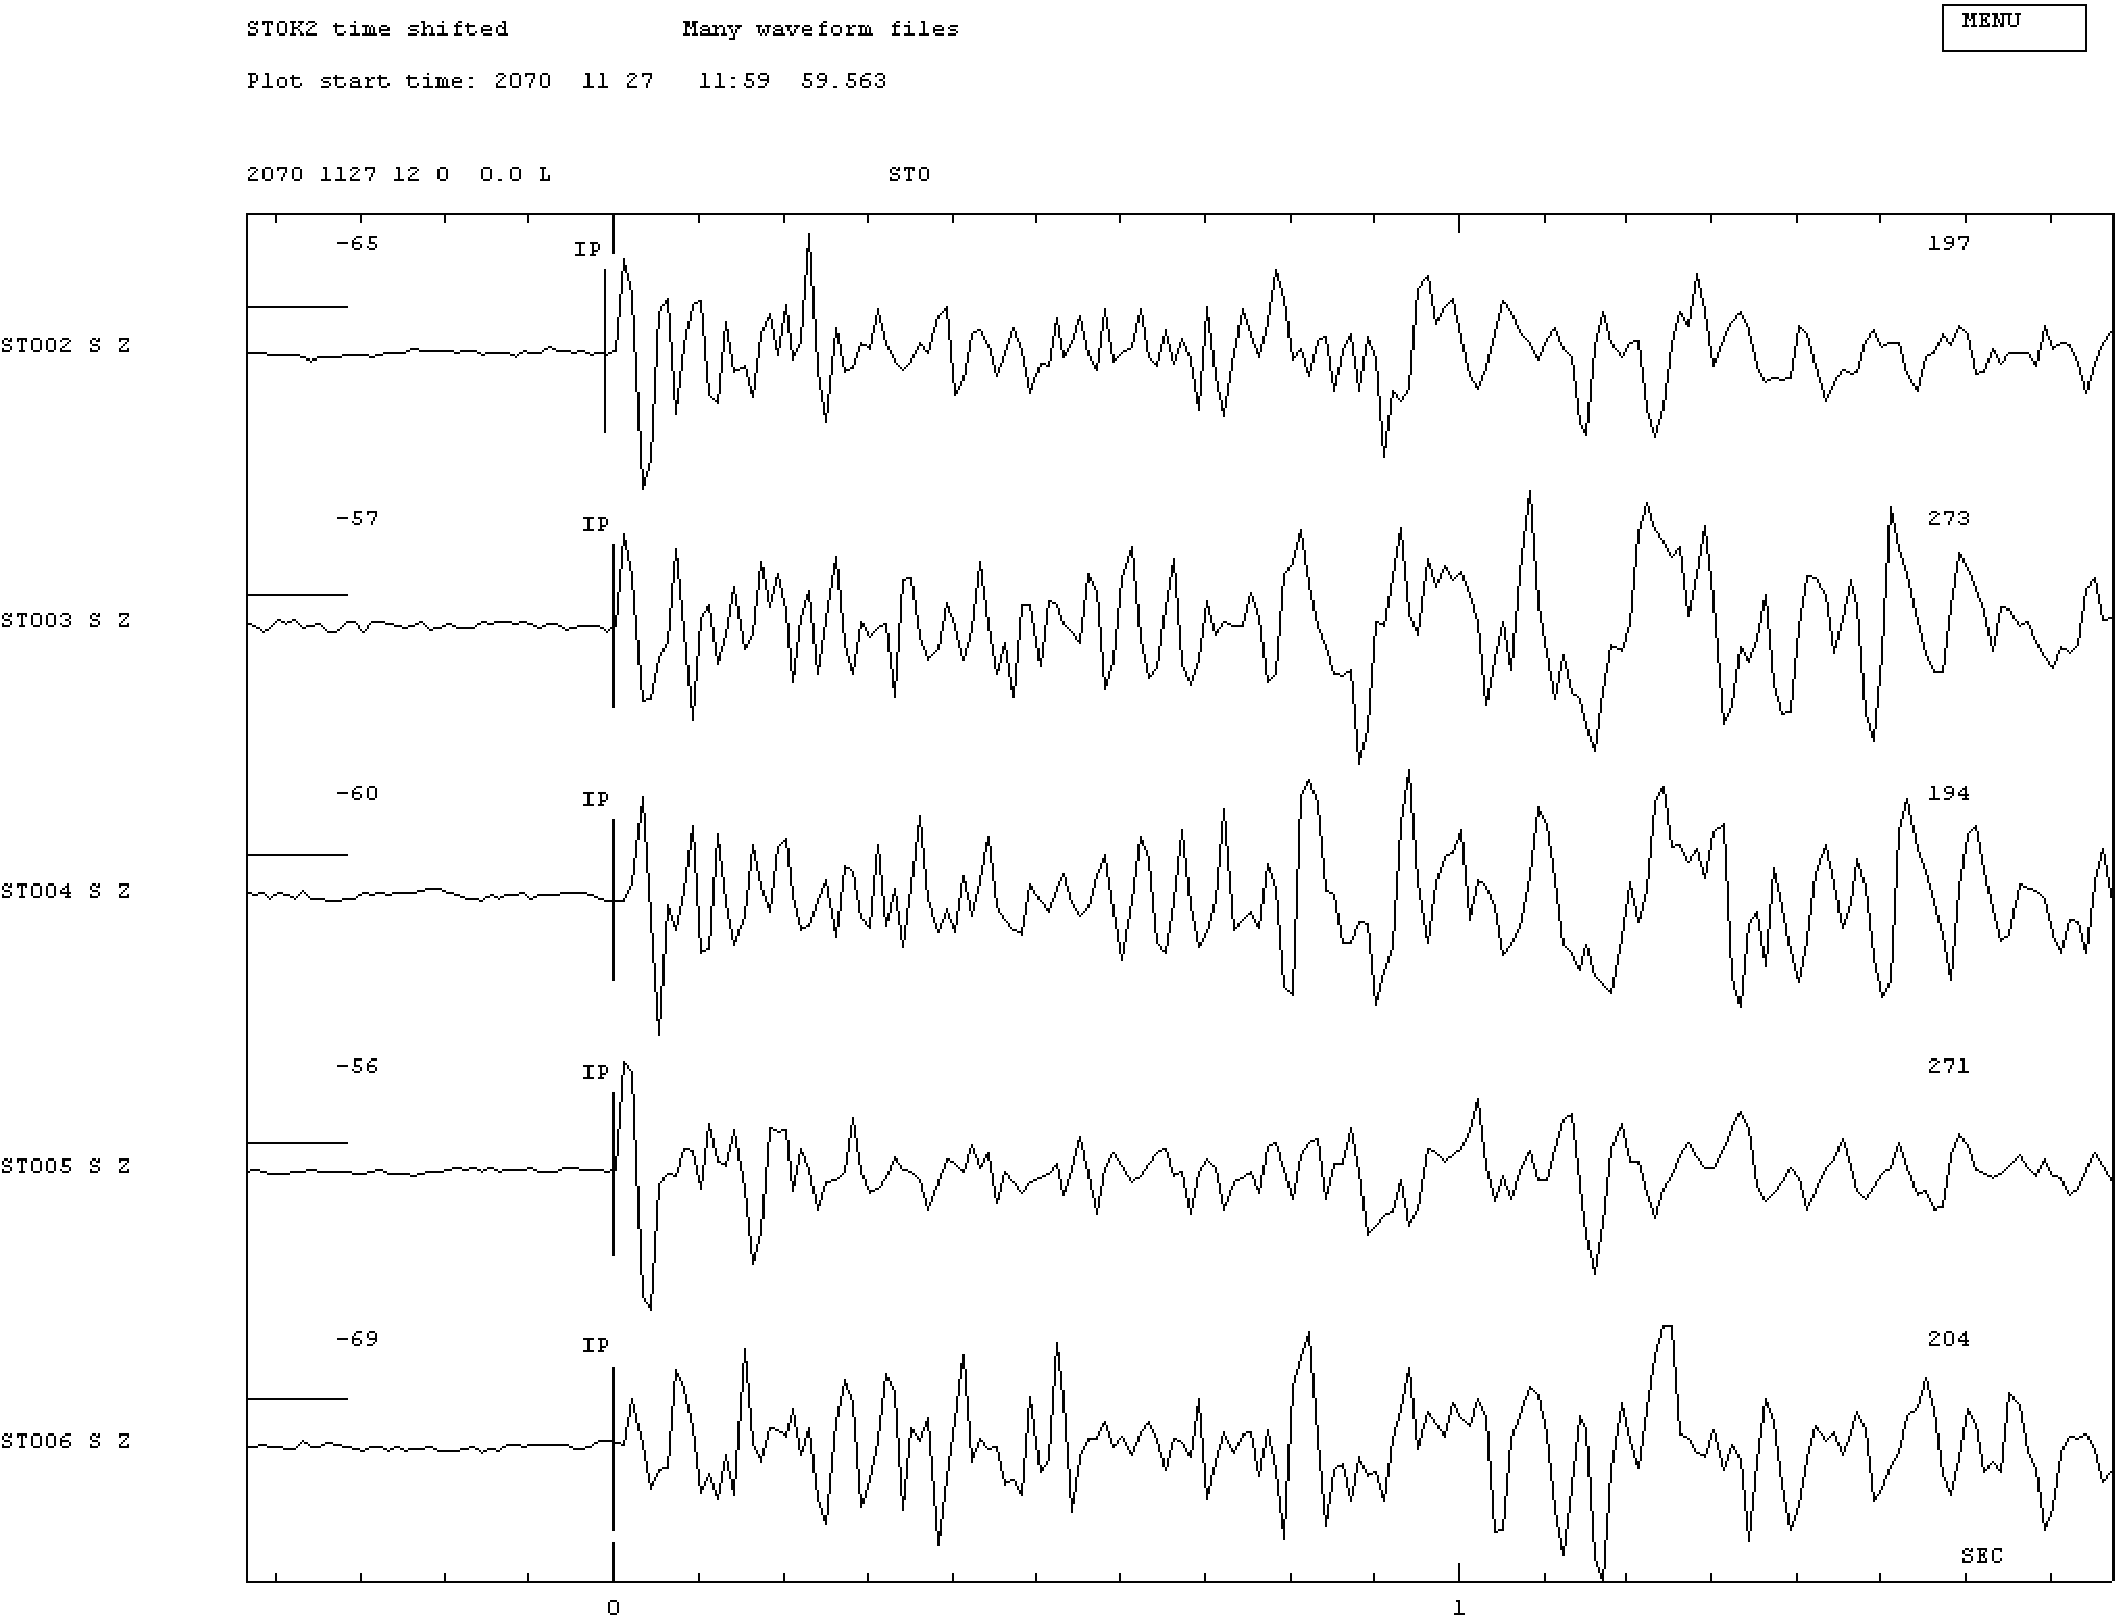
\includegraphics[width=0.9\linewidth]{fig/fig35}}
\caption{Example of aligning traces from 5 
events for the same station. Note that the alignment is critically 
dependent on the original P-picks.}
\label{fig:p_align}
\end{figure}

\textbf{WAVFIX, fixing time correction and channel names in SEISAN waveform file headers and make standard file names}

It can easily happen that a waveform file has a wrong time \index{Time correction}in the headers, or that individual channels have wrong timing, for example introduced by different delays in the acquisition system that are not accounted for. WAVFIX can change all \index{Header times}header times with a given constant \index{Time delay}time delay, or correct individual channels as specified in a parameter file (\texttt{wavfix.tim})\index{Wavfix.tim}. In addition, the file name will also be changed to reflect the header time change. \index{Waveform file name}Waveform file names were shorter in SEISAN version 6.0 so when using older files, the user might want to use standard file names. In cases where only channel names or timing of individual channels are changed, the filename can be kept the same. In this case a temporary file is created, which is later renamed to the original name. 

WAVFIX can also change polarity. This is done by setting the output channel and station codes to the same as the input values in \texttt{wavfix.def}. \index{Waveform file, fix headers}\index{Polarity change}\index{Polarity, correct}\index{Correctpolarity}

In case channel names are to be changed, this can also be done with WAVFIX. A definition file is needed for changing station, component or both. The parameter file name is \texttt{wavfix.def} and an example is given in DAT. For definition of the \texttt{wavfix.def}, see next section \ref{sect:file-conversion} on ``Conversion programs definition file''. 

WAVFIX can change header times and/or file names for one or many files. Before running the program, a list of file names must be made with DIRF. Below is an example where the header time is changed by 120 secs. No \texttt{wavfix.def} file is present (current or DAT directory).  

To correct the timing of individual channels, you need to create the file \texttt{wavfix.tim} in either the DAT or working directory. WAVFIX checks if the file is present and applies the correction from the file as default. The format of this file is as follows: 

Column 1-5: station code \newline
Column 7-10: component code \newline
Column 12-25: start date and time for time correction (can be empty) \newline
Column 27-39: end date and time for time correction (can be empty) \newline
Column 41:60: time correction to be added 

Example: 

\begin{verbatim}
 wavfix time correction applied to individual components
 stat  comp start time     end time       correction in
 a5    a4   yyyymmddhhmmss yyyymmddhhmmss seconds f20.3
 -----|----|--------------|--------------|--------------------
 TEST  SH Z 19500101120000 19600101120000 -0.015 
\end{verbatim}

File names of waveform files can be given to WAVFIX directly, from a \texttt{filenr.lis} file or from a Nordic format file. In case you choose the Nordic input, the waveform file names will be changed in the Nordic file (output file nordic.fix). This option is useful if you are correcting file names, since the entries in the S-files are otherwise not fixed. 

Example of running WAVFIX 

\verbatiminput{include/wavfix.run}

Note: WAVFIX ONLY works with SEISAN format 

\textbf{WAVFULLNAME}

Prints full filename including path\index{WAVFULLNAME} for a waveform 
file by searching directories and databases specified in 
\texttt{SEISAN.DEF}. Filename is to be given on prompt line, e.g. 
\texttt{wavfullname 1996-06-13-1248-15S.NSN\_\_003}. 


\section{File conversion and modification programs}
\label{sect:file-conversion}

\index{File conversion and modification programs}\index{Conversion programs} There are mainly two types of files to convert, parameter files with readings and related parameters and binary waveform files. 

\textbf{PARAMETER FILES}

\begin{tabular}{lp{10cm}}
CAT\_AGA: & Records the S-file header lines according to agency \\
EDRNOR: & Converts USGS monthly bulletins (EDR files) to Nordic format \\
GETpde: & Grap \index{GETPDE}PDE bulletin from USGS web page and add to SEISAN database\\
GIINOR: & Converts from Geophysical Institute of Israel\index{Israel} parameter format to Nordic \\
HARNOR: & Converts standard Harvard fault plane solutions to Nordic format \\
HINOR: & Converts Hypoinverse archive format to Nordic format \\
HYPNOR: & Converts from Hypo71 readings files to Nordic format files \\
HINNOR: & Similar to HYPNOR for Hypoinverse files \\
HSUMNOR: & Converts from Hypo71 summary file format to SEISAN format \\
ISCNOR: & Converts from ISC 96 column format to Nordic format \\
ISCSTA: & Converts ISC station list to SEISAN station list selecting specific stations. \\
ISFNOR: & Converts between ISF1.0 and Nordic \\
KINNOR: & Converts from Kinemetrics to NORDIC \\
NORGSE: & Converts between Nordic format and GSE parametric format \\
NORHIN: & Converts from Nordic format to Hypoinverse format \\
NORIMS: & Converts from  Nordic to and from IMS1.0 \\
NORHYP: & Converts from Nordic to HYPO71 format \\
PDENOR: & Converts a \index{PDE bulletin file}PDE bulletin file to NORDIC format \\
RSANOR: & Converts Andalucian Seismic Network data to NORDIC format\index{Andalucia} \\
SEIGMT: & Converts from NORDIC file to input for GMT \\
SELMAP: & Selects out a part of a MAP file \\
STASEI: & USGS station file or ISC station file to SEISAN \\
USGSNOR: & USGS/NEIC CDROM catalog conversion to NORDIC format\\
\end{tabular}
 

\textbf{CAT\_AGA, reordering of CAT file header lines}\newline
\index{CAT\_AGA}\index{Reorder Hypocenters}
When plotting hypocenters or doing seismic hazard work, it is the first header line in an S-file or CAT-file that is used since it is assumed that it is the prime estimate. When making compact files it is also the first header line, which is used. However, there can be a need for resorting the many type 1 
header lines for one or several events so that they are ordered according to \index{Agency}agency. It could e.g. be needed to put priority on all the ISC solutions, which then should be the first line in the file. \index{CAT\_AGA}CAT\_AGA will reorder the type 1 lines in a CAT file according to the order in which the agencies (3 character codes) are given by the user. If there are many agencies, they can be given in an input file named \index{Cat\_aga.par}\texttt{cat\_aga.par}, format is one agency per line in the first 3 columns. If the file is not present, the program will ask the user to enter the agencies manually. 
 The output file \texttt{cat\_aga.out} will contain the sorted events. 

\textbf{EDRNOR: USGS monthly bulletins (EDR files) to Nordic format}\newline
\index{EDRNOR}
Program to convert USGS weekly EDR files (ftp://hazards.cr.usgs.gov/weekly/mchedr*) to Nordic format. The program is written by \textbf{Mohammad Raeesi} (email Mohammad.Raeesi@student.uib.no). 

\textbf{GETPDE, USGS Preliminary bulletin to SEISAN}\newline
\label{page:getpde}
This Java program will get the PDE events from the USGS web page and store them
in a SEISAN database named PDE.\index{GETPDE} 
The program uses a parameter file getPDE.xml located in DAT with update peiod, data base to copy to etc. The program works under Window and Linux.
The program is written by \textbf{Ruben Soares Lu\'is} (ruben.so.luis@gmail.com). Contact the author for more information or consult our web pare for new documentation. 

\textbf{GIINOR, Geophysical Institute of Israel to SEISAN}\newline
The input files are the bulletin type files.\index{GIINOR}

\textbf{HARNOR, Harvard to Nordic }\newline
The standard moment tensor solutions given by Harvard (\url{http://www.globalcmt.org/CMTsearch.html}) are converted to Nordic format. Strike, dip,  rake  and moment tensor solution is written out.\index{HARNOR}\index{Harvard moment tensor solution }

\textbf{HINOR, Hypoinvers archive format to Nordic}\newline
The input files are the archive type. All events are assumed local.
No check if header time corresponds to phase times. \index{HINOR}

\textbf{HYPNOR, converting \index{HYPO71 files to Nordic files}HYPO71 files to Nordic files}
\newline
\index{HYPNOR}
Input is just filename of HYPO71 file. A similar program for HYPOINVERSE files is HINNOR. 

\textbf{HINNOR, converts from Hypoinverse to NORDIC format} \newline
\index{Hypoinverse to Nordic}\index{HINNOR} This program works like HYPNOR. 

\textbf{HSUMNOR, HYPO71 summary file format to NORDIC format } \newline
Note that the program only converts to header lines. 

\textbf{ISCNOR, converting ISC bulletin file to Nordic format } \newline
This program works with the ISC fixed 96-column format as e.g. distributed on CDROM (files of type FFB). The program \index{ISCNOR}can select out subsets of ISC data using a latitude-longitude window, depth and prime magnitude. Any of the magnitudes Ms and mb are used. Before 1978, there was only mb on the CD's. More detailed selection can be done on the output file later with SELECT. Since the amount of data is very large it is also possible to write out only the hypocenters. Note that ISC now writes in ISF format also, which can be converted with ISFNOR. 

Newer CD's have compressed data and cannot be used directly. files must be copied to disk first, decompressed and then handled as single files. \index{ISC to Nordic}\index{ISC} 

The program will first check if a file with agency codes called agency.isc is present. If so the station codes are read from this file (same format as files on CDROM). The program will also check the beginning of the data input file for a possible list of agencies and station coordinates. If present, the stations coordinates are read and converted to SEISAN format and additional codes read in. The agency codes are needed in order to identify in plain text the various agencies used. 

Principles in conversion: 

\begin{tabular}{lp{10cm}}
Phases: & The phases out can be either the phase ID's sent to ISC or the ISC reinterpreted phases 
(given with a number code in the input file). If the user supplied phases are used, 
parenthesizes are removed, and if P/PKP etc is given, it is replaced by P. \\
Times: & If day is incremented relative to origin time day, it is carried into the hours, which can be 
more than 24. \\
Agency: & It is assumed that it is the same agency for hypocenter and first magnitude. Magnitude is    
checked for agency, if blank, it is assumed also to be the same as for hypocenter. Only first 
3 characters of code is used. \\
Stations: & Only first 4 characters of code are used. \index{Station, only 4 characters} \\
Depth: & If no error on depth, a depth fix flag is set. \\
First motion: & Only C or D are used, ISC codes J and B are ignored. \\
Hypocenter orders: & ISC put the best solution last, here the order is reversed, and the prime estimate 
is  first. \\
Duration magnitude: & Change D to C for type. \\
Distance indicator: & If station furthest away is less than 1000 km indicator is L, between 1000 and 
3000 km indicator is R and if more than 3000 km indicator is D. 
If no stations are present  the type is set to D. 
\end{tabular}

In order to relocate an event and compare to ISC location, the ISC reidentified phases must be used (option 2, see below). This has the disadvantage that phases not used by ISC (mainly S-phases of local earthquakes) are weighted out in the output file. If option 3 is used, the ISC identified phases are selected if there and if no ISC identification is given, the local reported phase is used. The output file for option 2 and 3 looks the same except that for option 2, the user-defined phases are weighted out. The residuals given in the output file are always relative to the ISC identified phases. 

Running ISCNOR: 

Below is an example of a run where a latitude - longitude window has been used.  

\verbatiminput{include/iscnor.run}

The file input can be from a CDROM as in the example above. In that case, the whole CDROM can be read or a smaller time interval can be given. The input can also be from a single file and the program will then ask for the next file when the first has been converted. If many files are to be converted, a list of file names can be made with DIRF and \texttt{filenr.lis} entered as an input file name. The Nordic format output file is \texttt{iscnor.out} and the station list is in \texttt{isc.sta} which has the format used by SEISAN. Optionally, output can also be in the original isc format, however that requires setting a flag in the program and recompiling, see program source code. 

\textbf{ISCSTA, selecting stations in the complete ISC station file} \newline
\index{ISCSTA}
The complete station list in the ISC list is very large and it is often an advantage to use a smaller subset, although HYP can use the whole list. The program can select out subsets of stations in both SEISAN and an older ISC format.\index{ISC} The program will read an S-file, find how many different st\index{Station coordinates}ations there are and select those stations out of a station file, which can either be in SEISAN (=HYPO71) format or ISC format (automatically determined). The output is in SEISAN format. If no S-file is given the input station file is assumed to be in ISC format and the whole file will be converted to SEISAN format.\index{Station selection} 

\textbf{KINNOR, Kinemetrics to NORDIC} \newline
Converts .PCK file output of EDPPICK to file in SEISAN format. Many events are converted from one file. The program is based on program from Kinemetrics by \textbf{Christopher S. Lim}. For info on how conversion is made, see program source code. \index{Kinemetrics}\index{PCK files}\index{EDBPICK picking program} 

\textbf{ISFNOR, ISF1.0 to and from Nordic}\newline
\index{ISFNOR}
The ISF format is used by the ISC\index{ISC} and is an extension to the IMS format. The program is based on the routines provided by the ISC for reading and writing ISF, and the SEISAN standard routines for reading and writing Nordic data. The program converts in both directions. All possible information is converted. Information on the ISF format can be found on the ISC website (\url{http://www.isc.ac.uk}). It is recommended to use ISF format for data exchange with ISC. 

\textbf{NORIMS, IMS1.0 to NORDIC format}.\newline
\index{NORIMS} \index{NDC}
The IMS1.0 (International Monitoring System) is a new version of the GSE format and very similar. The program can partly be used for the new ISF (IASPEI Seismic Format) which will include all of the IMS format an additional information needed by ISC and NEIC.\index{IMS1.0}\index{International Monitoring System}\index{ISF format}\index{IASPEI Seismic Format} The program and the following description is by \textbf{Mario Villagr\'an}. The program works with the IMS1.0:SHORT format (phase-readings/origin files) and the program works both ways. 

\indent IMS1.0:SHORT $\Rightarrow$ Nordic\newline
\indent Nordic $\Rightarrow$ IMS1.0:SHORT 

The IMS1.0:SHORT format is exactly the one used at the IDC International Data Center (Vienna, Austria). In addition some features used by the ISC International Data Center and the Spanish NDC National Data Center had been added. Magnitudes in IMS format use many characters, the Nordic format allows only one; the following rule is followed: 

IMS \verb|     | Nordic\newline
For mb $\rightarrow$ 'b' \newline
For MS $\rightarrow$ 'S' \newline
For ML $\rightarrow$ 'L' \newline
For MD $\rightarrow$ 'D' \newline
For Ml $\rightarrow$ 'l' \newline
For MN $\rightarrow$ 'N' \newline
For mblg$\rightarrow$ 'G' \newline
For ms $\rightarrow$ 'S' \newline
For MB $\rightarrow$ 'B' 

%\textcolor{red}{pv-change: is conversion of mB and mS correct?}

%\textcolor{red}{pv-change: 
IMSNOR do not include code magnitude.

The maximum likelihood magnitudes mb1, mb1mx, ms1, ms1mx, etc are 
pending. IDC still does not have documentation and they may be changed. \newline
Single measurements of magnitude/station are parsed as comment lines 
(type 3) starting with symbol ``\$''. When importing data from IMS 
format, only the ``Event IDC'' number is parsed and included into a comment 
line (type 3) of Nordic, together with the ellipse dimensions orientation 
and the mb standard deviation. \newline
All parameter values read that exceed 
field limits of Nordic (Amplitude, velocity, snr, etc) have been set 
to the maximum or minimum possible, example: if snr $>$ 999.9 then snr=999. 
For conversion from Nordic to IMS it is necessary to use both the 
\texttt{hyp.out} and \texttt{print.out} files; The reason is that IMS includes 
many parameters that need to be searched in both files. \newline
When converting 
to IMS format, the user can specify the start numbering for the first event and phase 
in the file; ignoring will assume (1,1). It is optionally also possible 
to set the no location flag in the 
output header lines. 

\textbf{NORGSE, NORDIC from and to GSE parametric format} \newline
\index{NORGSE}
The program (written by \textbf{Mario Villagr\'an}) converts parametric data 
between Nordic and GSE2 format. It ca\index{Nordic to HYPO71}n be 
used interactively or by giving the options as arguments. Type 
\texttt{norgse -help} to see the options.\index{GSE format}

\textbf{NORHIN, From Nordic to Hypoinverse format} \newline
\index{NORHIN}\index{Hypoinverse format}
The program is started by typing \texttt{norhin input-file}. The output file is norhin.out. 

\textbf{NORHYP, From Nordic to HYPO71 format (SUN and PC)} \newline
\index{NORHYP}
The program is written by \textbf{F. Courboulex}. The program asks for the 
input file name and the output file name is \texttt{norhyp.out}. 

\textbf{PDENOR, converting PDE bulletin file to NORDIC format} \newline
\index{PDE}\index{PDENOR}PDE distributes bulletins on e-mail, both a monthly bulletin and a weekly bulletin (different formats). The program converts one of these files to Nordic format and put the file into a standard SEISAN database called PDE for the monthly files and PDEWE for the weekly files. This database must have been created before running the program. Both CAT and S-files are made and SELECT and EEV can be used afterwards \index{PDE e-mail} 

\textbf{RSANOR} \newline
Program converts between format used by ``Red Sismologica de Andalucia'' and 
a few others in Spain. \index{Spain}

\textbf{SEIGMT, Nordic to GMT input} \newline
The program SEIGMT\index{SEIGMT} reads information from Nordic or compact files and writes the parametric data to files that can be used as input for GMT\index{GMT}\index{Generic Mapping Tools}(Generic Mapping Tools, \url{http://gmt.soest.hawaii.edu/}). The user can choose a scaling for the magnitudes and also select a magnitude type order. The scaling option is useful if you wish to scale the symbol size of your epicenters with magnitude. The magnitude type order defines, which magnitude should be taken in case several magnitudes have been determined for one event. If you don't give a magnitude order, the program chooses the largest magnitude. 

The files written by SEIGMT are: 

\texttt{gmtxy.out} - event locations, to be plotted with psxy \newline
\texttt{gmtxyz.out} - event locations and depths, to be plotted with psxy \newline
\texttt{gmtstxy.out} - station coordinates (longitude, latitude and station code) \newline
\texttt{gmtpath.out} - travel path data, to be plotted with psxy \newline
\texttt{psmeca.out} - fault plane solutions, to be plotted with psmeca (Aki and Richards convention) 

\textbf{SELMAP, selecting a subsection of a MAP file} \newline
\index{SELMAP}
The program can retrieve parts of a large MAP file written in SEISAN map format. On the SEISAN web site or on the SEISAN CDROM, very detailed global mapfiles are available in SEISAN format. The file originally comes from the USGS\index{USGS}. SELMAP can select out part of a MAP file in a latitude-longitude grid. The MAP files consist of several small segments and a segment is selected if at least one point is inside the specified grid. \index{Map files}

\textbf{STASEI} \newline
\index{STASEI} 
Converts the official global station file from USGS (comma format) or ISC global station file to SEISAN station format (same as HYPO71 format with SEISAN extension for 5 letter station codes). A list of most global stations are now found on the SEISAN CD. It seesm that the USGS format is no longer used. \index{Station coordinates}\index{Global station coordinates}

\textbf{USGSNOR, USGS catalog to NORDIC format} \newline
\index{USGSNOR}
The program converts USGS CDROM hypocenters to NORDIC format. Most of the information is used. If more than 3 magnitudes are available, only the 3 first are used. The number of stations is 
included when available. The depth is indicated as fixed in all cases where the operator has been used (A,N,G). Macroseismic information is included with max intensity. The residual standard deviation is put into rms column. Event types are set to R. Magnitude types are converted as follows: 

UK is made blank \newline
b is replaced by B \newline
s is replaced by S \newline
D is replaced by C \newline
w is replaced by W 

\textbf{WAVEFORM CONVERSION PROGRAMS}

This group of programs are mostly converting waveform files from some format to SEISAN although a few also convert from SEISAN to some other, mostly standard, formats. Most programs convert from binary to binary formats. \newline
Many instruments come with conversion programs to some standard format like PCSUDS or MINISEED, and these have often been used to convert to SEISAN instead of writing programs reading the original files directly. Many such conversion programs work on PC so the corresponding SEISAN programs only work on PC. However, since the PC files can be read directly on Sun, this should not present a problem. Many programs have VERY LITTLE documentation, look in source codes for more information. 

The number of programs are forever increasing with new recorders coming onto the market and new formats coming in use and others going out of use and it is becoming increasingly difficult to keep track of it all. For this release of SEISAN it has not been possible to test all programs on all platforms. An attempt has been made to standardize the programs. A general problem is that many seismic recorders and formats do not provide proper identification of the channels. In the worst cases, there are no station codes, only channel numbers and in very many cases, there is no room for proper component information. This is being taken care of by having a definition file, and only one format for the definition file is used, see below. This is also used with program WAVFIX. \newline
Most programs work in the standard way with a \texttt{filenr.lis} file as input (made with DIRF). \newline
The response information is seldom in the original files and in most conversion programs, the response information is taken from the CAL directory. If no response information is available, a message will be given. For each program, a comment will be given as to the status of testing and on which platforms they operate. If the channel definition file option is implemented, the array dimensions will be SEISAN standard. \newline
The program SEIPITSA might be an easy way to convert between 1-column ASCII data and SEISAN (see below)\index{ASCII waveform format}. 

When converting between the major analysis format (MiniSEED, SEISAN, SAC and GSE) mostly using program WAVETOOL, only SEISAN and MiniSEED will preserve the network and location codes as well as the flag for uncertain timing since the other formats only partly have room for this information. \index{Uncertain timing flag}\index{Location code}\index{Network code} 

\textbf{Conversion programs definition file}
\index{Conversion of station codes}\index{Conversion of component codes}\index{Waveform conversion programs}

The conversion programs use a common format for the definition file for naming station and channels. The definition file is named programname.def as e.g. sudsei.def. The definition file can be in the working directory or the DAT directory. The conversion program will first look in the working directory for the file and then in DAT. The conversion of codes can take place in 2 ways (see below for details): 
(1) An input station and component code is converted to an output station code and component, (2) an input channel number is assigned a station and component code. The advantage of (1) is that the conversion is independent of the channel number or order, however, the user must then know the default station and component names generated by the conversion program. 

Default assignment of station code and component: \newline
This is very much dependent on the conversion program used since some data files have complete 

information and others very little, see description of individual programs in manual or at start of source codes. In all cases, the conversion program will make both station and component codes based on what is available of information in the input files. IT IS THESE CODES THAT are used for input code as described below. In order to find out what they are, it is easiest to run the conversion program once (without a def file) and see what codes the program assign. Alternatively, some of the programs have documentation in the manual. Some of the station codes might be instrument serial numbers, which are not always known. Therefore, running a test might be the best way to find out. \index{Serial number, instrument}\index{Network code, put in waveform file}\newline
In addition to converting channel codes, the def file can also give SEISAN waveform file header information and network code as it appears in the file name. If no network code is given, the network code will be the station code of the first channel. 

Principle of conversion in order of precedence: 
\begin{enumerate}
\item
 Both station and component given on input: Converted to what is given for output station and component. 
\item
 If both are not present, the channel number is used. 
\end{enumerate}

\begin{verbatim}
Header line text (29 char)... NetCd (5 chars), Comment for next line
Header for REFTEK             NEWNT 
chan stati  comi stato  como, In and output definitions, comment for next line
   1 BO11   S  Z BOM    B  Z  
     BO12   S  N BOM    B  N  
     BO13   S  E BOM    B  E  
\end{verbatim}

The first line is just a comment line, must be there in any format. Here it shows where the network code is positioned as indicated by NetCd. 

The second line gives the header information for the SEISAN main header, which are the first 29 characters. The file name network code is also given and is here NEWNT. Format a29,1x,a5. 

The third line is just comment to indicate the position of the columns in the following lines (max 200). A line must be there. The abbreviations are: 

\begin{tabular}{lp{10cm}}
chan: & Channel number, optional unless no input station and component given. \\
stati: & Input station code, 1-5 chars \\
comi: & Input component code, 4 characters \\
stato: & Output station code, 1-5 characters \\
como: & Outut component code, 4 characters. First character MUST be S, L, B, A, or I,             last character MUST be Z, N or E, all upper case. \\
\end{tabular}

Format i5,1x,a5,2x,a4,1x,a5,2x,a4 

The conversion programs are listed below

\begin{tabular}{lp{10cm}}
AHSEI:  & AH ASCII to Seisan, little tested\\
ARCSEI: & Reftek archive to Seisan, windows only \\ %\textcolor{red}{pv-change: windows only} \\
ASCSEI: & ASCII to SEISAN \\
BGISEI: & Beijing Geodevice Institue to SEISAN \\
CITSEI: & CityShark to SEISAN \\
CNVSSA: & Kinemetrics SSA to Kinemetrics Dataseis \\
CNVSSR: & Kinemetrics SSR to Kinemetrics Dataseis \\
DIMASSEI: & USGS Dimas to Seisan\\
DRSEI: & Sprengnether recorders to SEISAN \\
GIISEI: & Geophysical Institute of Israel to SEISAN \\
GSRSEI: & GeoSig to SEISAN \\
GSESEI: & See WAVETOOL \\
GSERESP: & Conversion between GSE and SEISAN response files \\
GURSEI: & G\"uralp to SEISAN \\
IRISEI: & From IRIS ASCII to SEISAN  \\
ISMSEI: & ISMES to SEISAN \\
KACSEI: & Kinemetrics ASCII acceleration to SEISAN \\
KINSEI: & Kinemetrics Dataseis to SEISAN \\
K2SEI: & Kinemetrics K2 to SEISAN \\
LEESEI: & Willy Lee system to SEISAN \\
LENPCQ: & Converts from Lennartz to PCEQ to PCEQ format \\
LENSEI: & Lennarts ASCII to SEISAN \\
M88SEI: & Lennartz MARS88 to SEISAN \\
MSFIX: & Rewrite MiniSEED files \\
NANSEI: & Converts from Nanometrics to SEISAN  \\
NEISEI: & Converts from NEIC CDROM waveform data to SEISAN \\
NRWSEI: & Geol. Survey. of Northrhine-Westphalia format to SEISAN format\index{NRWSEI}\index{Norhtrhine-Westphalia} \\
OS9SEI: & Converts SEISLOG files to SEISAN waveform files \\
PITSA: & Conversion programs described with program PITSA \\
PCQSEI: & Converts from PCEQ to SEISAN  \\
PDASEI: & Geotech Instruments PDAS to SEISAN  \\
PSNSEI: & Public Seismic Networks to SEISAN \\
QNXSEI: & SEISLOG QNX to SEISAN \\
RDSEED: & IRIS program to read SEED volumes \\
RSASEI: & Conversion from Andalucian Seismic network to SEISAN\index{Andalucia} \\
RT\_SEIS: & Reftek Passcal format to SEISAN conversion \\
SEI2PSXY: & Convert waveform data to trace input for psxy \\
SEIM88A: & Conversion from SEISAN to MARS88 ASCII format \\
SEISAN2MSEED: & From SEISAN to MiniSEED \\
SEISAF: & SEISAN to SESAME ASCII \\
SEIPITSA: & SEISAN $\Leftrightarrow$ PITSA ASCII \\
SGRSEI: & SeisGram to SEISAN \\
SISSEI: & Sismalp format to SEISAN format \\
SILSEI: & SIL network ASCII files to SEISAN \\
SUDSEI: & PCSUDS to SEISAN \\
TERSEI: & Terra ASCII to SEISAN \\
WGSSEI: & WGSN format to SEISAN 
\end{tabular}

For each program, a summary of capabilities is mentioned: The platforms 
available (all for all or specific name), channel definition file 
available (chan. def. yes or no) and if the program will look for 
response files in the CAL directory to insert in the headers (resp. yes or no). \newline
If you do not find the conversion program here, look on the  ORFEUS 
website \index{ORFEUS}for other programs that might convert to one 
of the formats used above. \newline
(\url{http://orfeus.knmi.nl/other.services/conversion.shtml}). 

%\textcolor{red}{lo-change}
{
\textbf{AHSEI, AH ASCII to SEISAN} \verb|                  | all, chan. def. yes, resp yes\newline
\index{AHSEI}
Converts AH ASCII files to Seisan format.
}

\textbf{ARCSEI, Reftek archive to SEISAN} (windows only) \newline 
% \textcolor{red}{pv-change: windows only}\newline
\index{ARCSEI}
ARCSEI is a program to automate the extraction of data from a RefTek data archive and the conversion to SEISAN format. \index{REFTEK}The program works interactively and with a simple text interface that asks the user to enter the details for the data extract. Based on the user selected criteria the program (1) extracts the data from the archive in Passcal format using ARCFETCH, (2) \index{ARCFETCH}converts the Passcal data files to SEISAN format using RT\_SEIS, \index{RT\_SEIS}and (3) merges the SEISAN files if merging is activated by the user, using SEISEI. The program is written in Fortran and works on Windows only. 

The ARCSEI program can be used in various ways: 

\begin{itemize}
\item
to extract a single time window from one or several stations 
\item
to extract several time windows from one or several stations 
\item
to extract sequential time windows from one or several stations 
\end{itemize}

The ARCFETCH and RT\_SEIS programs, both part of the RefTek software package, have to be installed (see RefTek documentation) and the PATH variable set to include the directory where the programs are stored. It is assumed that the RefTek data archive exists and that the user is familiar with the content of the archive. The archive content can be shown with the command ARCINFO. To test that the program is installed correctly, open the Windows command tool (from the menu, or by selecting Start . Run . cmd) and type ARCSEI $<$RETURN$>$. 

The definition file: \texttt{arcsei.def}

The purpose of the definition file is to set some parameters needed to run ARCSEI, however, the program also works without. The arcsei.def file can either be stored in the seismo/DAT directory, or the current working directory. The program first checks in the current directory. The arcsei.def file should be adjusted to the user's set-up, before ARCSEI is started. \index{Arcsei.def} 

The parameters are: 

\begin{tabular}{lp{10cm}}
ARCHIVE: & The path of the RefTek data archive, can also be entered manually at run time. \\
OUTPATH: & The directory in which the SEISAN files are to be stored. The default is `.\textbackslash'  
(the current directory). \\
MERGE: & Select if SEISAN files from several stations for the same time interval should  
be merged (Y), or not (N). \\
NETWORK\_CODE: & Network code used in case SEISAN files are merged. \\
CHANNEL: & Data channel in RefTek archive consisting of the unit, stream and channel  
(unit,stream,channel). The * can be used as wildcard to select all streams or  channels, BUT not to select all units (since ARCFETCH is used in cooked mode,  which means that the time interval extracted  matches the input start- and end-time. \\
\end{tabular}

Example of the \texttt{arcsei.def} file 

\verbatiminput{include/arcsei.def}

How to run the program: 

ARCSEI is started from the Windows Command Tool (cmd) by typing  

\verbatiminput{include/arcsei.run}

Type channel and $<$RETURN$>$, if defined in arcsei.def channels are listed, otherwise an example is shown. The channel is given as unit,stream,channel. Wildcards can be used for stream and channel, but not for the unit. 
\begin{verbatim}
NEXT CHANNEL OR RETURN TO CONTINUE 
\end{verbatim}

Additional channels can be entered, to continue press $<$RETURN$>$. 

\begin{verbatim}
ENTER START-TIME (YEAR:DAY-OF-YEAR:HOUR:MINUTE:SECOND)
          EXAMPLES: 2000:200:12 
                    2000:200:12:15 
                    2000:200:12:33:15 
\end{verbatim}

Type start time as year:day-of-year:hour:minute:second. Minute and second can be omitted.  

\begin{verbatim}
NEXT START-TIME OR RETURN TO CONTINUE 
\end{verbatim}

Additional start times can be entered, to continue press $<$RETURN$>$. 

\begin{verbatim}
ENTER END TIME USING ONE OF 3 OPTIONS: 
- ABSOLUTE TIME AS YYYY:DDD:HH:MM:SS (LIKE START-TIME)
- +SECONDS FOR TIME INTERVAL (e.g. +300)
- ++SECONDS FOR MULTIPLE INTERVALS(CONTINUOUS EXTRACT, e.g. ++300) 
\end{verbatim}

Specify the end time, either in the same style as for the start time (only if one start time), or in some cases more useful, the desired time window in seconds, by entering +seconds. If sequential time windows are to be extracted, use ++ seconds. The user is then asked how many time windows should be extracted. It is thus possible e.g. to extract 10 consecutive windows of 600 seconds. 
Only if sequential extract windows specified: 

\begin{verbatim}
ENTER NUMBER OF CONTINUOUS WINDOWS 
\end{verbatim}

After the program has finished, the data in SEISAN format can be 
found in either the current directory (default) or in the OUTPATH 
directory if the variable is specified in \texttt{arcsei.def}. The temporarily 
created files are deleted automatically. 

\textit{How it works}

ARCSEI reads the user input that specifies what should be extracted from the RefTek archive and then calls the programs ARCFETCH, RT\_SEIS and SEISEI. For temporary data storage ARCSEI creates the directory arcsei\_temp under the current directory. The arcsei\_temp directory is automatically deleted upon program completion. 

\begin{enumerate}
\item Create empty arcsei\_temp directory 
\item Arcfetch 

The arcfetch program performs the data extraction from the RefTek 
archive. A complete list of the command line input of arcfetch can 
be obtained by starting the program without additional options. 
ARCSEI starts arcfetch in the following way: 

arcfetch archive channel,start-time,end-time -o OUTPATH -c 

Where:  

-o OUTPATH:  Specifies the output path for arcfetch, always arcsei\_temp   \newline
-c:  Specifies cooked mode, which means that the time interval extracted   
matches the input start- and end-time (this is not the case, when not running in  
cooked mode)  

Example:  \newline
\texttt{arcfetch G:\\ARCHIVE 8020,1,*,2000:200:12,+10 -oarcsei\_temp -c}
\item rt\_seis 

RT\_SEIS converts all files with the suffix `rt' in arcsei\_temp to SEISAN format. RT\_SEIS reads the \texttt{RTU.INI} file for station definition, if the environmental variable RTU is set to point to the \texttt{RTU.INI} file (see RT\_SEIS section below). 
\item SEISEI 

SEISEI, if merge is selected, merges all SEISAN files in the arcsei\_temp directory. 

\item move 

Finally all files (single or merged) are moved to the OUTPATH directory or the current directory if OUTPATH is not defined. In case multiple stations are selected, ARCSEI runs steps (1) and (2) in a loop, before the data is merged and moved. In case several time windows are selected, ARCSEI runs steps (1) to (4) in a loop, and in addition a second loop over multiple station (1) and (2). If sequential time windows are specified, ARCSEI computes multiple start times and works as if these time windows were user specified. All, def. File yes, resp yes 
\end{enumerate}

\textbf{ASCSEI, ASCII to SEISAN} \verb|                  | all, chan. def. yes, resp yes\newline
\index{ASCSEI}\index{ASCII, convert to SEISAN}
Converts a single column file to a one channel SEISAN file. Date, time, sample rate, station and component must be entered manually. The user is ask for a scale factor, normally it is 1.0. If input numbers are smaller than 1.0, a scale factor must be used since numbers are written out as integers. The input file must contain only a column of numbers adn no headers. 

\textbf{BGISEI, Beijing GEODEVICE FORMAT (BGI) to SEISAN.}
\verb|| Linux, PC, chan. def. yes, resp yes\newline
\index{BGISEI}\index{China}
The program to convert waveform files from BGI to SEISAN format is called BGISEI. The instrument response in the original files is not used. The program has only been tested with data recorded in Cuba. The program is written by \textbf{Bladimir Moreno}. 

\textbf{CITSEI, CityShark to SEISAN} \verb|              | all, chan. def. yes, resp yes \newline
Converts from CityShark ASCII to SEISAN. \index{CityShark}\index{CITSEI}Components S Z, S N, S E are assumed for the 3 channels. Assume 3 channels files only, all channels same sample rate and number of samples. 

\textbf{CNVSSA and CNVSSR Kinemetrics accelerometers to Kinemetrics Dataseis} \verb|       | PC \newline
The programs are supplied by Kinemetrics to convert from SSA and SSR formats to Kinemetrics Dataseis. To further convert to SEISAN, use program KINSEI. Only PC executable programs are available. The data is 16 bit.\index{SSA, Kinemtrics}\index{SSR, Kinemetrics} 

\textbf{CSS} \newline
At the moment there is no direct conversion from CSS to SEISAN. It is possible to convert CSS data to SAC or GSE using other tools like codeco, Geotool and SAC, and then convert to SEISAN format. \index{CSS format} 

%\textcolor{red}{lo-change}
{
\textbf{DIMASSEI, USGS DIMAS to SEISAN} \verb|                  | all, chan. def. yes, resp yes\newline
\index{AHSEI}
Converts Dimas files to Seisan format.
}

\textbf{DRSEI, Sprengnether data recorders to SEISAN} \verb|   | 
all, chan. def. yes, resp yes \newline
\index{DRSEI}\index{Sprengnether}\index{DR3024 and DR3016}
Converts Sprengnether DR3024 and DR3016 to SEISAN format. These two formats are slightly different, but the program makes the adjustment. Only essential information is read in and only 4 lowest digits of serial number are used. If station codes are set up, these are used, else the serial numbers are used for station codes. 

\textbf{GIISEI, Geophysical Institute of Israel to SEISAN}
\verb|  | all, chan. def. yes, resp yes\newline
\index{GIISEI}
Converts Geop\index{Israel}hysical Institute of Israel imported DAQ files to SEISAN format. The initial station codes are as defined in file, can be converted with the normal .def file. If 4.th character of station name indicates component (N or E), that is blanked out and transferred to 4.th character of component name BEFORE using the def file conversions. 

\textbf{GURSEI, G\"uralp to SEISAN} \verb|   | all, chan. def. yes, resp yes\newline
Converts G\"uralp GCF files to SEISAN format, only works with one channel data. Maximum number of samples as defined in seisan, at least 1 200 000, channels codes can be defined using the gursei.def 
definition file. If no definition file, the station name is the first 4 letters from internal station name and the component is B Z. \index{G\"uralp}\index{GURSEI}\index{GCF format}

\textbf{GSERESP, conversion between GSE and SEISAN response files} \verb|     | all \newline
The program provides conversion between SEISAN, GSE1 and \index{GSERESP}\index{Response, GSE}GSE2 response files. The response can be given in frequency, amplitude and phase (FAP) triplets or in poles and zeros (PAZ). Since the number of values in the GSE format is unlimited the conversion from SEISAN to GSE only changes the format, whereas converting from GSE to SEISAN, if the number of FAP triplets is more than 30 or the number of poles and zeros larger than 37, the response in SEISAN format will be approximated by 30 FAP triplets. The output files in SEISAN format will have the default S\index{GBV recorder}EISAN response filenames (see RESP program and SEISAN response format). Output files in GSE format will include the station name, the component, number 1 or 2 for GSE1 and GSE2 respectively and end on `.CAL' (e.g. MOR\_SHZ2.CAL (GSE2), KONO\_BZ\_1.CAL (GSE1). 

\textbf{GSRSEI, GeoSig to SEISAN} \verb|     | all, chan. def. yes, resp yes\newline
\index{GSRSEI}\index{GeoSig}\index{GeoSys}
Converts from GBV recorders to SEISAN. GeoSig was earlier GeoSys. Before version 8.1, there was a bug in program so start time was wrong by the amount of the prevent time. 

\textbf{IRISEI, IRIS ASCII to SEISAN} \verb|     | all, chan. def. no, resp yes \newline
\index{IRISEI}\index{GSN}\index{Quanterra}
The input format is the variable ASCII download format used on the GSN Quanterra stations. The format is used in connection with SEISNET. The program only works if input file has more than 1000 samples. \index{IRIS}ISMSEI, ISMES to SEISAN PC, chan. def. no, resp no ISMES is an Italian seismic recorder. This is the first version of the program made by IIEES in Iran. The program can convert\index{ISMSEI} one file with up to 3 channels. \index{IRIS}

\textbf{KACSEI: Kinemetrics ASCII acceleration to SEISAN} \verb|   | all, chan. def. yes, resp yes 
\newline
\index{Kinemetrics}\index{KACSEI}
Kinemetrics ASCII film record acceleration files (type *.v1) to SEISAN. It is assumed that: 
\begin{itemize}
\item[-]
channel 1 is N, 2 is Z and 3 is E 
\item[-]
there are always 3 channels in file 
\item[-]
input values are in 1/10 g, the output is in 1/1 000 000 g 
\item[-]
station code is taken from file name as given in first line of input file 
\item[-]
the 3 channels can have different number of samples, however it is 
assumed that they all start at the same time 
\end{itemize}


\textbf{KINSEI, Kinemetrics DATASEIS to SEISAN} \verb|   | PC, chan. def. yes, resp yes \newline
The program takes the station code fro\index{KINSEI}\index{Dataseis}\index{Kinemetrics}m the input files. The component codes are also taken from the input file as far as Z, N and is E is concerned, but the first letter is always set to S, like 'S  Z'. The program is also used if CNVSSR or CNVSSA have been used first. \index{CNVSSR and CNVSSA} 

\textbf{K2SEI, Kinemetrics K2 to SEISAN} \verb|  | PC,Linux, chan. def. yes, resp yes \newline
\index{K2SEI}\index{KW2ASC}
Program for K2 binary files. The program works by first converting the binary files to ASCII by internally running the Kinemetrics program kw2asc (PC only). If no definition file is present, channel 1-3 will be A Z, A N and A E. If more channels they will be called A 04, A 05, etc. 

\textbf{LEESEI, Willy Lee binary files to SEISAN} \verb|    | PC, chan. def. no, resp no\newline
The number of channels is fixed to 16 and the time information is not read, it must be entered when converting the file. 

\textbf{LENSEI, Lennartz ASCII to SEISAN} \verb|            | all, chan. def. yes, resp yes\newline
\index{LENSEI}

\textbf{LENPCQ, converting Lennartz to PCEQ format} \verb|   | PC\newline
\index{LENPCQ}\index{Lennartz} 
Only executable code for this program and only PC (made by the Royal Belgian Observatory). The format is used by an older version Lennartz tape recorder. The output files have the same names as the input files and are placed in a directory c:\\qcoda, WHICH MUST BE THERE. 

\textbf{MSFIX MiniSEED to MiniSEED} \verb|    | all chan. def. no, resp no \newline
SEISAN might have problems with reading some Steim2 MiniSEED files. Msfix rewrites the file to Steim1. 
\index{MSFIX}\index{Steim2}\index{Problem: Reading Steim2}

\textbf{M88SEI, Lennartz MARS88 to SEISAN} \verb|   |  all, chan. def. yes, resp yes\newline
\index{M88SEI}\index{MARS88}

\textbf{NANSEI, Nanometrics to SEISAN} \verb|    | PC, Sun, chan. def. yes, resp yes\newline
\index{NANSEI}\index{Y5DUMP}\index{Nanometrics}
The program converts from the Y-file format to SEISAN. This is done by first making an ASCII file with Nanometrics y5dump program (done internally in NANSEI). NOTE: The y5dump program requires some special Nanometrics libraries (Solaris) or *.DLL files (PC), which are included and installed with SEISAN (see installation section). The program converts single channel files only. 

\textbf{NEISEI, NEIC digital data to SEISAN} \verb|   | PC, chan. def. no, resp no \newline
\index{NEIC}\index{NEISEI}
NEIC earthquake digital data comes on CDROM. The data is extracted with a program coming with the data and then converted to SEISAN binary waveform data. The response information is given as \index{Poles and zeros}poles and zeros in the SEISAN waveform file header. 

\textbf{OS9SEI, converting SEISLOG files to SEISAN} \verb|  | PC, SUN, chan. def. no, resp yes\newline
\index{OS9SEI}The program takes a \index{SEISLOG}SEISLOG ASCII (downloaded in CMP6 format) or binary file and converts to a SEISAN file. The input can be several files from a \texttt{filenr.lis} or an ASCII downloaded file either compressed or uncompressed. The program will look for the calibration file in the \index{CAL directory}CAL directory and add it to the SEISAN file, or give a message if it is not there. The program will work with SEISLOG files recorded under operating system OS9 or \index{QNX}QNX up to version 7.6. For QNX version 7.0, use program QNXSEI. 

\textbf{PCQSEI, converting PCEQ format to SEISAN} \verb|   | PC, chan. def. yes, resp no \newline
\index{PCQSEI}\index{PCEQ format}\index{IASPEI software library}PCEQ format to SEISAN. Earlier used with IASPEI software libraries. 

\textbf{PDASEI, converting \index{PDAS files to SEISAN}PDAS files to SEISAN} 
\verb|   |  all, chan. def. yes, resp yes \newline
\index{PDASEI}\index{Geotech Instruments}
The program converts a single channel PDAS file to a single channel file in SEISAN format. Several of these files can then be merged with SEISEI. PDASEI in previous SEISAN versions (before version 6.0) only worked with PDAS in 16-bit format, so if 32 bit or gain ranged format was input, the output would have been in error. The current version of PDASEI should be able to convert all 3 types of input files. A description of the PDAS format is found in the PDASEI program. 

\textbf{PSNSEI, Public Seismic Networks to SEISAN} \verb|   | all, chan. def. yes, resp yes 
\newline \index{PSNSEI}\index{Public Seismic Network} The Public Seismic Network recording system makes one file pr channel. Since component is not well defined, several files from the same recording system might get the same SEISAN file name. Do some testing when setting up the recording system. The one component files can be assembled into multichannel files with SEISEI. There might be a newer version of PSN format not supported. 

\textbf{QNXSEI, SEISLOG QNX version to SEISAN} \verb|    | all, chan. def. no, resp yes \newline
\index{QNXSEI}This program w\index{Time, uncertain flag in waveform file}orks as 
OS9SEI except that it does not read the ASCII files. The program must 
be used with Seislog 8.0. The program is currently the only program 
that put in the time synchronization flag in SEISAN waveform files 
except for data logging programs under Seislog Windows. See format 
description in Appendix \ref{app:seisan-format}. The program recalculates 
the sample rate based on the time in the first blocks in the file 
and the last blocks in the file (each block is one second long). 
For very long files, this might be of importance since the digitizer might not 
have exactly the nominal sample rate.\index{SEISLOG} 

\textbf{RSASEI, Andalucian Seismic Network to SEISAN} \verb|    | all, chan. def. yes, resp yes \newline
Conversion of network and broad band files to SEISAN format. Covers several versions of the DTS format also used by other institutions in Spain. Not tested on Linux.\index{Spain}\index{Andalucia}\index{RSASEI} 

\textbf{RT\_SEIS, Reftek Passcal to SEISAN} \verb|   | PC, chan. def. no, resp no \newline
The RT\_SEIS program converts Reftek Passcal format to SEISAN. \index{RTU.INI}This program is provided by Refraction Technology Inc. The program does not use the \texttt{filenr.lis} as input file. To see the options of RT\_SEIS, start the program without any arguments.  In order to make use of the \texttt{RTU.INI} definition file, the environmental variable RTU needs to be set to for example c:\\seismo\\dat (see RefTek documentation for more details). This file can be used to set station names for respective unit IDs. 

Example of \texttt{RTU.INI}: 

[8020] \newline
Station=SB00 \newline
Network=CTBTO \newline
CH1Band= \newline
CH1Type= \newline
CH1Axis=a \newline
CH1Loc = \newline
CH2Band= \newline
CH2Type= \newline
CH2Axis=b \newline
CH2Loc= \newline
CH3Band= \newline
CH3Type= \newline
CH3Axis=c \newline
CH3Loc = 

[8021] \newline
Station=SB01 \newline
Network=CTBTO \newline
CH1Band= \newline
... 

\textbf{SEI2PSXY} \newline
Converts waveform file to GMT psxy trace plotting ASCII file. The 
output files have one line for each sample giving the date and time 
and amplitude value, e.g.: \index{SEI2PSXY}\index{Trace plotting} \newline
2005/06/16T00:59:59.51 -40.0000  \newline
To plot the trace data with psxy, use projection `-JX$<$xsize$>$T$<$ysize$>$' and option `-R' giving time range in the same style as the data. To plot the data the gmtdefaults should be set to `gmtset INPUT\_DATE\_FORMAT yyyy/mm/dd INPUT\_CLOCK\_FORMAT hh:mm:ss.xx'. See psxy man pages for more details. 

\textbf{SGRSEI} \verb|     | PC, chan. def. yes, resp yes \newline
\index{SGRSEI}\index{SeisGram} 
SeisGram binary to SEISAN. Only 3 component data has been tested. Channel order is assumed to be Z, N, E. The input real values have been multiplied by 100 000 before being converted to integers. Program little tested. 

\textbf{SEED} \newline
The Standard for Exchange of Earthquake Data (SEED\index{SEED}) format is defined by the \index{Federation of Digital Seismographic Networks}F\index{FDSN}ederation of Digital Seismographic Networks (FDSN). The rdseed program is distributed with SEISAN to extract data from SEED volumes.\index{RDSEED} RDSEED is an \index{IRIS}IRIS program to read SEED volumes. The program provides conversions to SAC (ASCII and binary), AH, CSS and miniseed. It is described in the file `rdseed.txt' in the INF directory. Updated versions of rdseed will be available at \url{http://www.iris.washington.edu/pub/programs}. A PC version (rdseed.exe) is distributed with SEISAN CD (also on home page). SEED volumes contain the complete response information, details on how to convert the SEED response to GSE response format can be found in \citet{havskov2004}. 

\textbf{SEIM88A, conversion from SEISAN to MARS88 ASCII format} \verb|   | 
all, chan. def. no, resp no \newline
\index{SEIM88A}
The program converts SEISAN waveform files to \index{Lennartz}Lennartz-ASCII MARS88 format. The program will write one file per channel. Output files are either mars.xxx if a single file is converted or marsxxx.yyy if the `\texttt{filenr.lis}' file is used as input. 

\index{SEIPITSA}
\textbf{SEIPITSA} \verb|      | all, chan. def. yes, resp yes \newline
\index{PITSA}The program converts from SEISAN to PITSA ASCII format and back. The ASCII format has one file per channel. The user will be asked for a name of the output file-system. If a single file is converted, the channel number will be added to the output file-system name (e.g. data.001). If the `\texttt{filenr.lis}' file is used the filenumber will be added to the file-system name (e.g. pitsa001.004, first file and fourth channel). The program is no longer used for conversion when PITSA is started from EEV, but might be useful, since it creates one column ASCII data and can easily be modified. \index{ASCII files}\index{ASCII, convert to}\index{Convert to ASCII}

\textbf{SEISAF, SEISAN to SESAME ASCII} \verb|     | 
\index{SESAME} all, chan. def. no, resp no \index{SEISAF} \newline
The 3 first channels in SEISAN file are read. There is no check if from same station. It is assumed that the order in SEISAN file is Z,N,E, that all 3 channels have the same start time, number of samples and sample rate. These values are taken from the first trace. 

\textbf{SEISAN2MSEED} \verb|          | All chan.def. no resp no\newline
\index{SEISAN2MSEED} 
By \textbf{Chad Trabant}, IRIS Data Management Center

Program developed at IRIS to convert from SEISAN to mseed, all platforms and all mseed formats. This program can be used as alternative to converting data with wavetool, advantage is that SEISAN2MSEED supports STEIM2 compression.

Source code can be found at \url{http://www.iris.edu/chad/} 

SYNOPSIS 

seisan2mseed [options] file1 [file2 file3 ...] 

Seisan2mseed converts SeisAn waveform data files to Mini-SEED. One or more input files may be specified on the command line. If an input file name is prefixed with an '@' character or explicitly named '\texttt{filenr.lis}' the file is assumed to contain a list of input data files, see LIST FILES below. The default translation of SeisAn components to SEED channel codes is as follows: a 3 character SEED channel is composed of the first, second and fourth characters of the component; furthermore if the second character is a space and the first and fourth are not spaces an 'H' is substituted for the 2nd character (i.e. 'S\_\_Z' $\to$ 'SHZ'). The default SEED location code is '00', if the third character of the SeisAn component is not a space it will be placed in the first character of the SEED location code. Other translations may be explicitly specified using the -T command line option. If the input file name is a standard SeisAn file name the default output file name will be the same with the 'S' at character 19 replaced by an 'M'. Otherwise the output file name is the input file name with a "\_MSEED" suffix. The output data may be redirected to a single file or stdout using the -o option. 

OPTIONS \newline
"-V " \newline
Print program version and exit. \newline
"-h " \newline
Print program usage and exit. \newline
"-v " \newline
Be more verbose. This flag can be used multiple times ("-v -v" or "-vv") for more verbosity. \newline
"-S " \newline
Include SEED blockette 100 in each output record with the sample rate in floating point format. The basic format for storing sample rates in SEED data records is a rational approximation (numerator/denominator). Precision will be lost if a given sample rate cannot be well approximated. This option should be used in those cases. 
\newline
"-B " \newline
Buffer all input data into memory before packing it into Mini-SEED records. The host computer must have enough memory to store all of the data. By default the program will flush it's data buffers after each input block is read. An output file must be specified with the -o option when using this option. \newline
"-n Inetcode P" \newline
Specify the SEED network code to use, if not specified the network code will be blank. It is highly recommended to specify a network code. \newline
"-l Iloccode P" \newline
Specify the SEED location code to use, if not specified the location code will be blank. \newline
"-r Ibytes P" \newline
Specify the Mini-SEED record length in Ibytes P, default is 4096. \newline
"-e Iencoding P" \newline
Specify the Mini-SEED data encoding format, default is 11 (Steim-2 compression). Other supported encoding formats include 10 (Steim-1 compression), 1 (16-bit 3 integers) and 3 (32-bit integers). The 16-bit integers encoding should only be used if all data samples can be represented in 16 bits. \newline
"-b Ibyteorder P" \newline
Specify the Mini-SEED byte order, default is 1 (big-endian or most significant byte first). The other option is 0 (little-endian or least significant byte first). It is highly recommended to always create big-endian SEED. \newline
"-o Ioutfile P" \newline
Write all Mini-SEED records to Ioutfile P, if Ioutfile P is a single dash (-) then all Mini-SEED output will go to stdout. All diagnostic output from the program is written to stderr and should never get mixed with data going to stdout. \newline
"-T Icomp=chan P" \newline
Specify an explicit SeisAn component to SEED channel mapping, this option may be used several times (e.g. "-T SBIZ=SHZ -T SBIN=SHN -T SBIE=SHE"). Spaces in components must be quoted, i.e. "-T 'S Z'=SHZ". \newline
LIST FILES \newline
If an input file is prefixed with an '@' character the file is assumed to contain a list of file for input. As a special case an input file named '\texttt{filenr.lis}' is always assumed to be a list file. Multiple list files can be combined with multiple input files on the command line. \newline
The last, space separated field on each line is assumed to be the file name to be read. This accommodates both simple text, with one file per line, or the formats created by the SeisAn dirf command (\texttt{filenr.lis}). \newline
An example of a simple text list: \newline
2003-06-20-0643-41S.EDI\_\_\_003 \newline
2005-07-23-1452-04S.CER\_\_\_030 \newline
An example of an equivalent list in the dirf (\texttt{filenr.lis}) format: \newline
\# 1 2003-06-20-0643-41S.EDI\_\_\_003 \newline
\# 2 2005-07-23-1452-04S.CER\_\_\_030 

\textbf{SILSEI} \verb|    | \index{SILSEI} all, chan. def. no, resp no\newline
\index{Iceland}
Conversion from the Icelandic SIL system to SEISAN. Only conversion from ASCII files. 

\textbf{SISSEI, Sismalp to SEISAN} \verb|     | all, chan. def. yes, resp yes\newline
The program converts from Sismalp to SEISAN. Sismalp is a French field recording system. \index{Sismalp}\index{SISSEI}The input consists of 2 files pr event, a header file and a data file. It is assumed that the Sismalp ndx files have the same file name as the header file except for the file extension. It is also assumed that the file names are 12 characters long.  

\textbf{SUDSEI, PCSUDS to SEISAN} \verb|      | PC, chan. def. yes, resp yes\newline
\index{SUDSEI}
The program converts from PCSUDS to SEISAN. This is done by first running the program SUD\index{SUD2ASC}2ASC (included) \index{PCSUDS}\index{SUDS}and then converting to 
SEISAN. The SUD2ASC program and test data was supplied by \index{REFTEK}REFTEK through the distribution of PC-SUDS Utilities by \citet{banfill1996}.  

\textbf{TERSEI, Terra ASCII to SEISAN} \verb|     | all, chan. def. yes, resp yes \newline
\index{TERSEI}\index{Terra Technology}
Program converts from Terra Technology ASCII files to SEISAN. Only tested with 1-3 channel files 

\textbf{WGSSEI to SEISAN} \verb|     | all, chan. def. yes, resp yes \newline
\index{WGSSEI}\index{IRIS}
Program converts from WGSN files to SEISAN. The format is used on IRIS stations as processing format. Little tested. 




\section{Signal processing programs}

% pv-change: \subsection{Seicmic Handler}
% pv-change: \subsection{MatSeis}

The two processing systems PITSA\index{PITSA} and SAC\index{SAC} are interfaced to SEISAN and can be started directly from EEV. This is done since both systems support functions that SEISAN does not have. They only operate on Unix. The Degtra program only operates in Windows. It is not interfaced directly to SEISAN but operates on SEISAN format. 

\subsection{PITSA}
\label{subs:pitsa}

PITSA (Programmable Interactive Toolbox for Seismological Analysis) 
is a program written by \textbf{Frank Scherbaum} and \textbf{James Johnson}. The program 
is included in the SEISAN package, updated versions are available at 
\url{http://lbutler.geo.uni-potsdam.de/service.htm}. From this version, 
PITSA is interfaced with the SEISAN system through the program WAVETOOL, 
which converts waveform files from SEISAN to the GSE2 format. PITSA 
since version 5.0 supports reading multi channel GSE2 files. PITSA 
can be started from EEV by typing `pitsa' on the prompt line. All 
waveform files listed in the S-file will be converted to multi-channel 
GSE2 files.  The multi-converted files are put into your local directory 
and are named `gse1', `gse2' etc. The response is converted to GSE format. 
When PITSA is started, the waveform files have to be loaded using 
the GSE2 input format. The response file names will be given as 
described in the GSERESP section.  

\subsection{SAC2000}


SAC2000 (seismic analysis code) is currently developed by \textbf{Lee Minner} and \textbf{Peter Goldstein} \citep{goldstein1999}. SAC is not distributed with SEISAN, information on SAC can be obtained from the SAC homepage (\url{http://www-ep.es.llnl.gov/www-ep/esd/seismic/sac.html}). The main features of SAC include general arithmetic operations, Fourier transforms, three spectral estimation techniques, IIR and FIR filtering, signal stacking, decimation, interpolation, correlation, and seismic phase picking. SAC also contains an extensive graphics capability. 
With SAC it is possible to write macros, which helps to process large amounts of data. The SAC format is used in several research oriented programs. SAC can be started from EEV using the command `sac'. EEV will start the WAVETOOL program to convert the data to SAC and then execute the command sac. In case your sac executable is called sac2000, it is necessary to rename it (to sac) or alternatively to create a link in either the SEISAN PRO directory or the SAC bin directory. This is done for example by the command :\newline
\texttt{ln -s /sac/bin/sac2000 /sac/bin/sac} \newline 
Since the SAC format is a single trace format, the SEISAN multichannel files are split into single trace files. The station and component names are included in the file name and the suffix `SAC' is added to all SAC files. 
For both systems, waveform data can be converted to the respective format outside EEV using WAVETOOL, GSESEI or SACSEI, and the programs can be started without using EEV. 

\subsection{Degtra A4}


Degtra A4 is a Windows-based computer system designed to process 
ground-motion time histories for seismology, engineering seismology 
and earthquake engineering applications. It has been developed at 
the Institute of Engineering, UNAM, Mexico, where it has been used 
as a professional and teaching tool for more than 10 years. 
Figure \ref{fig:degtra} shows a typical view of Degtra A4. 

\begin{figure}
\htmlimage{scale=2.0}
\centerline{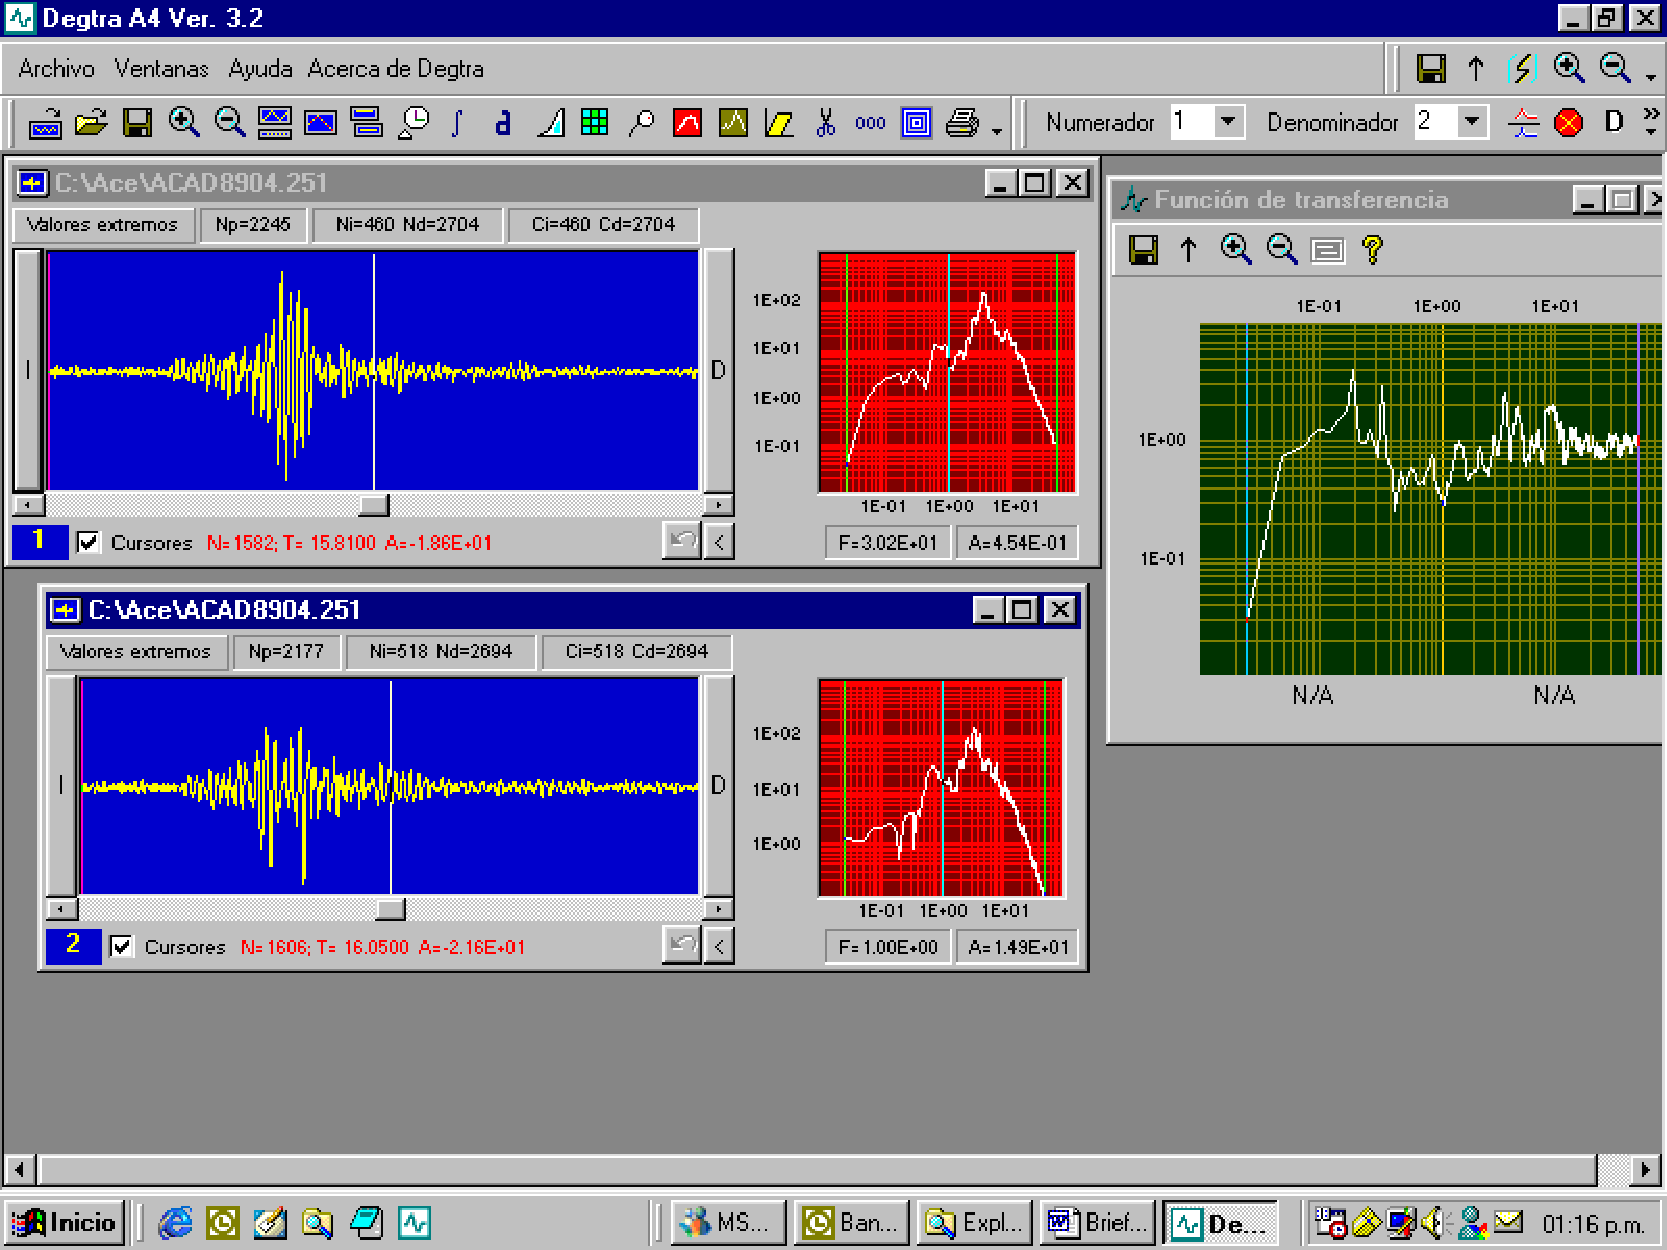
\includegraphics[width=0.9\linewidth]{fig/fig36}}
\caption{Example of DEGTRA A4.}
\label{fig:degtra}
\end{figure}

Degtra A4 accepts input ground-motion recordings written in several formats: simple ASCII or binary files, SEISAN format and the standard format of the Mexican Strong-Motion Database. 

The program has a nice and user-friendly interface, in which several time-histories can be manipulated at a time. It includes zoom-in/zoom-out capabilities that can be used if only a portion of a recording is of interest. 

There are two types of operations that Degtra A4 can perform using strong-motion recordings: operations involving a single recording and operations involving two recordings. 

Among the first group, the main functions are the following: 

\begin{itemize}
\item
Scaling. Multiplies the recording by a constant 
\item
Decimation. Decimates the recording by a user-given factor 
\item
Base-line correction: Includes several methods. 
\item
Differentiation: Numerical differentiation with respect to time. 
\item
Integration: Numerical integration with respect to time. 
\item
Computation of Arias' intensity. 
\item
Filtering: Includes high-pass, low-pass, band-pass and band-stop Butterworth filters, as well as Gaussian and Futterman filters. 
\item
Computation of elastic response spectra. Computes absolute acceleration, relative velocity, relative displacement and pseudo acceleration response spectra. 
\item
Computation of inelastic response spectra. Computes required-strength response spectra for fixed ductility demand of bilinear systems. 
\item
Computation of Fourier spectra. Computes and (optionally) smoothes FFT of a time signal. 
\item
Computation of response (acceleration, velocity, displacement) of elastic and inelastic (bilinear) single-degree-of-freedom oscillators. 
\item
Computation of the S-wave response of a soil column of given properties assuming that the time-history is the incident wave field at the base of the column. 
\end{itemize}


The main operations involving two recordings are: 
\begin{itemize}
\item[-]
 Spectral ratio. Computes the (Fourier) spectral ratio between two recordings. 
\item[-]
Odogram. Displays an X-Y parametric representation (time is the parameter) of two recordings, typically ground displacements, in order to observe particle trajectories. 
\item[-]
Addition/Difference. Computes the sum or difference of two recordings. This is useful, for instance, to identify rocking or torsional motions in buildings. 
\item[-]
Rotation: Rotates two components of the ground motion to arbitrary angles. 
\item[-]
Cross-correlation: Computes cross-correlation between two signals. 
\item[-]
Coherence: Computes coherence between two signals. 
\end{itemize}

Degtra A4 includes an on-line help file with details about the meaning of required parameters, techniques used, and use of Degtra A4 itself. It is available in two versions: one for Windows 2000 or lower and another for Windows XP. Installation is made with a typical Windows executable setup file. The distribution is found in directory SUP. 

Degtra A4 is currently in Spanish, English version in preparation. 

For questions please contact: 

\textbf{Mario Ordaz}, Institute of Engineering, UNAM \newline
mors@pumas.iingen.unam.mx 



\section{Calculating b-value, BVALUE}

\index{B-value}\index{BVALUE}

BVALUE is a program to make b-value plots using a NORDIC input file (also compact). A postscript plot file is generated. 

The questions are: 

\verbatiminput{include/bvalue.run}
\index{Maximum likelihood b-value} 
\index{Bvalue.out}
\index{Bvalue.eps}

The output file bvalue.out contains the same information in the same format as shown in the example above. The file can be used with other plotting programs to make 'nicer looking' b-value plots. An example is shown in Figure \ref{fig:b-value}. 

\begin{figure}
\htmlimage{scale=2.0}
\centerline{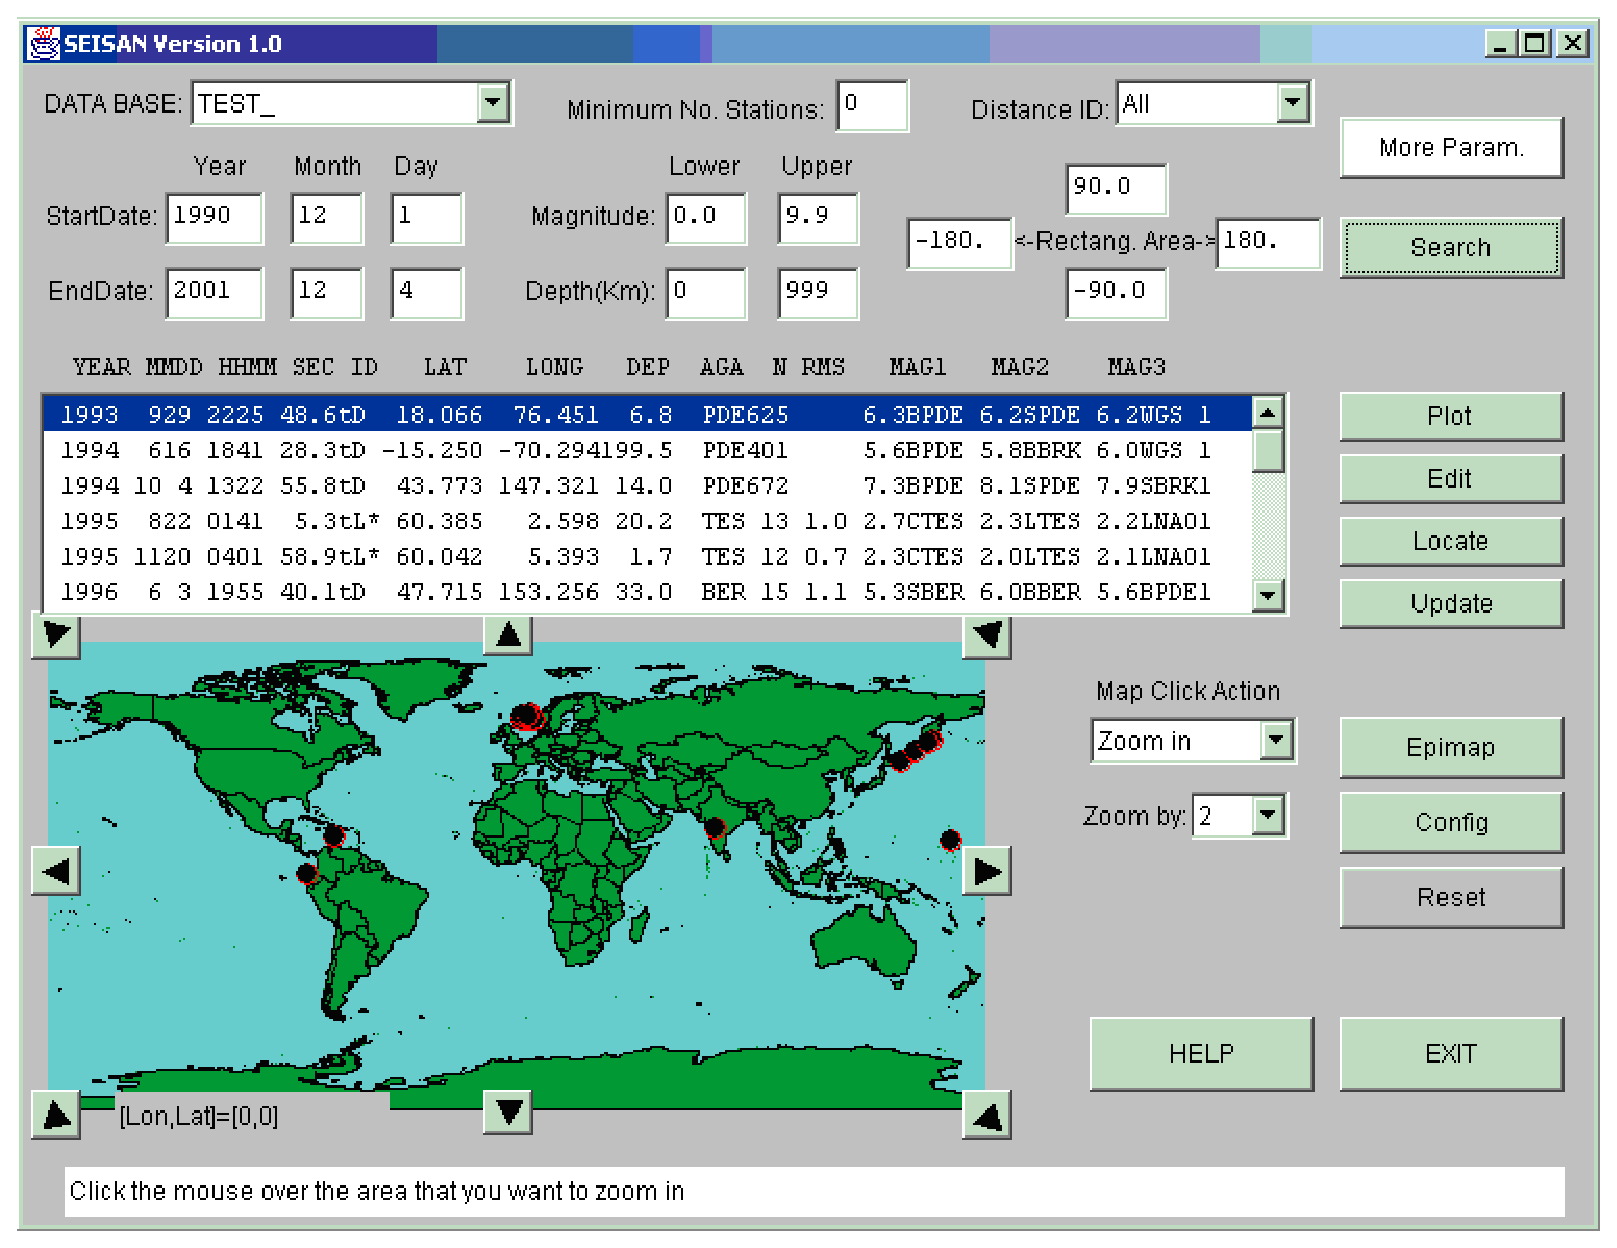
\includegraphics[width=0.9\linewidth]{fig2/fig6}}
\caption{
An example of a b-value plot. The bars are number of events and crosses the accumulated number of events. 
}
\label{fig:b-value}
\end{figure}




\section{Automatic phase picking, AUTO, AUTOPIC, AUTOSIG, CONDET}
\label{sect:auto-p-pick}
\index{Automatic phase picking}\index{AUTO} 


\subsection{AUTO and AUTOPIC}

%\textcolor{red}{lo-change:} 
AUTOPIC is a tool to automatically pick phases
on events registered into the database. 
	%\textcolor{red}{jh-change: The program uses an S-file as input. The waveform files must be listed in the S-file and the output of read phases are given in the S-file. The program can be started from EEV with command z, from the promatp line with command 'autopic sfile-name' or using program AUTO.}
The AUTO program will go through a series of events in the usual way using start time and end time and start AUTOPIC for each event.
If an event file (S-file) has any readings, the AUTO program will not reread in order to not destroy old picks. The automatic readings in the file are marked with an A after the weight column to indicate automatic pick. Each pick is evaluated by using the signal to noise ratio and an indication of the quality is given with the weight. The program will run on all waveform files given in an S-file. Each time the program runs, there is a file called auto\index{Autopic.out}pic.out containing information about the run. 
If there are any \index{3-component stations}3-component stations, an \index{Azimuth}azimuth will also be calculated, and the S-phase will be more reliable. 
The AUTOPIC program  can also be used from EEV by typing Z (will run program AUTOPIC). When it is used from EEV, there is always an output in the S-file, which will be grouped at the bottom of the file, making it possible to compare manual and automatic readings. THE S-FILE MUST THEN BE EDITED MANUALLY IN ORDER TO REMOVE DOUBLE READINGS. 
The program requires an input parameter file in the working directory or DAT with the name \index{AUTOPIC.INP}AUTOPIC.INP. The program will first look in the working directory. The parameters in that file are explained below. NOTE: The file is formatted, data must be in columns exactly as shwown and no tabs must be used.   
The program uses a 4-pole filter running one way. This might result in phases being picked a bit late. However, it seems more accurate than the earlier version where the filter run both ways and picks were often far too early. 
The program is made mainly by Bent Ruud. For more information about how it works, see \citet{ruud1988,ruud1992}. 
Description of parameters 

\verbatiminput{include/autopic.par}

Example of input file AUTOPIC.INP for AUTO 

%\verbatiminput{include/autopic.inp}
\verbatiminput{include/AUTOPIC.INP}



\subsection{AUTOSIG}

\index{Autosig}

AUTOSIG is a program to perform some automatic processing. The program 
includes routines for P-phase picking, determination of signal duration, amplitude determination, determination of spectral parameters \citep{ottemoller2003} and determination of distance type (local, teleseismic, noise). The program can still do with improvement. The input to the program can be either a parametric Nordic file (with one or several events) or waveform files. In both these cases, the output is written to the \texttt{autosig.out} file. Additional output files are \texttt{autosig.trace} and \texttt{autosig.err}, which will help to find potential problems. Alternatively, the program can also be started from EEV; the output is then directly written to the S-file. The input parameters are defined in the file \texttt{autosig.par}, which is located either in the DAT or the working directory.  

Following are descriptions of the automatic processing routines: 

P-phase picking:\newline
\index{P-phase picking} 
The phase picking is based on changes in the STA/LTA ratio. A band pass filter can be specified. The routine gives options to enhance the changes in the signal before computing the STA/LTA ratio. It is recommended to first remove the linear trend and then to compute the characteristic function which is given by y**2+k*(dy/dt)**2, which enhances changes in both amplitude and frequency content. Then the STA/LTA ratio is computed to detect changes in the signal. The routine can also compute the squared STA/LTA\index{STA/LTA}. When a change is detected (STA/LTA ratio above trigger level), it is tested whether the signal spectral amplitudes are significantly higher (factor of 2 in amplitude) than the pre-signal noise spectral amplitudes. This is done to avoid triggering on spikes. 

Signal duration:\newline
\index{Signal duration} 
The signal duration is determined by comparing the signal amplitudes with the amplitudes of the pre-signal noise. The duration is determined by the point from which the ratio of these amplitudes is lower than a given value. A filter is applied if specified in the parameter file. 

Amplitude: \newline
Routine finds maximum amplitude between two peaks. 

Spectral parameters:\newline
\index{Spectral parameters} 
The routine computes the displacement amplitude spectrum for P or S waves (see section \ref{subs:spec}) and, using either a converging grid search or a genetic algorithm determines the seismic moment and the corner frequency by minimizing the difference between observed and synthetic source spectra. The frequency band is determined by comparison with the pre-signal spectrum. The grid search is generally more cost effective and produces better results. The method is described in \citet{ottemoller2003}. The displacement spectrum is corrected for geometrical spreading and attenuation (both along the travel path and near surface). Therefore, the hypocentral distance has to be known. The time domain window for extracting the data from the trace can be given by either a group velocity (Vg=distance/travel time) window or a fixed window in seconds around the phase pick. 

Distance type: \newline
The routine determines whether the signal is from a local or teleseismic event, or noise. If signal spectral amplitudes are not significantly higher than pre-signal noise amplitudes, it is assumed that the signal is noise. Otherwise the amplitudes at two selected frequencies given by `DIST FREQ SELECT' are compared, the rules are (f1$<$f2): 

Spec signal amp(f1) - Spec noise amp(f1) $>$ Spec signal amp(f2) - Spec noise amp(f2): teleseismic \newline
Spec signal amp(f2) $>$ Spec noise amp(f2): local 

There are a few command line options that can be used to run autosig in non-interactive mode, 
syntax is 

\texttt{autosig -infile $<$filename$>$ [-spec on/off -phase on/off -clear on/off]}

where 

-spec on/off: determine spectral parameters if option given \newline
-clear on/off: remove phases from input S-file before start if option given \newline
-phase on/off: detect phases if option given \newline
-infile $<$file$>$: give name of input file, either S-file or waveform file \newline
-help: get help 

\textbf{Note}: When running the program the first time and the hypocenter location is not known, the determination of spectral parameters is not done. To run the determination of spectral parameters, the hypocenter location has to be given in the S-file. 

The meaning of most parameters in the parameter file is clear from the keyword. The spectral parameters are as described in the MULPLT section. Other parameters that need explanation are: 

\textbf{AUTO PHASE, AUTO SPECTRUM and AUTO AMPLITUDE}: Logical flag to activate phase picking, spectral analysis and amplitude reading, respectively (1. for true) 

\textbf{GA POPULATION SIZE}: Number of elements in the population, used only if SEARCH ALGORITHM is 1. 

\textbf{GA GENERATIONS}: Number of generations in one run, used only if SEARCH ALGORITHM is 1. 

\textit{Note: Increasing GA POPULATION SIZE and GA GENERATIONS will increase the computation time.}

\textbf{GRID NLOOP}: Number of loops in converging grid search for spectral parameters, used only if 
SEARCH ALGORITHM is 2. Resolution increases with every loop. 

\textbf{NGRID FREQUENCY}: Number of grid points in search for corner frequency, used only if SEARCH ALGORITHM is 2. 

\textbf{NGRID SPECTRAL AMP}: Number of grid points in search for spectral amplitude, used only if 
SEARCH ALGORITHM is 2. 

\textbf{NORM}: Norm for computation of residuals in spectral fitting can be set, however, tests show that 1 or 2 produce the same result, and generally default of 1 can be used. 

\textbf{SEARCH ALGORITHM}: Defines whether genetic algorithm (1) or converging grid search (2) should 
be used. Converging grid search is recommended. 

\textbf{SELECT PHASE}: Defines, which phase to use for spectral analysis, choices are: 0 for P by AUTOSIG, 1 for computed P arrival for given location, 2 for computed S arrival, 3 for P from s-file, 4 for S from s-file or 5 for S or P from s-file. 

\textbf{SEPCTRUM F LOW}: Lower limit of frequency band to be used.

\textbf{SPECDURATION CHOICE}: The time window for computation of the spectrum can be given either as a time window starting from the phase onset (0.) or can be defined by a group velocity window (1.). 

\textbf{SPECTRUM P LENGTH}: Duration in seconds of signal starting from P arrival. 

\textbf{SPECTRUM S LENGTH}: Duration in seconds of signal starting from S arrival. 

\textbf{SPECTRUM PRE LENGTH}: Duration in seconds of signal to be included prior to phase arrival. 

\textbf{GROUP VEL WINDOW P}: Range of group velocities defining time window to be used for P spectrum. 
Time window is given by (distance/group velocity) 

\textbf{GROUP VEL WINDOW S}: Range of group velocities defining time window to be used for S spectrum. Time window is given by (distance/group velocity) 

\textbf{STALTA NREC/REC}: There are two STA/LTA algorithms, recursive (0.) and non-recursive (1.). 

\textbf{STATION LINE}: One line with processing parameters for phase detection is given for each channel. The parameters are (also see example below): 

\verb|               |\textbf{STAT - station name}\newline
\verb|               |\textbf{COMP - component name}\newline
\verb|               |\textbf{STA - duration of STA}\newline
\verb|               |\textbf{LTA - duration of LTA}\newline
\verb|               |\textbf{RATIO - trigger ratio}\newline
\verb|               |\textbf{MINCOD - minimum coda required for trigger}\newline
\verb|               |\textbf{DTRLE - de-trigger level}\newline
\verb|               |\textbf{FILL - bandpass filter low cut}\newline
\verb|               |\textbf{FILH - bandpass filter high cut}

Example of the parameter file \texttt{autosig.par}\index{Autosig.par}: 

\verbatiminput{include/autosig.par}



\subsection{Detection program for continuous data, CONDET}

The CONDET \index{CONDET}program\index{Trigger} is a detection program works on data that is organized in a SEISAN continuous database or a BUD or SeisComp archive. It performs a detection process similar to real-time processing systems, but of course the data is already there. The program works in two steps, first to run a detector on a single channel, and second to detect events that are on more than a minimum number of stations. Possible applications are processing of data from a temporary deployment (e.g., aftershock monitoring, where continuous were recorded without event detection) and adjustment of detection parameters used in real-time monitoring. \index{Aftershock processing} 

The program has three built-in detection algorithms: 1) standard squared STA/LTA, 2) Carl Johnson's detector (that is for example used in the Earthworm processing system (\url{http://folkworm.ceri.memphis.edu/ew-doc/}) and 3) correlation with master event. The program writes out a list of detections (file \texttt{condet.out}, which gives station name, component code, trigger time and trigger duration), but also a batch file that can be used to extract the corresponding event data from the continuous data (file extract.batch). Note that wavetool by default takes data from all continuous databases listed in \texttt{SEISAN.DEF}. \index{Event detection} 

When started without any command line options, the program works on all stations/databases given by the STATION parameter. The output file has detections from all stations, and the extract.batch file has extract commands for all detections. This is all required if only one station is available. For more than one station, it is possible to search for times at which more than a minimum number of stations have triggered. This is done by starting the program with the command line argument `-net'. In this mode, the output file \texttt{condet.out} from the first run is used and the file extract.batch is overwritten. The extract script can now be used to get data for the network detected events. The script can be sources in Unix, under windows run comman in script or rename script to extract.bat and then run it. 
Condet is intended to run without questions and the parameter file condet.par must be in working directory. An example of condet.par is in DAT.

The input parameters are given in \texttt{condet.par}: 

STATION: give continuous database name, station and component code. If an archive, the data base name is not used. 
\begin{verbatim}
STATION                               LICOC       LICO  HH Z 
STATION                               LIGLC       LIGL  HH Z 
\end{verbatim}

The BASE TYP is SEISAN (blank), BUD (bud) or SeisComp(scp)
\begin{verbatim}
BASE TYPE                             scp 
STATION                               LIGLC       LIGL  HH Z 
\end{verbatim}

START DATE and STOP DATE: give time interval, can be larger than data availability 
\begin{verbatim}
START DATE          yyyymmddhhmmss        200802270000 
STOP DATE           yyyymmddhhmmss        200803122359 
\end{verbatim}

%\textcolor{red}{lo-change:
WAVEOUT: Set to 1. to write out waveform files with the original data and trigger channels.\newline
EXTRACT DURATION: Length of extraction window in seconds, used in \texttt{extract.batch}\newline
PRE EVENT TIME: Time to start extract before detection time in seconds, used in \texttt{extract.batch}\newline
INTERVAL: Length of data segment read at a time. The default is 60 minutes. \newline

DET ALGORITHM: choices for the detection algorithm are STA for squared STA/LTA, COR for correlation and CAR for Carl Johnson's detection algorithm \newline

MIN TRIG DURATION: Minimum duration the trigger level needs to be exceeded for \newline
MIN TRIG INTERVAL: Only allow for one detection within this time, given in seconds \newline
FILTER LOW: Low cut for bandpass filter \newline
FILTER HIGH: High cut for bandpass filter 

If DET ALGORITHM is STA: 

STA LENGTH: Short term duration in seconds \newline
LTA LENGTH: Long term duration in seconds \newline
TRIGGER RATIO: Ratio of STA/LTA required for trigger \newline
DETRIGGER RATIO: Ratio to detrigger \newline
FREEZE LTA: LTA can be frozen at time STA/LTA goes above 
TRIGGER RATIO, 1.=to freeze 

If DET ALGORITHM is CAR, see Earthworm documentation for details: 

CARL RATIO \newline
CARL QUIET 

If DET ALGORITHM is COR: 

CORRELATION MIN: Minimum correlation between waveforms of master event 
and the data required for a trigger \newline
MASTER WAVEFORM: Name of waveform file that is used as master event, 
the master event is cross-correlated against the continuous waveform data 

Network detection parameters: 

NET MIN DET: Minimum of detections required from different stations with time window given by
\newline
NET WINDOW SEC: Time window for network detection in seconds. 
NET MAX DELT SEC:
NET MIN RATIO:
EXTRACT DURATION: Duration(sec) of extract.



\section{Fault plane solution}
\label{sect:fps}
%\textcolor{red}{pv-change: 
SEISAN includes 
%\textcolor{red}{jh-change:
five programs for estimating the fault plane solution, 
FOCMEC, FPFIT, HASH (called hash\_seisan),EBEL and PINV. The programs are described below, 
they can all be called from EEV. Fault plane solutions can be plotted 
with EPIMAP (new from version 9.0), W\_EMAP (Windows only) and FOC 
(see below). The program GMTNOR also makes output which can be used with GMT.
In EEV fault plane solutions can be added manually to an event with commands inputfps or ifp.
%}

%
\subsection{FOCMEC}
\label{sect:focmec}

The program can be used to determine double couple earthquake focal 
mechanisms using polarities and/or amplitude ratios for both local 
and global earthquakes. The program also provides an interactive 
graphical display. The existing solution can be plotted without any 
station data or location being available, however if existing polarities 
should be plotted, the event must be locatable in order to calculate 
angles of incidence. Several solutions can be plotted on the same 
figure in order to compare solutions.

The SEISAN program FOCMEC provides the interface between the database 
and the program that determines focal mechanisms, which in SEISAN is 
the program FOCMEC\_EXE. This program is written by Arthur Snoke 
\citep{snoke1984} 
and distributed as part of the FOCMEC package 
(\url{http://www.geol.vt.edu/outreach/vtso/focmec}). 
FOCMEC\_EXE is identical to FOCMEC in Snoke's package and can be 
easily upgraded (unless formats are changed). Generally the user 
will use FOCMEC when working with SEISAN data, however, it is also 
possible to run the original version (see documentation by Snoke: 
INF/focmec.pdf).
%\textcolor{red}{lo-change: 
Before FOCMEC\_EXE is started the
user can optionally change the inputfile \texttt{focmec.run}.

\index{Polarity}

The program works with polarities and amplitude ratios. See the MULPLT section 
on how to read polarities and amplitudes.  Note that since amplitude 
ratios are used, there is no need to correct for instrument response 
provided the response is the same for the different components (within 5-10 \%).

Use of amplitudes

Amplitude ratios are computed from amplitude readings given in the S-file. While amplitude ratios can provide additional constraint on the solution, they should be used with caution. Ideally, the solution should be well constrained by polarities only, and then amplitude ratios can provide confirmation of a solution or help to select one of several equally good solutions. The principle behind the amplitude ratio method is that the effect of geometrical spreading will cancel out when forming the amplitude ratios of S and P waves (or SV/SH) of the same phase type, e.g. Pg and Sg. This leaves the following corrections  to be made  on the amplitudes before the ratios are calculated.

\begin{itemize}
\item
Calculate angle of incidence at the station and correct for the free surface effect.
\item
For local earthquakes, use the calculated travel time for a particular phase to correct for Q. Different Q for P and S can be used and the frequency used is the frequency of the maximum amplitude phase.
\item
For distant earthquakes, correct for $t^{*}$. Different $t^{*}$ for P and S can be used.  The frequency used is the frequency of the maximum amplitude phase.
\end{itemize}

The attenuation parameters have default values of:

\begin{displaymath}
\begin{array}{ll}
Q = 100 \times f^{1.0} & \textrm{for P and S-waves}\\
t^{*} = 1.0 & \textrm{for P-waves}\\
t^{*} = 4.0 & \textrm{for S-waves}
\end{array}
\end{displaymath}

Different values can be set in file FOCMEC.DEF, which can be located in DAT or working directory.

The observations to be made are:

\begin{itemize}
\item
Rotate the seismogram (if three component record) to get R and T components.
\item
Read maximum amplitude P-phase and corresponding period on Z, phase P.
\item
Read the  maximum amplitude S-phase (same type) and corresponding period on Z, phase (SV).
\item
Read the  maximum amplitude S-phase (same type) and corresponding period on H, phase (SH).
\end{itemize}

The wave type Pg/Sg or Pn/Sn has to be given when the amplitude is read. When reading on uncorrected seismograms, MULPLT will want a confirmation that the user wants to save uncorrected amplitudes, since, normally, all amplitude observations in an S-file are in nm. It is possible to filter the signals provided the same filter is used for P and S. Ideally, the amplitude observation should be made at a frequency below the earthquake corner frequency and consequently also the filter high cut frequency should  be below the corner frequency.

It is also possible to read amplitudes on the radial component. However, SV amplitudes and phases change rapidly around the critical angle and the amplitudes can therefore be unreliable (see INF/focmec.pdf for details). So, although SEISAN will use the amplitudes read on the radial component, it is in general not recommended to use them. Assuming reading on only Z and H, the following amplitude ratios are calculated:

\begin{itemize}
\item
SV/P
\item
SH/P
\item
SV/SH
\end{itemize}

In reality, the data only provides 2 independent ratios so ideally only 2 should be used. Since it is hard to know which 2 are the most reliable, SEISAN uses all. 

Phase names in SEISAN used for amplitudes for FOCMEC have the names AMPG, AMSG, AMPN and AMSN for direct and first arrival (refracted), respectively. For local earthquakes both PG and PN types can be used while for distant earthquakes only PN types can be used.

Polarity selection

Any P-phase (first letter of phase name is P) with a polarity (C or D) is used, like P, Pg, PP etc. For further processing in FOCMEC, C  is labeled C if phase onset is ' ' or I and '+' if phase onset is E. Correspondingly, polarity D is labeled D or -.   FOCMEC can also use polarities of SV and SH, but this has not been implemented in SEISAN.

Local earthquakes

Any P-phase can be used like Pn and Pg. When few polarities are available, it is an advantage to use both Pg and Pn since these phases have different angles of incidence. Polarities associated with other phases are not used. There is no check if a P-phase has been duplicated. \newline
Amplitude ratios must be determined from the same wave type for example Pg and Sg and the program will only form amplitude ratios from the same wave types.  While in principle it should be possible to use ratios determined from refracted waves, generally ratios determined only from direct waves are used since they are easier to identify and have larger amplitudes than refracted arrivals. Particularly the Sn is difficult to identify. This means that the amplitudes readings most often will be made within what is considered the maximum amplitude in the Pg and Sg wave trains. However, the polarity might be read on the first arrival which can be Pn or another refracted arrival. 

Distant earthquakes

Polarities of any P-phase can be used (but not pP since first letter is not P ). Using amplitudes require events with clear P and S phases and usually this means reading on broad band records. The amplitude phase names AMPN/SN are used to indicate first arrivals.


Program operation

The program makes a grid-search and finds how many polarities and amplitude ratios fit each possible solution. All solutions with less than a given number of wrong polarities and/or amplitude ratios within given error limits, are then written out and can be plotted. With a cursor, the user can then select the preferred solution, which can be stored in the input file or the database.  The program is intended to work from within EEV (option F), however it can also work independently (see below). The program uses an input file called \texttt{focmec.inp} (automatically generated). This is a Nordic format file. Direct waves have angle $>90$ and refracted arrivals angle $<90$ degrees. If the angle is $>90$, the polarity is plotted at an azimuth+180. If the user wants to use FOCMEC as a freestanding program, the angle of incidence information may have to be put in manually in a standard CAT-file, which is then renamed focmec.inp. This can be done automatically by FOCMEC if a \texttt{hyp.out} and corresponding print.out file is available. 
FOCMEC can also be used to convert angles, like dip, strike and rake to T and P-axis, simply say 'focmec a', where argument a stands for angles and you will be prompted for input.

%The program makes a grid-search and finds how many polarities fit each possible solution. All solutions with less than a given number of wrong polarities and/or amplitude ratios within given error limits, are then written out and can be plotted. With a cursor, the user can then select the preferred solution, which can be stored in the input file or the database.  The program is intended to work from within EEV (option F), however it can also work independently (see below). The program uses an input file called focmec.inp. This is a Nordic format file. The angle of incidence is put in column 58:60, format I3 (although from version 8 onwards, this information is part of the S-file). Direct waves have angle > 90 and refracted arrivals angle <90 degrees. If the angle is >90, the polarity is plotted at an azimuth+180. If the program is operated from within EEV, this information is automatically put in and the \index{Focmec.inp}focmec.inp file created. If the user wants to use FOCMEC as a freestanding program, the \index{Angle of incidence }angle of incidence information must be put in manually in a standard CAT-file, which is then renamed focmec.inp. This can be done automatically by FOCMEC if a \texttt{hyp.out} and corresponding \texttt{print.out} file is available.  FOCMEC can also be used to \index{Convert angles}convert angles, like dip, strike and rake to \index{T and P-axis}T and P-axis, simply say `focmec a', where argument a stands for angles and you will be prompted for input. 

\index{Focmec.inp}
\index{Angle of incidence}
\index{Convert angles}
\index{T and P-axis}

When the program runs, all amplitude information and corresponding corrections are listed:

\begin{verbatim}
============ FOCMEC ============
No FOCMEC.DEF file, use defaults

Q: Local: Qp= 100.0**1.00  Qs= 100.0** 1.0   Global: t*(P)=1.00  t*(S)=4.00

STAT  C PH       AMP    PER TRTIME   QCOR ANGINC ANGEMG Fcor   AZ  DIST
SNART Z PG      1582   0.16   12.6    1.2    100     79  0.6  301    77
SNART Z SG      9397   0.19   21.8    1.3    100     79 -0.3  301    77
SNART T SG     10577   0.09   21.8    1.3    100     79  2.0  301    77
MUD   Z PG        53   0.10   26.3    1.4     94     85  0.3  163   179
MUD   Z SG       197   0.15   45.5    1.7     94     85 -0.2  163   179
MUD   T SG       209   0.22   45.5    1.6     94     85  2.0  163   179
BLS5  Z PG       749   0.28   28.0    1.3     94     85  0.3  326   192
BLS5  T SG      1102   0.10   49.8    1.9     94     85  2.0  326   192
BLS5  Z SG       662   0.10   49.8    1.9     94     85 -0.2  326   192

 STAT  Ratio type  T     Amp 1    Amp 2  Fcor LogRat
 SNART SV(Z)/P(Z)  V      9397     1582   1.0   0.80
 SNART SH(T)/P(Z)  H     10577     1582   0.3   0.34
 SNART SV(Z)/SH(T) S      9397    10577   3.5   0.47
 MUD   SV(Z)/P(Z)  V       197       53   1.3   0.75
 MUD   SH(T)/P(Z)  H       209       53   0.2  -0.12
 MUD   SV(Z)/SH(T) S       197      209   7.5   0.87
 BLS5  SH(T)/P(Z)  H      1102      749   0.2  -0.45
 BLS5  SV(Z)/P(Z)  V       662      749   1.3   0.23
\end{verbatim}

%STAT  C PH       AMP    PER TRTIME   QCOR ANGINC ANGEMG   AZ  DIST
%SNART R PG       202   0.22   15.4    1.6     99     80    2    94
%SNART T SG       949   0.10   26.2    2.3     99     80    2    94
%SNART Z SG       656   0.15   26.2    2.3     99     80    2    94
%SNART R SG      1039   0.09   26.2    2.3     99     80    2    94
%MUD   Z PG        32   0.18   25.1    2.2     95     84  132   170
%MUD   T SG       231   0.10   43.5    3.9     95     84  132   170
%MUD   Z SG       164   0.08   43.5    3.9     95     84  132   170

%STAT  Ratio type  T     Amp 1    Amp 2  Fcor LogRat
%SNART SH(T)/P(R)  H       949      202   0.7   0.65
%SNART SV(Z)/P(R)  V       656      202   2.8   1.10
%SNART SV(R)/P(R)  V      1039      202   4.6   1.52
%SNART SV(Z)/SH(T) S       656      949   4.2   0.46
%SNART SV(R)/SH(T) S      1039      949   6.9   0.88
%MUD   SH(T)/P(Z)  H       231       32   0.2   0.35
%MUD   SV(Z)/P(Z)  V       164       32   1.2   1.05
%MUD   SV(Z)/SH(T) S       164      231   7.1   0.70

The abbreviations are STAT: Station code, C: Component, PH: Phase, AMP: Amplitude in count, PER: Period in sec, TRTIME: Travel time in sec, QCOR: Log Q-correction, ANGINC: Angle of incidence at the source, ANGEMG: Angle of emergence at the station, 
%\textcolor{red}{jh-change:
Fcorr: Free surface correction for this amplitude, 
Az: Azimuth from the event to the station, DIST: Epicentral distance in km., Ratio type (see text), T: indicator of ratio type, Amp1 and Amp2: The two amplitudes (count) in the ratio, Fcor is the free surface correction in the amplitude ratio (to be multiplied with ratio) and LogRat is the logarithm of the corrected amplitude ratio used.

Note that for station SNART, amplitudes were also read on the radial component so more then 3 amplitude ratios were used.

Following, the user get the choices:

%When the program runs, the following menu is put up: 

\begin{verbatim}
Stop                        (0)
Plot saved solution(s)      (1)
Plot new solutions          (2)
Plot selected solution      (3)
Find new solutions          (4)
-1, -2, -3 also plot station 
\end{verbatim}

\begin{enumerate}
\item
This is the solution(s) already stored in the data base (S-file). 
%The idea is that there should only be one prime fault plane solution. The prime solution has ' F' in the last two columns of the line. If any other character is put into column 79, the solution is not considered prime, however it will be left in the file when new solutions are generated.  There might be a need to plot several solutions in order to compare solutions. In that case the character in column 79 must be 'O'.
% \textcolor{red}{jh-change:
See secetion "Storing and selecting fault plane solutions" below.
%This is the solution(s) already stored in the data base (S-file). The rule is that there should only be one prime fault plane solution. The prime solution has ` F' in the last two columns of the line. If any other character is put into column 79, the solution is not considered prime, however it will be left in the file when new solutions are generated. There might be a need to plot several solutions in order to compare solutions. In that case the character in column 79 must be `O'.
\index{Fault plane solution, plotting several} 
\item
Plotting new solution after having used option 4 
\item
Plotting the selected solution after using option 4 \newline
Using e.g. -1 instead of 1, also plots the stations to 
help identify them on the plot, see Figure \ref{fig:focmec} 
\item
Starting a search for new solutions 

Option 4 gives the following information and questions: 

\begin{verbatim}
There are   10 polarity readings
Maximum number of allowed polarity errors or -1 to show best solutions only
\end{verbatim}

Depending on number of data values, 0-5 is a good answer. To let the program find the minimum number of polarity errors, type '-1', which is particular useful if there is a significant minimum number of polarity errors.

\begin{verbatim}
There are  8 amp ratio readings
Maximum number of allowed amplitude ratio errors
\end{verbatim}

Equivalent for ratios to 'Maximum number of polarity errors', however, error is defined by amplitude ratio error. Number of errors depends on number of observations. For 9 observations 1-2 errors is reasonable.

\begin{verbatim}
Maximum amplitude ratio error,  return for default of .2
\end{verbatim}

Give maximum allowed difference between observed and computed log amplitude ratio, default is 0.2, which often is a good value.

\begin{verbatim}
Degree increment in search
\end{verbatim}

%Number of polarity values: Number of polarities found for event with P-phases.  \newline
%Any P-phase can be used like Pn and Pg. When few polarities are available, it is an advantage to use both Pg and Pn since these phases have different angles of incidence. Polarities associated with other phases are not used. There is no check if a P-phase has been duplicated.  

%Number of amplitude ratios: Total number of amplitude ratios derived from amplitude readings in S-file. 

\end{enumerate}

%The program now asks:
%
%Maximum number of polarity errors: Depending on number of data values, 
%0-5 is a good answer. To let the program find the minimum number of 
%polarity errors, type `-1', which is particular useful if there is 
%a significant minimum number of polarity errors. \newline
%Maximum number of amplitude ratio errors: Equivalent for ratios to 
%`Max number of polarity errors', however, error is defined by 
%amplitude ratio error. \newline
%Maximum amplitude ratio error: Give maximum allowed difference between observed and computed amplitude ratio, default is 0.2. 
%
%Degree increment in search: Initially use e.g. 20 deg to make a fast 
%search, later use e.g. 5 deg to make a final solution. \newline

The program will now start the searching and write out on the screen (and in a file) the solutions which fit the requirement of number of misfits. The maximum number of solutions is limited to 100 as a default, or to the value defined by `FOCMEC MAXSOL' in \texttt{SEISAN.DEF}. At the end, the number of acceptable solutions is written out as well as the minimum number of bad fits. This can then be used for the next search. Now option 0 to 4 can be used again. 

When plotting the solution with option 2, the cursor comes up. Also, the solutions will be printed in text 
form to the screen, 
%\textcolor{red}{jh-change: 
see Figure 
\ref{fig:focmec}.
%, e.g.: 

%.\begin{verbatim}
%%.   Strike       Dip     Rake Pol: P      SV    SH   Rat Err  RMS RErr   RErr (All)
%. 358.0200   15.7900  -71.3200     1   0.0   0.0        0      0.25      0.25 
%. 358.1700   28.9000  -57.6200     1   0.0   0.0        0      0.09      0.09 
%.\end{verbatim}

The abbreviations are Pol: Number of polarity errors for P, SV(not used) and SH(not used), Rat Err: Number of ratio errors, RMS RErr: The RMS error for the ratios used, RErr (All): The RMS error for all ratios.

The polarities and amplitude ratios can be plotted on the focal sphere 
using the same convention as the original FOCMEC program, which is: 

\begin{tabular}{ll}
o = & compression \\
+ = & emergent compression \\
$\Delta$ = & dilatation \\
- = & emergent dilatation \\
V = & amplitude ratio SV/P \\
S = & amplitude ratio SV/SH \\
H = & amplitude ratio SH/P \\
\end{tabular}

%The last three fields Rat Err, RMS Rerr and Rerr refer to the number of ratio errors, the RMS error for the ratios used and the RMS error for all ratios, respectively. 

%When saving a solution, the same text field is included into the S-file. 

The user can select a preferred solution by moving the cursor near one of the letters T or P (T and P axis). By pressing T, the program will find the nearest T axis (same for P and nearest P-axis) and corresponding fault plane solution, which can be stored in the database and/or plotted with option 3. If no solution is to be selected, press q for quit. If a solution has been selected, the user will be asked if it is to be saved or not after selecting option 0. The saved solution goes into the 
\index{Focmec.out}
focmec.out and from there into the S-file (type F-line) in the database if FOCMEC is operated from EEV
%\textcolor{red}{jh-change: 
and the solutiosn will also be written to fps.out. 
%NOTE: The previous fault plane solution will be overwritten unless a character is written in column 79 of the fault plane solution line. If e.g. the last 2 characters are `OF', this solution remains in the S-file. 

When working from EEV, the event will always be located before the FOCMEC program starts up. In 
the Nordic format the solution is stored simply as 
\index{Strike}
strike, 
\index{Dip}
dip, 
\index{Rake}
rake and number of bad polarities (3f10.1,I5). Aki and Richards convention is used. In addition, the name FOCMEC will be written near the end of the line to indicate that the fault plane solution was made by FOCMEC. The other program, which can make a fault plane solution, is INVRAD (see EEV). The line type is F. 

The following files are created: 

\texttt{focmec.dat}: Input parameters to FOCMEC\_EXE. \newline
\texttt{focmec.log}: Log of the FOCMEC\_EXE run. \index{focmec.lst}\newline
\texttt{focmec.lst}: More details on solutions \newline
\texttt{focmec.out}: Gives input parameters and solutions \index{Focmec.eps}\newline
\texttt{focmec.eps}: A Postscript plot file of LATEST plot  \newline
\texttt{focmec.run}: Run parameters for FOCMEC\_EXE, you can re-run FOCMEC by `focmec\_exe < focmec.run' 

\textbf{Running FOCMEC independently of EEV and composite fault plane solution:}
\index{Fault plane solution, composite }

Locate event(s) with HYP, then give command focmec. The program then combines the files \texttt{print.out} and \texttt{hyp.out} \index{Hyp.out}to make the focmec.inp file and proceeds as usual. This is actually the way FOCMEC works from within EEV. However, if more than one event is located, FOCMEC assumes that all events shall be used in a composite solution, and focmec.inp will therefore contain the header from the first event and phase lines from all subsequent events. This is the easiest way to make a composite solution. 

NOTE, when running FOCMEC outside EEV, the fault plane solution is not put into the database (it does not belong to any particular event !), however it is written out in file focmec.inp 
%\textcolor{red}{jh-change:
and fps.out. 

Computer limitations: Total number of polarities must be less than the dimension of array DATA (parameter max\_data) for Nordic data (see file \texttt{seidim.inc} in INC directory). 

Figure \ref{fig:focmec} shows an example of a fault plane solution calculated with FOCMEC. 

\begin{figure}
\htmlimage{scale=2.0}
\centerline{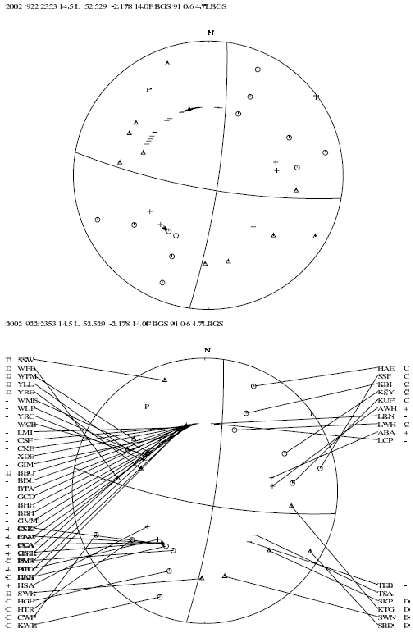
\includegraphics[width=0.9\linewidth]{fig/fig38}}
\caption{Top: An example of a fault plane solution plot. Symbols are explained 
in the text. Bottom: A fault plane solution also showing the stations with corresponding polarities. 
}
\label{fig:focmec}
\end{figure}


% {\color{red}jh-change:
\subsection{FPFIT}
\index{FPFIT}
\label{FPFIT}

This well known program, written by \cite{reasenberg1985}, 
%Reasenberg and Oppenheimer (1985), 
uses polarities to find one or several fps's (see manual fpfit.pdf in INF). 
Quoting the manual "Program FPFIT finds the double couple fault plane 
solution (source model) that best fits a given set of observed first 
motion polarities for an earthquake. The inversion is accomplished 
through a two stage grid search procedure that finds the source model 
minimizing a normalized, weighted sum of first motion polarity discrepancies". 
The weighted sum is expressed through the F-factor (0-1) given as output 
in S-file. A value below 0.5 is a good fit and a value of 1.0 is means 
a perfect misfit. A station distribution ratio STDR is calculated. 
Quoting the manual  "The station distribution ratio is 0.0 $<$ STDR $<$ 1.0. 
This quantity is sensitive to the distribution of the data on the focal 
sphere, relative to the radiation pattern. When this ratio has a low 
value (say, STDR $<$ 0.5), then a relatively large number of the data 
lie near nodal planes in the solution. Such a solution is less robust 
than one for which STDR $>$ 0.5, and, consequently, should be scrutinized 
closely and possibly rejected". This value is also written to the S-file.  
One advantage with FPFIT compared to FOCMEC is that formal errors are 
estimated and usually only one solution is given. The software is found at 
\url{http://earthquake.usgs.gov/research/software/} 
%http://earthquake.usgs.gov/research/software/index.php#

The original program FPFIT is left unchanged except for a minor gfortran adaption. FPFIT is an interactive program with many options for parameters stored in a parameter file and different data input formats can be used. In the SEISAN implementation, this has been simplified and a SEISAN driver program FPFIT\_SEISAN is used. This program converts the observations to an input file in hypo71 format, fpfit.dat, makes a parameter file with preset parameters, fpfit.inp and a run file fpfit.run to run the program. After running FPFIT\_SEISAN (either free standing or through EEV with command fp), it is possible to run the original program directly with command fpfit and test different FPFIT parameters, using fpfit.inp as a starting parameter file (default). It is then possible to interactively get information about the different parameters. The hardwired parameters essentially use default settings,  ensure the use of all data (e.g. no magnitude-distance restrictions) with the same weigh on all data. In addition, the following is set:

\begin{itemize}
\item[-] Search in as fine a grid as the program allows, one deg for fine search.
\item[-] Search for multiple solutions, not just the best. Gives an idea of uncertainty.
\item[-] Minimum number of polarities to attempt a solution is 6.
\end{itemize}
 
Run the program: In EEV, use command fp, first solution is written to S-file. The previous solution of FPFIT will be overwritten. FPFIT in SEISAN implementation can work with both global and local data, while the original FPFIT only works with local data. 
Outside EEV. See section on composite fault plane solution.

\begin{tabular}{|lp{4cm}|lp{12cm}|}
\hline
\multicolumn{2}{|l|}{Output files:} \\
\hline
fpfit.out & Details of inversion. In the FPFIT manual, this file is called
"Statistical summary file" \\ \hline
fpfit.fps & The fps solution etc. In the FPFIT manual, this file is called 
"Extended hypocenter summary card file" \\ \hline
fpfit.pol & Station and polarities used, see FPFIT manual \\ \hline
fps.out	 & The fps in SEISAN format in a cat file\\ \hline
\end{tabular}

Note: There is no check if polarities are read on Z-channel but it is required that the phase is P. 

% }

%{\color{red}jh-change: 
% 10 03 2011 jh  fix format of f-line, commant about w_emap bug
% 25 04 2012 jh  add command fq

\subsection{HASH}
\index{HASH}
\label{HASH}

This program \citep{hardebeck2002,hardebeck2003} determines fault plane 
solutions using P-polarities and amplitude ratios as input, just like 
the FOCMEC program. The P-amplitude 
$A_P=\sqrt(A_r^2+A_z^2)$
 and the S-amplitude 
$A_S=\sqrt(A_{sv}^2+A_{sh}^2)$
 where A 
is amplitude, r is radial, z is vertical, sv is SV, and sh is SH. 
The free surface correction is not built in, but replaced by a fixed 
factor per station, which has to be determined independently. In order 
to simplify the input, the free surface corrected amplitude ratios 
from FOCMEC are used as input for HASH. The program was modified 
to use only SH and by using the free surface corrected P on the Z-component, 
the assumption is made that $A_p = A_z(P)$. Thus only one amplitude 
ratio is used for each station (SH to P). HASH returns solutions with 
less than a given number of polarity errors and average amplitude 
errors less than a given limit. If no solutions are found, error limits 
are increased and normally many solutions are returned. Using this, 
an estimate of the best solution is made and likely errors calculated. 
The advantage with HASH is that it finds one or a few best solutions, 
while for FOCMEC the user must select one among many. Also HASH will 
not completely change the solution by one wrong amplitude ratio, since 
the average of the amplitude errors is used as selection criteria and 
not a single amplitude. FOCMEC does not give any estimate of the errors 
in the solution. HASH calculates an estimated error; however that requires 
an input where each event has been located with e.g. 10 different likely 
input models and all data is used as input in order to get estimate of 
fault plane solution uncertainties generated from the model. This was 
not done in the SEISAN implementation so only the error estimated from 
the spread in solutions is used.  This might lead to smaller error estimates 
as compared to the original HASH implementation. The SEISAN HASH implementation 
is a simplified implementation compared to the original HASH with many 
parameters hardwired, see hash\_seisan.for for implementation details and 
changes. Like FPFIT, the F-fit function is calculated (called weighted 
fraction of polarity misfits) and similarly the station distribution 
ratio (see FPFIT). Both values are given in S-file as well as the average 
amplitude error. For more information, see the HASH manual hash.pdf 
and FPFIT manual fpfit.pdf in INF. The software is found at 
\url{http://earthquake.usgs.gov/research/software/index.php}.
%http://earthquake.usgs.gov/research/software/index.php. 
HASH does 
not estimate errors in strike, dip and rake but errors in fault plane and auxiliary plane (degrees). 

Running HASH from EEV

Polarities and amplitudes are picked like for FOCMEC. When running the program, the amplitudes are corrected like for FOCMEC (actually done by FOCMEC) so the Q-correction will use the Q-relation given in focmec.def (see FOCMEC description above). The same output, as for FOCMEC, with the available amplitudes, their ratios and corrections will be shown and the control is the handed over to HASH. The questions are:

\begin{verbatim}
  Grid angle for focal mech. search, enter for def 2            Comment: Smallest is 2

  Max number of polarity errors                                 Comment: No default
1
  Max average error in amp rat, log10, def 0.2                  Comment: default 0.2 selected

  Enter angle for computing mechanisms probability, def is 60   Comment. Default 60 deg. Sel.

  Enter probability threshold for multiples, def is 0.1         Comment: Default 0.1 selected
\end{verbatim}

Now is following the FOCMEC amplitude information, not shown $\ldots$

\begin{verbatim}
 Number of polarities is                      :    11
 Number of amplitude ratios is                :     5
 Minimum number of polarity misfits overall   :     0     
 Minimum average amplitude error overall      :  0.13
 New number of pol. misfits inc. extra is     :     1
 New average amp limit inc. extra             :  0.23
 Minimum average amplitude error for pol ok   :  0.27
 New average amp limit is                     :  0.37
 Number of solutions found                         92

 Strike,dip,rake               197.3    66.5  -157.4
 Fault+aux plane uncertainty    23.2    10.3
 ================================
\end{verbatim}

Explanations on input:

The "mechanism probability" is the probability that the real mechanism 
is "close" to the preferred mechanism, within "angle for computing 
mechanisms probability" where angle define "close." If there are 
clustered outliers, alternative solutions (or "multiples") are found 
based on those outliers. You can set the minimum probability for the 
multiples (i.e. ignore multiples with a low probability.)

Explanations on output:

\verb|Minimum number of polarity misfits overall|: 
Minimum number of wrong polarities for anyone of the grid points 
disregarding amplitude fit. This is the number of polarity errors 
to find a solution without amplitudes.   \newline
\verb|Minimum average amplitude error overall|: The minimum average log error for any grid point disregarding errors in polarity.\newline
\verb|New number of pol. misfits inc. extra is|: The new limit for polarity errors.     \newline
\verb|New average amp limit inc. extra|: Based on the above, a new amplitude ratio error limit is set.\newline
\verb|Minimum average amplitude error for pol ok|: The new error limit considering polarities within limit.\newline
\verb|New average amp limit is|: In order to get sufficient solutions, the amplitude error limit is increased to this value.\newline
             
Output files:
Hash\_seisan.out: A summary of the solutions(s).\newline
Fps.out: The solution(s) in SEISAN format.

\textbf{Storing and selecting fault plane solutions: Format errors estimates and quality.}

The fault plane solutions are stored in the S-file. Different programs give somewhat 
different parameters and sometimes the same output field is used for 
different parameters. Some programs give strike of dip instead of 
strike of fault plane, but values used in SEISAN are converted to 
strike of fault plane. Each program is indicated with its own name 
like "\verb|HASH     F|" at the end of the F-line. If no characters are 
written in the blank space, any new solution will overwrite the old 
one. However if anything is written like "\verb|HASH    1F|", any new solution 
will create a new line in S-file. This is also the case if a quality 
indicator is written (see below). An example is:

\begin{verbatim}
     158.0      53.1    -156.4  7.0  3.8      0.30 0.57 0.76      FCF HASH     F
   39.2900   66.3900  -63.6500                          0.13  2 1 FCF FOCMEC   F
      42.0      68.0     -62.0  7.0  5.0  3.0  0.1  0.2           FCF FPFIT  A F
      18.7      67.8     -63.3                                4   FCF PINV     F
\end{verbatim}

In this example, there are 4 solutions made by the 4 programs and the solution made by FPFIT has been selected as a prime solution with quality A. The content and format is: 

\begin{verbatim}
Type F Line (Optional): Fault plane solution 

Columns Format Description

  1:30 3F10.0 Strike, dip and rake, Aki convention
 31:45 4F5.1  Error in strike dip and rake (HASH), error in fault plane and aux. plane (FPFIT) 
 46:50 F5.1   Fit error:  FPFIT and HASH (F-fit)
 51:55 F5.1   Station distribution ratio (FPFIT, HASH)
 56:60 F5.1   Amplitude ratio fit (HASH, FOCMEC)
 61:62 I2     Number of bad polarities (FOCMEC, PINV) 
 64.65 I2     Number of bad amplitude  ratios (FOCMEC)
 67:69 A3     Agency code
 71:77 A7     Program used
 78:78 A1     Quality of solution, A (best), B C or D (worst), added manually
 79:79 A1     Blank, can be used by user
 80:80 A1     F
\end{verbatim}


\verb|Quality indicator|: The indicator can be any character, but usually A to F is used with A as the best. It is up to the user to manually assign a quality indicator. Events can later be selected based on quality indicator. Programs SELECT and FOC use quality indicators. The quality indicator as well as the selection of the prime solution can be select by command fq in eev. An example is given below:

% jh change, following should be courier, smaller font

  Fault plane solutions for this event
 1  180.3      55.1    -123.7  5.0  4.4      0.04 0.67 0.38      SJA HASH   A
 2 6.1000   48.4400  -48.0700                               2    SJA FOCMEC
 3  191.0      51.0    -110.0                                    SJA DREGER
 4  185.0      48.0    -121.0                                    HRV CMT    A
  Give fps number to be prime solution, enter for no change




\textbf{Composite fault plane solutions}

A composite solutions means that data from several events, suspected to have the same fps, will be used together. Composite solutions can be useful if little data is available. All programs except INVRAD can be used for a composite solution. Composite solutions must be calculated outside EEV and the solutions therefore do not become part of the data base. Both amplitudes and polarities can be used. Local and global data can be used. The procedure is:

\begin{itemize}
\item Select events to be used together in one cat file, e.g. by using SELECT.
\item
Locate the events with HYP, there will then be a hyp.out and a print.out, which are used as input for the composite solution.
\item Start one of the 4 fps programs: FOCMEC, PINV, FPFIT\_SEISAN or HASH\_SEISAN. The usual questions will come up. 
\item The solution(s) will be written in the individual program output file. The solution(s) will also be written to the cat-file fps.out in standard SEISAN format. For each run of a program, the solutions accumulate in fps.out. This can be used to compare solutions from different programs, see FOC. An example of the plot is seen in Figure \ref{fig:foc}. To plot the observations, put in solution
in hyp.out and plot with FOCMEC.
\end{itemize}
 
\begin{figure}
\htmlimage{scale=2.0}
\centerline{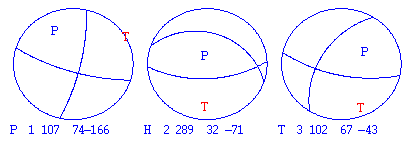
\includegraphics[width=0.9\linewidth]{fig/foc}}
\caption{Using FOC to plot solutions from fps.out. The program used 
for each solution is given with a one letter code: P: PINV, F: FOCMEC, H: HASH and T: FPFIT.}
\label{fig:foc}
\end{figure}


\textbf{Which program to use}

The different programs all have advantages and disadvantages. FOCMEC uses the most data since it can use more amplitude ratios than HASH but it might be difficult to find the 'correct' solution since a small change in input limits might make a large change in output. If a few of the amplitude ratios are very wrong, an unrealistic high ratio limit must be used and many errors allowed. This problem is avoided by using HASH since the limit is the average amplitude ratio error and not the number of errors. If only working with polarities, all 4 programs can be used. PINV gives a very quick solution which can be used as an indication of a possible best solution, however for final results one of the other 3 programs should be used. It is often a good idea to compare the results from the different programs. Ideally they should all give the same result, but there will be difference due to different methods used and different data, however if solutions are very different, the solution might not be very stable. It is easy to compare the solutions. Run each program in EEV, then plot using command fo. Each solutions will be plotted in a different color, see Figure \ref{fig:fps-compare}. If doing composite solutions, use program FOC with input from fps.out. 

\textbf{SLICK, inversion of fault plane solutions to get best stress tensor}

This program is part of the Slick package doing the following quoting the author \cite{michael1984} "The slick package uses fault slip data (either field observations or from focal mechanism) to find the stress tensor that best explains the observations. Inputs are the orientation and slip direction of a set of fault planes. Outputs are the orientation and shape of the stress ellipsoid, including confidence regions, and statistics used to judge the success of the inversion. This method uses the linear inversion algorithm and non-parametric bootstrap statistics". The software is available at 
\url{http://earthquake.usgs.gov/research/software/index.php}. 
%http://earthquake.usgs.gov/research/software/index.php. 

In SEISAN, only the inversion part has been implemented so the error analysis is missing. Program SLICK can be run as a separate program, but is normally run as part of FOC which prepares the input for SLICK and plots the output.  The method is explained in \cite{michael1984} where also examples are given with data available at the above web site.
Running SLICK: slick "file", where "file" is a file with strike of dip, dip and rake. An example input file is:

\begin{verbatim}
Strik dp     Dip    Rake
   203.0    51.0   137.0
   280.0    85.0  -161.0
    ...
\end{verbatim}

Note that in SEISAN, strike of fault plane is used so the strike of the dip is strike of the fault plane+90 degrees. The output is "file.oput" which gives the found stress tensor and the fit to the data, for details see \cite{michael1984}. The stress tensor has a corresponding slip angle, (average slip) and for each event the difference in slip angle for the individual event and the average slip is calculated as well as the average difference and standard deviation.  When running SLICK with FOC, an input file foc.slick is made for selected events (making the corrections to strike of slip) and the output file is foc.slick.oput. FOC also plots the direction of maximum compressive stress s1, minimum compress stress s3 and null axis s2. In the example below s1 has max value of 0.68 and strike and dip are 19 and 34 respectively. S3 has strike and dip of (113, 5) and s2 (-149, 56) respectively. The average fit angle is 59 with a standard deviation of 51, a bad fit.

\begin{verbatim}
stress tensor is:
-0.290526  0.236582  -0.146602  
0.236582  0.293028  -0.438347  
-0.146602  -0.438347  -0.00250278  
eigenvalue   vector: E,N,UP,direction,plunge
0.686771  -0.273399  -0.784281  0.556917  19.205739  33.820430
-0.37516  -0.917882  0.385856  0.0927811  112.725966  5.320093
-0.31161  0.287656  0.485818  0.82537  -149.270892  55.589101
variance= 0.283314
phi value= 0.940156

dip direction, dip, rake, fit angle, mag tau
  203.0     51.0    137.0    166.4    0.11
  280.0     85.0   -161.0    167.9    0.19
   ...
   13.9     68.1    -85.7     11.0    0.46
   14.0     70.0   -130.0     33.3    0.48
fit angle mean= 59.156784 standard deviation= 51.527176
for f=0.8 I= -2.242677 , std. dev.= 1.609795 D norm= 0.248640
avg tau=xx , std. dev.= xx
\end{verbatim}


For a complete stress analysis it is recommended to also do the error analysis using the complete slick package or e.g. the program ZMAP (not a SEISAN program, uses MATLAB, found at 
\url{http://www.earthquake.ethz.ch/software/zmap/ftp}).  
%http://www.earthquake.ethz.ch/software/zmap/ftp).  
FOC writes a file which is formatted for input to ZMAP. However doing stress analysis as implemented in SEISAN gives a good impression of the consistency of the fault plane solutions in a particular area. It is recommended that at least 10 events are used for inversion.
 

Plotting fault plane solutions

There a 4 ways of plotting fault plane solutions in SEISAN:  Through EEV (a single event), program FOC (many events), program EPIMAP (many events) and W\_EMAP (many events). The input file is in all cases a CAT-file. In addition, using program SEIGMT, a file to be used with GMT is prepared, however the use must make his own script. Only through EEV is it also possible to plot the observations.

Using EEV\newline
Command fo will plot all events in S-file. This can be a useful ways of comparing solutions obtained by different programs, see Figure \ref{fig:fps-compare}.

 

\begin{figure}
\htmlimage{scale=2.0}
\centerline{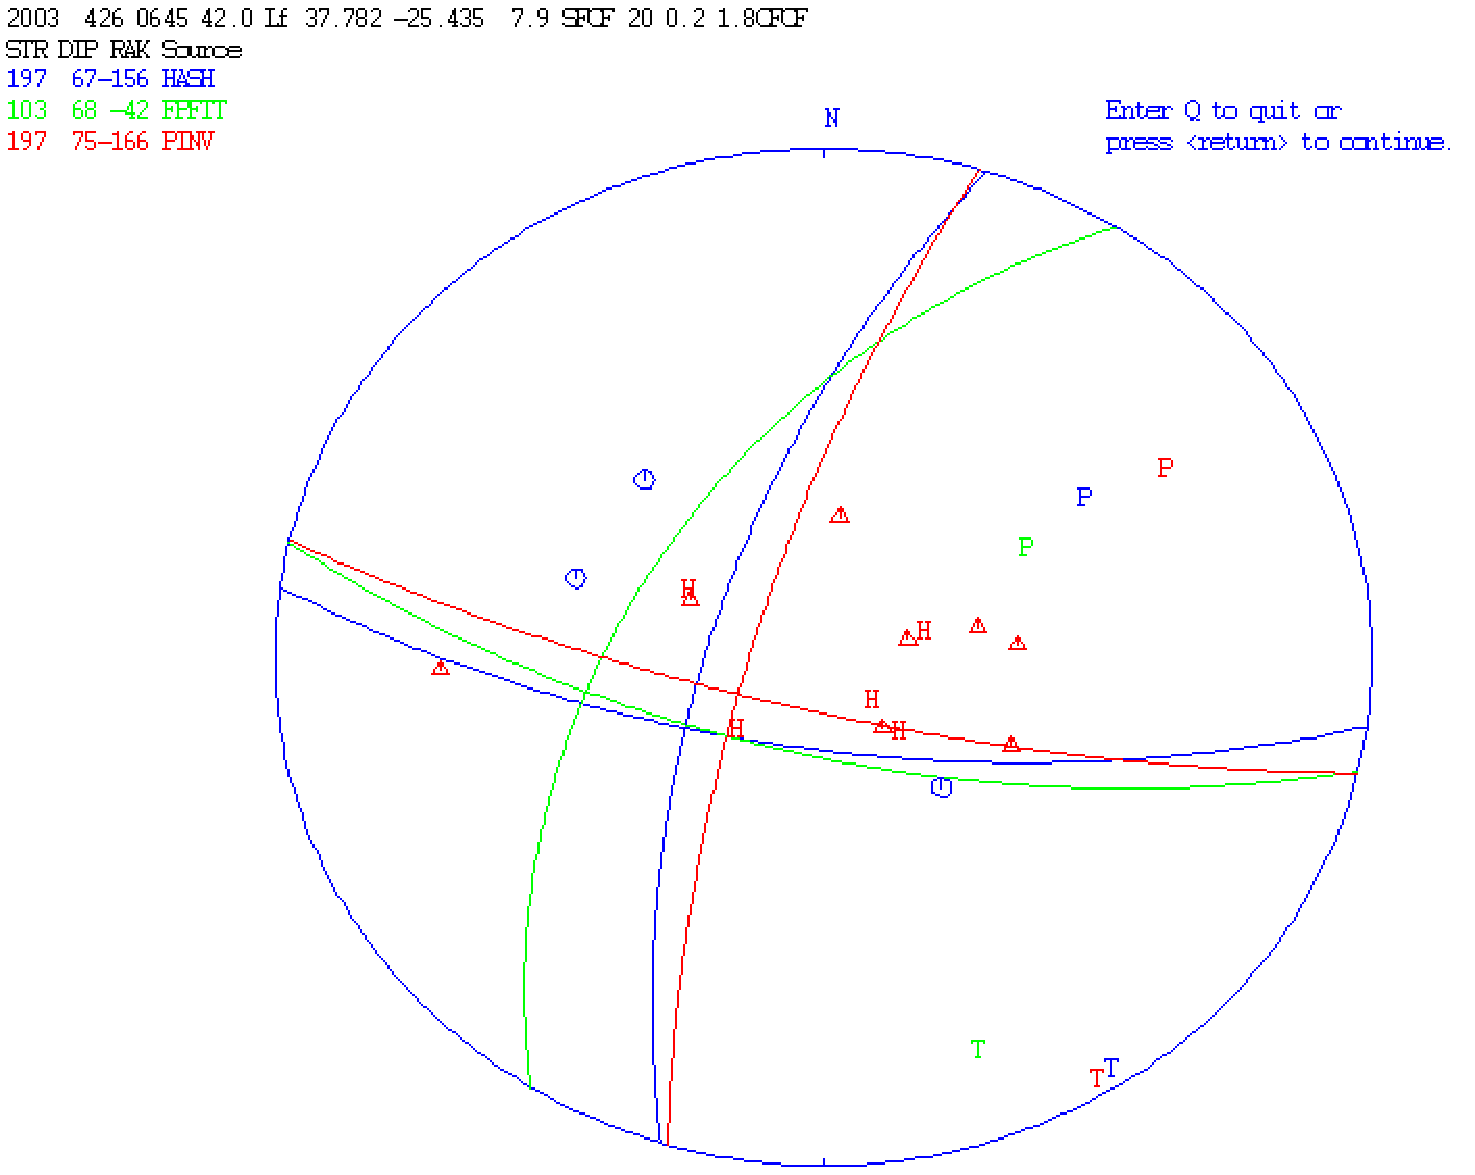
\includegraphics[width=0.9\linewidth]{fig/fps-compare}}
\caption{Compare fault plane solutions from different programs. For explanation of symbols, see FOCMEC.}
\label{fig:fps-compare}
\end{figure}


Using FOC\newline
See under FOC for how to run the program, see page
\pageref{page:foc}.
The plot is seen in Figure \ref{fig:foc}.


 
\begin{figure}
\htmlimage{scale=2.0}
\centerline{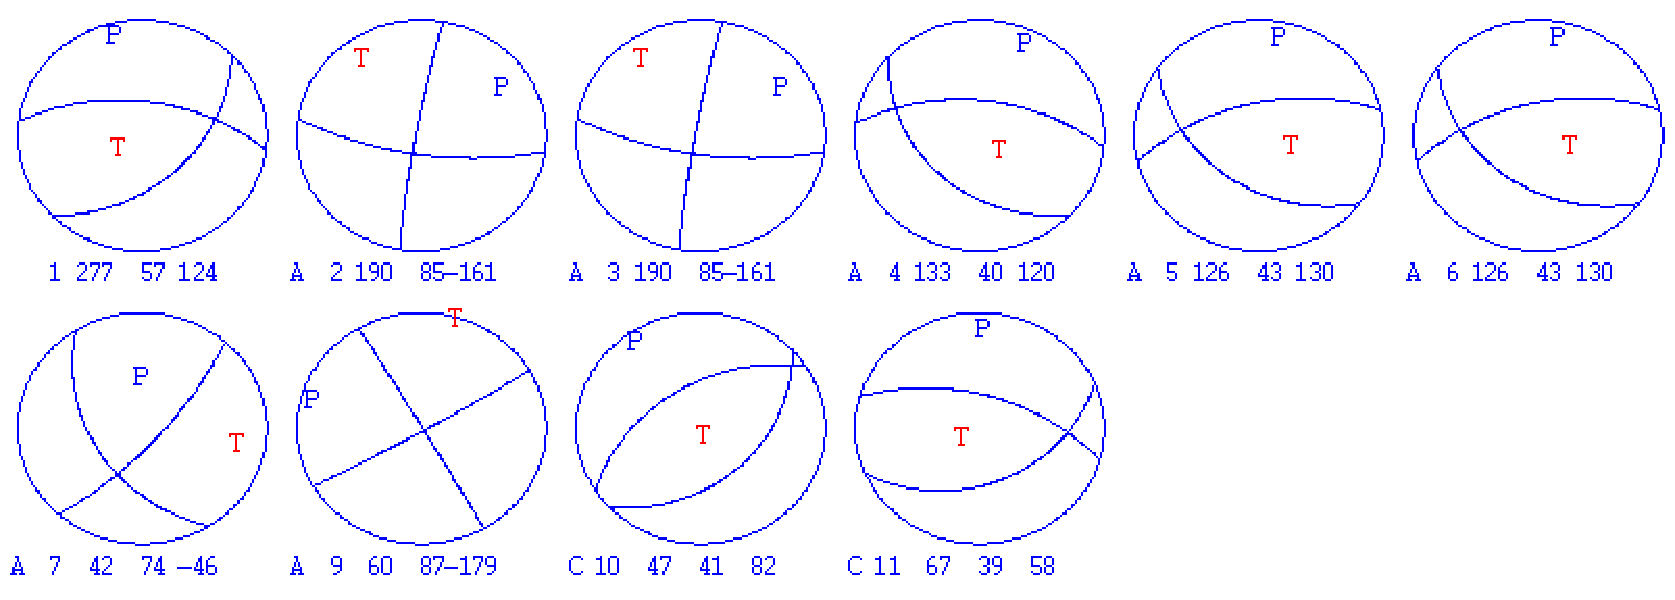
\includegraphics[width=0.9\linewidth]{fig/fps-many}}
\caption{Example of plotting many solutions. Each solution is given with number, the fault plane solution and the quality (A-E). Up to 24 solutions can be plotted on one page.}
\label{fig:fps-many}
\end{figure}


W\_EMAP (Windows only) plots the solutions as seen in Figure \ref{fig:fps-twomaps}. 
In this case the simplest is to give command w\_emap file, where file 
is the CAT file with fault plane solutions. See W\_emap manual in INF. 
NOTE: Some versions of W\_EMAP plots some of the fault plane solutions 
with inverted color e.g. inverse fault becomes a normal fault).

  

\begin{figure}
\htmlimage{scale=2.0}
\centerline{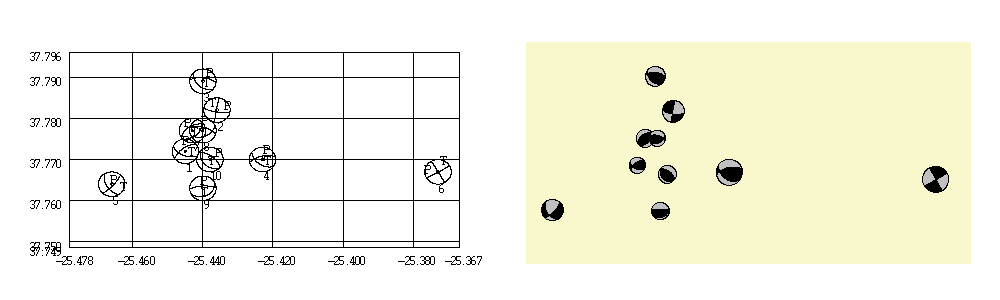
\includegraphics[width=0.9\linewidth]{fig/fps-twomaps}}
\caption{Plotting many fault plane solutions. Left: Using W\_EMAP. Notice that the colors in the solutions are inverted compared to normal practice. Right: Using EPIMAP. The data for the two plots is the same.}
\label{fig:fps-twomaps}
\end{figure}


The EPIMAP plot for the same events is shown in Figure \ref{fig:fps-twomaps}. See EPIMAP for more explanation. EPIMAP can also plot the fault plane solutions in a section, the solutions are still seen in the horizontal plane.


\textbf{FOC}
\label{page:foc}.

FOC is a program doing different things with fault plane solutions given in a CAT-file: Converting data to other formats, plotting many solutions, running the SLICK program and displaying the results, plot P and T axis for many events and make statistics of polarities. The input is:

\begin{verbatim}
foc
 Give input file
collect.out
 Quality, ABC.., up to 5 chars, enter for all
AB                                            Comment: Different qualities can be selected
 Cumulative(c) or individual misfit(def)      Comment: See later

 Plot all solutions selected (Y=enter/n)      Comment: Analysis can be done without plotting all
N
\end{verbatim}

The plot of the many fault plane solutions is seen in Figure \ref{fig:fps-slick}. 
After plotting the fault plane solutions, a plot comes up plotting 
the location of the P and T axis and the results from SLICK, see Figure \ref{fig:fps-slick}.

 
\begin{figure}
\htmlimage{scale=2.0}
\centerline{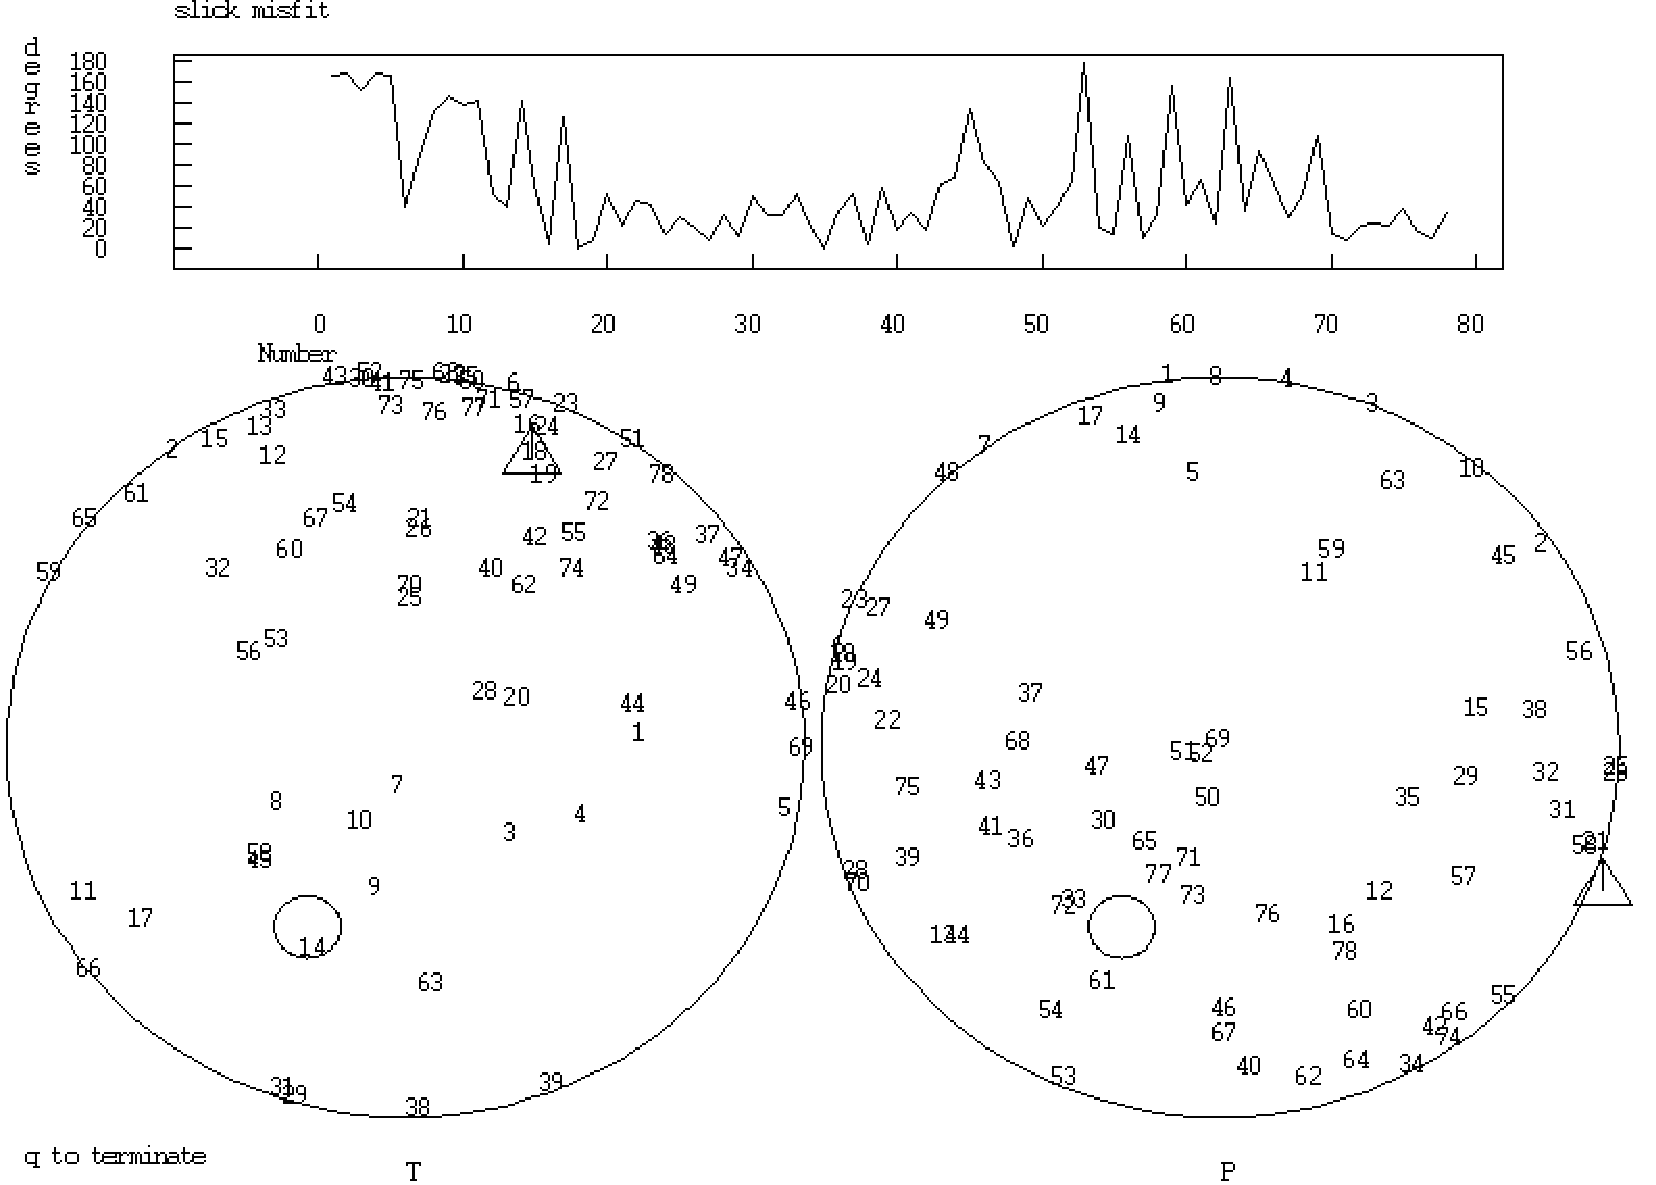
\includegraphics[width=0.9\linewidth]{fig/fps-slick}}
\caption{Left: The position of the T-axis given by the event numbers. The triangle is the SLICK minimum compressive stress direction and the circle is the null axis. Right: Corresponding for P-axis and the triangle is now the maximum compressive stress direction. Top: The misfit for each event as a function of event number. This figure can also show the cumulative misfit, see example run of FOC.}
\label{fig:fps-slick}
\end{figure}


Output files:\newline
Foc.out: P and T axis for all events, can be used as input to make rose diagrams.\newline
Foc\_events.out: The events used based on quality selection\newline
Foc\_pol.out: Statistics of polarities:

\begin{verbatim}
Stat     C    D
AZ05     3    2
MESC    18   60
VIF0     5    2
MIRA    10   32
VIF     44   19
LFA     52   18
PRCH    36    6
PVER    26    3
FRA0     0    2
AZ07     1    1
.
.
SET2     3    0
PSAN     1    3
 Sum of maximum number of polarities         570
 Sum of minimum number of polarities         158
\end{verbatim}

For each station the different polarities are counted and a sum of the consistent polarities are given at the end.
Foc.zmap: Input file in format used by ZMAP, notice direction of slip is used instead of strike of fault, see SLICK.\newline
Foc.slick and foc.slick.oput: See SLICK.

NOTE: FOC uses the first instance of the fault plane solution found in file for a particular event.

%}

%\textcolor{red}{lo-change:}
\subsection{Moment tensor inversion program, PINV}
\index{PINV} 
\label{PINV} 
\label{page:pinv} 

This program makes a preliminary best fault plane solution based on 
polarities and is intended as a help to other methods of fault plane 
solution. The original program was written by Suetsugu and some 
information is found in \citep{suetsugu1998}.  A copy of this report, 
which also gives general information about fault plane solutions, 
is available as foc.pdf at 
\url{http://iisee.kenken.go.jp/lna/?mod=view\&cid=S0-250-2007}

To run the program from EEV:

Command \texttt{pi} will locate the current event and then start PINV (stands for P-inversion).  PINV is hardwired to use hyp.out as input file and it will use all polarities from P-phases (capital P as the first letter). The result of the inversion is written out on the screen and in file pinv.out.  The strike, dip and rake and number of wrong polarities is also written to the S-file provided at least 5 polarities are available, however PINV will make an inversion with any number of polarities and write the result to the screen. In the S-file, the result is written as an OF-line giving the source of the inversion as PINV. A new inversion will overwrite the previous solution. This means that a PINV solution will be additional to the solution given by the F-line and therefore not considered as prime. It is also possible to directly compare the solution to the solution obtained by FOCMEC.

To run program outside EEV.

The program can run with one or many events (composite solution). First locate event(s) with HYP, then give command ‘pinv’ and the inversion is made. All polarities in the hyp.out file are used. The result only goes the screen and pinv.out.

Principle of operation:

Moment tensor inversion can be done most simply using amplitudes as observed on the focal sphere. In PINV, polarities are considered to be amplitudes of +1 or -1 corresponding to compression and dilation, respectively. This is a gross oversimplification since there will be large variation of real amplitudes over the focal sphere. This input data of ‘amplitudes’ is then inverted to get the moment tensor under the restriction of finding a single double couple. Despite the simplification, the advantage of this method is that it very quickly gives a ‘best’ approximation to the fault plane solution. This “best“ solution, particularly with few data, might be just one of many possible (see FOCMEC), but it serves to give an idea of a possible ‘best’ solution and it is in general consistent with the observations \citep{suetsugu1998}.  Unfortunately PINV does not give an error estimate to judge how reliable the solution is. It is therefore not recommended to use PINV to obtain prime fault plane solution, but rather as a help to select a solution when using FOCMEC unless much well distributed data is available.
In some cases, FOCMEC will find a solution where all polarities fit, while PINV will get a similar solution with some polarity errors. This can be explained by PINV using the assumption of  +1 and -1 amplitudes and thus an overall fit to amplitudes near nodal planes might be difficult. The original  input  to the PINV program has an option to give zero amplitude of observations judged nodal, however in our experience it is hard to judge if a first polarity is nodal or just has a small amplitude du to path (e.g. Pn) so this option has not be included.  

An example of a run is:

\begin{verbatim}
Number of data used for inversion=  8
Absolute pseudorank tolerance     0.001210          Pseudorank   5
Strike, dip, rake           72.3      38.9      34.6
Consistent data:     8
Inconsistent data:   0
\end{verbatim}

There were 8 observation which all fitted. The pseudorank indicates how many parameters can be determined in the inversion. In this case 5 since there are 8 observations. If less than 5 observations, the pseudorank will be less than 5.  The Absolute pseudorank tolerance  is a measure of the fit.



\subsection{Moment tensor inversion program, INVRAD}
\index{INVRAD} 
\label{INVRAD} 

The program is written by John Ebel \citep{ebel1990} for moment tensor inversion for very local events. The program uses instrument-corrected amplitudes of the direct (upgoing) phases of P, SV and SH phases and makes a linear inversion for the moment tensor. The program then finds the largest double couple component of the traceless moment tensor. For m\index{Moment tensor inversion}ore details see file invrad.txt in the INF directory.\newline
The original program has been slightly modified in input and output to be integrated with EEV in SEISAN. The steps to get the fault plane solution are: 

Select the event from EEV 

\begin{enumerate}
\item Plot each trace and select preferably the first clear amplitude of the direct wave. Mark the amplitude as usual and associate the amplitude with amplitude phases AMPG or AMSG (direct phases). This will create a separate line with amplitude readings only. The polarity must also be indicated on a separate phase , which must be Pg or Sg since the inversion program uses the polarity of the amplitude. The amplitudes MUST be picked on instrument corrected traces if all instruments do not have the same response function. At least 5 amplitudes must be selected. S phases picked on vertical or radial components will be considered SV while S-amplitudes picked on transverse components will be considered SH. Phases picked on NS or EW component cannot be used. If these new phases are not to be used for location, they can be weighted out. 
\item Update event with command update to make distance and azimuths available. 
\item Use command INVRAD to do the inversion. This command does several things hidden for the user: \index{INVRAD}
\begin{itemize}
\item[-] Creates the model input file for INVRAD called invrad.mod. This file is cr\index{Fault plane solution}eated from the STATION0.HYP file, either from the current directory or DAT. 
\item[-] Creates the data input file for INVRAD called invrad.inp. This file is made from the current database file (S-file) by extracting all amplitudes associated with Pg and Sg amplitudes and converts to P, SV or SH amplitudes in microns. The depth of the event is taken from the S-file header and the estimated error is fixed to 0.1 micron. 
\item[-] Runs the INVRAD program which produces the invrad.out file 
\item[-] Reads the invrad.out file to get the fault plane solutions which overwrite the current fault plane solution in the S-file. If you do not want to get the current solution overwritten, put a character in column 79 on the solution, see also focmec program. 
\end{itemize}
\end{enumerate}

The fault plane solution can then be plotted with FOCMEC. 



\section{Waveform inversion}
\subsection{Moment Tensor inversion in SEISAN}
\label{sect:Dreger}
\index{Dreger} 
\index{Moment tensor inversion} 

\textbf{Introduction}

The moment tensor inversion for regional earthquakes implemented in SEISAN uses the well tested Dreger code \citep{dreger2003}.The software has been integrated into SEISAN to take advantage of all the parameters already being part of the SEISAN data base like response, hypocenter and station parameters as well as SEISAN's ability to do instrument correction and filtering. All operations take place through EEV including an optional search for the best hypocentral depth. A tutorial for the original Dreger software including basic information on the principles of the software is found in INF, \texttt{mt\_dreger.pdf}.

\textbf{What data to use}

The program works for regional distances (up to 2000$-$3000 km) where the model can be approximated by flat parallel layers., The inversion will generally work best for events large enough to produce low frequency signals (f$<$0.1 Hz) which means surface or sometimes S-waves (at short distances or for deep events). However theoretically there is no lower magnitude limit since the source time function is a point source. A simple test to see if the data  potentially can  be used at low frequencies, is to apply a filter 0.01 to 0.1 Hz and see if there is a clear signal. A more quantitative test is to make spectral analysis of the S and/or surface waves to observe where the signal to noise ratio approaches 1. There are examples of inversions of small near events (m$=$2$-$3) with frequencies as high as 3 Hz. However, this is not what generally can be expected to work.
It is possible to use any or all of the components Z, R and T, however the T-component is often the most important. It is recommended to use at least 4 stations with at least 6 seismograms, however that is rarely enough to get a reliable solution. Real signals are often more complicated and of longer duration than the synthetic signals, so it is easier to fit  signals with a few simple pulses.

\textbf{Use velocity or displacement}

Our tests show that it does not make much difference for good data. In some cases it might be easier to get stable velocity traces than displacement traces since the effect of the enhancement of  low frequency noise from the conversion to displacement is avoided. Whatever is selected in MULPLT is what is used by all programs. There is a check that there is no discrepancy between the data and the Green's function in terms of displacement and velocity.

\textbf{Technical steps to do MT}

\textbf{Step 1} Select channels to analyze and write out a rotated instrument corrected data file in Helmberger format which is used to make input files to the Dreger program. Note, that all filters used must be 4 pole bandpass Butterworth filters, either one way or two ways. Although MULPLT can generate other filters, they can currently not be used for MT inversion. 

\begin{itemize}
\item Make sure the event is well located and all response files are available. If doubt about depth, fix it in S-filer header line.
\item Start EEV.
\item Plot data filtered, it is easier if filter is fixed.
\item Select channels desired for analysis. Select as many channels as possibly can be used. It is possible later to deselect without going back to MULPLT. NOTE:  You can only make a data set of the channels seen on the screen! See below how to deal with many channels.
\item Rotate channels (if 2 horizontals), check that all channels are rotated (no back azimuths of 999).
\item Select filter band and plot signals instrument corrected and filtered. Start with just filtering the signals e.g. in band 0.01 to 0.1, this gives an idea of which channels have good low frequency signals. A good filter to use is often 0.03 to 0.1 Hz. For small events, a filter of 0.5 to 1.0 might have to be used  Inspect the signals to see if they look reasonable. E.g., the instrument corrected amplitudes should not be very different. At this stage errors in the response files or bad data might be detected. If so correct data and select again. A wrong response can seriously affect the solution.
\item When signals look ok and are displayed instrument corrected, filtered and rotated, press button \texttt{OutW}, and wait for message in to right hand corner 'File \texttt{mulplt.wav finished}'. The Ascii file \texttt{mulplt.wav} has now been written out. It can take some time since it is an Ascii format of real numbers (see below). In a multi-trace window there can be missing data in front of the signals and at the end of the signals for some channels. These gaps are filled out with the DC level.
\item Quit MULPLT. 
\end{itemize}

\textbf{How to deal with many channels}: By default, MULPLT shows 99 channels per screen, but this is often reduced to a smaller number by setting parameter \texttt{NCHAN PER SCREEN} in \texttt{MULPLT.DEF} to a number like 24. So if e.g. 100 channels are available, the data will be shown on several screens. The procedure is then:

\begin{itemize}
\item Select channels to use on each screen. If no channels are selected on a screen, all will be used.
\item When the selection is finished and if there are more channels than fitting on one screen, press N. This will plot all channels on one screen and a file with all channels desired can be made. Pressing N again brings back the original number of channels per screen.
\end{itemize}

At this stage, a file with possible data for analysis has been written out with the original sample rate, instrument corrected (units nm or nm/s) and filtered. The two first letters in the component names has been replaced by RR to indicate reprocessed data. The file can be plotted with MULPLT or from EEV with command pd.

\textbf{Step 2} Create parameters needed for MT

The generation of the Greens function needs a series of parameters including the crustal model, which might be the most critical input. The model used will be taken from the \texttt{STATIONx.HYP} file so it will be possible to use a station file different from the default by either working in a local directory with a local \texttt{STATION0.HYP} or having a \texttt{STATIONx.HYP} in DAT, where x corresponds to the model ID given in the S-file. Note that a \texttt{STATIONx.HYP} file can contain Q and density, but often does not and then default values are used. All parameters will be written in the S-file in the SYNT format (including extra mt-variables), see section on synthetic seismograms and the example below.  The stations selected for analysis will be the stations given in the \texttt{mulplt.wav} file as made under step 1. Default values are given for many parameters. In order to generate parameters, in EEV:

\begin{itemize}
\item 
Give command mtp (p for parameter). All needed parameters are now stored in S-file as well as parameters for the synthetic seismogram programs, since many of these parameters are the same.  An example of the parameters is given below. At this time a backup file of \texttt{mulplt.wav} is made for future reference. The name is \texttt{yyyy-mmdd-hrmm-ss.mulplt.wav}.
\item Edit the S-file to change default parameters to desired values, see example below. Often a first test can be made with the default values. By default, modeling is only done for one depth, but it is possible to test a range of depths by editing the parameter file. It is however recommended to use the default depth from the S-file for the initial test.
\end{itemize}

NOTE: Command \texttt{mtp} does not overwrite any parameters already in S-file. If a completely new set of parameters is needed, all the old ones can be deleted in the S-file or by using command \texttt{mtd}.

\textbf{Step 3} Generate and inspect unfiltered Greens functions.

The Greens functions should now be generated with the parameters given in S-file. In EEV:

\begin{itemize}
\item 
Give command \texttt{mtg} (g for Green's functions). This makes Helmerger format files all.green\$\$\$ with all the time series Greens functions needed for the given data set and the requested depths \$\$\$. By default only one depth is used. This might take some time (minutes) depending on number of points used, however the time is independent of the number of stations used. The default is to generate a 512 point time series which by default is 512 secs long. NOTE: All previous Greens function files are deleted before the new ones are made.
\item Plot the Greens functions with command \texttt{pg} (g for Green). It is useful to check if the Greens functions look "reasonable". NOTE: If Greens functions for several depths have been made, only the Greens function with the largest depth can be plotted in this way (file all.green). The other ones must be plotted directly with MULPLT outside EEV. For component codes, see Dreger documentation in SEISAN. Note that the transverse components TSS and TDS have no P-waves so they appear to start later. Not all models and distances might produce reasonable signals, there should at least there should be some resemblance with the data signals. Note that the signals, starting at the origin time (read from S-file) have been time shifted with the reduction velocity to appear to arrive at similar times. At this stage it might be decided that a different time window or sample rate is needed. Then edit S-file and redo step 3.
\end{itemize}


\textbf{Step 4}  Decide on time window length for analysis.

The Green's functions are typically generated for 512 secs (sample rate 1.0) and typically a smaller window around the signals is used like 200-400 s (default 257 s). From the Greens functions signal, it can be seen how long a minimum window is needed. The window should be longer than the signals. Before inversion, the signals are also time shifted (like the Greens functions are already) with the reduction velocity in order to make the data file smaller.

\begin{itemize}
\item 
Edit S-file and adjust parameter \texttt{MT-NP-USE} to desired length.
\end{itemize}

Note that the all the Green's function files and the time shifted data files do not have accurate absolute time due to time shifting.

\textbf{Step 5}  Make the inversion

The desired time windows from all.green\$\$\$ are filtered by the selected filter and written out. The filtered time shifted window from \texttt{mulplt.wav} are now selected, filtered by a (desired sample rate)/5 Hz antialias filter and resampled to the desired sample rate and written out. The inversion is now performed. All this is done in EEV. NOTE: All data files from previous inversion are deleted before the data selection.

\begin{itemize}
\item 
In EEV, give command \texttt{mti} (i for inversion).
\end{itemize}

The inversion is now done and the results given on the screen. If a range of depths have been selected, inversion will be done for each depth and the inversion will be repeated for the depth with the best fit so this becomes the last inversion, which can be save in S-file. A table of fit parameter (VR) and depth is displayed together with corresponding fault plane solution. If results are good (see later), they can optionally be saved in the S-file. Note particularly the value of Zcor which is how many samples the data has to be shifted to fit with the Greens function.

\textbf{Step 6} Check results

See  Dreger documentation in INF for the explanation of the output. The variance reduction (VR) is shown for each station as well as for all stations. A low value indicates a bad fit and a negative VR might indicate inverted polarity. The most important check is to see how the synthetic seismograms fit the observed seismograms.

\begin{itemize}
\item 
In EEV, give command \texttt{pm}. The plot of overlaid seismograms is now shown. They should be similar. Plot also with fixed scale to see the absolute difference between the traces.
\end{itemize}

The fault plane solution can be plotted (if saved in step 5) with command \texttt{fo}. Compare to any solution from other sources (if given in S-file, see section \ref{sect:pfs} on fps in SEISAN).

\begin{figure}
\htmlimage{scale=2.0}
\centerline{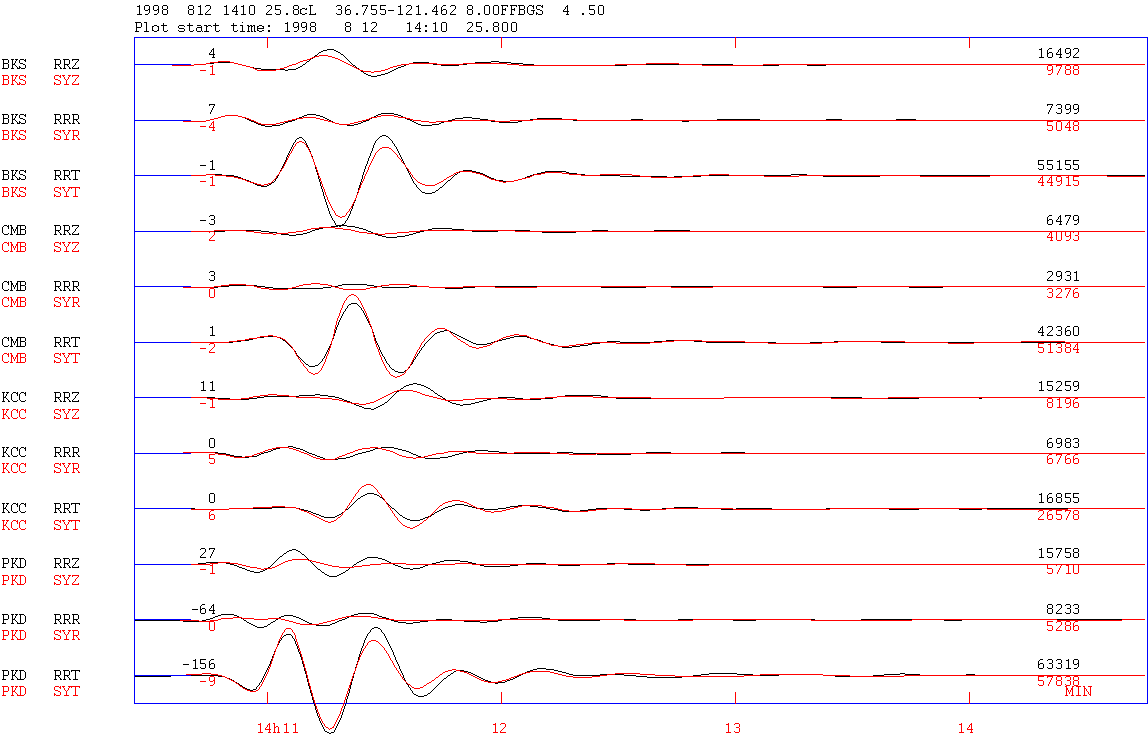
\includegraphics[width=0.9\linewidth]{fig/mt-dreger-1}}
\caption{Plot of original filtered instrument corrected data (blue) compared to the synthetic seismograms (red). The filter used is 0.02 to 0.05 Hz. The plot is made with a fixed scale of 30 000. Note how the T-components dominate the solution. The data is the Dreger test data included in the SEISAN training data. Note that when plotting a file in Helmberger format, the overlay function (see MULPLT section) is turned on automatically for channels starting with SY. }
\label{fig:mt-dreger-1}
\end{figure}

\begin{figure}
\htmlimage{scale=2.0}
\centerline{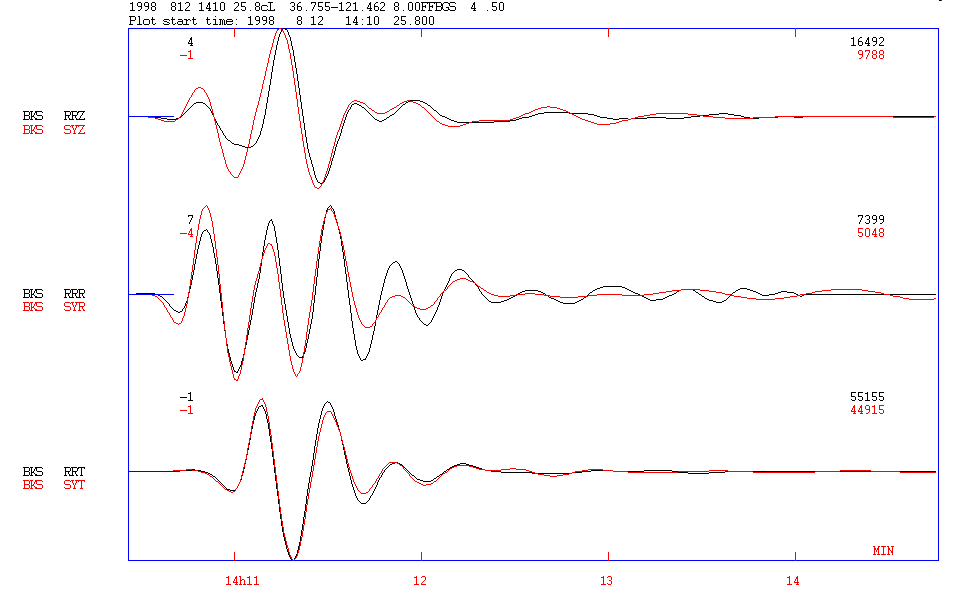
\includegraphics[width=0.9\linewidth]{fig/mt-dreger-2}}
\caption{Same data as shown in previous figure but only for station BKS. The data is now auto scaled. The fit on all channels is quite good. Notice the small amplitude of the radial component.}
\label{fig:mt-dreger-2}
\end{figure}

In the above plots, the original data has been shifted corresponding to the value of Zcor. This means that, for a positive Zcor, the last Zcor data sample on the trace has no data and is replaced by zeros. Similarly if Zcor is negative the first Zcor samples are zero.

\textbf{Judging the results}

See the Dreger documentation for a discussion. Generally the variance reduction VR should be as high as possible.  A bad fit could give an unrealistic moment (and Mw) so that is also an indicator of the quality. 
A good fit is not a guarantee for correct results. If e.g. the gap is large, there might not be sufficiently different data to give a reliable solution, even if the fit is good. The quality given has been assigned by Dreger as follows

\begin{verbatim}
 0 < VR <   20  Quality = 0
20 < VR <   40  Quality = 1
40 < VR <   60  Quality = 2
60 < VR <   80  Quality = 3
80 < VR <  100  Quality = 4
\end{verbatim}

It is necessary to check the solution against the P polarities to confirm that they generally match the solution as wrong alignment can result in inverted solutions. However, it is not to be expected that all the synthetic polarities fit the observed polarities since the fault plane solution from MT (measures overall slip) might be different from fault plane solution with polarities (measures the slip of the initial rupture). Use command fo to plot the solution together with observed polarities recorded in the S-file. 

\textbf{Example of a run of the inversion}



\begin{verbatim}
#    2 12 Aug 1998 14:10 25  L  36.755-121.462 8.00FF  .50     BGS    4  ? mti

***Event to invert***: C:\Seismo\\REA\TEST_\1998\08\12-1410-00L.S199808

Inversion in:             displacement
Number of stations:              4
Number of points to use:       250
Depth:                         8.0
Sample rate:                 1.000
Reduction velocity:            8.0
Filter:                      0.020   0.050

Skip for down sampling for PKD    20
Skip for down sampling for BKS    20
Skip for down sampling for CMB    20
Skip for down sampling for KCC    20

PKD   Distance(km)=   122.0 ShiftVel(s)=     0.1  Offset(sample)=    0
BKS   Distance(km)=   142.0 ShiftVel(s)=     2.5  Offset(sample)=    0
CMB   Distance(km)=   171.0 ShiftVel(s)=     6.2  Offset(sample)=    0
KCC   Distance(km)=   201.0 ShiftVel(s)=     9.9  Offset(sample)=    0

Writing PKD__.green            ShiftVel: Shift in s due to reduction velocity             
Writing BKS__.green            Offset:  Zcor parameter in S-file
Writing CMB__.green
Writing KCC__.green

Output from tdmt_invc:         See Dreger manual for following output

Depth=8
Station Information
Station(0): PKD__.data  R=122.0km  AZI=137.0  W=1.000  Zcor=14
Station(1): BKS__.data  R=142.0km  AZI=331.0  W=1.164  Zcor=13
Station(2): CMB__.data  R=171.0km  AZI=34.0  W=1.402  Zcor=13
Station(3): KCC__.data  R=201.0km  AZI=71.0  W=1.648  Zcor=12
Mo=4.12984e+023
Mw=5.0
Strike=223 ; 130
Rake=18 ; 172
Dip=83; 72
Pdc=98
Pclvd=2
Piso=0
Station(0)=78.607796  4.95437e+010
Station(1)=82.944862  3.37622e+010
Station(2)=82.605667  1.91152e+010
Station(3)=56.903259  6.36377e+009
VAR=7.48972e+006
VR=79.39  (UNWEIGHTED)
VR=79.00  (WEIGHTED)
Var/Pdc=7.668e+004
Quality=3

Update event with new mt solution(n=enter/y) ?
\end{verbatim}

\textbf{How and where parameters are changed for making tests}

After the first parameter file in the S-file has been made, these parameters can only be changed by manually editing the S-file or deleting part or all of the parameters in the S-file and running command \texttt{mtp} again. Possible changes:

\begin{itemize}
\item 
New model: Delete in S-file, edit station file and run \texttt{mtp}. Or correct directly in S-file. However if a new model results in new distances and azimuths, then the station lines should also be  deleted before using \texttt{mtp}. Similarly with the depth line if depth changes.
\item 
New depth: If location is unchanged, only change depth in parameter file and start with step 3.
\item 
Range of depths: Edit S-file depth line.
\item 
New event location: Delete station lines in sfile and start with step 2.
\item 
Take out some stations: Change the ID in the first station line (the one with mt specific parameters), e.g. write xSTATION instead of STATION. Then run inversion again, step 5.
\item 
Take out components for a station: Edit the field \texttt{MT-COMP: TRZ}, see below. Then run inversion again, step 5.
\item 
Change filter: A new data selection in MULPLT must be made with the new filter and the new filter must be written into the S-file. There is a check if filter in S-file corresponds to filter in data file. Then continue with inversion, step 5.
\item 
Add a completely new station: Start from the beginning, this requires complete data selection and computation of Green's functions. The simplest is to delete all parameters with mtd.
\item 
Change from displacement to velocity: Start from the beginning.
\item 
Change sample rate: Change in S-file and start from step 3 making Greens functions. Remember to change the number of points for inversion correspondingly, that is e.g., if sample rate is doubled, number of points must also be doubled to analyze the same length time window.
\item 
Change reduction velocity. Change in S-file and ideally start from step 3. However, starting from step 4 gives the same result provided the time window is long enough, see also below.
\item 
Adjust  time shifts:  Zcor gives the number of samples the data automatically has been shifted to correlate with the Greens function. Check how the synthetic seismograms fit the observed seismograms. This number can be adjusted in the s-file. The number should be Zcor plus or minus a few data points. If zero, the automatic correlation is used. \textit{If real data is seen to the left of the synthetics, reduce Zcor and increase if the data is to the right of the synthetics} (indicated on top of plot as \"Data left. -Zxor\"). Zcor can be positive or negative.
\item 
In general, if deleting a line with parameters, they can be regenerated by command mtp.
\end{itemize}

If a range of depths is used or the new mt solution is updated, the mt is written to 
a file named \texttt{psmeca.in} that can be used to plot the mt solution with 
the GMT program \texttt{psmeca}. With the command\newline
\texttt{psmeca psmeca.in -R10/80/0/42 -JX16/-20 -Sd0.3 -Gred -P -B10f5:"Variance reduction":/1:Depth: $>$ mt.ps}\newline
the double couple part was plottes in figure \ref{fig:mt-depth}. 
Using \texttt{-Sm0.3} will show the mt.

\textbf{Summary of mt related commands in EEV}

\begin{itemize}
\item 
mtp	Make parameters
\item 
mtd	Delete all parameters
\item 
mtg	Make Greens functions
\item 
mti	Make inversion
\item 
pm	Plot observed and synthetics
\item 
pd	Plot mulplt.wav
\item 
pg	Plot greens functions
\item 
fo	Plot fault plane solutions
\end{itemize}

\textbf{Influence of parameters}

\textit{Filters}: Try to find a filter giving a good signal to noise ratio. There can be substantially difference using different filters. 

\textit{Reduction velocity}: It has little influence on the results except that Zcor changes due to relative change in arrival times. It is normally selected to include signals before the P arrival and to include all surface waves. Even different reduction velocity for real and Greens function data does not matter. The use of reduction velocity only has the purpose of reducing the length of the traces by putting events close in time. This is particularly important when using events in with a wide distance range.

\textit{Time window}: The most important is that the time window includes the whole time signal to be inverted. The time window actually used by the program will depend on how close it is to a $2^n$ number. \newline
The correlation is done only with $2^n$ samples. The number of samples selected for correlation can be both larger and smaller than the number of samples in the data file. E.g. if number of samples is between 90 and 181, 128 samples will be used and if between 182 and 362, 256 samples is used etc.\newline
The inversion also seems to use a $2^n$ number and there can, in a few cases, be a radical difference between using e.g. 256 and 257 points in calculating the fit VR, but apparently not the solution itself. The default number of samples to use is therefore 257.   So if the number of samples is near a $2^n$ number, use a number a bit larger than $2^n$. This change in fit is not generally observed, in most cases VR is not affected.\newline
Inspect the Greens function file all.green (command pd) or use MULPLT with all.green\$\$\$ to see how long the Green function signal is and similarly look at the data files. The time shifted data files are STAT.data and can be plotted with MULPLT.

\textit{Sample rate}: Seems to have little influence if well above the frequencies of analyzed data. One or two Hz seems ok for data where the inversion is made for frequencies below 0.1 Hz. For 1 Hz data 4$-$8 Hz or similar (depending on sample rate of original data).

\textit{Number of stations and components}: It is often difficult to get good results with all stations and components. Start with a few stations (even one god one) and gradually add data. Note that changing station configuration also can change the time shift between synthetic seismograms and the data. It is important to have as small a location gap as possible.

\textit{Zcor}: Zcor is calculated by correlating the Greens functions with the data and the synthetic seismograms might need a correction as observed from the overlay seismograms. The Zcor time shift will change with different solutions so there is no final Zcor that will work in all cases. Small changes in Zcor can significantly improve the results. In the worst case, Zcor might have to be large enough to reverse the polarity of a signal or even larger if e.g. P has been correlated with S (small events at higher frequencies). The automatic correlation is what creates most problems. 

\textbf{What can go wrong}

\begin{itemize}
\item 
Very bad fit. This can be caused by the correlation not working well, Signals might be shifted several cycles. Try using a different time window, particularly a longer one.
This can also be cause by a bug which results in a factor 2 wrong sample rate. it is clearly seen whan comparing the synthetics and real data. Just run again usually fixes the problem:
\item 
Crash of inversion program. This might be caused by correlation not working. Zcor for a particular station might have  a value of millions. Do not use the particular station.
\item 
Deselecting components does not always seem to work, then use all 3 component or deselect station.
\item 
The invasion does not start. Use \texttt{Ctrl+c} and start again. 

\end{itemize}

\textbf{Rerunning a previously analyzed event}

The S-filer contains all a parameters used including the start time and duration of the data file so it is possible to extract the same data file for the same channels again. The Green's functions must be regenerated by command mtg. If the user does not delete the backup files (see above) the data file is available as backup file and a question will be given if the previous data file should be used.


\textbf{Running the programs independently of EEV}

Once a first run has been made, the programs can be run independently of EEV using the original parameter files. This can be an advantage if the user wants to change some of the hardwired parameters. However, this can only be done for one depth.

\texttt{FKRPROG\_SEISAN}: The only parameters which might be tested are the group velocities. Dreger is vague about what they should be but their values seem to have some influence on the Greens function. It is also possible to edit other parameters independently like the model.

\begin{itemize}
\item 
Edit the \texttt{green.par\$\$\$} file (\$\$\$ is depth). 
\item 
Run program \texttt{fkrprog\_seisan}: \texttt{fkrprog\_seisan $<$ green.par\$\$\$}
\item 
Convert to time domain by running \texttt{vwint\_seisan}
\end{itemize}

\texttt{TDMT\_INVC\_SEISAN}: The only parameter that cannot be tested through EEV is to make the analysis window smaller than the data window. This sometime improves the results.

\begin{itemize}
\item 
Edit parameter file \texttt{mt\_inv.in}
\item 
Run \texttt{TDMT\_INVC}: \texttt{tdmt\_invc\_seisan}
\end{itemize}

Running in this way, the synthetic file readable by SEISAN is not generated and cannot be updated with the results.

\textbf{Example of parameters in S-file}

\verbatiminput{include/mt.sfile.example}

Most of the parameters are explained under synthetic seismograms. The new ones used only for mt  and other important ones are:\newline
\texttt{DEPTH--}: The first number is start depth, the following number of depth to test and the last number is the increment in depth. The default is one depth only.
\texttt{MT-NP-USE}: Number of points for the inversion, default 257. The number does not have to be $2^n$ but it seems that, in some cases, a number a bit larger than $2^n$ is better than $2^n$ or a bit smaller.\newline
\texttt{NPOINTS}: Number of points in time domain used to make Greens function, default 512. This number must be $2^n$.\newline
\texttt{MTSTART}: Start time of data window used.
\texttt{MT-WINDOW}: Length (s) of data window used.
\texttt{MT-RATE}: Sample rate to use. This rate will be used for Greens function generation and the observed data will be down-sampled to this rate. \textit{NOTE: The rate must have value so only skipping samples in the data can be done}. So the rate 1 can nearly always be used while rate 3 rarely can be used. The time window for the Greens function will then be NPOINTS/MT-RATE. Default 1.0 samples/s.\newline
\texttt{MT-REDVL}: Reduction velocity, default 8 km/s.\newline
\texttt{MT-FILT}: Filters to use for both data and Greens functions. \newline
\texttt{MTOFFSET}: Offset in samples for the data relative to the Greens function. Default 0.\newline
\texttt{MT\_COMP}: Indicate which component to be used. By default all 3 are used, but any combination can be selected. T, R and Z can come in any order but must be within column 76:78.\newline

\textbf{Technical notes}

The Dreger MT inversion essentially consists of a Green's function generation program, \texttt{fkrprog} (in SEISAN called \texttt{fkrprog\_seisan}), several data manipulation programs and scripts using SAC to prepare data for the inversion program \texttt{tdmt\_invc} (in SEISAN called \texttt{tdmt\_invc\_seisan}).  The two key programs have been left nearly unchanged (all changes are clearly marked in programs) while the data manipulation programs mostly have been replaced by standard SEISAN functions (mostly within EEV) and one modified Dreger program \texttt{wvint9} (now called \texttt{wvint\_seisan}) so only 3 programs have been added to SEISAN. A significant change is that Dreger uses cm as a unit while SEISAN uses nm, so software has been changed to nm like elsewhere in SEISAN. 
The Dreger code has no provision for  using less than 3 channels. However, undocumented information indicates that if a data channel has zeros, it is not used and this is how it is implemented in SEISAN. In some cases it does not seem to work well, should be investigated more.
The data and Greens functions in Dregers software are using the Helmberger format, a simple Ascii format without reference to time and channel name. SEISAN will, for simplicity use the same format, but it has been extended to also include channel information, absolute time and an ID of the event being processed (the S-file name), see example below. 

\verbatiminput{include/mt.helmberger}

The two first lines are main headers. The first line has number of channels in file (format i8) and has been extended with, filter band, number of poles and passes and S-file name. Only the number of channels is required information for plotting. The second line gives format of data, extended with help text which in this case is information that file is in displacement (nm). The following two lines are channel headers for each channel. The first channel header has undocumented information. The second channel header has number of samples in channel (i8), sample interval(s)(f10.3), undocumented and starting from column 32, the station code, channel code and start time.

The program flow in SEISAN is

\begin{itemize}
\item 
Plot, rotate, filter and instrument correct signals. This generates an output file \texttt{mulplt.wav}. A parameter is set in MULPLT to enables the output. This file has not been re-sampled.
\item 
Make parameters in S-file (command \texttt{mtp}): Parameters are selected from \texttt{mulplt.wav} (stations to use, filter and whether displacement or velocity), from s-file (depth, distances and azimuths), from station file (model) and some are hardwired. The operation takes place in EEV. At this point the backup data file is made.
\item 
Generate the 10 Greens functions (command \texttt{mtg}): All old Green's functions are deleted and parameter files to \texttt{fkrprog\_seisan} (\texttt{green.par\$\$\$}, \$\$\$ is depth) are made from the S-file (inside EEV), \texttt{fkrprog\_seisan} is run giving an output file with frequency domain Greens functions \texttt{green.out}. This file is converted to a Greens function time domain files, \texttt{all.green}, with \texttt{wvint\_seisan} (modified version of original program \texttt{wvint9}). Since it is assumed there is no explosive component, only 8 of the 10 greens function are written out in time domain (as the original program). \texttt{all.green} is in Helmberger format. Information of using displacement or velocity is read from S-file. 
\item 
Make inversion (command \texttt{mti}). In EEV, same length time windows, one for each station, are extracted from \texttt{all.green} and \texttt{seisan\_mt.out}. Names are \texttt{STA.green} and \texttt{STA.data}. The old \texttt{STA.green} and sta.data are deleted first. The  Greens function files are antialias filtered with a LP filter of 4 poles at (desired sample rate)/5 Hz (not sure it is needed), re-sampled and time shifted, all in EEV. If a channel has been deselected or not available, zeros are written out. The Greens functions are band-pass filtered and anti alias filtered with same filters as used for the data. The parameter file (\texttt{mt\_inv.in}) for the inversion program \texttt{tdmt\_invc\_seisan} is made (in EEV) and the inversion program started from EEV. The inversion program makes an output file with signals and synthetics (\texttt{synt.out}) which is converted to Helmberger format file \texttt{synt\_seis.out} in EEV. Command \texttt{pm} will plot this directly in EEV. File \texttt{mt\_inv\_redi.out}  (as the original) has details of the results and  is read by EEV to optionally get results back into the S-file.
\end{itemize}

\textit{Fkrprog\_seisan}: The parameter file format has been changed to include station names and the s-file name.\newline
\textit{Tdmt\_invc\_seisan}: The program has minor changes to accept new Helmberger format (it also reads the original format). It did not work properly under Windows with more then 450 points, so memory allocation was doubled to fix this. The plotting routine has been simplified to only write original and synthetic seismograms.

To get correct overlay, the channels must be sorted alphabetically. MULPLT turns on sorting (normally set in MULPLT.DEF) if the filename is synt\_seis.out.
\index{synt\_seis.out} \index{Sorting in MULPLT}

The SEISAN implementation is dimensioned to max 99 stations.

\begin{figure}
\htmlimage{scale=2.0}
\centerline{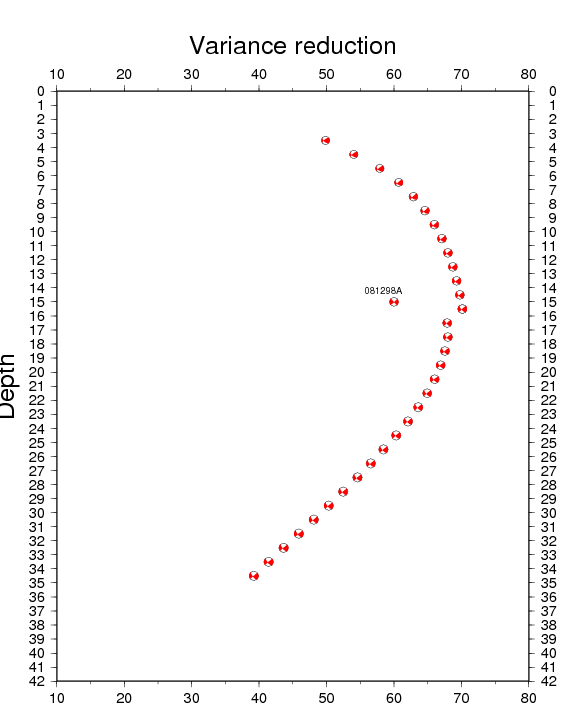
\includegraphics[width=0.9\linewidth]{fig/mt-depth}}
\caption{The double couple part of the moment tensor solution shown with respect to the 
variance reduction at different depths. The GCMT solution is also shown with 
arbitrary variance reduction. This figure was made with the GMT program psmeca, se text.}
\label{fig:mt-depth}
\end{figure}




%
\section{Calculation of coda q, CODAQ}

\index{Quality factor}
\index{CODAQ} 
This section contains the main program CODAQ to calculate coda Q, program CODAQ\_AREA to sort output from CODAQ into areal bins and a help program AVQ to average Q-relations.

Codaq

The program will calculate coda Q (hereafter called Q) for a series of events and stations at given frequencies. On completion, the average values are calculated and a Q vs f curve is fitted to the calculated values. The program will also plot the individual events and filtered coda windows. 

The principle for calculation is the standard coda Q method, whereby a coda window is bandpass filtered, an envelope fitted and the coda Q at the corresponding frequency calculated. The envelope is calculated RMS value of the filtered signal using a 5 cycle window. The program used here is the one described in \citet{havskov1989}. \index{Quality factor, determine with coda}
%�\textcolor{red}{jh-comment: next section rewritten, pelase check...}
The program can only operate in connection with the SEISAN format S-files. The program can use all waveform file types accepted by SEISAN and there can be more than one waveform file in the S-file.  The program will also take advantage of the SEISAN database structure.  

Input: \newline
The calculations are controlled by a parameter file called co\index{Codaq.par}daq.par and the actual event-station combinations to use are given in \index{Codaq.inp}\texttt{codaq.inp}. Example files are in DAT, and with the test data set and the example files in DAT, a test run can be done. An example of a parameter file is shown below: 

\verbatiminput{include/codaq.par}

Start in s-times and Vp/Vs ratio (optinal): Normally the coda window starts at twice the S-travel time from the origin, this factor can be varied and might be chosen differently in special cases. Note that the S-time is calculated from the P-time so a P-time must be present. This also means that if a Pn is used, the coda window will start at 2 times the Sn travel time, which might be substantially different from 2 times the Sg travel time. 
%\textcolor{red}{jh-change: Th
e S-time is calcualted from the P-time using and Vp/Vs = 1.78. 
Optionally, the user can select an Vp/Vs ratio to be used. 
This parmeter is optional so parameter files prior to version 8.3 can be used. 

Absolute start time: If 0.0, above parameter is used. However if different from zero, an absolute start time relative to the origin time is used for the start of the coda window. This might be useful since different start times (meaning different lapse times) might produce different q-values. To use this parameter, one must be certain to choose it long enough which can be checked with the plots. If the absolute start time is smaller than (Start in s-times) multiplied by the s travel time, the station will be skipped and a message given. 

Window length: This is the coda window length in secs. Use at least 20 secs to get stable results. 

Spreading parameter: The geometrical spreading parameter used in q-fit, normally 1.0 is used. 

Constant $v$ in $q = q0*f**v$ : For all $q(f)$ values, $q0$ is calculated using a fixed $v$, use e.g. $1.0$. This parameter has no influence on the individual $q$ calculations. 

Minimum signal to noise ratio: In order to accept a q value for the average, the signal to noise ratio must be above this value. The signal to noise ratio is calculated using the last tRMS ( see next parameters) secs of the filtered coda window and the first tRMS secs of the data file window. If the data file starts with noise or in the P signal, the s/n ratio will be in error. A reasonable value is 5.0. 

Maximum counts to use: If the count value in a coda window is above this value, the window is not used. The intention is to avoid using clipped values. From SEISAN version 7.2, there is also an automatic checking for clipped values in addition to `maximum counts'. 

Noise window in front of signal and length of noise window, tnoise and tRMS: The first number is the number of seconds of noise to plot in front of the signal. In previous versions, 15 secs was hardwired, but sometimes there was not 15 secs of noise before the P. The second number is the length of the noise window used for calculation of the signal to noise ratio. This was earlier hardwired to 5 secs. 

Minimum correlation coefficient: In order to use the q value in the average, the correlation coefficient of the coda q fit must be larger than or equal to this value. NOTE. Correlation values are in reality negative, but are always referred to as positive in the following. An acceptable value depends on the data, try to use a value higher than 0.5 (in reality -0.5) 

Number of frequencies: Number of frequencies to use, maximum 10, 5 is a good number. 

Frequencies and bands: The corresponding center frequencies and frequency 
bands. The frequency band should increase with increasing frequency 
to avoid ringing. E.g. 8,3 means that the signal is filtered between 
6.5 and 9.5 Hz. It is advisable to use constant relative bandwidth 
filtering, to get an equal amount of energy into each band. The relative 
bandwidth is defined as $RBW = ( f_u - f_l )/ f_o$ where $f_u$ and $f_l$ are 
upper and lower frequency limit respectively. Such a filter would 
be e.g. $4\pm1$, $8\pm2$. $16\pm4$. The frequency representing the energy in a 
particular filter band, is the geometric center frequency calculated 
as $f_c = sqrt{f_u f_l }$.
Since the user probably wants to calculate coda Q at the given frequency, the normal 
option (new in SEISAN7.2) is that $f_u$ and $f_l$ are calculated such that the 
given bandwidth (e.g. 4 Hz) is used, but the actual $f_u$ and $f_l$  will 
give the specified central frequency. It is still possible to calculate 
as before, where $f_u$ and $f_l$  will be exactly as specified (but the 
geometrical center frequency will not correspond to specified center 
frequency) by giving the bandwidth as a negative number. 

Default stations: The stations that will be used if not specified in the \texttt{codaq.inp} file. THE LINE MUST CONTAIN AT LEAST SOME BLANK CHARACTERS, if not, stations will not be read from \texttt{codaq.inp} file and the program will crash. Note also that the program will use the first available component in waveform file if no components given in the line following. After reading the parameter file, the program will by default use the \texttt{codaq.inp} file to get the event station information. However, any other name can be used if specified interactively, see below. The station codes can have up to 5 characters. 

The \texttt{codaq.inp} file will consist of a series of lines each giving an event identifier (an INDEX file).  An easy way to generate the file is using the SELECT program. The file can also be generated with EEV using the (C)opy option making a file called indexe\index{Indexeev.out}ev.out. An example is shown below: 

\begin{verbatim}
    1  /top/seismo/seismo/REA/BER__/1992/06/16-0343-38L.S199206
    3  /top/seismo/seismo/REA/BER__/1992/06/16-1311-58L.S199206
    7  /top/seismo/seismo/REA/BER__/1992/06/30-1504-30L.S199206 
\end{verbatim}

The above example only uses the default stations given in \texttt{codaq.par}. Below is an example where particular stations and components have been selected with particular events, for this to work the station line in \texttt{codaq.par} MUST be blank. 

\begin{verbatim}
    1 /top/seismo/seismo/REA/BER__/1992/06/16-0343-38L.S199206
HYA  KMY  BER  ASK  TRO
S  Z S  E B  E S  Z S  Z 
    3 /top/seismo/seismo/REA/BER__/1992/06/16-1311-58L.S199206
HYA 
    7 /top/seismo/seismo/REA/BER__/1992/06/30-1504-30L.S199206
HYA  EGD
S  E  S  Z 
\end{verbatim}

Note that the numbers to the left originate from the index file and do not have any importance. The long name with the directory structure, is the name of the pick file (S-file) in the database, if the S-file is in the local directory, it can have just the event id, in this example starting with 30-....The waveform file name is in the S-file. Following the S-file name is, (like in the parameter file), first a line with station codes followed by a line of component codes. Like in the parameter file, if a component is not given, it will be assumed that the component is S Z. THE COMPONENT LINE MUST BE THERE, EVEN IF BLANK. Since it can be quite a lot of work to generate this file manually with both stations and components, SELECT has an option to generate it, see SELECT. However, SELECT will not give component names so only one componet is used (the first in the waveform file). The file from SELECT is called index.codaq. 
/index{index.codaq}

Below is an example of a \texttt{codaq.inp} file, where it is assumed that the S-files are the current directory. This file can also be generated with DIRF. 

\begin{boxedverbatim}
       16-0343-38L.S199206
HYA  KMY  BER  ASK  TRO 

       16-1311-58L.S199206
HYA
S  E 
       30-1504-30L.S199206
HYA  EGD
S  N S  E 
\end{boxedverbatim}

Program operation: \newline
The program first reads the parameter file, default \texttt{codaq.par} which must be in your current directory. It then reads the \texttt{codaq.inp} file with the events to analyze (also in current directory). The S-file names given here can, as shown in the examples above, be in the database or elsewhere, e.g. in your local directory. In the S-file, the name of the waveform file is given. If more than one waveform file is given, all files will be searched for the specified station and component. The program will first look in the current directory, and then in WAV and thereafter in the WAV database and other directories as given in the \texttt{SEISAN.DEF} file in DAT. The program can therefore work without moving the data from the database, however you can also move both the S- files and waveform files to your local directory. Remember that the S-files must be updated in order to have origin time, since the program uses the origin time and P arrival times from the S-files. 

Running the program: 

\verbatiminput{include/codaq.run}

The program will now start to run. 
%\textcolor{red}{jh-change: 
Alterantively, the progran can be started 
with arguments on the promt line:

\texttt{codaq n parameter-file data-file}

and no questions are asked. n is the choice 0 to 3 above.

If no plot is chosen, one line will appear on the screen for each station used and one for each frequency. The program will start a new page for each new event. If you are plotting on the screen, you will therefore have to hit return to get the next plot. The screen might not have been filled out if there are few data. 

All questions will appear in the text window. At the end, a summary is given, which is the same as logged in the output file \texttt{codaq.out}. 

The abbreviations are: 

\begin{tabular}{lp{10cm}}
H: & Focal depth \\
M: & Magnitude \\
TP: & P travel time \\
TC: & Start time of coda window relative to origin time \\
F: & Frequency \\
Q: & Corresponding coda q, if 0 value is $>$ 10000 or negative \\
S/N: & Signal to noise ratio AV \\
Q: & Average q \\
SD: & Standard deviation for average \\
NT: & Total number of q values at all frequencies \\
N: & Number of q values at given frequency \\
q: & Average of q values \\
1/q: & q is calculated as 1/q  averages, probably the best to use \\
f:1/q: & Q values calculated using the relation derived from the 1/q averages \newline
q = q0*f**v obtained with the average 1/q-values \\
cq0: & Constant q0 obtained using the fixed user selected v \\
v: & Constant v determined \\
%\textcolor{red}{jh-change:} 
cor: & Correlation coefficient on determining q vs f \\
%\textcolor{red}{jh-change:} 
corr: & Average correlation coefficients of individual 
codaq calculations when fitting the envelope, both average and standard deviation is given \\
\end{tabular}

If a station is not present or no P is read, a message will be given. The program will search for the first P arrival time in the S-file. If several are present for the same station, it will use the first. 

Output: 

A file called \texttt{codaq.out} is generated. It contains a copy 
of the parameter file, one line for each event station combination 
accepted by the program (correlation and s/n ratio) and the average 
$q$ values. The $q$ values are averaged directly (indicated by $q$) and $1/q$ 
are averaged (indicated by $1/q$). At the end are the fits to the $q = q0*f**v$ relation. A summary of codaq.out is given in codaq1.out 
%\textcolor{red}{jh-change: 
This relation is calulated using the average Q-values for each frequency and each average is weighted by the number of observations used to calculate the average.  

Output of codaq midpoints, codaq.area

For each accepted Q value, the midpoint between the station and the event together with the corresponding Q and frequency is saved in the file, see example below

2009 1 2 03134 RTCT  -32.25 -67.39    8.0  612.0
2009 1 3 452 6 CFAA  -31.67 -68.16   12.0  881.0
2009 113101828 SALAG -32.63 -68.77   12.0  740.7
2009 118 3 521 RTLL  -31.22 -68.50    1.0  310.1
2009 126185753 AGREL -33.15 -68.95    1.0   61.9

The content is: Event date, station code, lat -lon of midpoint, frequency and Q. This information can be used to plot the areal variation in Q and SEISAN provides one such program, CODAQ\_AREA, see below.

%\textcolor{red}{jh-change:
A file called \texttt{codaq.index} is created. This index file contains all the events accepted for calculating the codaq values and can therefore e.g. be used for making an epicenter map of events actually used (use collect with the index file)  
Output file \texttt{codaq1.out} contains the same output as \texttt{codaq.out} except there is no \texttt{print out} for each event. 

Example of \texttt{codaq.out}: 

\verbatiminput{include/codaq.out}

Above, the one line per q calculations is showing results from different stations. Only the traces selected (fulfilling selection criteria) are shown. The time indicated, is the start time in the waveform file for that particular station. 
In general, the start time for each channel of digital data would be different. If some data is missing, it is also show in the \texttt{codaq.out} file. Corr is the average correlation coefficient (with standard deviation) for the data selected for that frequency. The average lapse time is the average of the tc - values. 

In the DAT directory, there is an example \texttt{codaq.par} and \texttt{codaq.inp} set up to run on PC assuming that SEISAN has been installed under \\seismo. If installed differently, edit the \texttt{codaq.inp} file to reflect the installation. For Unix testing, the \texttt{codaq.inp} MUST be edited to reflect the installation path or the file is regenerated using EEV as described above. 

General recommendations: Coda window should be 15-25 seconds, minimum correlation coefficient larger than 0.5. For comparing coda values in different regions, ALL processing parameters must be identical and average lapse times should be very similar. 

Figure \ref{fig:codaQ} gives an example of a codaq plot. There are 
no options for the codaq plots and the length of the window is always 
the first 200 secs from the original trace. If origin time or coda 
window is outside this 200-sec window and data is available, the 
program continues, but the coda window is not plotted on the figure. 

\begin{figure}
\htmlimage{scale=2.0}
\centerline{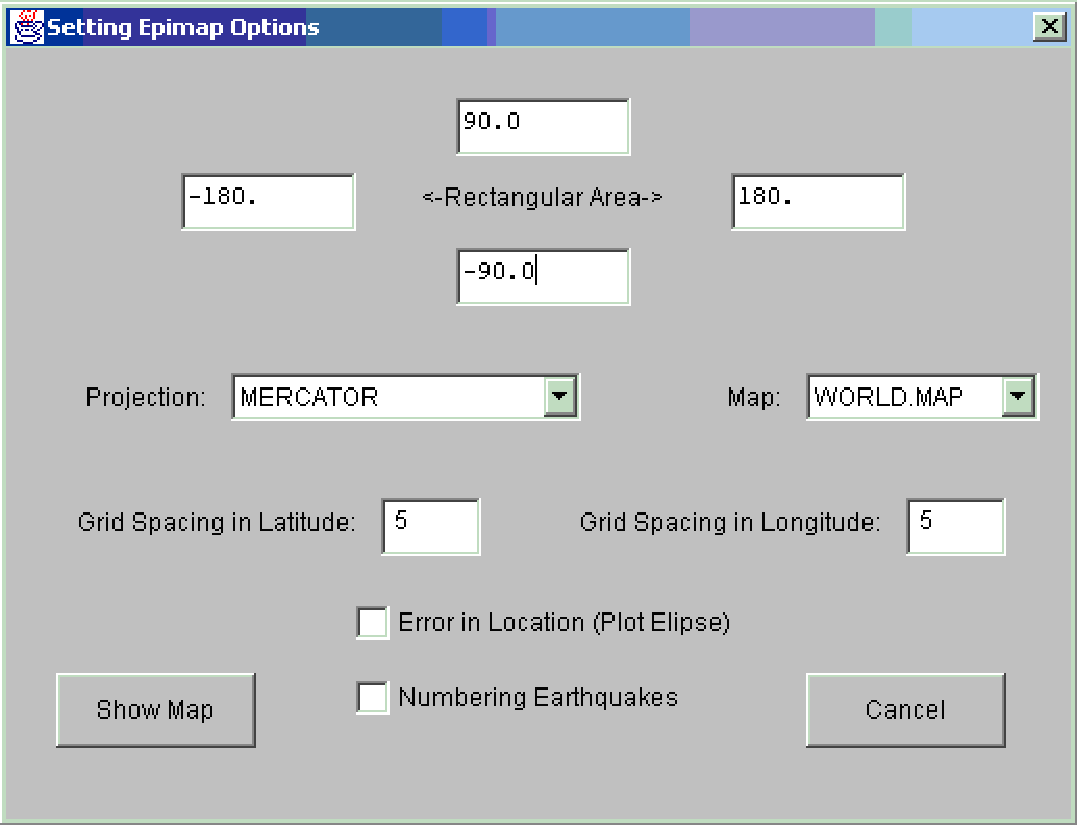
\includegraphics[width=0.9\linewidth]{fig2/fig8}}
\caption{
An example of a coda Q plot. On top is shown the original 
trace and below the filtered coda windows. Note that 15 secs of noise 
are shown in front of the selected filtered coda window. The first 
5 secs of the noise shown is used for calculating the S/N ratio. 
On each filtered plot is given F: Center frequency, Q: Q-value, zero 
means no Q-value could be calculated, S/N: Signal to noise ratio. 
}
\label{fig:codaQ}
\end{figure}


Program CODAQ\_AREA
\index{CODAQ\_AREA}

CODAQ outputs the Q-values at midpoints between station and events. CODAQ\_AREA reads this output and, at each frequency, average Q-values in user defined lat-lon bins. In each bin, provided there is enough data, the Q relation  $q = q0*f**v$  is also calculated. The values in each bin is listed in an output file which can be displayed to get an approximate idea of the areal Q-distribution.

Input files:
It is assumed that codaq.area exists so this name is hardwired. The corresponding codaq1.out is also used to get the frequencies used. 

The interactive options are:

Min no for grid average, min no of freq for Q0 calculation:
Minimum number of Q-values in a bin in order to do an average for that bin, minimum number of frequencies for which Q was calculated in a particular bin in order to calculate Q-relation.

Latitude range and grid size:
Longitude range and grid size: 
Range to use and size of grid in degrees, can be a fraction of a degree.

The interactive options can be stored in a file called codaq\_area.inp. If the file is present, input will be read from that file and no questions asked.

Example run:

\begin{verbatim}
C:\>codaq\_area
Frequencies    1.00    2.00    4.00    8.00   12.00   16.00
 Min no for grid average, min no of freq for Q0 calculation
3 4
 Lattitude range and grid size
-34 -28 1
 Longitude range and grid size
-71 -66 1
 Number of q-data in input file        1094
 Number of q-data inside grid           560


 File with areagrid:    codaq_area.out
 File with grid points: codaq_grid.out
\end{verbatim}

Part of areal output file coda\_area.out showing the lat-lon bins, note the midpoint of the bin is used:

\begin{verbatim}
freq=   1.0000000    
       -70.5 -69.5 -68.5 -67.5 -66.5
 -28.5     0     0     0    49    48
 -29.5     0     0    88     0     0
 -30.5     0     0    42     0     0
 -31.5     0     0    61     0     0
 -32.5     0    57    55     0     0
 -33.5     0     0    67     0     0
 freq=   2.0000000    
       -70.5 -69.5 -68.5 -67.5 -66.5
 -28.5     0     0     0   120   117
 -29.5     0     0   115     0     0
 -30.5     0     0   131     0     0
 -31.5     0     0   111     0     0
 -32.5     0   110   145     0     0
 -33.5     0     0     0     0     0
\end{verbatim}

Output file codaq\_grid.out contains details of the averages in each bin see part of file below:


\begin{verbatim}
freq=   1.0000000
   -33.500   -70.500       0.0       0.0         0
   -33.500   -69.500       0.0       0.0         1
   -33.500   -68.500      67.1      20.6         8
   -33.500   -67.500       0.0       0.0         0
   -33.500   -66.500       0.0       0.0         0
\end{verbatim}

The output is: Bin midpoint, average Q, standard deviation in average and number of points in bin.



Program AVQ, average Q-relations

Q as a function of frequency is usually described as

 $q = q0*f**v$ 

If several such relations are to be averaged, it is not just a question of averaging the parameters. In program AVQ, the averaging is done in the following way:

-For each relation, 1/Q is calculated at the frequencies 1, 2, 4, 8 and 16 Hz.
-At each frequency, average 1/Q is calculated using the number of observations in the original determination of Q for a particular relation as weight.
-A new least squares determination of  $v$ in $q0$ is made with the Q-values.

The program uses an input file with q0, v and number of observations, one relation (free format) per line. An example of a run is seen below:

\begin{verbatim}
C:\seismo\WOR>avq
 File name
input.txt
 Q0,alpha,n   100.00000      0.50000000            1000
 Q0,alpha,n   200.00000       1.0000000              10
 Q0,alpha,n   150.00000      0.69999999             500
  Number of curves to average:            3
  Total number of observations        1510
 Q0,alpha,corr   113.20638      0.54150712      0.99998659
\end{verbatim}


/index{AVQ}
/index{Average Q-relations}





\section{Merge events near in time ASSOCI}

\index{Merge events near in time} \index{ASSOCI}

The program will check if two events are close together in time and merge the events if requested. This is partly an alternative to use append in EEV. The program asks for maximum time difference between events to associate. The user will then be asked if events should be physically associated or not. The program is useful when merging a large number of events. The program has two alternatives for merging: 

\begin{enumerate}
\item
Merge events in same data base: One event is compared to the next event in the same data base. If they are close enough in time, the two events are merged and the program moves on to the next event. If 3 events are close in time, only the 2 first are merged. In order to also merge the third, the program has to be run again. 
\item
Merge events from a file into the data base: This option makes it possible to merge from another data base (use SELECT or COLLECT to create a file) without first completely mixing the two. The event from the file will be merged with as many files from the data base as fit the time difference criteria. So e.g. 2 events from the data base can both get the same event from the file included. At the end of the run, two files are output (associ\_rest.out associ\_merg.out) with events which were not merged and merged respectively. These can then be put into another data base with split, if desired. This function can also be used to separate the input file in two files.\index{Associ\_rest.out}

Note: When merging within one data base, the first event will get the next one merged into it. If merging from file into a data base, the event in the data base will always be the first and keep the main header. This thus a safe method when you want to keep the main header uncheged in the data base. 
\end{enumerate}



\section{Making synthetic seismograms}
\label{sect:synt-seismogram}

\index{Synthetic seismograms} 
\index{BOUCH}BOUCH and \index{BOUSEI}BOUSEI, HERRMANN and HERRSEI and WKBJ are all programs which is used for generating synthetic seismograms.\index{WKBJ} 

The full wave modeling programs are written by Bouchon and \index{Herrmann}Herrmann, and for WKBJ, Chapman and Valerie Maupin. Valerie Maupin has integrated WKBJ for SEISAN and written the routines that makes it possible to use specific phases. She has also made many improvements in the original installation of BOUCH and HERRMANN and written a large part of this chapter.   

Bouchon: \newline
The Bouchon program is somewhat modified for SEISAN. The theory, which is quite straight forward, is given in a series of papers (e.g. \citet{bouchon1981}). It is based on a discrete wave number representation of the wave fields. Basically, the source is repeated periodically in space, so that integration over the k-domain is replaced by a series. This implies that the periodicity of the source, L (in km), should be large enough so that the information from fictitious sources does not arrive during the time interval of interest. Roughly r $<$ L/2,  sqrt((L-r)**2+Z**2) $>$ Vp*t where r is the epicentral distance and Vp is the highest P-wave velocity of the model, t is the travel time and Z the hypocentral depth. Only layered (horizontal, parallel) earth model is used. The earthquake source cannot be in the bottom layer or at the surface. 

There are 2 programs, BOUCH and BOUSEI. BOUCH computes the frequency response given the model, the source depth, the focal mechanism, the receiver locations and the orientations of the two horizontal components. BOUSEI takes the output file from BOUCH, multiplies it by the source spectrum and uses an FFT to get the synthetic ground motion (displacement, velocity or acceleration). The user must provide the source function (see below) and the original waveform files must be available in WAV or working directory if a file containing both real and synthetic signal is to be generated. Otherwise, only synthetic data will be seen in the output file. 

Herrmann: \newline
The Herrmann programs HERRMANN and HERSEI \index{HERSEI}work the same way as BOUCHON and BOUSEI respectively. The major difference is that once HERRMANN has been executed, HERSEI can be executed with different fault plane solutions to obtain the time series, while for the Bouchon programs, both programs must be run again. The Herrmann programs are thus faster for testing many different fault plane solutions. 


The description in the following is for the Bouchon programs, but the steps are the same for 
HERRMANN. 

WKBJ:\newline
\index{WKBJ}
As opposed to the seismograms calculated with the Bouchon and Herrmann programs, the WKBJ synthetic seismograms contain only the number of phases selected by the user. The execution time for one run of the program is very short. In addition to making the synthetic seismograms, the program calculates the arrival times of these phases, and write them both on the screen and in the iasp.out file for later plotting (see MULPLT). This is intended to be a tool to help identify phases on the data or on the Herrmann or Bouchon synthetic seismograms: it can by no means replace these two programs, which are much better than WKBJ to model the frequency-dependent character of crustal phases at regional distance. 

WKBJ seismograms have been introduced in seismology by \citet{chapman1978}. More details on the method can be found in \citet{deysarkar1978} and in \citet{chapman1985}. The core of the present program is a code written by \citet{chapman1988} and is part of the seismological software distributed freely by IASPEI. 
The synthetic seismograms are given in displacement. Although their spectra contain low frequencies, one should bear in mind that they represent a high-frequency approximation of the wave field. They include a number of non-physical phases due to truncation of the integrals in slowness p. For the most interesting crustal phases, the epicentral distance is usually much larger than the source depth, and these phases interfere with the physical phases and modify their amplitudes. 

The head waves on an interface appear automatically as a by-product of the reflected phases, as soon as the epicentral distance is larger than critical. That means for example that the Pn phase appears automatically on the synthetic seismogram as a by-product of the PmP phase. In order to synthesize or calculate the arrival time of a Pn or Sn phase, you must then specify 'PmP' or 'SmS' (see below). 

For a receiver at the free surface, the synthetic seismograms must include the free surface reflection coefficient to yield correct amplitude and waveform for the different phases. For S phases, at epicentral distances larger than critical, this includes automatically the SP phase (a P phase which propagates horizontally along the free surface, and which originates from the critical conversion of S to P at the free surface). The critical distance is of the order of the source depth for the Sg phase, and its SP phase usually appears as a large arrival between the P and S wave. The SP phases are physical, but the amplitude of their high frequency part is overestimated with WKBJ. If one wishes to suppress them from the synthetic seismograms, one may optionally do so. With this option, the surface reflection coefficient is omitted and the synthetic seismograms contain only the upgoing wavefield, that is the wavefield one would get in a borehole, after filtering out the downgoing wavefield. Let us note that this option may strongly modify the amplitudes and waveforms of the different phases compared with those at the free surface. 

In addition to the synthetic seismograms, the program calculates the arrival times of the phases you have specified, and write them in the iasp.out file. These times are calculated by interpolation in epicentral distance of the values tabulated in wkbj.tab. For sources close to an interface (in practice for Pg and Sg phases and the source under an interface), there is a limited epicentral distance range in which an arrival time can be calculated. For example, the maximum epicentral distance for Pg is about 250km for a source 0.1 km under Moho in the default SEISAN model. In order to increase the maximal epicentral distance, you may move the source away from the interface, or you may increase the number of ray parameters used in program wkbj\_or.for (parameter 'nnpp') called from wkbj.for. 

All three programs are hardwired to use triangular sources. 

Running the programs 

The programs require input about distances, azimuths, depth, crustal model, fault plane solution, time window, number of points and some modeling parameters. Almost all of these parameters are available within SEISAN. The programs have therefore been modified to use an S-file (Nordic format) as input file with additional information about time window, number of points to model and crustal model. A special format has been used to keep the modeling information separate from other information in the file (see below for an example). The steps to model a particular event are as follows: 

Problem Bouchon: Use fewer layers, ideally just a halfspace under the deepest ray. Th\index{Problem, Bouchon}e programs seems to become unstable if too many layer are used there. 

Step 1 \newline
Edit the event in EEV and mark the stations wanted for modeling with a minuscule s in column 1, ONLY mark the station once. Exit from editor and, within EEV, give the command "synt". This will generate all the necessary default input parameters for modeling, which are stored as comment-lines starting with \index{SYNT}SYNT in the S-file (see below). At the same time, the s's used as markers are removed. Any old modeling information present will remain and override the defaults.However, in case the F-flag is set for the DEPTH parameter, distances and azimuths will be reset according to the current location. 

Step 2 \newline
Edit event again and check if default parameters are ok (see explanation below).  

Step 3 \newline
Run one of the programs BOUCH, HERRMANN or WKBJ. These are known 
commands in EEV.  BOUCH: The program will now run for a certain 
amount of time depending on number of points required. At the standard 
output, the input parameters used will be printed out and for each 
frequency, the number of terms in wave number integration is printed 
out. If the limit of the number of terms is reached, something is 
wrong, try other parameters.
%\textcolor{red}{jh-change: 
The limit is 2. BOUPAR parameter, currently set at default value of 2000. 
The speed of this output (NPOINT/2+1 lines) 
gives a good indication of how long time it will take. \newline
HERRMANN: Takes longer than BOUCH. \newline
WKBJ: Very fast. 

Step 4 \newline
Generate the seismograms. BOUCH: Use program BOUSEI. The program is 
interactively asking the seismogram type (displacement, velocity 
or acceleration). BOUSEI will generate a file bousei.out in SEISAN 
format containing both original and synthetic traces. The number 
of traces is determined by the specifications for each station, 
see below. Output file is \texttt{bousei.out}. \newline
HERRMANN: Use program HERSEI, similar to BOUSEI. Output file is \texttt{hersei.out}. 
\newline
WKBJ: The first command WKBJ also makes the seismograms. Output file is \texttt{wkbjsei.out}. 

In all cases it is possible to shift the original trace relative to the synthetic trace and the program will ask, for each channel, how much it should be shifted. A positive value shifts the real trace up in time (to the left). The default is to shift the trace the amount of the P-travel time residual of the first P found in the S-file for that station in order to line up the P - phases. NOTE: These phases MUST be the same phase types in order to be lined up. If the first modeled phase is Pn and the first observed phase given in the S-file is Pg, there will be a no alignment. The amplitudes for Bouchon are in nm, nm/sec or nm/sec*sec (hopefully !!) assuming a seismic moment of 10 **22 dyne-cm. The output file will normally contain both the original and synthetic traces. However, if no waveform file is available (in local or WAV directory), the output file will contain an empty channel where the original data should have been. The specifications in the \texttt{hyp.out} file determine which traces from the modeled stations are included in the output file. If the specification after STATION is only component (e.g. S), then all 3 channels are shown. If a particular channel is given (e.g. S  N), then only that channel is shown. Only one or 3 channels can be displayed. 
\newline
All output traces are given in Z, N and E or  Z, R and T depending on the parameter file (see below). The channel names are SH, SB and SW for Herrmann, Bouchon and WKBJ respectively. 

Step 5 \newline
Plot the traces with mulplt. This can be done within EEV using the command pw, ph or pb for WKBJ, Herrmann or Bouchon respectively. Since there is no instrument correction, it is a good idea to plot both the modeled and observed signals narrow band pass filtered. E.g. for regional events 0.1-1 Hz and for small local events 2- 5 Hz (depending on sample rate). 

shows an example of the modeling. 

Note: The whole modeling process can be done entirely within EEV and it is intended to be done so. Since the modeling requires updated distances, depths etc when changing model etc, it cannot take its input from the location in the S-file, which only changes when doing an update (see UPDATE program). So when running from within EEV, a location will always be done first to get an updated S-file (in this case the \texttt{hyp.out} file) and this is the reason that the modelling programs use the \texttt{hyp.out} file instead of the S-file for input. This also means that the modeling program can be run separately from any \texttt{hyp.out} file, however it is then up to the user to keep it updated. 

The modeling parameters 

Below is shown an example of part of an S-file prepared for modeling. The file is one of the events in the test data set and by using EEV to find the event, modeling can start immediately. All parameters have been set automatically. 

\verbatiminput{include/s-file.modeling}

MODEL: The model to be used. THICK is layer thickness, VP is Vp velocity, VS is Vs velocity, DENS is density and QP and QS, are P and S q-values respectively. The model, velocities and Q-values are taken from the \texttt{STATION0.HYP} file with first choice from current directory and second choice from DAT directory (like the HYP program). The S-velocities are calculated using the Vp/Vs ratio given there. Moho is indicated with N at the end of the line with the first mantle layer. A Q of zero means 
infinite Q. The densities are approximate values and should be modified. See below for maximum 
number of layers. 

ST-D-RK: Strike dip and rake is taken from an existing fault plane solution for the given event (F-line) if it exists, otherwise arbitrary values are supplied. 
%\textcolor{red}{jh-change: 
(0,0,0) is an explosion.
The convention is Aki and Richards. 

DEPTH: Focal depth is taken from the current solution. The second field can optionally have the letter F (right justified). If this flag is set, the user can give the synt command to update all distances and azimuths used for modeling which will correspond to the latest location determined as e.g. a result of a changed fixed depth or a changed model. The intention with this flag is that the user should be able to set a fixed depth in the S-file header line, give the synt command to update the parameters for modeling corresponding to this depth and then model. 

NPOINTS: Number of points to model, 512 is set as default, must be 2**N. Used by BOUCH and 
HERRMAN only.

TIMES--: Three different times:\newline
TOTAL: The total time window for generating data and synthetic seismograms for all channels, see also REDVELO. \newline
INITIAL:   The initial time of the earliest trace in the output file, with reference to the source origin time. The synthetics at the station with smallest epicentral distance automatically start also at this initial time. \newline
SY-TRACE: The duration of the synthetic seismogram for each channel, might have different start times,  see REDVELO. 

DT-Tsou: Sampling interval (used for WKBJ seismograms only), and half-duration of the source used for all three programs. In all programs, the source is triangular, however BOUCH can optionally use several sources, see below. 

REDVELO: Reduction velocity to calculate the initial times at subsequent distances (put 0. for no reduction velocity).
%\textcolor{red}{jh-change: 
NOTE: Seems to not be correctly implemented so use 0 always.

PHASES-: The names in format A4 (right justified) of the phases to be  synthesized with WKBJ. The phases may be given in any order, with a maximum of  6 phases per line, and there may be several "SYNT: PHASES-" lines. 

Possible phases: 

Pg (direct P from source to receiver) \newline
Sg (direct S) \newline
PmP (includes automatically Pn at distances larger than critical) \newline
pPmP (includes automatically pPn at distances larger than critical) \newline
sPmP (includes automatically sPn at distances larger than critical) \newline
SmS, pSmS, sSmS (includes automatically Sn, pSn, sSn at distances larger than  critical) \newline
SmP, PmS \newline
P1P, P2P, S1S, etc: the same as PmP, SmS etc, but on interface number 1, 2, etc.  \newline
(The free surface gets interface number 0 in the convention taken here.
%\textcolor{red}{jh-change: 
Thus in HYP, PN2 is the same as P1N here. There 
associated head waves are labeled Pn1, Pn2, Sn1, etc. 

COMPON-: RADIAL for radial-transverse components, NORTH for North-South, East-West components. 

STAT-AT: Is "not free" or "NOT FREE" anywhere within column 16 to 25: Optional line. If this option is chosen, the WKBJ synthetic seismograms are calculated omitting the reflection coefficient at the free surface, at the receiver location. 

BOUPAR: Modeling parameters L, Nt and e. L is length of periodicity 
(should be a few times the hypocentral distance), Nt is maximum 
number of terms in wave number summation and e is the value used 
in truncating the summation. Increasing e and decreasing Nt will 
speed up convergence, but the results might be unreliable.
%\textcolor{red}{jh-change: 
If Nt is reached, the results are unreliable.

NEW STAT: Comment line 

STATION: Station to be modeled with component(s) to be displayed. The S means that short period 
instruments are used. 
%\textcolor{red}{jh-change: 
The default is S, so if e.g. BH is used, S must be chaged to BH, else 
the waveform data is not found. If no component is given, all 3 
components are assumed. The other option is to indicate a component (e.g. Z) and only that component will be displayed (see also description of BOUSEI). DISTANC is epicentral distance used, this distance is taken from the current location, AZIMUTH is azimuth from the source to the station taken from current location, BAZIMUTH is the back azimuth at the station, calculated by EEV, used to rotate if so specified. Each new station isrepresented by the above 3 lines. 

\index{Source time function}The source time function 

The time duration of the triangular source time function for Bouchon is given as Tsou above, and is 
also used in WKBJ and Herrmann. 

\index{Hints on modelling}Hints on modeling 

Event 199606071325 in the test data set is set up with modeling parameters and can be tested 
immediately. 

The model 

The standard model given in \texttt{STATION0.HYP} might be too detailed for most cases and should be simplified to include 3-4 layers by just editing the S-file, this also speeds up modeling. However, if you located the event with one model and model with another, the distances and residuals might not fit. A solution could be to have a \texttt{STATION0.HYP} in the local directory with the simplified model. 

Alignment of P and S 

If the distance calculated by HYP is not correct as indicated by P and S residuals, the synthetic and observed signals will not be aligned. The distance for that station can then be changed manually in the S-file under DIST and/or delays can be applied when generating the seismograms. 
%\textcolor{red}{jh-change: 
For line up, it is important that the correct first arrival is included 
in phase list (WKBJ), see what is identified by HYP. If PN2, then P1N must be given for WKBJ.

Testing different parameters 

There is no need to go back to EEV to test for the parameters that do not change the location. Thus to test for different fault plane solutions, time windows, number of points, edit the \texttt{hyp.out} directly and rerun. However, if depth or model is changed, relocation must be made. To test for different depths, locate with fixed depths, see HYP. \newline
NOTE: THE SOURCE AND RECEIVER CANNOT BE AT THE SAME DEPTH (BOUCH AND HERRMANN) AND IN NO CASES CAN THE SOURCE BE AT DEPTH ZERO. 

Running time 

This depends mostly on the number of points and to some degree on number of layers. The number of stations has an insignificant effect on running time.

Program limitations: HERRMANN and WKBJ is set up with max 20 layers and Bouchon with 20 layers. Maximum of 32 stations Change programs and recompile if more layers are needed. Bouchon is compiled for 2048 frequencies (4096) points. 

Computer notes: 

The original Bouchon program BOUCH is almost unchanged. The only modification is that it uses a subroutine to generate its original input file bouch.inp from the \texttt{hyp.out} file. This file still remains after running BOUCH for debugging purposes. The output from BOUCH is \index{Bouch.out}bouch.out, which in turn is input to BOUSEI. 

Herrmann: \newline
The Herrmann waveform modeling is based on a concept where the synthetic seismograms are computed through a sequence of four distinct processes (programs). 

\begin{enumerate}
\item
 The program "hspec8" will calculate the medium response for 10 basic Green's functions, where the response is given in frequency - wavenumber domain F(f,k). 
\item
The program "rhwvinta" will integrate and take the medium response from F(f,k) $\to$ F(f,r) 
\item
The program "rhfoc10" will convolve the response function with a source time function 
and with inverse Fourier transform take F(f,r) $\to$ F(t,r) 
\item
The program "mech" will construct a 3 component synthetic seismogram given a focal mechanism. 
\end{enumerate}


Herrmann's programs originally had several optional source time functions, 
however, a triangular source has been hardwired (for all 3 programs) 
so it is easier to compare the results. The original options can be 
reactivated by editing the program. \newline
The programs HERRMANN and HERSEI run these 4 programs in an automated sequence. 

All References, a detailed manual, source code and parameters as well 
as other related programs: ``Computer Programs in Seismology'', 
Volumes I - VIII. By Robert B. Herrmann, Saint Louis University, Saint Louis, Missouri. 

WKBJ: 

Input file \texttt{hyp.out}, read by "WKBJ. \newline
Output file \texttt{iasp.out}, written by "WKBJ". Contains the arrival times of \newline
the different phases at the stations, in SEISAN format. \newline
Output file \texttt{wkbjsei.out}, written by WKBJ in the SYNTSEL.FOR subroutines. A waveform file (SEISAN type) containing the data and the synthetics, which can be plotted using "mulplt". Note that there is a code for each synthetic seismogram giving the modeling method (SH: Herrmann, SB: Bouchon, SW: WKBJ), and the component (Z, R, T, N or E). 

INTERMEDIATE FILES \newline
\texttt{wkbj.inp}, created by WKBJ for input to WKBJ\_OR. The same information as 
in \texttt{hyp.out}, in a WKBJ\_OR format. \newline
\texttt{wkbj.tab}, output from WKBJ\_OR, reprocessed by WKBJ. 
Contains tables as a function of ray parameter. \newline
\texttt{wkbj.out}, output from WKBJ\_OR, reprocessed by WKBJ. Contains the Green functions. 

\begin{figure}
\htmlimage{scale=2.0}
\centerline{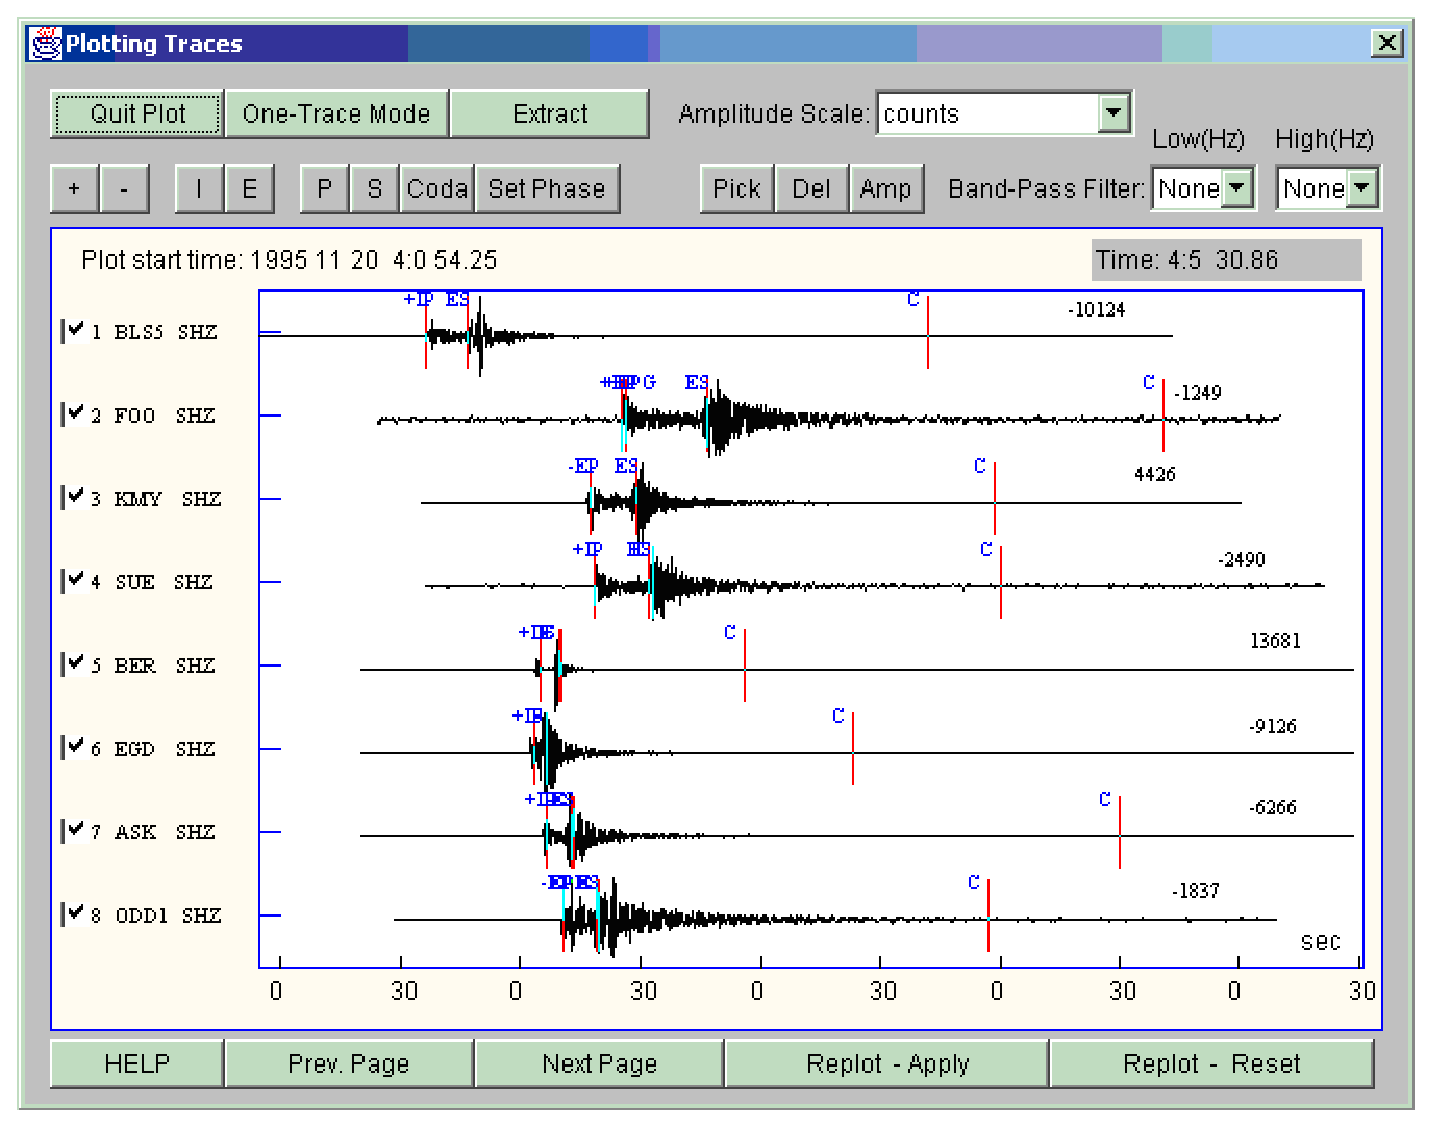
\includegraphics[width=0.9\linewidth]{fig2/fig9}}
\caption{
An example of synthetic seismograms using Bouchon(2),  Herrmann (3) and WKBJ (4). The original seismogram is shown in channel 1. All synthetics are displacement. Also shown are the theoretical travel times calculated by WKBJ. 
}
\label{fig:synthetic}
\end{figure}




\section{Calculation and plotting of travel times} 
\label{sect:cal-plot-tt}

In SEISAN, travel times are generated from a flat crustal model or using the IASP91 global travel time model. It can often be useful to generate travel times for given distances and two programs are supplied to do these calculations. TTIM will calculate travel times for global phases at one given distance and depth and TTLAYER, will calculate a travel time table (layered flat model) for a given depth and a distance range. A special version of TTIM called IASP is used in connection with EEV and MULPLT.  


\subsection{IASPEI travel time software, program TTIM} 

This program can be used for calculating global travel times, see below for details on phases calculated. The program assumes that you have the travel time tables in the working directory or in DAT, see computer notes below on how to generate these file if not already there. The same files are also used by HYPOCENTER. 

After starting the program, the first two questions 'do you want xxxxx' relate to range summaries, etc., that are normally not required and can be answered with n(no) followed by ENTER. The program then asks 'Enter phases, one per line...' You can then enter a specific phase, or a keyword defined as follows:  


\begin{tabular}{lp{10cm}}
All & gives all phases \\
P & gives P-up, P, Pdiff, PKP, and Pkikp \\
P+ & gives P-up, P, Pdiff, PKP, Pkikp, PcP, Pp, Ppdiff, PPKP, 
PPKIKP, Sp, Spdiff, SPKP, and SPKIKP \\
S+ & gives S-up, S, Sdiff, SKS, Ss, Ssdiff, SSKS, Ps, Psdiff, and PSKS \\
basic & gives P+ and S+ as well as ScP, SKP, PKKP, SKKP, PP, and P'P' \\
\end{tabular}

Writing all individual phases, separate by ENTER, terminating the 
list with an additional ENTER.  The program will then enter a loop 
where phase times are calculated for new distances entered on request. 
The program is terminated for a particular distance by entering -1, 
and a new depth can be used, or the program can be terminated by entering -1 again. \newline
A special version of this program used in connection with MULPLT is IASP. \newline
In order to generate the earth model files \index{IASP91.HED}IASP91.HED 
and IASP91.TBL, first run program REMODL, then program SETBRN. The 
program REMODL has the earth model hardwired. Note: These binary files 
CANNOT be moved between platforms. They are included with SEISAN for 
each respective distribution. If lost, they must be regenerated on 
the same platform.  \newline
For more information about IASP91 programs, see HYPOCENTER manual by \textbf{B. Lienert}. 

%\textcolor{red}{pv-change: 
On at \index{64 bit computer} 64 bit 
computer the IASP files must be regenerated 
is you have the files from a 32 bit computer, with the programs \texttt{REMODL} and 
\texttt{SETBRN}. 




\subsection{Calculation of travel times for layer and gradient model, TTLAYER}

The TTLAYER\index{TTLAYER} program is written by Barry Lienert to calculate travel times for both layer and gradient model. In this version the program only works for zero depth, and therefore might not be very useful. The program reads a set of velocities and depths from an input file in `\texttt{STATION0.HYP}' format and calculates travel times for P and S velocities for a set of uniform-velocity layers, using the HYPOCENTER dtdx2 routine and also for a set of uniform gradient layers, using dtdxg, a new routine written to have the same input arguments as dtdx2. \newline
The routine to calculate travel times for a gradient model uses an adapted version of Fred Klein's TTCAL routine, which he uses in his program TTGEN to generate a table of values from which to interpolate travel times and their derivatives in HYPOINVERSE.  \newline
The program is easy to run and the output can be plotted with some standard xy plotting tool. 



\subsection{Plotting of travel times, TTPLOT} 
\label{subs:ttplot}
\index{TTPLOT}

Program to plot observed and calculated travel times (Figure 
\ref{fig:travel-time-plot}
). The input to the program is an s-file, which has an indicator to a model file (\texttt{STATION?.HYP}) and the travel time observations. The program is started by `ttplot $<$sfile-name$>$'. At the start, TTPLOT relocates the event and calculates distances using the HYPOCENTER program. It then plots all observations with a `+' symbol and the theoretical travel times that are calculated by the program for the first P and S arrivals with solid lines. The program can be useful in routine processing to visualize large residuals, which otherwise are seen from the location program output. The program can also be started from EEV using option `ttplot'. It is possible to click on symbols, which will bring up station code, phase, observed travel time and residual on the rigth. The output files are: 

\texttt{ttplot.out} - gives station code, phase name, distance, observed travel times and residual. 
\newline
\texttt{ttplot.eps} -  Postscript version of plot. \index{ttplot.out}\index{ttplot.eps} 

\begin{figure}
\htmlimage{scale=2.0}
\centerline{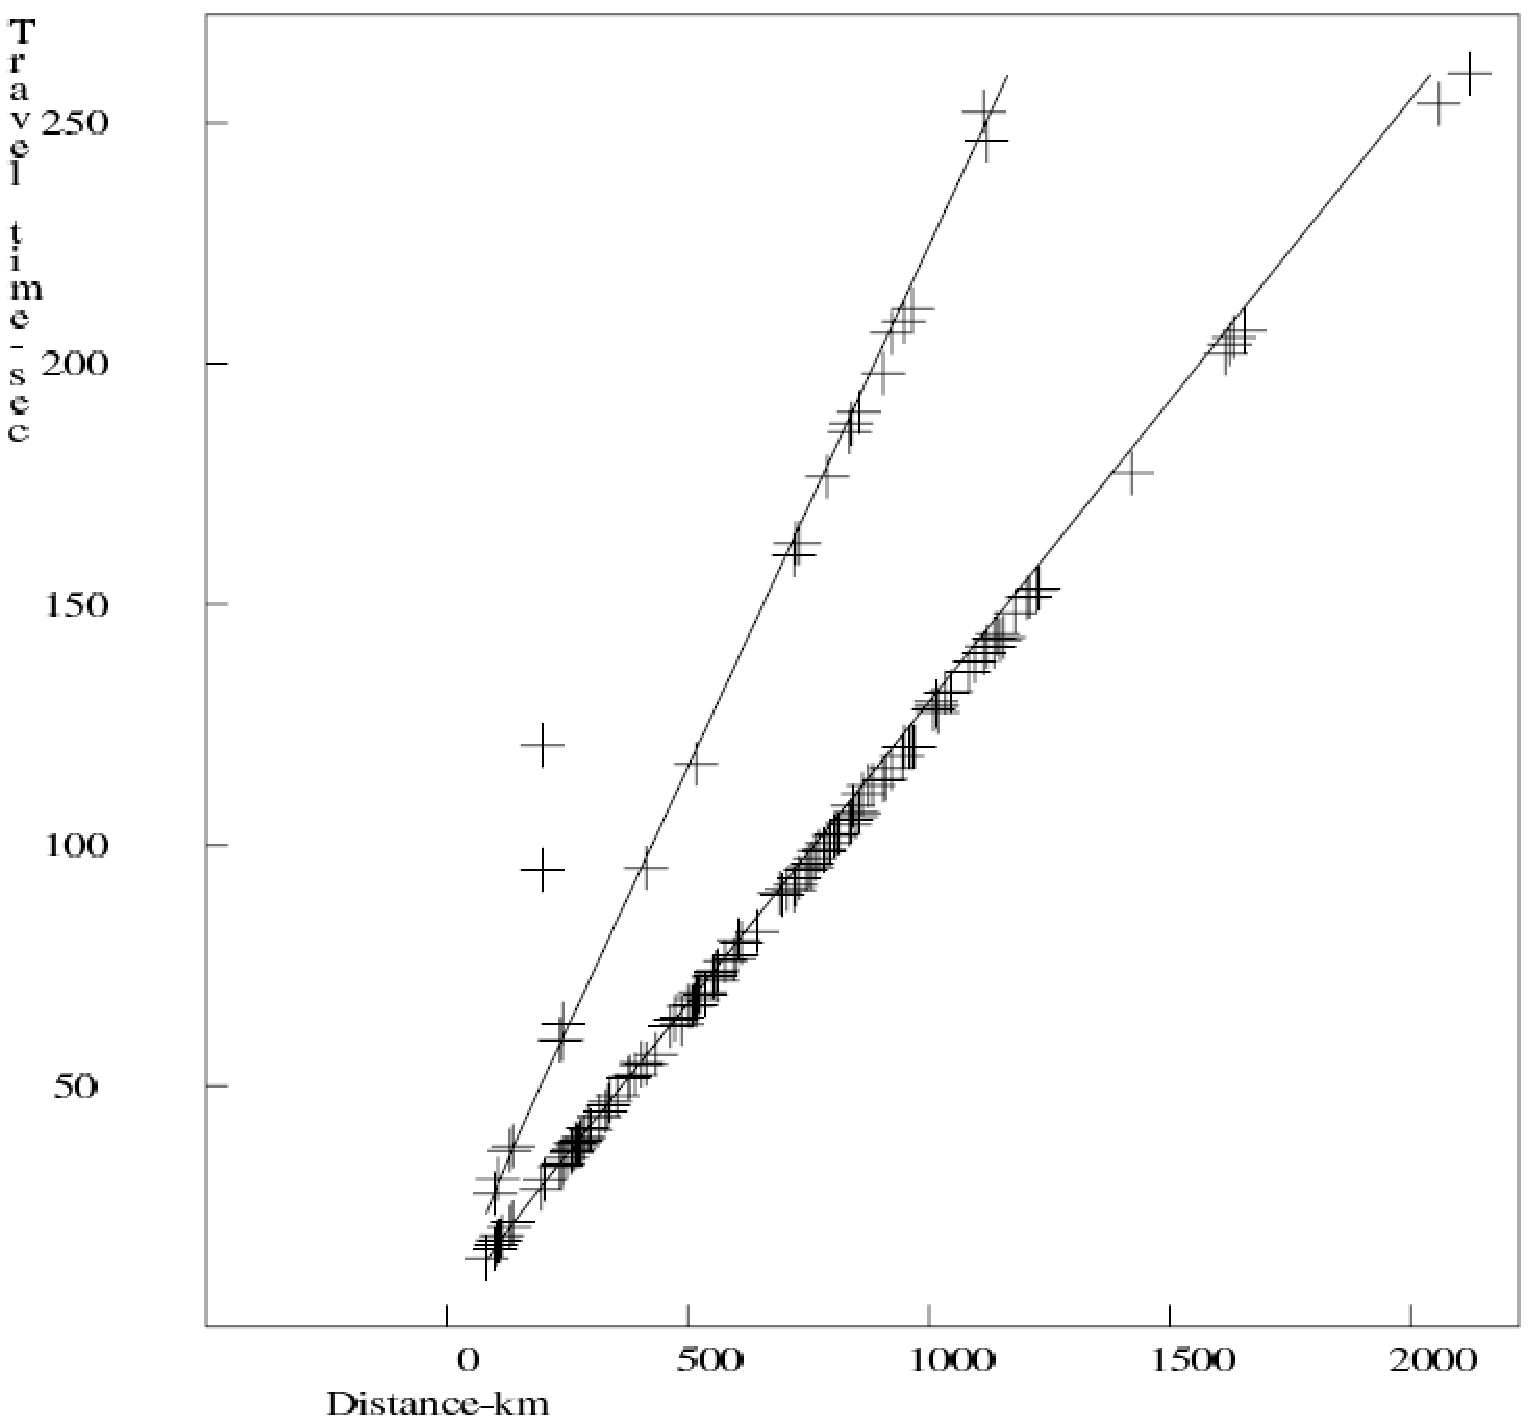
\includegraphics[width=0.9\linewidth]{fig/travel-time-plot}}
\caption{Example of travel time plot. Both P and S observed travel times are plotted with "+"
symbol. Calculated times are shown by the solid lines, the lower one gives the first P arrivals,
the upper line gives first S arrivals. The two outliers are observations from a station with
incorrect timing.
}
\label{fig:travel-time-plot}
\end{figure}




\subsection{IASP, travel times for MULPLT} 
\label{subs:iasp}

This program is a special version of IASP91 to be used in connection with EEV and MULPLT. Giving command iasp from the EEV prompt (or from within MULPLT), the program will read the current active S-file, and for each station, calculate possible IASP91 phases and arrival times relative to the hypocenter and origin time given in S-file. The origin information can be obtained from two places in the S-file: (1) The header lines are searched for hypocenter lines and the first found after the main header will be used, (2) If no secondary header lines, the main header line is used. The intention of this order is that it is possible to put in a PDE solution in a secondary header line (option INPUTONE in EEV) so that theoretical travel times are calculated relative to a fixed solution and not the temporary solution made by the local agency. 

The IASP91 tables can be found in the local directory or DAT and have the same names as used in HYP and TTIM. The program generates an output file iasp.out in Nordic format. This file is read by MULPLT and the theoretical phases displayed on the screen. The number of phases calculated can be very large making it hard to see which phase is which. IASP therefore has a definition file, IASP.DEF, where phases to be written out are given. The file can be in the working directory \index{Iasp.out}\index{IASP}or in DAT. If no definition file is available, all phases will be written to the iasp.out file. Below is an example of a IASP.DEF file. 

\verbatiminput{include/iasp.def}



\section{Inversion for $Q_{Lg}$, QLG} 

The QLG program can be used to determine an average $Q_{Lg}$ or to 
perform a tomographic inversion. The method is described in \citet{ottemoller2002}. 
Here, we use the same names for the damping parameters, and many of 
the other parameters should be self-explanatory. The program can also 
produce the input for distance trace plots. Note that using the program 
is no trivial task. The data set needs to be carefully selected and 
the instrument calibration has to be known. The input to the program 
is a Nordic file, which includes several events. The parameter file 
needs to be carefully set up.\index{Lg waves}\index{$Q_{Lg}$} 

The program can be used in the following way: 
\begin{enumerate}
\item
Determine average $Q_{Lg}$ 
\item
Perform checker-board test to chose damping parameters 
\item
Tomographic inversion 
\end{enumerate}

Note: The main purpose of including the program is to give an example source code so that the user can make use of it when implementing similar programs. The program uses a linear grid... 

Example of the parameter file \texttt{qlg.par} : 

\verbatiminput{include/qlg.par}

\citet{menke2006} pointed out the non-uniqueness in attenuation tomography between the source term and Q. They suggest to investigate the non-uniqueness by synthetic tests in which a perturbation is applied to the source term and the inversion for Q is done without inverting for differences in the source term. The solutions obtained are null-solutions and one needs to be careful not to mistake them for real patterns. These tests are possible within QLG by setting the parameter `SOURCE PERTURBATION, where the first parameter refers to the source that is perturbed and the second parameter gives the amount of perturbation in units of moment magnitude. 

It is possible to invert real data without inverting for the site term by setting `FIX SITE'. This can be a useful test as there is also a trade-off with the site term. Fixing the site term is more problematic, as this is done based on the local magnitude, which may not be the same as the moment magnitude. 

Another useful stability test is to add Gaussian noise to the spectra and check the inversion result. This can be done for both real data and the checkerboard test by setting the parameter `GAUSSIAN NOISE', units are equivalent to change in moment magnitude. 



\section{Wadati} 

This is a program to make Wadati \index{WADATI}\index{Apparent velocity}\index{Vp/Vs, calculate}diagrams and apparent velocity from a Nordic file with one or many events. The apparent velocity is calculated from the arrival times and the calculated epicentral distances as given in the S-file. The apparent velocity is thus approximate and affected by the location. \newline
The purpose of the program is to calculate Vp/Vs values for individual events and calculate the average for a group of events. In addition, the program can calculate the apparent velocity for each event based on P or S-times. Wadati diagrams with plot can also be calculated directly from EEV. 

The information can be used to obtain a first impression of crustal \index{Crustal parameters}parameters. 
For each calculation, events can be selected based on: Minimum number of stations, maximum rms of the fit (S-P vs P, or arrival times), and minimum correlation coefficient of the fit. For the apparent velocity calculation, the data can also be selected in distance and azimuth ranges. 

The output gives: 

\begin{tabular}{lp{10cm}}
T0 : & Wadati calculated origin time \\
N : & Number of stations used for Vp/Vs \\
VPS : & Vp/Vs ratio \\
NP : & Number of stations for P- velocity \\
NS : & Number of stations for S-velocity \\
AVSP: & Average S-P times with sd \\
AVDI: & Average distance with sd \\
\end{tabular}

The average Vp/Vs is calculated for the whole data set. Individual Vp/Vs values outside the range 
1.53 to 1.93 are excluded. An output file wadati.out is generated. A minimum of 3 stations is required for an event to be used. Only same type phases are used (like PG and SG).  

Example of a run to calculate Vp/Vs 

\verbatiminput{include/wadati.run1}

Example of a run to calculate apparent velocity

\verbatiminput{include/wadati.run2}



\section{Calculating spectra, the SPEC program}
\label{sect:spec}
\index{SPEC}
\index{Spectral analysis} 

The SPEC program is used for making spectra of many seismic signals 
in a semiautomatic manner. It can be used for several investigations: 

A: Making a large series of signal spectra, which can be corrected for instrument and path.  

Average spectra are calculated. There are two options for further processing the calculated spectra:  \newline
Option (1): Calculate acceleration density spectra which are plotted compared to the Peterson noise model.\index{Peterson noise model}\newline
Option(2): Using the slope of the flat part of the displacement spectra to calculate the near surface attenuation kappa (see \ref{subs:spec}.  \index{Kappa, determine}

B: Making relative spectra of seismic events or background noise in order to determine the soil response. When using relative spectra of horizontal versus vertical components, this is referred to as the Nakamura\index{Nakamura}\index{Soil amplification}\index{Spectral parameters}\index{Spectral ratio}\index{Quality factor, correct for}\index{Quality factor, determine by spectra} method \citep{nakamura1989}. 

C: Making relative spectra of signals from two stations in order to determine Q. The program makes output files for generating GMT plots in addition to standard SEISAN plots. 

Note: Parameter file has changed between SEISAN 7.2 and 8.0 (number of windows and overlap has been added). \newline
The program can technically operate in two ways: (1) Making relative spectra of a series of pairs of stations terminated by the average spectra, (2) Making a series of spectra for a number of stations and events. The spectra can be corrected for distance, Q, and instrument response. In addition, the spectral levels can be expressed in m\index{Moment}oment or moment magnitude calculated in the same way and with the same units as in MULPLT. All relevant parameters are taken from the CAT files, the CAL files and the input parameter file for SPEC. Window selection for the spectra can be specified to be related to the P, S arrival times or the earthquake origin time and it is thus possible to automatically make e.g. S-wave spectra of a large set of stations and events. Op\index{Noise spectrum}tionally, noise spectra, can be calculated together with the signal spectra. The noise window is selected at the start of the waveform file. \newline
Before the program is started up, the input files must be prepared. The program need two input files. The parameter file (default spec.par) gives the parameters to use and the list of stations to process. The event file (default spec.inp) is a CAT file with events to use or a \texttt{filenr.lis} type file with waveform file names (can only be used if no readings are needed, like for Nakamura studies). An example of a spec.par and spec.inp file is found in DAT. These files can be used immediately with the test data set. 

The program produces several output files. The main output is in \texttt{spec.out} with the parameters used, the station event combinations used and error messages. The other files are giving output of most graphs shown. These ASCII output files can be used in other plotting programs, however they have been specifically formatted for the SEISAN GMTXY plotting script. Note that the numerical values given for the spectral output given in those files is the same that appear on the plots and the values are linear. So if a spctrum has been instrument corrected and smoothed, that is what is given. Similarly if a relative spectrum is used.  The number of files depends on number of stations used. Examples of files could be 

\begin{tabular}{lp{10cm}}
\texttt{spec\_all\_ASK\_\_S\_\_Z.out} & All spectra from ASK, S  Z \\
\texttt{spec\_all\_BER\_\_S\_\_Z.out} & All spectra from BER, S  Z \\
\texttt{spec\_all\_gmt.out} &   All spectra from ASK and BER \\
\texttt{spec\_ave\_ASK\_\_S\_\_Z.out} & Average spectrum from ASK, S  Z \\
\texttt{spec\_ave\_BER\_\_S\_\_Z.out} & Average spectrum from BER, Z  Z\\
\end{tabular}

In order to plot these files with GMTXY (only Unix), give e.g. command

\texttt{gmtxy spec\_all\_ASK\_\_S\_\_Z.out}
\newline
There is one more output file, spec\_amp.out, which gives the log log spectra of  of all traces calculated (possibly instrument corrected) before smoothing takes place.
\index{spec\_amp.out}
\index{Spectral output file}
\newline
Limitations of amount of data: The program is set up to handle 300 spectra of up to 30000 points each for one run. The dimensions can be increased in spec.for, however the program must then be recompiled. The spectral windows are 10\% tapered. The analyzed signals will be checked for clipping and rejected if clipped. A message is then given in spec.out 

\index{Spec.par}
The \texttt{spec.par} file The file contains alternate lines of parameter names and parameter values, and must contain the number of lines shown in the example below. 

\verbatiminput{include/spec.par}

The parameters: \newline
\textbf{Selection criteria}: Determines how the start of the time window is selected. 1: Start with the P-arrival time, 2: Start with the S-arrival time, 3: Start with the S-arrival time calculated from the P-arrival time assuming a P to S velocity ratio of 1.78, 4: Start with 'start' (see next parameter) seconds after the origin time as given in the CAT file header. This option can be used if no readings are available in the CAT file. When using a P or S-time for start of window, the program uses the first P or S phase found in the CAT file for a given station. Component is of no importance here, so there is only a need for 
e.g. one P-time for the station being processed if 3 component data is used. This is also the case when rotating the signal, see below. However, on the trace plots, only readings on those components shown will be seen on the plots. 

\textbf{Start}: If the selection criterion is 1,2 or 3, this is the number of P or S travel times (from the origin) used to find start time of window. Use 1.0 if the window shall start exactly at the phase time picked. If selection criteria is 4, start is the number of seconds after the origin time. 

\textbf{Window length, \#of windows, overlap}: 

\begin{itemize}
\item[-]
Window length: Window length in secs for both signal and noise (if selected) . 
\item[-]
\# of windows: If more than 1, spectra will be made in several windows following the first window 
and average spectra will be made. This option can only be used if selection criteria is 4. Used for 
noise studies or Nakamura studies. 
\item[-]
Overlap: Windows can overlap (factor $<$ 1.0) exactly follow each other (factor=1.0) or have gaps 
(factor $>$ 1.0). E.g. 0.9 is equal to 10 \% overlap. 
\end{itemize}

\textbf{Number of times to smooth}: Number of times to smooth, 0 means no smoothing. 

\textbf{Gain factor of channel 1}: Factor that the spectral level for channel 1 is multiplied with. This can be used if the response shape is the same for the two channels and only the levels are different. If the shape is also different, set factor to 1 and use response removal \index{Response removal}below. 

\index{Noise spectrum}
\textbf{Noise spectrum}: If 0, no noise spectrum, if 1, make noise spectrum. The noise window is taken from the beginning of the trace and the window length is the same as given above. 

\textbf{Make relative spectra}: If zero, no \index{Relative spectra}relative spectra, if 1, make relative spectra. The relative spectra will appear one on each page, and the average relative spectrum on the last plot (see Figure 
\ref{fig:spec-example}
). If no relative spectra are chosen, only one trace and one spectrum is shown per page and the average spectrum is shown on the final plot. MUST BE SET to 1 to calculate Q, see below. 

\textbf{Plot pics}: If 1, the phase pics in the CAT file spec.inp will be plotted. 

\textbf{Frequency band used}: Lower and upper frequency bands for the spectral plots. 

\textbf{Response removal}: If 0, no response is removed, else 1: displacement, 2: velocity, 3: acceleration (units is nm, nm/s and nm/s*s), 4: Power spectral density in dB relative to ((1m/s**2)**2)/Hz. This option is used for seismic background noise studies.\index{Power spectral density}\index{Background noise}\index{Noise study}, 5: Determine kappa. The flat part of the spectrum (frequency below corner frequency) is approximated by a straight line and kappa calculated for each event and the average at the end (in spec.out file and on final plot). The spectrum will normally be corrected for Q, BUT NOT kappa. For more details, see \citep{havskov2010}. Make sure to set appropriate frequency limits and correct distance corrections. Can be used for both P and S-spectra. A cal file for each channel must be available in the CAL directory (see section 4.6). For relative spectra, the response removal has no importance if the response is the same for the channels compared. A simple correction can be made with "Gain factor of channel 1" parameter above. NOTE: If moment or magnitude spectrum is made, response removal MUST be 1. 

\textbf{Rotate components}: If 1, the horizontal components are rotated. This means that if the user has specified N or E, radial or transverse respectively will be used instead. The original data remain unchanged. If start time of spectra are chosen by using P or S, there must be a reading from those components if the pics are to be plotted. If the parameter is zero, no rotation is done. See also MULPLT for more details of rotation. 

\textbf{Q0, qalpha and kappa:}

Q-correction: \newline
Parameters in Q-relation Q = Q0**qalpha used for spectral correction (see also section on MULPLT for standard attenuation relations). Only used if response is removed. If first 2 parameters are 0,0, no Q-correction. New from SEISAN7.2 is that a kappa correction also can be used (see MULPLT spectral section). 

Calculation of Q: \newline
If Q0 and qalpha is set to -1,0, the relative spectra will be used to calculate q as a function of f (see standard relations in MULPLT section) and the plots will show q as a function of f. This can be used for both P-waves and S-waves. The distance correction MUST be set, S-velocity must be given (see below) and it is recommended to assume body wave spreading (amplitude proportional to 1/distance, factor is 1.0 below). If the response of the 2 stations is not identical, correction for response must also be made. There must be an origin time and phase readings for components used must be available in order to calculate Q. Q is calculated as  pi * f * (t2-t1) / (ln(A2(f)/A1(f)) + alpha * ln(t2/t2)), where A1 and A2 are spectral levels at frequency f for the two stations, t1 and t2 are travel times and alpha is geometrical spreading exponent (1.0 is body wave spreading). Q values lower than 1 and higher than 5000 are not used, the Q(f) plot might then display a long straight line. The Q=Q0*f**qalpha is calculated from the 'good' values'. 

\textbf{Distance correction alpha}: The spectral amplitudes are multiplied by R**(distance correction) if different from zero. This option MUST be set if moment or moment magnitude options (see below) are selected as well as calculation of Q. However, it can be used without instrumental correction. For body waves, use 1. Note that the geometrical spreading use here is simpler than used in MULPLT. 

\textbf{Minimum correlation coefficient and minimum signal to noise ratio for kappa}: The minimum correlation coefficient and signal to noise ratio for an event to be included in average kappa. The coefficients are from the linear fit to the flat part of the spectrum. 

\textbf{Velocity and density}: Velocity (km/sec) and density (g/cm*cm) used for calculating moment spectra. If set to 0,0, no moment spectra are calculated. See section on MULPLT for details of calculation. 

\textbf{Magnitude spectrum}: If 1, the spectral level is converted to moment magnitude, see MULPLT for details of calculation. 

\textbf{Stations and components}: Station-component pairs used, one pair per line, format (a5,1x,a4,1x,a5,1x,a4). If no relative spectrum is used, the first station-component on the line is used. 

Averaging in spec: \newline
Q: For each frequency, the average linear 1/Q and corresponding sd is calculated. The upper and lower bounds are calculated by subtracting and adding the sd. These values are then converted back to Q and finally the log is taken. Only the `good' individual values are used. There is a possibility that the lower bound becomes negative. In that case, the log Q is set to zero. Because the average is made in 1/Q, the upper and lower bounds curves will not be symmetric around the average Q-curve. 

Power spectrum: For each frequency the dB values are averaged and upper and lower curves should be symmetric. 

Kappa: Same as for Power spectrum. 

Other spectra: The linear spectra or relative spectra are averaged. The sd used in the log spectra are calculated by subtracting log average spectrum from log(average spectrum + sd). 

Running the program: \newline
The program gets the first pair of stations (or one station) from spec.par, calculates the spectra using the list of events in spec.inp and at the end of the station list, calculates the average spectral ratios for all pairs (max 100). All spectra are then shown on one plot together with averages and standard deviation. Then the next pair of stations is processed in the same way and the program continues until the end of file spec.par. Each pair of stations with signals and spectra is plotted on one page. If no relative spectra are made, the plots look similar except that only one station is shown. Hard copy plots are made for each page and sent to the printer if specified (see below). The hard copy postscript file is called \texttt{spec.eps} and when the program finishes, a file with the last plot is available on the disk. For each spectrum (relative or single), the average spectrum (or Q) is calculated both as an average of the log spectrum and as an average of the linear spectrum. There is no frequency weighting and since all values shown on the plot are used, the average value will be more representative of the high frequency part of the spectrum since there are more values. This can be regulated by choosing 
another frequency range. The average spectra shown on the last plot are log-averages. If option to calculate Q is used, the plots show 1/Q as a function of frequency instead of relative spectra (proportional to relative spectra). For each event,  Q0 and qalpha are calculated. 

When calculating kappa, the average spectrum do not have much physical meaning since the averages are made from absolute spectra of events that might have very different moments. So the kappa calculated from the average spectrum is not to be used. 

Interactive output of level and frequency: With a spectral ratio (or Q) plot on the screen, position the cursor at the point of interest on the spectrum and click. The level and frequency will now be displayed on the right side of the plot. 

The output file spec.out gives details of the run like averages and missing data. The output file spec\_ave.out gives the x and y-values of the average spectrum IF IT HAS BEEN PLOTTED ON THE SCREEN. File spec\_rel.out gives the values of the relative spectra. 

There are 4 interactive input options: 

0: All spectra are calculated but not sent to the plotter or screen except the last plot with the average spectra (sent to both screen and printer). Used for checking the files or making a final run. If no relative spectrum is chosen, no final plot is made. For each station and event combination, check lines are written out on the screen. 

1: All plots are shown on the screen, but not sent to the laser printer. 

2: All plots are shown on the screen and at the same time sent to the laser printer. 

3: No plots are shown on the screen, all are sent to the laser printer. For each station event combination, check lines are written to the screen. 

4: Only final plot on laser.

5: No plotting so no graphics window come up anytime. Can be used e.g. for batch mode.

How to run the program with only waveform files available: Two options: 

(A) Using S-files \newline
Step 1: Generate S-files in your local directory with AUTOREG, \newline
Step 2: Make the spec.inp file with COLLECT. 


(B) Using \texttt{filenr.lis} \newline
Step 1 : Make a dirf of waveform files to use \newline
Then use \texttt{filenr.lis} as input file name 



With only waveform files and no readings in the spec.inp file, it is only possible to use option 4 (absolute time) for start criteria. Since the events have not been located, the "origin time" read from the S-files will be identical to the waveform file start time, so the parameter "start" can then be set to number of seconds after waveform file start time. Figure 
\ref{fig:spec-example}
shows an example. 

\begin{figure}
\htmlimage{scale=2.0}
\centerline{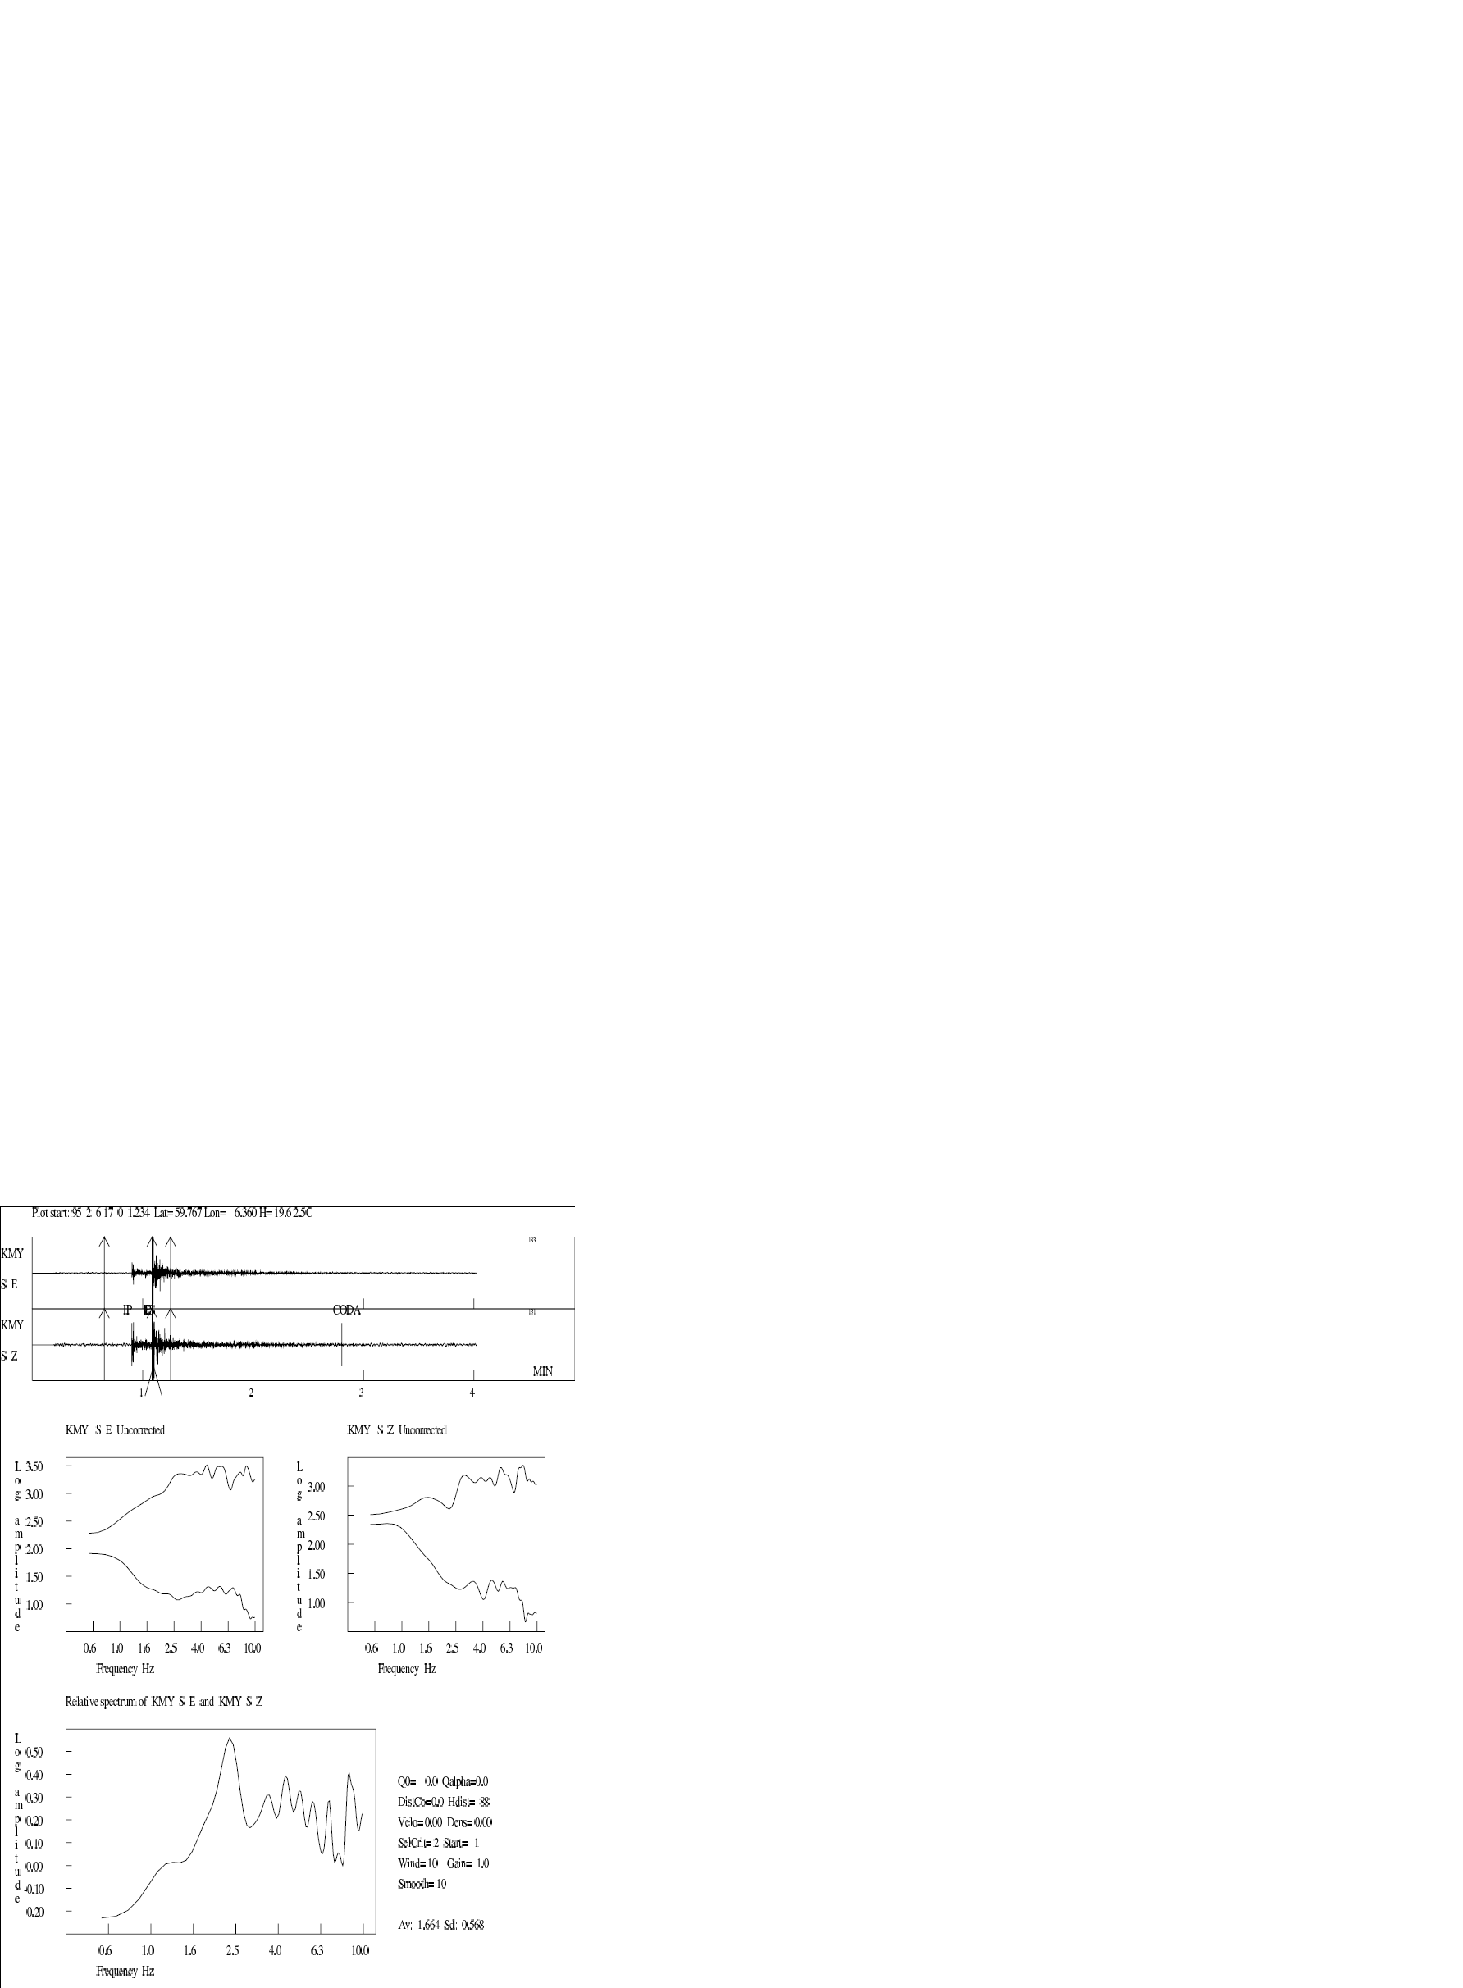
\includegraphics[width=0.9\linewidth]{fig/spec-example}}
\caption{
An example of using the SPEC program. On top the original traces are shown with windows chosen, in the middle the spectra of each channel and at the bottom, the relative spectrum. Lower right shows the input parameters used. In some cases (kappa and Q) the values calculated for this case are also shown.}
\label{fig:spec-example}
\end{figure}


\begin{figure}
\htmlimage{scale=2.0}
\centerline{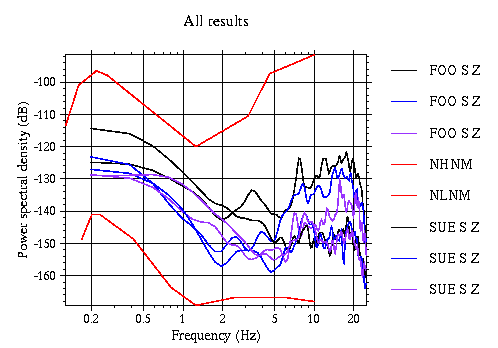
\includegraphics[width=0.9\linewidth]{fig/fig43}}
\caption{An example of a GMT plot. The figure shows an 
example of making noise spectra of several traces.}
%\label{fig:}
\end{figure}



\section{Seismic risk related programs} 
\label{sect:risk-prog}
\index{Seismic risk related programs} 

This section is written by \textbf{K. Atakan}. Extensive testing of the programs 
was done over the years by many users. \textbf{A.Ojeda}, performed testing 
and prepared input files for the CRISIS99 and CRIATT programs. 

\textbf{Introduction}

Currently, the SEISAN package includes a series of stand-alone programs that can be used in a number of tasks that are needed to perform seismic hazard analysis. The basic requirements for performing a \index{Probabilistic seismic hazard analysis}probabilistic seismic hazard analysis may be summarized as follows: 

Homogenize the earthquake catalogue and assess the completeness \newline
Define the \index{Seismic source zones}seismic source zones. \newline
Prepare input parameters from the \index{Earthquake catalogue}earthquake catalogue for each source zone. \newline
Prepare \index{Attenuation relations}attenuation relations for the region. \newline
Compute hazard in terms of peak ground acceleration (PGA). \newline
Assess \index{Site effects}site effects.\newline
Prepare \index{Seismic design spectra}response spectra. 

Following is a list of programs that constitutes the part of the SEISAN analysis package, which deals with seismic hazard and related problems. Most of these programs are described in more detail in different sections of the SEISAN manual. 

\textbf{SELECT}: Select a subset of earthquake data according to given criteria. \newline
\textbf{STATIS}: Statistical information about the database is computed and can be used in the analysis. \newline
\textbf{CATSTAT}: Program to compute and plot the yearly, monthly and daily number of events from a given catalogue. 
\newline
\textbf{CAT\_AGA}: Program to reorder the hypocenter lines in a CAT-file according to hypocenter agency in order to put the prime estimate in the beginning. \newline
\textbf{CLUSTER}: Program that searches for the dependant events in time and distance in a given earthquake catalogue. \newline
\textbf{EXFILTER}: Identifies the probable explosions, based on the 
user-defined parameters involving time-of-day distribution and the 
mining locations. It can be used for catalogue clean up and discrimination 
between the earthquakes and man-made explosions. \newline
\textbf{MAG}: Magnitude regression and conversion program. Prepares also a plot showing the scatter data and the best-fitted line. Magnitude conversions are then performed after a user defined priority list. \newline
\textbf{EPIMAP}: Plots coastlines, national boundaries and earthquake epicenters. It can also contour the produced output map file from hazard programs such as EQRISK, and overlay on the epicenter map. It is also possible to select a subset of earthquakes from a chosen polygon on the epicenter map. \newline
\textbf{BVALUE}: Prepares magnitude-frequency of occurrence diagrams and computes a- and b-values with maximum likelihood and least square approximation. In addition, the threshold magnitude and the maximum observed magnitude can be obtained. \newline
\textbf{CODAQ}: Computes the Q value from a given set of seismograms. This can be used later in the CRIATT program to create the attenuation table. \newline
\textbf{CRIATT}: Computes attenuation tables for a given set of parameters using the random vibration theory.\newline
\textbf{CRISIS99}:
\index{CRISIS99}
Computes seismic hazard in terms of the probability of exceedance vs earthquake intensity measures such as \index{Peak ground acceleration}peak ground acceleration (\index{PGA}PGA) or \index{Peak ground velocity}any other spectral ordinate. It can also compute hazard for a given grid of map co-ordinates corresponding to user-defined different return periods. (\textbf{SUN and PC}). The Windows program must be installed separately, look for ZIP file in SUP. \index{EQRISK}\newline
\textbf{EQRISK}: Program to compute seismic hazard in terms of probabilities of exceedances vs earthquake intensity measures such as peak ground acceleration (PGA), for a given site or a grid of sites for up to eight different return periods. Currently 1975 version is used. \newline
\textbf{EQRSEI}: 
\index{EQRSEI}
Converts the output file from the EQRISK program "eqrisk.out", to individual contour files corresponding to each return period specified. These files can later be used directly as an input to EPIMAP to plot the PGA contour maps. \newline
\textbf{SPEC}: Computes amplitude spectra for a given set of earthquake records and plots spectral ratios. It can be used to assess local site effects. 

Probabilistic earthquake hazard computations can be done, using the 
two alternative programs CRISIS99 or EQRISK. In addition, the programs 
listed above and a number of other programs that manipulates earthquake 
data within the SEISAN package, are useful tools to assess the parameters 
that are needed to perform a seismic hazard analysis for an area of 
interest. The two main programs, CRIATT for computing the attenuation 
tables and CRISIS99 (modified version 1999) to compute seismic hazard 
are explained in more detail in the following. Both programs are written 
by \textbf{Mario Ordaz} of the Institute of Engineering, UNAM \citep{ordaz1991,ordaz1999}. 
The well-known hazard program EQRISK, on the other hand, is written by 
\textbf{Robin K. McGuire} and the original manual is distributed through United States Department of the Interior, Geological Survey \citep{mcguire1976}.  

The two alternative hazard programs CRISIS99 and EQRISK have a number of features that are present in both. However, there are some advantages and disadvantages with both programs. In terms of the computing time and parameter input both programs require the same time. In the case of EQRISK, earthquake source zones are defined as arbitrary polygons (quadrilaterals). CRISIS99, on the other hand, operate with completely arbitrary polygons for the definition of the source zones and dipping planes may also be defined. In the MS-Windows 95 version, the source zones and the input parameters can be checked interactively through a user-friendly interface. In terms of the attenuation relations, CRISIS99 uses a table created by a separate program (CRIATT) and is therefore flexible (it also allows different attenuation relations for different source zones), whereas the attenuation relation, in the case of EQRISK, is given through a pre-determined mathematical formulation. Finally, CRISIS99 is superior to EQRISK, as it takes into account the uncertainties through the standard deviations introduced on several input parameters. 

\textbf{Step by step procedure for seismic hazard analysis}
\index{Seismic hazard analysis}

Following is a summary of the steps that have to be completed in order to produce a seismic hazard map. 

\begin{enumerate}
\item
 Compile a catalogue for the area of interest from local, regional and global sources. 
\item
 Evaluate the preliminary catalogue completeness by plotting histograms showing the distribution of events in time for different magnitude intervals. It may be necessary to divide your catalogue into two; 
(i) pre-instrumental and (ii) instrumental. Programs SELECT and CATSTAT can be used for this purpose. 
\item
 Convert magnitudes into one uniform magnitude, preferably to moment magnitude MW. To do this, regression curves must be prepared for different magnitude scales. Program MAG can be used for this purpose. 
\item
 Clean up the catalogue for dependant events (i.e. induced seismicity, non-earthquakes, foreshocks, aftershocks, earthquake swarms). Here a search has to be made for clusters of events both in time and space. Plots of histograms for specific sequences of time and space will reveal this. Program CLUSTER can be used for this purpose. The probable explosions may be removed by using the program EXFILTER. 
\item
 The evaluation of the catalogue completeness is dependent upon the clean-up process and the magnitude unification. It is therefore necessary that steps 2-4 be repeated until a reliable catalogue is prepared. 
\item
 Select the set of earthquakes from your catalogue from the part, which is complete for the chosen threshold magnitude and uniform in magnitude scale. Program SELECT can be used with different criteria for this purpose. Note the catalogue time span. 
\item
 Prepare a seismicity map for the area of interest with the selected data, using EPIMAP. Delineate the earthquake source zones. Here, zooming and the area selection procedures of EPIMAP may be used. 
\item
 Use additional information from geology, geophysics, seismotectonics, paleoseismology etc. to improve the source zonation. 
\item
 For each earthquake source zone select the subset of events that fall in the chosen area. This can be done by using the EPIMAP program, which enables to draw polygons interactively on the screen and put the subset of events within this polygon into a file. Alternatively SELECT program can be used to extract the subsets of data corresponding to the defined source zones.  
\item
 If the hazard is to be computed using CRISIS99 or by EQRISK, note the x, y (longitude, latitude), co-ordinates for each corner of the polygon. 
\item
 The seismicity within each source zone is assumed to be uniform following a Poissonian occurrence. In order to define this, a set of critical parameters has to be assessed for each source. These are: Number of earthquakes above a threshold magnitude: This is the \index{A-value}a-value for the lower bound magnitude. Catalogue time span: This is the time span of your catalogue where it is complete.  Beta (bvalue * ln (10)) and its standard deviation: The \index{B-value}b-value is the slope of the best-fitted line to the cumulative curve for the magnitude frequency of occurrence distribution (Gutenberg-Richter relation). \index{Maximum expected magnitude}Maximum expected magnitude with its standard deviation: This is usually inferred through other available information, such as geology, palaeoseismicity, or subjective judgement of the scientist. It is usually set to half a magnitude higher than the maximum observed when no information is available. \index{Maximum observed magnitude}Maximum observed magnitude: This is the largest magnitude observed within the catalogue time span. \index{Threshold magnitude}Threshold magnitude: The so-called \index{Lower bound magnitude}lower bound magnitude, which is chosen, based on the engineering considerations. Usually magnitudes less than 4.0 are not considered engineering significant. In order to obtain each of the above critical parameters, a thorough evaluation of the earthquake catalogue is needed. BVALUE program can\index{Catalog work} be used to obtain some of these parameters. However, while running the program, choosing the magnitude interval and the magnitude increment has to be done critically, taking into account the catalogue completeness and the detection threshold. These parameters will later be used in the input for the seismic hazard analysis program CRISIS99. Alternatively, the same input parameters are also needed for the EQRISK program. For each source zone, plot the magnitude- frequency of occurrence curves. 
\item
 Try to assess whether there are characteristic earthquakes in your 
region. This can be done with a careful examination of your catalogue 
and the active faults in the area. Studying the magnitude-frequency 
of occurrence through the BVALUE program will help assessing this. 
\item
 Try to establish an acceptable attenuation relation for your area. This can be done through empirical estimations or theoretically based on the random vibration theory (RVT). CRIATT program can be used to create the attenuation table. Alternatively, if you have an already established attenuation relation, this can be directly used in the EQRISK program. In this case, you can skip the steps 13-16, and continue from step 17 and onwards. 
\item
Establish a reliable Q factor by using the CODAQ program. This will be used in the attenuation program CRIATT to create the attenuation tables necessary for the hazard analysis. 
\item
 Create the necessary input file for the CRIATT by modifying the sample-input file `criatt.inp'. or use program CRIPAR.\index{CRIPAR} 
\item
 Run CRIATT to create the attenuation table necessary for the CRISIS99. 
\item
 Create the input file for the CRISIS99 program by modifying the example-input file `crisis99.inp'. Make sure that the critical parameters are reliable and the geometry of the source zones are correct (see the program description). 
\item
Run the CRISIS99 program with the input file you have created and the output attenuation table from CRIATT. The program will generate the output files with the probability of exceedance rate vs earthquake intensity (e.g. PGA), for the required return periods. Alternatively, if you have prepared the input for the EQRISK program, hazard can be computed by running the EQRISK program, for a given set of return periods (up to eight), for selected sites or for a grid of sites. 
\item
 Repeat stages 6 to 17 to refine your model and the corresponding results. 
\item
Convert the output hazard "map" file from CRISIS99 for the computed return periods to individual contour files. Alternatively, if you have used EQRISK to compute hazard, the output file "eqrisk.out" can be converted using EQRSEI program, into individual contour files for previously defined return periods. 
\item
Plot the hazard maps for the desired return periods. Contouring option from EPIMAP can be used for this purpose (only for the EQRISK). Plot also the graphs for probability of exceedance rates vs PGA for selected critical sites. 
\item
Try to assess the local site effects for the critical sites. SPEC program can be used to obtain the amplification factors due to unconsolidated sediments. These factors can be used later to adjust the response spectra. 
\end{enumerate}

Many of the programs mentioned above are described individually throughout this manual at different sections. In the following the programs that are directly relevant to hazard computations and not described in other sections of the manual are explained in detail. 

\textbf{CRISIS99}:
\index{CRISIS99}

CRISIS99 is a computer program to compute seismic hazard in extended 
regions. It was developed at the Institute of Engineering, UNAM, Mexico, 
by \textbf{Mario Ordaz} (mors@pumas.iingen.unam.mx), \textbf{Armando Aguilar} and \textbf{Jorge Arboleda}. 

Basic input data are: geometry of the sources, seismicity of the sources, and attenuation relations. Source geometry can be modeled as: 1) area sources, using a polygon with at least three vertex; longitude, latitude and depth must be given for each vertex, so this type of source can be used to model, for instance, dipping plates or vertical strike-slip faults; 2) fault sources, using polylines; and 3) point sources, included essentially for academic purposes. 

Seismicity of the sources can be modeled either as Poisson or characteristic earthquake process. In the first, magnitude frequency relations are smoothly truncated Gutenberg-Richter curves, whereas for the second, the program assumes a Gaussian distribution of the magnitudes. Hazard computations can be performed simultaneously for several intensity measures, for instance, PGA, PGV, and several spectral ordinates. Required attenuation laws are given in the form of tables containing the median values of the intensity measures as a function of magnitude (the rows of the table) and focal distance (the columns of the table). Several attenuation models can be used in the same run, assigning an attenuation pattern to each source. Using a recursive triangularization algorithm, spatial integrations are performed optimizing the number of calculations, so CRISIS99 will integrate with more points for the nearest sources and less (or none) for distant sources. 

CRISIS99 considers two different kinds of earthquake occurrence processes: Poisson process and characteristic earthquake process. CRISIS99 is oriented to computing hazard in extended regions. Hazard estimations are made for points in a grid that is not necessarily rectangular. The program can run under SunSOLARIS, SunOS and on PC (Windows95 or higher). Sun versions are to be used as a stand-alone program. The Windows version, on the other hand, also contains a windows interface for visual inspection of the input data as well as the results. Data validation options are available (only for the Windows version) and parameters can be given in a user-friendly graphic environment. CRISIS99 contains also a post-processing module that can be used to visualize the results, given in terms of maps of intensity measures for an arbitrary return period or exceedance rate curves for a selected site, not necessarily a point in the original grid of sites. Also, if several intensity measures are included in the computations, uniform-hazard spectra can be produced. The main results of a run are also written to ASCII files, so the user can use his/her own post-processing techniques/software. 

For the Windows version, a separate compressed file `crisis99.zip' is included with sample-input data in SUP. Instructions on how to install the Windows version are included in the file `crisis99.txt' in the INF directory. The Sun UNIX versions, are part of the standard SEISAN distribution and need not be installed specifically. 

Detailed description of the input and output files is given in the pages below. 

\textbf{Input files for the CRISIS99}
\index{Input files for the CRISIS99}

There are basically two input files that are required. First is an attenuation table (or several tables), and second is the major input parameter file where the file name for the attenuation table is also given. The input file can be prepared based on the format descriptions given below or modifying the example input file. An example-input file is included in the DAT directory with the file name "crisis99.inp". 

There are some limitations in the input parameters. Following is a summary of the maximum values set in the program: 

\begin{verbatim}
          Attenuation Models :                       5 
          Intensity levels*:                         20 
          Structural periods:                        15 
          Number of regions:                         200 
          Magnitudes in attenuation model:           10 
          Distances in attenuation model:            21 
          Number of sub-sources per region:          4000 
\end{verbatim}

(* the term 'intensity' here should not be mixed with macroseismic intensity. In this context 'intensity' is meant as any chosen ground motion measure, such as PGA, PGV or any other spectral ordinate). 

In the following the input file is described in more detail (by \textbf{Mario Ordaz}). 

I. GENERAL DATA FILE 

Format is free unless indicated otherwise. 

\begin{enumerate}
\item
General title of the run. 1 line \newline
TITGEN (A80) 
\item
Global parameters of the run. 1 line. \newline
NREG, NMOD, NT, NA \newline
NREG: Total number of regions (sources) in which the seismogenic area is divided. \newline
NMOD: Number of different attenuation models. \newline
NT: Number of spectral ordinates (or, in general, measures of intensity) 
for which seismic hazard is to be computed. \newline
NA: Number of levels of intensity for which seismic hazard will be computed. 
\item
Parameters for each spectral ordinate. NT lines. Free format \newline
T(I), AO(I), AU(I) \newline
T(I): Structural period of i-th spectral ordinate. It is used only 
for identification purposes, so in the cases in which structural 
period has no meaning, it can be just a sequential number. \newline
AO(I): Lower limit of intensity level for i-th spectral ordinate. \newline
AU(I): Upper limit of intensity level for i-th spectral ordinate. 
Exceedance rates for the i-th intensity will be computed at NA values, logarithmically spaced 
between AO(I) and AU(I) 
\item
More Global parameters \newline
RMAX, TR1, TR2, TR3, TR4, TR5 \newline
RMAX: Parameter 
controlling the spatial integration process. Sources at distances 
greater than RMAX kilometers from a site will be ignored. \newline
TR1,...,TR5: CRISIS-99 will generate a file containing intensity levels 
for fixed return periods TR1,...,TR5. See below for the description of this 
output file. Five values must be always given. 
\item
Parameters defining the basic grid of points in which hazard is to be computed. 1 line \newline
LOI, LAI, DLO, DLA, NLO, NLA LOI, \newline
LAI: Longitude and latitude, respectively, of the origin of the grid. \newline
DLO, DLA: Longitude and latitude increments \newline
NLO, NLA: Number of lines of the grid in the longitude and latitude directions, respectively. 

Results will be given for points (LO(I ),LA(I)), where 

LO(I) = LOI + (J-I)*DLO , J=1, NLO \newline
LA(I) = LAI + (I-1)*DLA, I=1, NLA 
\item
Number of polygons to be used to reduce the initial rectangular grid. 1 line. \newline
NPOLGRID 

Introducing one or more boundary polygons can reduce the initial rectangular grid of points. If  polygons are given (NPOLGRID>0) the computation of hazard will be performed only for those  points of the grid, which are inside one of the polygons. If NPOLGRID=0 computations will be  made for all points in the rectangular grid. NPOLGRID<=10. If NPOLGRID>0 then the following lines must be given for each polygon: 
\item
Definition of the k-th boundary polygon. \newline
NVERGRID (K) \newline
\parbox{.33\linewidth}{LONG (K, 1), LAT (K, 1) \\
\\
LONG (K, 1), LAT (K, 1)}
$\Bigg\}$ NVERGRID(K) lines 
%\hfill $\Bigg\}$ \hfill NVERGRID(K) lines \hfill
%\parbox{.3\linewidth}{}
%\parbox{.3\linewidth}{\verb|                 |}
%\parbox{.3\linewidth}{LONG (K, 1), LAT (K, 1)  LONG (K, 1), LAT (K, 1)}

NVERGIRD(K): Number of vertex of polygon k. NVERGRID(K)$<=3$0.\newline
LONG (K, I), LAT (K,I), I=1,...,NVERGRID(K): Co-ordinates of the polygon's vertex. 
The polygon must be described counter clockwise. 

\item
Files of attenuation tables. NMOD lines MODELO (I) (A20) 

MODELO (I): Name of the file containing the i-th attenuation table (including path). The  format of attenuation tables is explained below. 
\item
Data defining seismicity in each region. NREG blocks. \newline
TITULO (N) (A80) \newline
IC(N), IE(N), IMO(N) \newline
NV(N) \newline
%$\frac{LONG(1),LAT(1),PROF(I)}{\ldots} \bigg\}$ NV lines\newline
\parbox{.33\linewidth}{LONG(1),LAT(1),PROF(I) \\
\ldots}
$\bigg\}$ NV lines\newline
LONG(NV), LAT(NV), PROF(NV)\newline
Poisson model: (IC(N)=1)\newline
LAMBDA0(N), EB(N), CB(N), EMU(N), SMU(N), MMAX(N),M0(N)\newline
Characteristic model: (IC(N)=2) \newline
EMT(N), T00(N), D(N), F(N), SMT(N), M0(N), MU(N) 

TITULO(N): Identification name for source N \newline
IC(N): Flag defining the type of occurrence model assumed for N-th source. IC(N)=1 for Poisson model, IC(N)=2 for characteristic-earthquake model. \newline
IE(N): Defines type of source. IE(N)=0 for area source, IE(N)=1 for line source and IE(N)=2 for point source. \newline
IMO(N): Number of the attenuation model that will be used with this source. Must be between 1 and NMOD. \newline
NV(N): Number of vertex defining source N.

LONG(I), LAT(I), PROF(I), I=1,...,NV(N): Co-ordinates of vertex I of source N. LONG(I)  and LAT(I) are geographical coordinates of point i, whereas PROF(I) is the depth of the point,  in km, which must be positive.Sources can be of three types: areas (polygons), polylines or points. Polylines and points can be given in any order. In general, in the case of an area source, CRISIS99 will divide the polygon into triangles. It first checks if triangulation can be made in the XY plane. Numbering of the vertex of the polygon must be done counter-clockwise in this plane when looked from above the surface of the Earth. If there are vertical planes, CRISIS99 will try to triangulate the area in  the XZ plane, so numbering of vertex must be done counter-clockwise in this plane. Finally,  CRISIS99 will try to triangulate in the YZ plane. There are some bizarre source geometries  that cannot be well resolved by CRISIS-99, for instance, an L-shaped vertical plane. In these  cases, an error will be reported. 

Poisson model: \newline
LAMBDA0(N): Exceedance rate of magnitude M0(N). The units are earthquakes/year. \newline
EB(N), CB(N): Expectation and coefficient of variation, respectively, of the "b-value" for the source, given in terms of the natural logarithm. \newline
EMU(N), SMU(N): Expected value and standard deviation, respectively, of the maximum magnitude for the source. \newline
MMAX(N): Maximum observed magnitude in this source. \newline
M0(N): Threshold magnitude for source N. The catalogue of earthquakes is assumed to be  complete for M$>$M0. Earthquakes with M$<$M0 are absolutely ignored. 

Characteristic model: \newline
EMT(N): Median value of the times between characteristic earthquakes with M$>$M0. This is the inverse of the exceedance rate for M$>$M0. \newline
T00(N): Time elapsed since the last occurrence of a characteristic earthquake. \newline
D(N), F(N): Parameters defining the expected magnitude as a function of time, as in the slip�predictable model. It is assumed that 

E(M$|$t)=max(M0(N),D(N)+F(N)*LN(t)) 

Of course, if F(N) is set to zero, then D(N) becomes the expected time-independent magnitude of 
the characteristic earthquake. \newline
SMT(N): Standard deviation of the magnitude of the characteristic earthquake. It is assumed independent of time. \newline
M0(N): Minimum possible magnitude of a characteristic earthquake. Earthquakes with M<M0 are absolutely ignored \newline
MU(N): Maximum magnitude of the characteristic earthquake to be used in the integration process. 
\item
Name of the map file. 1 line \newline
File name (including path) containing the base map to be used in post-processing with CRISIS99 for windows. This name does not have any influence in the hazard computations. However, CRISIS99 expects a line here. 
\item
Name of the file of cities. 1 line \newline
File name (including path) containing the co-ordinates of cities, to be used in post-processing with 
CRISIS99 for windows. This name does not have any influence in the hazard computations. However, CRISIS99 expects a line here. 
\item
 ATTENUATION TABLES \newline
NMOD attenuation tables must be given each one in a different file. 
\end{enumerate}


The tables give to CRISIS99 the relations between magnitude, focal 
distance and median  intensities. CRISIS99 expects the following 
parameters in the i-th attenuation file, I=1,...,NMOD: 


\begin{enumerate}
\item
Parameters defining the magnitude limits. 1 line \newline
MINF(I), MSUP(I), NMAG(I) \newline
MINF(I): Lower limit of magnitude given in the table. \newline
MINF(I): Upper limit of magnitude given in the table. \newline
NMAG(I): Number of magnitudes for which intensity is given. 

CRISIS99 assumes than intensities are given for magnitudes M(K),  where M(K)=MINF(I)+(K-1)*DMAG, where DMAG=(MSUP(I)-MINF(I))/(NMAG(I)-1). 

\item
Parameters defining the distance limits. 1 line \newline
RINF(I): Lower limit of distance given in the table. \newline
RINF(I): Upper limit of distance given in the table. \newline
NRAD(I): Number of distances for which intensity is given. 

CRISIS-99 assumes than intensities are given for distances R(K),  where log(R(K))=log(RINF(I))+(K-1)*DLRAD, where DLRAD=(log(RSUP(I))-log(RINF(I)))/(NRAD(I)-1).  That is, distances are supposed to be logarithmically spaced. 

\item
For each of the NT different intensity measures, the following block 
of lines: \newline
T(I,J), SLA(I,J), AMAX(I,J) \newline
SA(I,1,1,1), SA(I,1,1,2),...,
SA(I,J,K,L),....,SA(I,NT,NMAG(I),NRAD(I) \newline
T(I,J): Structural period 
of j-th spectral ordinate. It is used only for identification purposes, so in the cases in which structural period has no meaning, it can be just a sequential number. SLA(I,J): Standard deviation of the natural logarithm of the j-th measure of intensity in the i-th model. \newline
AMAX(I,J): Maximum possible value of the j-th intensity in model I. The integration process will be truncated, regarding as impossible (zero probability) values larger than AMAX(I,J). If AMAX(I,J) is set to zero, then integration with respect to possible values of intensity will be performed from 0 to $\infty$. \newline
SA(I,J,K,M): Median value of the intensity in model I, for the J-th spectral ordinate, the K-th magnitude and the L-th distance. 


For each attenuation model, given in a separate file, CRISIS99 reads the above mentioned parameters in the following form: 

\begin{verbatim}
D0 J=1,NT
  READ(8,*) T(I,J),SLA(I,J),AMAX(I,J)
  DO K=1,NMAG(I)
    READ(8,*) (SA(I,J,K,L),L=1,NRAD(I))
  ENDDO
ENDDO 
\end{verbatim}

\end{enumerate}

Output files from CRISIS99 
\index{Output files from CRISIS99}

CRISIS99 generates several output files, whose names begin with the base name requested at the beginning of the run. The output files are: 

\begin{enumerate}
\item
Main results file. This file with - .res -extension contains a printout of the name of the run, the values assigned to the variables, characteristics of the attenuation models, geometrical and seismicity description of the sources, the data defining the computation grid, etc. It also gives the final results, that is, exceedance rates for each site and type of intensity. It also gives a brief 

summary of the computations for each site, indicating which sources are of interest to the site and which sources were skipped. 

\item
Graphics file. The principal graphics file with - .gra - extension 
contains a brief identification header, and the exceedance rates for 
the type and levels of intensity requested. This file can be used 
as input file to plot intensity versus exceedance rate curves. CRISIS99 
generates also a binary file with the exceedance rates for each structural 
period, so CRISIS99 will generate NT binary files. These binary files 
will be used only in the Windows System version of CRISIS99 to make 
hazard maps. The names of these files are base\_name.b1, base\_name.b2,..., base\_name.bNT. 

\item
Map file. This file with - .map - extension contains intensity levels for fixed return periods (TR1,...,TR5) for each type of intensity and site. It also gives the co-ordinates of each site. This file can be used to generate contour or 3d maps of intensity levels associated to constant exceedance rates. 
\end{enumerate}

Example output files are included in the DAT directory (crisis99.res, crisis99.gra, crisis99.map). 

CRIATT: 
\index{CRIATT}

In this program, an earthquake source model and results from Random Vibration Theory (RVT) \citep[e.g.,][]{boore1983,boore1989}, are used to estimate attenuation of ground motion parameters as a function of moment magnitude, MW, and hypocentral distance, R. Ground motion is assumed to be band-limited, stationary and of finite duration. 

For estimating the \index{Fourier acceleration spectra}Fourier acceleration spectra, a(f), it is assumed an \index{Omega square}omega square constant \index{Stress drop}stress drop source model given by \citet{brune1970}. The expression for a(f) is: 

\begin{equation} \label{eq:fas}
a(f) = CG (R) S(f) D(f) 
\end{equation}

where 

\begin{equation}
C = (4 \pi2 R_{V \phi} FV) / (4 \pi \rho\beta^3) 
\end{equation}

\begin{equation}
S(f) = M_0 f^2 / (1+f^2/f_0^2) 
\end{equation}

and 

\begin{equation} \label{eq:diminution}
D(f) = P(f) e^{-\pi R f / \beta Q(f)} 
\end{equation}

Thus the spectrum a(f) is the multiplication of a constant C (independent of frequency), \index{Geometrical spreading}geometrical spreading term G(R), \index{Source function}source function S(f), and \index{Diminution function}diminution function D(f). In C, Rv� is equal to average \index{Radiation pattern}radiation pattern (0.55), F is \index{Free surface effect}free surface effect (2.0), V is partition of a vector into two horizontal components (0.707), . is density in gm/cm3, and � is shear wave velocity in km/sec.  

In S(f), M0 is the \index{Moment}seismic moment and f0 is the \index{Corner frequency}corner frequency, given by \citet{brune1970}

\begin{equation}
f_0 = 4.9 x 10^6 \beta (\Delta \sigma / M_0)^{1/3} 
\end{equation}

where $\beta$ is in km/sec, $\Delta \sigma$ is the stress drop in bars, 
and $M_0$ is in dyne-cm. The diminution factor $D(f)$, accounts for loss 
of energy due to internal friction and scattering. 

At distances less than a certain critical value of 
$R_c$, the strong motion records are dominated by S-waves. 
Thus for $R < R_c$, $G(R) = 1/R$ is the geometrical spreading. 
For $R > Rc$, $G(R) = 1/(R R_c)^{1/2}$. 

The diminution function $D(f)$ in equation \ref{eq:diminution} requires $Q(f)$ and $P(f)$, 
where the \index{Quality factor}quality factor defined by the 
\index{Regional attenuation}regional attenuation is expressed by 
$Q(f) = Q_0 f^{\epsilon} $ ($f$ is frequency and $\epsilon \leq 1.0$), and whereas 

\begin{displaymath}
P(f) = e^{-\pi \kappa f} 
\end{displaymath}
(23) 

$P(f)$ reconcile an additional attenuation term which may be related to near-surface 
loss of energy where $kappa$ is a \index{High frequency decay factor}high frequency 
decay factor \citep{singh1982}. 

\textbf{Input file for CRIATT}
\index{Input file for CRIATT}

The standard input file for the CRIATT program can be created by modifying the 
example input file. A total of 23 parameters provide the necessary 
input for calculating the attenuation tables, which is based on 
equation \ref{eq:fas}, described earlier. The user should define the magnitude and 
the distance limits. It is important to note here that some combinations 
of parameters may result in 0 values for large distances in the table, 
which creates problems for the CRISIS99 program. In order to avoid 
this, the distance ranges are set to $R_{min}<10 km$ (CRISIS99 requires 
one-digit only) and $R_{max} < 500 km$. Usually the regional attenuation 
term and the site factor are the most critical factors in the definition 
of a(f). The effect of the high-frequency decay factor can only be 
seen when the combination of the kappa parameters ($kappa0$ and $kappa1$) 
are chosen correctly (e.g. increasing kappa1 with $kappa0$ kept constant, 
would result in low ground motion values). An example input file is 
included in the DAT directory with the file name \texttt{criatt.inp}. 

\index{Output file from CRIATT}
\textbf{Output file from CRIATT}

The output of the CRIATT program is a file containing the attenuation 
tables for the selected spectral ordinates (i.e. as a default only 
PGA corresponding to a period of $0.005 sec$ is computed). For each 
spectral ordinate, the file will contain a set of values (e.g. PGA) 
for different distances. This file is then used as one of the inputs 
to the CRISIS99 program. The file name is user defined. An example 
output file is included in the DAT directory with the file name \texttt{criatt.tab}. 

\textbf{CRIPAR} \newline
The program was used earlier to generate input for both crisis and criatt but now it is only used with criatt due a format change for crisis99.\index{CRIPAR} 

\index{EQRISK}
\textbf{EQRISK:}

This popular program for computing seismic hazard is written by \citet{mcguire1976}, and the complete manual is published as an open file report. The following is a short summary of the program operation and a full description of the input parameters as well as format of the input file. These descriptions are as they are given in the original manual \citep{mcguire1976}. 
The program EQRISK evaluates risk (hazard) for each site-source combination and intensity level and calculates the total annual expected number of occurrences of intensity greater than those levels of interest at a site by summing the expected numbers from all sources. Seismic source areas are specified as a set of arbitrarily shaped quadrilaterals. For ease of use, gross sources may be divided into sub-sources, which are a string of quadrilaterals, each two adjacent subsources having two common corners. A Cartesian co-ordinate system is used and the location of the origin is arbitrary. 

\index{Input file for EQRISK}
\textbf{Input file for EQRISK}

The default input file is named "DATA" and is hardwired into the program 
(for the SUN version file name should be uppercase). An example input 
file is included in the DAT directory with the name "eqrisk.inp", which 
should be renamed to "DATA" before running. Following is the description 
of the individual parameters and their format as described in the 
original manual \citep{mcguire1976}. 

\begin{itemize}
\item[Card 1] (Format 20A4): Title. Any 80 characters can be used 
to describe the problem. 

\item[Card 2] (Format 3I10): NSTEP, JCALC, JPRINT. \newline
NSTEP is the number of integration steps used in integrating over 
distance for each site-source combination. \newline
JCALC is the flag indicating how integration on magnitude is to be 
performed (JCALC=0 is used for analytical integration, and the form 
of the attenuation function is described in the original manual. 
JCALC=1 is used for numerical integration on magnitude. The user 
must supply own attenuation function in subroutine RISK2.) \newline
JPRNT is the flag indicating the desired output (JPRNT=0 is used to print only total expected numbers and risks at a site which is normally used when a grid of sites being examined. JPRNT=1 is used to print expected numbers from each site-source combination, normally used when examining a single site). 

\item[Card 3] (Format I5, 12F5.3): NLEI, TI(1), TI(2), ..... TI(NLEI). \newline
NLEI is the number of intensities to be examined. TI(1), TI(2) and so on, are intensities for which expected numbers and risks are calculated  at each site. Note, that the values for TI(i) may be Modified Mercalli Intensity or the natural logarithm of ground acceleration, velocity, displacement or spectral velocity. In printing results, the program prints both TI(i) and its antilogarithm. Values for array TI must be specified in increasing order. 

\item[Card 4] (Format 8F10.2): RISKS(1), RISKS(2), ..... RISKS(8). \newline
RISKS(1), RISKS(2), and so on are risks (probabilities of exceedance) for which the corresponding intensities are desired. These intensities are calculated by interpolation on a logarithmic scale, between intensities (in the list of examined intensities, TI) having larger and smaller risks. Both the corresponding intensity and its antilogarithm are printed. Values for array RISKS must be specified in order of decreasing risk. If fewer than eight values are desired, leave succeeding spaces on the card blank. To avoid large errors and subsequent misinterpretation, the program will not extrapolate to calculate intensity values corresponding to risk levels specified; it is the user's obligation to choose values for array TI which will result in risks which bound those specified in array RISKS. This is of course, a matter of judgement and experience. The user must be cautioned that in a grid site system appropriate values for array TI may vary considerably for the different sites examined. The intensities interpolated for levels specified in RISKS will be most accurate for closely spaced values of TI. 

\item[Card 5] (Format 8F10.2): C1, C2, C3, SIG, RZERO, RONE, \newline
AAA, BBB. C1, C2, C3 and RZERO are parameters in the \index{Attenuation equation}attenuation equation for mean intensity discussed in the original manual \citep{mcguire1976}: 
\begin{displaymath}
m_I(S,R)=C1+C2*S+C3*ALOG(R+RZERO) 
\end{displaymath}
SIG is the standard deviation of residuals about the mean. If no dispersion of residuals are desired, insert a very small value for SIG (rather than exactly 0.0). RONE is the limiting radius inside of which no attenuation of motion is desired, for values of focal distance closer than RONE, the mean intensity is calculated using RONE in place of R in the attenuation equation above. If this feature is not desired, insert zero for RONE. AAA and BBB are parameters in the equation limiting the mean intensity: 
\begin{displaymath}
max \, m_I(s)=AAA+BBB*S 
\end{displaymath}
The value specified for BBB must be between zero and C2 for this limiting equation to make sense. If it is not, an error message will result and program operation will terminate. 

\item[Card 6] (Format I10, 6F10.2): NGS, NRS(1), NRS(2), .... NRS(NGS). \newline
NGS is the number of gross sources to be specified. \newline
NRS(1), NRS(2), and so on are the number of subsources in gross source 1,2, etc. See the original manual \citep{mcguire1976}, for a general description of the source specification. 

\item[Card (set) 7] (Format I10, 6F10.2): LORS(I), COEF(I), AM0(I), AM1(I), BETA(I),  
     RATE(I), FDEPTH(I). \newline
There must be NGS+1 of these cards, one for each gross source and one for background seismicity. \newline
LORS(I) is a flag indicating whether the source area has a loose or strict lower 
bound (LORS=0 implies a loose lower bound and LORS=1 implies a strict lower bound). \newline
COEF(I) is a coefficient modifying the expected number of exceedances from gross source I. Its most common value is +1.0. AM0(I) is the loose or strict bound lower magnitude or intensity for gross source I. 
\newline
AM1(I) is the \index{Upper bound magnitude}upper bound magnitude or intensity for gross source 
I. 
\newline
BETA(I) is the value of $\beta$ for gross source I. It is equal to the 
natural logarithm of 10, times the Richter \index{B-value}b-value for the source. \newline
RATE(I) is the rate of occurrence of events having magnitudes of intensities greater than AM0(I). If a discrete distribution on intensities has been used to calculate the rate, the user may wish to specify AM0(I) as one-half intensity unit lower than the lowest intensity used to establish the rate. Note that for gross sources RATE(I) is in units of number per year; for \index{Background seismicity}background seismicity it is in units of number per year per 10,000 km. \newline
FDEPTH(I) is the focal depth of events in gross source I, in km. If epicentral distances are required for all sources and for background seismicity for the attenuation function, insert zero for FDEPTH(I). \newline
If no background seismicity is desired, leave the last card in this set completely blank. 

\item[Card 8] (Format 4F10.2): X1, Y1, X2, Y2. \newline
There must be NRS(1)+NRS(2)+ .... +NRS(NGS)+NGS of these cards. The first NRS(1)+1 cards specify co-ordinates of subsources in gross source 1, the next NRS(2)+1 cards specify co�ordinates of subsources for gross source 2, and so on. Internally, the point X1, Y1 is connected to X2, Y2, as well as both to the previous and the subsequent points designated as X1, Y1, as long as these are both in the same gross source. Point X2, Y2 is connected similarly. An example is elucidating. The following points define two gross sources having two subsources. 
\begin{verbatim}
 0.0  0.0 10.0  0.0 
 0.0  5.0  8.0  8.0 
-5.0 10.0  6.0 15.0 
10.0 20.0 11.0 20.0 
15.0 15.0 16.0 15.0 
15.0  0.0 16.0  0.0 
\end{verbatim}

\item[Card 9] (Format 2I5, 4F10.2): NX, NY, XZERO, YZERO, XDELTA, YDELTA. \newline
There can be any number of these cards, one for each site or grid of sites to be examined. 
NX and NY are the number of grid points in the X (East-West) and Y (North-South) directions; 
that is, they are the number of columns and rows in a grid of sites to be examined. For 
specification of a single site, NX and NY must have values of unit. Zero or negative values for NX 
and NY are meaningless and will cause program to terminate. \newline
XZERO and YZERO are the co-ordinates of the site to be examined, or are the lower left corner 
of the grid if NX and/or NY are greater than one. \newline
XDELTA and YDELTA are the grid spacing in the X and Y directions. When the grid option is not 
used, these variables may be left blank or set equal to zero. 

\item[Final card:] Insert one blank card at the end of the input deck. 
\end{itemize}

\index{Output file from EQRISK}
\textbf{Output file from EQRISK}

There is only one standard output file generated by EQRISK which has a default file name of "eqrisk.out". This file contains the results of the hazard computations for each site for the specified exceedance probabilities. This output file can easily be converted to individual intensity (e.g. PGA) contour files (one for each level of exceedance probability), using the program EQRSEI. The resulting \index{Contour maps}contour maps from these output files may then be plotted by EPIMAP. 

The detailed format of this output file is described in the original manual \citep{mcguire1976}, and is not repeated here. A test set of input and output files are given in DAT.  

\index{EQRSEI}
\textbf{EQRSEI:}

The program EQRSEI converts the output file \texttt{eqrisk.out} from the EQRISK program into individual intensity contour files for the previously defined return periods. There may be up to eight such files (eqrsei1.out, eqrsei2.out ...., eqrsei8.out). These files can then be used as input to the EPIMAP program to plot the contours of PGA values on the epicenter maps. Each file contains also some header information, where the individual contours and the contour intervals are given. In addition, the color codes are also given. The individual contours and the contour intervals can be modified by editing the header lines of these files. 

\index{CLUSTER}
\textbf{CLUSTER:}

This is a program that searches for the dependant events in a given catalogue (compact file) with respect to time and distance. It is written by Juan Pablo Ligorr�ia and Conrad Lindholm. The input is a standard Nordic file with header lines only (compact file). The user has to give the number of days to be searched before and after the main event, and the distance limits in km. The magnitude of the main event over which the search will be performed is also user defined. The output is a repetition of the input catalogue with "?" placed at the end of each dependant event which falls within the limits defined in the interactive input in time and distance. The default file name is \texttt{cluster.out}. The user should then work systematically through these events and decide whether they should be cleaned or not. This process, we feel, should be done manually, because deleting events from the catalogue (especially the historical part), may have serious implications later in the hazard computations. Clusters of foreshocks, aftershocks or other dependant events such as earthquake swarms can be delineated by this program. 




\section{Magnitude relations, MAG} 

The MAG program\index{MAG} calculates simple \index{Magnitude relation}magnitude relations. The program has three functions: (1) Calculate parameters for a magnitude scale (\index{Ml}Ml or \index{Mc}Mc), (2) Calculate relation between two different magnitudes and/or spectral parameters and (3) Calculate a new magnitude as a function of an existing magnitude, a natural step following function (2). All three functions can be done at the same time. Function (3) can also be used for moving a particular magnitude type and/or agency to the first magnitude position in line 1 to be plotted with EPIMAP. \index{Magnitude} 

ALL HEADER LINES ARE SEARCHED FOR MAGNITUDE INFORMATION 

Input: The data input is a CAT-file like one made with SELECT or COLLECT or it can be a compact file if only magnitude comparison is made. Optionally there can be a parameter file, which MUST be, called mag.par and MUST reside in the working directory. An example of the parameter file is found in DAT and also shown below. The parameter file is not needed for all operations, see details below. 

1: Magnitude scales 

Coda magnitude Mc: The coda magnitude scale used is 

\begin{displaymath}
Mc = A * log(coda) + B * dist + C 
\end{displaymath}

where \index{Mc}Mc is the coda magnitude, coda is the \index{Coda length}coda length in secs, dist is the hypocentral distance in km (calculated from epicentral distance and depth in CAT file) and A, B and C are constants to be determined. This is done in two ways 

3d regression 

\begin{displaymath}
m = A * log (coda) + B * dist + C 
\end{displaymath}

2d regression 

\begin{displaymath}
m = A * (log (coda) + dist\_coff * dist) + C 
\end{displaymath}

with B = A * dist\_coff where dist\_coff is given in the parameter file and m is the reference magnitude. SO B AND dist\_coff ARE DIFFERENT. The CAT-file must contain coda readings, epicentral distances and a magnitude in the header line. A linear regression is then made between the known magnitude from a given agency and the observed coda lengths following the relations above. The user has the option to choose the type of magnitude to use in the regression. Usually Ml or Mb are used. All station-event combinations are used to determine simultaneously the 3 constants A, B and 
C. Since the data often is too bad to determine all 3 parameters at the same time, the program will also calculate just A and C using a fixed user supplied value for the distance correction to the coda. 
The constant dist\_coff is given in the mag.par file as the second parameter under MAG\_TYP\_COF (see below). IN ORDER FOR THE CODA SCALE OPTION TO WORK, THE DISTANCE COEFFICIENT MUST BE DIFFERENT FROM ZERO. 

Output: On the screen the constants will be printed out and a file mag\_coda.out will contain pairs of values m and (log(coda) + dist\_coff*dist), which can be used to plot the distance corrected coda relation. If results from the 3D is to be plotted, dist\_coff must be calculated as dist\_coff=B/A, put into mag.par and mag run again. On the other hand, if a best dist\_cof has been found, B is calculated as B=A*dist\_cod 

A typical coda magnitude relation is :

\begin{displaymath}
Mc = 2.0*log(coda) + 0.0035*dist - 0.87 
\end{displaymath}
\citep{lee1972} 

Local magnitude \index{Ml}Ml: \newline
The local magnitude scale is calculated by determining an amplitude attenuation scale using amplitudes and distances in CAT file. The parameters in the Ml magnitude scale are computed for every event individually, parameters are determined as averages of all events. 

For each event (only type L and R are used) a,b,c are calculated if at least 3 stations are available 
using least squares regression as follows: 

\begin{displaymath}
log(amp) = a * log(dist) + b * dist + c \index{Amplitude attenuation}\index{Quality factor} 
\end{displaymath}

The relation above can be derived from the standard geometrical spreading and attenuation relations: 

\begin{displaymath}
amp = (dist ** a) * exp(pi * f * dist/(v*q )) 
\end{displaymath}

where $f$ is the frequency, $v$ is the velocity and $q = q0*f**qalpha$. The relation can be rewritten 

\begin{displaymath}
log(amp) = a * log(dist) + (pi * f * dist) /(v * q0*f**qalpha * 2.3) 
\end{displaymath}

Since $qalpha$ often is close to $1.0$, the relation can be simplified to the frequency independent relation:

\begin{displaymath}
log(amp) = a * log(dist) + (pi * dist) /(v * q0 * 2.3) 
\end{displaymath}

If body wave spreading is assumed $(a=1)$, $q0=100$ and $v=3.5 km/sec$, the relation is 

\begin{displaymath}
log(amp) = 1.0 * log(dist) + 0.004 * dist 
\end{displaymath}

which is comparable to the relation shown below for California. 

Similarly to the coda relation, a 2D relation is also calculated 

\begin{displaymath}
log(amp) - b*dist = a * log(dist) 
\end{displaymath}

where $b=dist\_coff$ is fixed to the value given in the mag.par file (same parameter as used for coda). This gives a more stable solution, however b = dist\_coff must be determined by trial and error or fixed using known values from e.g. q-studies.\index{Geometrical spreading} 

The amplitudes are assumed to be ground displacements (in SEISAN they are \index{Ground displacement}ground displacements highpass filtered at 1.25 Hz to resemble \index{Wood Anderson}Wood Anderson seismograms, see MULPLT). The distance ratio between stations with the maximum distance and minimum distance must be more than 3 for the event to be selected for analysis. It is assumed that a and b will be the same for all events, while c is different (magnitude dependent). At the end, the average constants a and b are calculated of all values a and b which are not deviating too much (a must be in the range 0 to -5, hardwired). Distance attenuation coefficients a and b are supposed to be negative since amplitude decrease with distance. To get the \index{Local magnitude}local magnitude scale 

\begin{displaymath}
Ml = log(amp) - a * log(dist) - b * dist - C 
\end{displaymath}

the constant C must be determined by fixing the magnitude at some 
reference distance like the original Wood Anderson definition with 
$Ml = 3$ at $dist= 100 km$ and $amp=1/2200 mm = 454 nm$ (assuming gain of 
the Wood Anderson seismograph to be 2080, \citep{hutton1987}. 
The determination of a and b does not work well unless the observations 
are very good. The relation for California is \citep{hutton1987}

\begin{displaymath}
Ml = log(amp) + 1.1 *log(dist) + 0.00189 * dist - 2.09 
\end{displaymath}

Output: On the screen the constants will be printed out and a file mag\_amp.out will contain the values of a, b and c. 

2: Magnitude relations and/or spectral parameter relations 

Linear regression (maximum likelihood) can be made between any two magnitudes and/or spectral parameters on any of the header lines of an event in a CAT-file or a compact file. The user is interactively prompted for the magnitude type and/or spectral parameters and agencies to compare. If none is given, no magnitude comparison will be made. If several magnitudes/spectral parameters fit the requirement, the last one is used. If e.g. the first header line has a BER Ml and the last header line also has a BER Ml, the last one will be used.  Maximum likelihood linear fitting is used. It is assumed that both variables have normal and correlated errors. See subroutine maxlik.for in LIB for more info. 

The following parameter can be selected: 

Any magnitude and agency \newline
Seismic moment(log) \newline
Stress drop (log) \newline
Corner frequency (log) \newline
Source radius(log) \newline
Spectral decay \newline
Omega zero level (log) 

If any of the spectral parameters are selected, or  moment magnitude is without agency, there will be an additional question about which station and component. A blank return means the average will be used. With these parameter selections, it is possible to compare spectral parameters from any two channels, compare the average spectral parameter with the parameter from one channel etc. 

Output: A plot will be shown on the screen with the observations and the least squares fit and the values are also printed out on the screen. A file mag\_mag.out contains the pairs of magnitudes used. 

3: \index{Magnitude conversion}Magnitude conversions 

If a relation between two magnitude scales is known, e.g. by using option 2 above, an output file can be made with the \index{Converted magnitude}converted magnitudes. The relation to use is specified in the mag.par file. Several different input magnitude types and agencies can be used and the relation-agency used is given in a priority list in the mag.par file, see example below. It is here shown that if a BER Mc is available, this will be the first choice. If no BER Mc then BER Mb will be the next choice etc. The new magnitude will have type X and \index{Agency}agency NEW. Output: The output file is mag\_new.out and has the same format as the input file. On the header line, the old magnitudes are removed and in the first magnitude position will be the converted magnitude (NEW) while in the second magnitude position, the magnitude selected for \index{Mag\_amp.out}\index{Mag\_coda.out}\index{Mag\_mag.out}\index{Mag\_new.out}\index{Mag\_newa.out}\index{Mag\_spec.out}\index{Spectral parameters}conversion will be given. The third magnitude position is blanked out. The conversion option can also be used to move magnitudes around by using a 1 to 1 relation as shown in mag.par example. 

Summary of output files: 

\begin{tabular}{lp{10cm}}
\texttt{mag\_amp.out} : & Details each event for amplitude regression. \\
\texttt{mag\_coda.out} : & Magnitude vs coda, see text. \\
\texttt{mag\_mag.out} : & Pairs of magnitudes used for regression. \\
\texttt{mag\_new.out} : & Events with converted magnitudes only. \\
\texttt{mag\_newa.out} : & All events, both converted and non converted (due to no correct input     magnitude available). \\
\texttt{mag\_spec.out} : & Summary of normal header line, all associated magnitudes    and spectral parameters. \\
\texttt{mag\_ml\_inv.out} : & From Ml inversion \\
\end{tabular}

In DAT there is an example \texttt{mag.par} file. 

\begin{figure}
\htmlimage{scale=2.0}
\centerline{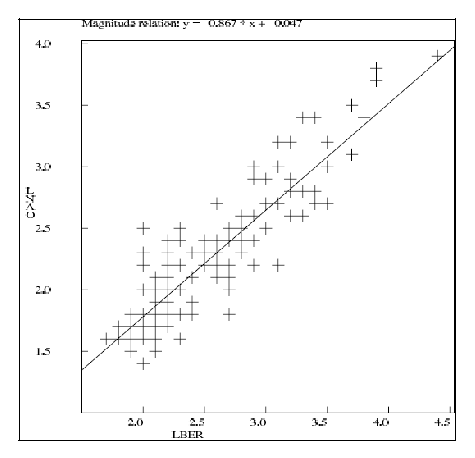
\includegraphics[width=0.9\linewidth]{fig/fig44}}
\caption{Example of using the MAG program. 
Relation between NORSAR and Bergen local magnitudes.}
%\label{fig:}
\end{figure}

An example of the \texttt{mag.par} parameter file: 

\verbatiminput{include/mag.par}


% nov 21 2012 jh: added a bit to the the Ml ref. distance
%
\section{ML inversion, MAG2}
\index{MAG2}
\label{MAG2}

MAG2 is a program to invert for the local magnitude scale ML. 
The difference to the inversion done in MAG is that MAG2 inverts 
amplitudes from all events simultaneously for the scale and 
station corrections. The program can invert for different scale 
parameters depending on selected distance ranges. The reason for 
this is that it is known that the geometrical spreading is not 
the same for example between Pg and Pn. Some authors have suggested 
distance dependent scales, but most commonly a single scale is used 
for all distances for simplicity.

The general ML scale is given by 

\begin{displaymath}
ML = log_{10} A + a log_{10}(R) + b R + S + c
\end{displaymath}

where we measure the displacement amplitude A in nm, R is the hypocentral 
distance in km, S is the station correction of the individual stations, 
and c is a constant added to make the scale comparable to other places at a 
reference distance. The station corrections add up to 0. The region 
dependant parameters in the scale are a, accounting for geometrical 
spreading, and b, accounting for attenuation. The part 
$(a log_{10}(R) + b R + c)$ is commonly written as $(-log_{10} A0)$. 

The program applies singular value decomposition using 
the Numerical Recipe \citep{press2003} routines to invert 
the observations for a, b and S. It then computes the parameter 
c based on the reference given through distance, amplitude and 
magnitude. This allows to calibrate scales between different 
regions so that they are the same at the reference distance. 
Commonly c is set such that 480 nm amplitude at 17 km gives ML=2 
(this is equivalent to 1 mm on a Wood-Anderson seismograph 
giving ML=2 at 17 km \citep{hutton1987}. The original definition was 480 nm at 100 km giving a ML=3 (equivalent to 1 mm on a Wood-Anderson seismograph at 100 km distance), however it is now considred that a shorter reference distance will give a more accurate scale. The inversion 
can be setup to invert for the geometrical spreading  term a 
in the scale for up to three distance ranges. However, a single 
attenuation term b is used.

As input the program requires a parameter file mag2.par in the 
working directory,and a standard station file e.g. STATION0.HYP. 
Then the user only has to enter the input file of events in Nordic 
format. An example file, mag2.par, and an input file, mag2nor.cat, 
with events from Norway are in given in DAT., 

The parameter file has the following settings given by keywords (any order):

INVERSION TYPE (f10.1) - 1. = singular value decomposition (no other choice yet)\newline
DISTANCES (2f10.1) - distance range in km for observations to use\newline
MINIMUM NUMBER OF OBS/EVEN (f10.1) - only events with more or equal number 
of observations are used\newline
MIN DISTANCERANGE RATIO (f10.1) - minimum range required computed as ratio 
of distances defined by DISTANCES\newline
ORIENTATION (f10.1) - use of components: 0. = horizontal and vertical, 
1. = horizontal only, 2. = vertical only\newline
SYNTHETIC (f10.1) - set to 1. for synthetic test, scale defined by FIX SCALE A and FIX SCALE B; 0. for inversion of data\newline
NOISE (f10.1) - ratio of amplitude to be added as noise to synthetic test\newline
FIX SCALE A (3f10.1) - set the fixed parameter a in scale, possible for the 
three distance ranges given by SCALE DISTANCE\newline
FIX SCALE B (3f10.1) - set the fixed b parameter in scale, possible for the 
three distance ranges given by SCALE DISTANCE\newline
FIX SITE (f10.1) - set to 1. to not invert for station corrections; 0. for 
default inversion for station corrections\newline
REFERENCE DISTANCE, REFERENCE AMPLITUDE, REFERENCE MAGNITUDE 
(all f10.1) - setup of the reference, used to calculate parameter c, 
give amplitude as Wood Anderson amplitude in mm\newline
SCALE DISTANCE (2f10.1) - give up to two distances which give the 
transition between the possibly three distance dependent scales; blank 
or numbers larger than maximum distance will give only one scale\newline
IGNORE COMP (a4)  - give component not to be used\newline
IGNORE STAT (a5) - give station not to be used\newline


The program produces a number of output files:

mag2\_amp\_dis.out - amplitude versus distance for each event\newline
mag2\_amp\_obs.out - list of observed amplitudes\newline
mag2\_events\_read.out - listing of events that were read in\newline
mag2\_events\_used.out - events used in Nordic format\newline
mag2\_evxy.out - coordinates of events used\newline
mag2.out - general output file, lists data used and computed scale\newline
mag2\_paths.out - event-station path coordinates\newline
mag2\_station\_hyp.out - hyp station file with scale and station corrections\newline
mag2\_stat\_list.out - simple output of stations used\newline
mag2\_statxy.out - coordinates of stations used\newline

The output file mag2.out will give some details on the input data, as number of 
stations, events and observations. It reports the reference used to fix the scale at 
the reference distance. Next it gives the scale, consisting of three parts if inversion 
is done for all possible segments. This will be given by a1, a2, a3, while b will be 
assumed to be the same. First the scale is presented to include the reference distance, 
second it is shown without the reference distance included with the scale. Then comes a 
section with the stations and the respective site terms, and finally the list of events 
with the source term inverted for.

The output file mag2.out for the example in the DAT directory should look like this:

\begin{verbatim}
ML inversion output

 SVD inversion

 Total number of events:           69
 Total number of stations:           23
 Total number of observations:          600

 Reference distance  =    100.0000    
 Reference amplitude =    1.000000    
 Reference magnitude =    3.000000    

 Ml = log A + a log(dist/refdist) + b (dist-refdist) + c + S 
     a1=  0.84717 +/-  0.39844
     a2=  0.00000 +/-  0.00100
     a3=  0.00000 +/-  0.00100
     b =  0.00061 +/-  0.00136
     c =  0.31807 +/-  0.00000

 Ml = log A + a log(dist) + b (dist) + c + S 
    a1 =  0.84717 +/-  0.39844
    a2 =  0.00000 +/-  0.00100
    a3 =  0.00000 +/-  0.00100                                                                    
     b =  0.00061 +/-  0.00136
    c1 = -1.43679
    c2 =  0.25756
    c3 =  0.25756

Station #    1 STAV  -0.120  +/- 0.2612   58.935    5.702
Station #    2 BLS5  -0.044  +/- 0.2204   59.423    6.456
Station #    3 ODD1  -0.085  +/- 0.2125   59.911    6.627
Station #    4 EGD    0.043  +/- 0.2221   60.270    5.223
...
Station #   21 MOR8  -0.018  +/- 1.3061   66.285   14.732
Station #   22 ESK    0.851  +/- 1.1257   55.317   -3.205
Station #   23 AKN    0.171  +/- 0.3797   62.178    6.997
 Average site term:   0.00
  Event #     1 2002051922484590  ML =  1.95 +/- 0.438
  Event #     2 2002052614481700  ML =  1.68 +/- 0.577
...
\end{verbatim}


\subsection{MAGSTAT}
\index{MAGSTAT}
\label{MAGSTAT}

The program MAGSTAT can be used with MAG2 to produce statistics that 
allow to evaluate the magnitude scale. 
As input it takes a STATION file, as produced by MAG2, and a Nordic 
input file. Here, one can use any data set, 
or the events that were used in the MAG2 inversion.

This program is still under construction. 






\section{Explosion filtering, EXFILTER} 
\label{sect:exfilter}

\index{Explosion filtering}\index{EXFILTER}\index{Catalog work} The program EXFILTER is used to identify probable explosions in a catalog of seismic events. Man-made seismic events like quarry blasts, mining explosions and other explosions show a certain distribution in time and space. Therefore the method of explosion identification here is based on normalizing the time of day distribution of seismic event occurrence as a function of area. The program works on the following principle: Areas where explosions occur are defined. If an event is located in one of these areas, with a magnitude below a given maximum magnitude, with a depth less than a given maximum depth, within a given time of day interval and within a given year interval, it is identified and marked as probable explosion. The areas are defined by \index{Polygon}polygons of any shape. For definition of the filter areas, a list of mine locations (with consideration of location accuracy), locations of explosions and locations of event clusters (they might be clearly related to mine locations, but others might indicate unknown explosion sites) can be used. The next step is to define the parameters for each area to get a normal time of day distribution. They can be determined following the steps: 

\begin{itemize}
\item[1)]
\begin{itemize}
\item[]
- get the time of day distribution of events (program CATSTAT) 
\item[]
- select a time window of probable explosions 
\item[]
- select events within time window of probable explosions 
\end{itemize}
\item[2)]
\begin{itemize}
\item[]
- get the distribution of magnitudes of events within time window of probable explosions (program BVALUE) 
\item[]
- select the maximum magnitude 
\end{itemize}
\item[3)]
\begin{itemize}
\item[]
- test parameters defined with program EXFILTER for the defined area and adjust the parameters if the time of day distribution is not normal. 
\end{itemize}
\end{itemize}

For more details, see \citet{ottemoller1995}.

The program uses a parameter file, \texttt{EXFILTER.PAR} which MUST be located in the DAT directory. 

An example of the parameter file \texttt{EXFILTER.PAR}

\verbatiminput{include/exfilter.par}

The EXFILTER program searches for probable explosions using a 
catalog-file as input and marks events that might be explosions with 
'P' as Event ID in the output file \texttt{exfilter.out}. 
Example of program run 

\begin{verbatim}
<exfilter> 

NUMBER OF AREAS: 55 

 FILENAME... ? 
june.cat
 ************************************
 Number of probable explosions found: 90
 Output written in file: exfilter.out
 ************************************ 
\end{verbatim}

\begin{figure}
\htmlimage{scale=2.0}
\centerline{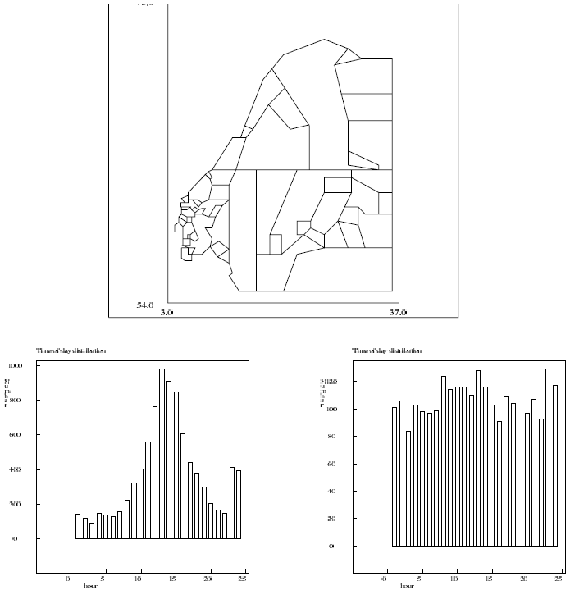
\includegraphics[width=0.9\linewidth]{fig/fig45}}
\caption{Figures that show how the exfilter works for events in Scandinavia:\newline
The top figure shows the filter areas used for Scandinavia. The bottom right figure shows the time of day distribution for a 10 year Scandinavian catalog before filtering (made with CATSTAT) and the figure bottom left shows the distribution after filtering.}
\label{fig:exfilter}
\end{figure}




\section{Inversion of travel time data and joint hypocenter determination} 


\subsection{VELEST} 

\textbf{Introduction}

The program \index{VELEST}VELEST is used to solve the coupled hypocenter velocity model problem for local earthquakes. It performs a simultaneous inv\index{Inversion}\index{Joint hypocenter determination}\index{JHD}ersion for hypocenters and velocity model. The inversion is limited to first arriving phases. A detailed program description is given in the `VELEST USER'S GUIDE' \citep{kissling1995}. A recipe for preparing data and use of the inversion routine is presented in `Initial reference models in local earthquake tomography' \citep{kissling1994}. The two documents are available in one Postscript file in the INF directory, the filename is `velest.ps'. The derived model can be used as an improved model for earthquake location or as a starting model for 3-D inversion. For a fixed velocity model and constant station corrections, VELEST in simultaneous mode performs the Joint-Hypocenter-Determination (JHD). 

%\textcolor{red}{lo-change:
Before you start please see the two articles Kissling-1988.pdf and Kisslig-1994.pdf in the INF directory.
%}

The original version of VELEST by Kissling is included in the Sun and Linux versions. A version modified to compile VELEST under Windows has been provided by Freddy Aldersons (e-mail: faldersons@earthlink.net). This Windows package is included in the file velest\_pc\_3.3.zip, which is located in the SUP directory. The files have to be extracted to the PRO directory.\index{Velest for Windows} 

The implementation of VELEST to SEISAN is given by the program VELMENU.  

\index{VELMENU}
VELMENU provides: 
\begin{itemize}
\item[-]
automatic format conversion to VELEST 
\item[-]
generation of parameter files using the SEISAN system 
\item[-]
execution of VELEST 
\item[-]
conversion back to SEISAN format 
\end{itemize}

After preparing a dataset of local earthquake data, VELMENU can be used to work with the VELEST inversion routine. The first time VELMENU is used, all input files for the inversion with default parameters can be generated. These parameter files then can be changed interactively and the inversion started with VELMENU. 

\textbf{Running VELMENU}

The program is started with `velmenu'. After entering the filename of the earthquake data the menu of VELMENU appears. 

Example of program run : 

\begin{verbatim}
velmenu 

File name of earthquake data in Nordic Format :
select.out 

VELEST MENU 
-----------

1. Create VELEST command file (vele\index{Velest.cmn}st.cmn)
2. Edit/change VELEST command file (velest.cmn)
3. Create station select file (selstat.lis)
4. Edit/change station select file (\index{Selstat.lis}selstat.lis)
5. Create model file 
6. Edit/change model file
A. RUN VELEST 
B. Edit inversion output file
C. Convert VELEST output to Nordic format and make diff-file 
Q. End 

Choice ? 
\end{verbatim}

The complete inversion-process of earthquake data in SEISAN format, including all conversions and preparation of parameter files, can be done with VELMENU. The steps are as follows:   

\begin{itemize}
\item[1:]
Create VELEST command file (\texttt{velest.cmn}) \newline
The user is asked for inversion or JHD and the appropriate parameters 
are set. The file \texttt{velest.cmn} is the central VELEST parameter 
file. To create it, the file of earthquake data is read to determine 
the parameters that depend on the data. These are the number of events 
and the center of Cartesian coordinate system, which is simply determined as the average of latitude and longitude of epicenter locations. The remaining parameters are set to default values. 
\item[3:]
Create station select file (\texttt{selstat.lis}) \newline
For the inversion, VELEST will use phases from stations with an 
epicentral distance below a maximum distance only. In addition in 
VELMENU a selection of stations has to be used, only phases from 
stations given in the file \texttt{selstat.lis} will be used for inversion. 
When generating the file, the maximum distance between station and 
hypocenter (parameter `dmax') is read from \texttt{velest.cmn} and 
the input data are scanned to get a list of stations, which are within the 
limit to any epicenter. Editing the file, stations can be added or removed. 
If all stations should be used for inversion, the parameter `dmax' in 
the file \texttt{velest.cmn} has to be increased. 

Example of \texttt{selstat.lis}:
\begin{verbatim}
#
# STATION SELECT FILE FOR PROGRAM VELEST 
#
# STATIONS WILL BE USED IN THE VELEST 
#      INVERSION PROGRAM 
# 
# COMMENT LINES START WITH 
# 
#
KONO
BER
NRA0
... 
\end{verbatim}
NOTE: The order of the stations is as given by the input data file. VELEST uses the last station as reference station, so you may want to change the order. 
\item[5:]
Create model file \newline
The input model file `model.inp' is created using the model as given in the `\texttt{STATION0.HYP}' file. The `\texttt{STATION0.HYP}' file, if available, will be read from the local directory, otherwise from the DAT directory. This might be a reasonable starting model, but of course the model file has to be changed. 
\end{itemize}

A. RUN VELEST 

Once the parameter files are created the inversion program can be started. The inversion study requires interactive changing of parameters, which is supported by VELMENU. All input parameter files can be changed from VELMENU. NOTE:, `... please accept the warning: To calculate a Minimum 1-D model a single or even a few VELEST runs are useless, as they normally do not provide any information on the model space!' \citep{kissling1995}. The conversions and the inversion programs are started as one process. 

Before the inversion routine is started the station locations will be converted from the \texttt{STATION0.HYP} file and the earthquake data in Nordic format will be converted to CNV (hypocenters and travel times) format. NOTE: VELEST does not support 5 character station codes, therefore in the conversion to VELEST, only the first 4 characters are used if the station code has 5 characters. In the conversion of the earthquake data only phase readings from stations included in the station selection file will be used. Arrivals with a time residual, given in the Nordic input file, above five seconds are omitted. Only the first arriving phase of P and S respectively are used. The hypocenter location given by the inversion will be determined by first arrivals only. The original data might include more phases like Pg, Sg or Lg. Therefore, to get a comparison of hypocenter locations between the HYP location program and VELEST, a Nordic file including the same data as the CNV file is created and the HYP program run on this file before VELEST is started. The HYP program can be skipped by pressing `CTRL+C', while it is running. 

The results of the inversion will be given in a text file that can be 
viewed within VELMENU. VELMENU provides an option to convert the VELEST 
output file with final hypocenter locations in CNV format back to 
Nordic format and to write a file that shows differences 
(\index{Velout.dif}\texttt{velout.dif}) in location and time between 
the two location routines, HYP and VELEST, based on the same input data. 

Example of \texttt{velout.dif} : 

\verbatiminput{include/velout.dif}

Files will be overwritten, when VELMENU is started again. To work with different datasets or parameter files it is recommended to work on different directories or to change the filenames, but note that the default filenames (see below) will be used in VELMENU. 

\textbf{Problems}: VELEST\index{Problem, VELEST} skips events without phase readings and therefore the number of events read by VELEST will be different from the number given in the \texttt{velest.cmn} file. If this is the case VELEST stops with the message STOP: ...end...(VELEST was running with the SINGLE�EVENT-OPTION). Events without phase readings will not be listed in the invers.out file, and should be deleted from the input file. 

\textbf{Joint-Hypocenter-Determination (JHD)}
\index{Joint hypocenter determination}\index{JHD}

VELEST for fixed velocities and station corrections can be used as a JHD routine. For JHD, VELMENU is used in the same way as described above for inversion. The only difference is that when generating the \texttt{velest.cmn} you have to choose JHD. The appropriate file for JHD is then generated. Some parameters in the `\texttt{velest.cmn} file are different, compared to the inversion. These are dmax, nsinv and invertratio, see `VELEST USER'S GUIDE' for details. The output of final hypocenter locations as described above can be converted to Nordic format, but note that the JHD will be based on first arriving phases only. 

Example of JHD: 

\verbatiminput{include/jdh.run}

\textbf{Potential problem}: We have seen cases where in JHD mode the depth 
parameter in the inversion is sensitive to invertratio, which when 
set to 1. in JHD means that VELEST inverts for station correction 
in every iteration. VELEST in this case worked better with an invertratio 
of larger than 1. See VELEST manual for details. \index{Invertratio} 

List of files generated by VELMENU / VELEST 

\begin{tabular}{lp{11.0cm}}
\texttt{data.cnv} & earthquake data in CNV format, VELEST input, generated by VELMENU \\
\texttt{data.nor} & earthquake data in Nordic format, HYP input, generated by  VELMENU \\
\texttt{fin\_hyp.cnv} & final hypocenter locations in CNV format, VELEST output \\
\texttt{hyp.out} & earthquake data in Nordic format, HYP output \\
\texttt{hypsum.out} & HYP output file \\
\texttt{input.mod} & input model, VELEST input, generated by VELMENU \\
\texttt{invers.out} & documentation of inversion, VELEST output \\
\texttt{nor1.date} & earthquake data in Nordic format, VELMENU input \\
\texttt{print.out} & HYP output file \\
\texttt{selstat.lis} & selection of stations, generated by VELMENU \\
\texttt{sta\_cor.out} & station corrections, VELEST output \\
\texttt{station.sta} & station locations, VELEST input, generated by VELMENU \\
\texttt{velout.dif} & difference file between HYP and VELEST location routine, VELMENU output \\
\texttt{velout.nor} & final hypocentre locations, same as \texttt{fin\_hyp.cnv}, in Nordic format,  
\end{tabular}

VELMENU output \newline
velest.cmn \verb|           |VELEST control file, VELEST input, generated by VELMENU 



\subsection{NOR2DD} 

By \textbf{Brian Baptie}, BGS 

This program produces input for the Double Difference Program\index{Double difference location} HYPODD \index{HYPODD} \citep{waldhauser2001,waldhauser2002} from Nordic and \texttt{STATION0.HYP} files. The Nordic file has to be given as argument when running the program, example: 

\texttt{nor2dd select.out}

The files created are: 

\texttt{phase.dat} : phase input data\newline
\texttt{station.dat} : station coordinates 

HYPODD is available from: \url{http://geopubs.wr.usgs.gov/open-file/of01-113/} 



\subsection{NOR2JHD\_PUJOL} 

By \textbf{Brian Baptie}, BGS 

This program produces input for Pujol's JHD program \citep{pujol2003} from Nordic and \texttt{STATION0.HYP} files. The Nordic file has to be given as argument when running the program, example: 

\texttt{nor2jhd\_pujol select.out}

The files created are: 
\texttt{syn.times} : phase input data\newline
\texttt{syn.vel} : velocity model\newline
\texttt{stalist.elev} : station list 

The inversion tool is available from:\newline
\indent ftp://beagle.ceri.memphis.edu/pub/pujol/JHD \newline
\indent \url{http://www.orfeus-eu.org/links/softwarelib.htm} 



\section{Analysis of volcanic earthquakes} 
\label{sect:volcanic}

SEISAN is often used for volcanic monitoring. Many of the standard tools used 
in SEISAN can also be used for volcanic earthquakes, like epicenter 
location and magnitude. However, more special tool are also needed 
and below there is a description how this is done at the British Geological Survey (BGS).

Another description, made by Andrew Lockhart at the USGS, is given 
in a separate manual (\texttt{seisan\_volcano.pdf} in INF or at 
\url{http://seis.geus.net/software/seisan/seisan\_volcano.pdf}
). 
This manual is a mini SEISAN manual detailing the steps under Windows.

\textbf{Volcano monitoring at BGS}

By \textbf{Brian Baptie} 

\textbf{Background}

An important part of volcanic seismology and the seismic monitoring of active volcanoes is the correct recognition of the different types of seismic event generated by the volcanic activity. The principal event types include, volcano-tectonic events, caused by shear or tensile failure of rocks; long period events, generated by a volumetric source in a liquid; hybrid events; and volcanic tremor.  

To be of value for volcanic monitoring, any database of seismic events should include the type or sub-class of individual events. This should allow users to then extract phase and location information over a selected time period for individual event types and calculate hourly and daily rates of event. Simple histogram plots showing the distribution of subclasses over time can be generated with the program VOLCSTAT\index{VOLCSTAT} (Unix only). 

Initialization 

\index{VOLCANO.DEF}
The user should create a text file in the DAT directory called \texttt{VOLCANO.DEF} 
(an example is already in the directory). The format of this file will 
be one line of text (80A) followed by successive lines with the 
format "i2,1x,6A,1X,40a" for number, sub-class code and description. 
An example of the file is shown below. Comments are preceded with '!'. 

\index{Volcanic tremor}\index{Format, volcanic information}
\begin{verbatim}
Current volcano sub-classes:   ! Comment line 80 characters 
1  vt     volcano-tectonic     ! Individual sub-class line 
2  hybrid hybrid
3  lp     long-period
4  tremor volcanic tremor 
5  rf     rockfall 
6  un     unknown 
7         QUIT                 ! The last line should contain 
                                 this entry
\end{verbatim}

Registering volcanic sub-classes 

Registration should be carried out as normal in MULPLT. From multi-trace mode enter 'p' to create a new s-file for the event in the database. Answering 'LV' to the prompt for event type marks the event as a local volcanic in the headers. If the \texttt{VOLCANO.DEF} file has been set up correctly in the DAT directory, the information on the different sub-classes will be printed to the terminal. Choosing an appropriate number selects the volcanic sub-class. The sub-class code is then entered in the s-file. 

Modification of the s-file to incorporate volcanic sub-classes 

The volcanic sub-class information is stored in a type 3 line within the s-file, e.g. 

\begin{verbatim}
 VOLC MAIN tremor 3 

Columns 2:10  'VOLC MAIN'    : Header identifier 
Columns 12:17    a6          : Sub-class flag
Column  80       '3'         : line type identifier 
\end{verbatim}

This allows the use of a maximum 6-character sub-class identifier, e.g. 'hybrid', which can then be searched for and selected. 

VOLCSTAT\index{VOLCSTAT}: Creating histogram plots 

The program reads S-files directly from the database, and creates 
input files as well as a GMT\index{GMT} script to produce histogram 
plots of the distribution of subclasses over time. The user needs 
to enter database name, start and end time, and the subclasses that 
are to be plotted. 
An example of a plot is shown in Figure 
\ref{fig:volcstat}.
The program supports 1-char subclass names only.

The following output files are created:

\texttt{volcstat.batch} - c-shell script to generate Postscript output using GMT	\newline
\texttt{volcstat\_counts.ps} - Postscript output file\newline
\texttt{volcstat\_counts\_$<$type$>$.out} - for each event, the Julian date is written out, one file per subclass\newline
\texttt{volcstat\_daily\_$<$type$>$.out} - number of events per day, files written for each subclass\newline
\texttt{volcstat\_counts\_total.out} - total event counts for each subclass\newline

\begin{figure}
\htmlimage{scale=2.0}
\centerline{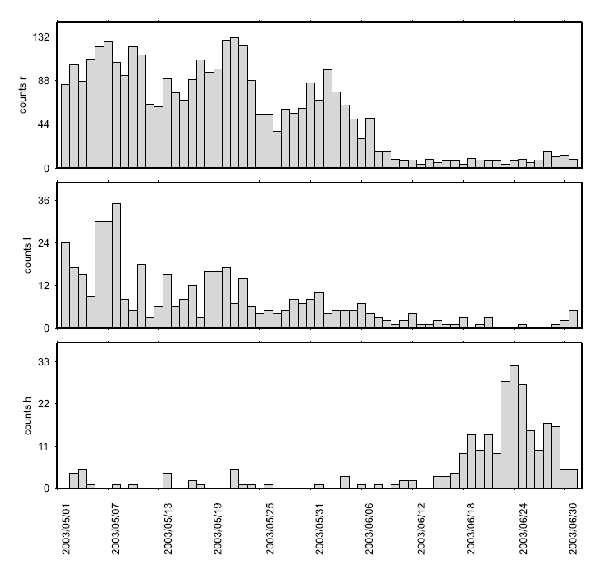
\includegraphics[width=0.9\linewidth]{fig/fig46}}
\caption{Bar diagrams showing distribution of events of different subclasses over time.}
\label{fig:volcstat}
\end{figure}

RSAM

1-minute RSAM data can be created with WAVETOOL.

Future Extensions:\newline
It is intended that additional parameters can be included in the above structure to included 
routine measurements of the volcanic earthquakes. For example, signal duration, peak amplitude 
and mean frequency can be calculated for individual stations and included on additional type 3 
lines with a volcanic identifier. Parameters on each channel can then be averaged an inserted 
on the volcanic header line.

The proposed format for these lines is as follows 

\verbatiminput{include/volc.ext}

This method of inclusion of volcanic parameters should allow for future flexibility such as incorporation of an additional parameter fields in columns 66 to 79. Also the use of type 3 lines means that existing software, such as the update program, are unaffected by these lines. 



\section{FK Analysis} 
\label{sect:fk-analysis}

The FK routines were provided by \textbf{Tormod Kv\ae rna} from NORSAR and 
implemented into SEISAN by \textbf{Andrius Pacesa}. 

\textbf{Some basics}

The FK-analysis\index{FK analysis}, more strictly slowness analysis, is a standard tool in seismic array processing\index{Array processing}. It is used to find the apparent velocity and back azimuth of an incoming wavefront. Apparent velocity can be used to identify the type of wave (P, S, Lg and etc.) and the approximate distance to the source can be determined for teleseimic events. Utilizing azimuth and distance to the source, one can define the approximate location of the signal source. 

A description of frequency-wavenumber analysis - \"f-k analysis\" - may be found in Capon (1969). This method has been further developed to include wide-band analysis and maximum-likelihood estimation techniques - see \citet{kvaerna1986}. 

The principle of slowness analysis is beamforming in the frequency domain for a number of different slowness values and calculating the power for each beam. The beam power will be a maximum in case the slowness of the beam coincides with the slowness of the wavefront crossing an array. So the beam having the maximum power will indicate the slowness of the incoming signal. 

\textbf{Running the program}

The FK program can be started directly with command `fk' or from MULPLT. The program expects that the file `waveform.out' with the seismic traces as input data, is available in the current directory. If the program is invoked directly, this file has to be created before using mulplt, selecting a window and creating the `waveform.out' file. 

In general it is more useful, to start the FK program from MULPLT since the input file needs to be created by mulplt. The result of the fk analysis can be saved to the S-file. 

The steps are: 

\begin{itemize}
\item[-]
start MULPLT 
\item[-]
select channels and a time window 
\item[-]
use option fk to start FK program (this option creates file `waveform.out' and starts FK program), 
accept maximum or pick value with mouse 

The options in FK are: \newline
\verb|                       |R-Redo: Repeat fk analysis with different parameters \newline
\verb|                       |M-Mouse: `m' or mouse click to pick values different from maximum \newline
\verb|                       |S-Save and quit: save picked value to file and quit \newline
\verb|                       |Q-Quit: quit 

\item[-]
use option `save and quit' to save your result, so that it can be used by MULPLT 
\item[-]
back in MULPLT: pick phase on the first trace used, to store back azimuth 
and apparent velocity in the S-file 
\item[-]
in case of teleseismic events, the apparent velocity can be used for location, the fk analysis has to be done on the P phase 
\end{itemize}

Note: The FK program only works by default  with station file `\texttt{STATION0.HYP}'. If coordinates are in e.g. \texttt{STATIONt.HYP}, the user will be asked to specify another station file letter, in this case `t'. 

\textbf{Example}

Input: 

\verbatiminput{include/fk.inp}

Example of output file fk.out: 

\verbatiminput{include/fk.out}

\begin{figure}
\htmlimage{scale=2.0}
\centerline{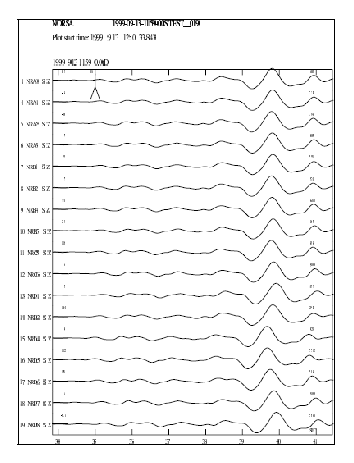
\includegraphics[width=0.9\linewidth]{fig/fig47}}
\caption{The FK program can be started from MULPLT. 
The traces shown were selected and used as input to the FK program. 
The result of the FK analysis is shown in Figure \ref{fig:fk-output}. 
The event shown here is part of the testdata set.}
%\label{fig:}
\end{figure}

\begin{figure}
\htmlimage{scale=2.0}
\centerline{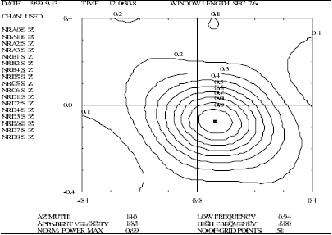
\includegraphics[width=0.9\linewidth]{fig/fig48}}
\caption{Output from the FK program. Contours and values are the normalized maximum
power.}
\label{fig:fk-output}
\end{figure}



\section{Surface wave analysis (SUN)} 

The programs by \textbf{Robert Herrmann} (Herrmann, 1996) to estimate the shear 
wave velocity of the earth by inversion of surface wave
\index{Surface wave analysis} 
group velocities
\index{inversion of surface wave group velocities} 
are distributed with Seisan. The programs are part of Herrmann's package
\index{Herrmann's package} 
``\textit{Computer Programs in Seismology}''. For more information check: 

\url{http://www.eas.slu.edu/People/RBHerrmann/ComputerPrograms.html}  

The programs have been implemented with SEISAN by Vunganai Midzi, who has written a guide on how to use the programs. This document is given as the Word file `surface.doc' in the INF directory. Also see section \ref{subs:spec} for details on output files that can be generated with MULPLT. The programs are included in the tar file `surface.tar' in the PRO directory, but are not installed as part of the standard installation. If you wish to use the programs, you need to extract the programs: 

\begin{verbatim}
cd <SEISAN_TOP>/PRO
tar xvf surface.tar 
\end{verbatim}

You can recompile the programs with the commands: 

\begin{verbatim}
make -f Makefile.sur clean
make -f Makefile.sur 
\end{verbatim}




\section{Instrument response} 
\label{sect:inst-resp}

In SEISAN the instrument response can be stored as pairs of frequency, 
amplitude and phase or as poles and zeros. The formats that can be 
used include GSE2, SEISAN, SAC and SEED. The SEISAN, SAC and GSE response formats 
are described in Appendix \ref{app:response}. For a detailed description of the GSE 
format, the reader is referred to \citet{gsett1997}. The program RESP 
creates response files in SEISAN and GSE format. SEED format response 
files can be extracted from a SEED volume.  

\subsection{Create instrument response files, RESP} 
\index{RESP}\index{Instrument response} 

\textbf{Introduction}

The purpose of this program is to (1) Make Seisan or GSE2 response files, (2) Provide the engineer maintaining seismic instrumentation with a practical tool for calculating and checking response functions of the most common elements of a seismic system. The program can calculate response functions of velocity transducers, accelerometers, filters and amplifiers, input poles and zeros or tabulated values and multiply the combinations together to get complete system response functions. The program produces a table with the response function and a simple graphical expression of the response curve. For the purpose of checking measured values, a file with these values can be used as input and will be plotted together with the theoretical values. The program can calculate, acceleration, velocity or displacement response. Program PR\_ RESP \index{PR\_RESP} can make a table of many response files. 

\textbf{The instrument response}

The seismic recording system can consist of seismic sensor, analog-digital converter, amplifier and filters. For a detailed discussion the user is referred to \citet{scherbaum1996}. The combined response can be given in the frequency domain as frequency response function or in the Laplace domain as transfer function. The frequency response is given in pairs of frequency amplitude phase (FAP), while the transfer function is given as poles and zeros (PAZ). The combined frequency response is obtained through multiplication of the response from the individual components, while the transfer function is obtained by combing the PAZ from the components. Amplifiers and accelerometers are specified simply by a constant gain. Filters are assumed to be Butterworth. RESP can be used to write finite impulse response (FIR) coefficients \citep{scherbaum1996} that are used as anti-alias filters in most modern digitizers if GSE is used as output format. SEISAN has no capability to read the FIR filters or to correct for them. However, the FIR filters are part of a full description of the instrument response and should be at least included for information if possible. 

The electrodynamic seismometer is assumed to have the following velocity frequency response: 

\begin{displaymath}
T(\omega) = \frac{\omega^{2}}{\omega_{0}^2 - \omega^2 + i 2 \omega \omega_0 h}
\end{displaymath}

which corresponds to the transfer function: 

\begin{displaymath}
T(s) = \frac{-s^{2}}{\omega_{0}^2 + s^2 + 2 s \omega_0 h}
\end{displaymath}

where $s=i\omega$, $\omega$ is the angular frequency $2\pi f$ in Hz, $\omega_0$ the 
resonance frequency of the seismometer, $i = \sqrt{-1}$ 
and $h$ the damping (normally around 0.7). 

NOTE: In the equation for the frequency response, the sign "+ 2*i*h.." was "-" before March 2000, so old parameter files may have to be regenerated.\index{Problem, RESP} The sign depends on the definition of the signs in the Fourier transform and therefore may be different  in different text books. It may even be wrong although it looks right, if a wrong Ansatz is done. Due to the wrong sign, the FAP values in the SEISAN response files were wrong, however the programs use the constants given in the files and the correct response is generated. If you have the instrument constants in your old response files and not just FAP, the old response files can be used. 

The transformation from displacement to velocity or back is done by multiplying  with i*.. 

In addition to or instead of using the equation above, values can also be entered as discrete values or as poles and zeros. 

The SEISAN response function is calculated for 60 frequencies between 0.01 and 100 Hz and the steps between the frequencies are approximately logarithmic. The response function is normalised at 
1.0 Hz ( see Table 1) and the gain at 1.0 Hz is given separately.  

NOTE: ALL UNITS ARE IN METERS, SECONDS OR G (9.8ms-2) \index{Units} 

\textbf{NOTE}: It seems that although the GSE format is clearly defined, there 
has been different interpretations. This has also led to changes in 
SEISAN since the GSE response was introduced with SEISAN. For more 
details, see Appendix \ref{app:response}. 

\textbf{Which format to use}

SEISAN, since version 7.1, supports the GSE2 calibration format in addition to the SEISAN response file format. We recommend that you use the GSE2 format, since it presents one of the most widely used calibration formats. Storage of the response in terms of PAZ is recommended over FAP, since the PAZ representation describes the continuous transfer function. You may continue using existing SEISAN response files and add new files in GSE2 format, or replace the old SEISAN response files with new GSE2 files. 

\textbf{How to run the program}

The program has quite a few options, which easily may lead to confusion. Before you start you should know which format you want to use (GSE2 or SEISAN) and whether you want to describe the response in terms of FAP or PAZ. The recommended choice is to use GSE2 and PAZ. 

Type RESP to start the program. You will then get a series of questions as indicated below in upper case letters. All input is format free. A sample run is shown below. 

CHOSE OUTPUT FORMAT: \verb|     |0: NO OUTPUT FILE \newline
\verb|                               |1: SEISAN FAP \newline
\verb|                               |2: SEISAN PAZ \newline
\verb|                               |3: GSE2 FAP \newline
\verb|                               |4: GSE2 PAZ 

Answer with 0-4, options 1-4 will create respective response files in selected format, option 0 will only calculate and show the response on the screen. SEISAN PAZ can only be used if number of poles and number of zeros are less than 38. If more are input, a table will be generated automatically in FAP format. A format with poles and zeros MUST BE USED if a mechnical displacment sensor is selectedor an accelerometer is selected which does not have first character A in component name (see later). 

TYPE OF SENSOR: \verb|      |1: NONE \newline
\verb|                         |2: SEISMOMETER \newline
\verb|                         |3: ACCELEROMETER 
\verb|                         |4: MECHANICAL DISPLACEMENT SEISMOMETER 

Answer with 1, 2, 3 or 4. Number 1 is used when only calculation of filters or amplifiers are desired, 2 is a standard velocity transduceri,  3 a standard accelerometer and 4 is a mechnical diplacement sensor (normally a digitized record of a paper seismogram). If a seismic sensor is used, you will get additional questions on the constants of the sensor. If a seismometer is chosen, the following questions must be answered: 

SEISMOMETER NATURAL PERIOD ? 

This is measured in seconds. For most short period systems the value would be 1.0 second. 

SEISMOMETER DAMPING RATIO ? 

The damping ratio should ideally be 0.7. This depends on the damping resistance. 

For both the electrodynamic seismometer and accelerometer, the following question is given: 

SENSOR LOADED GENERATOR CONSTANT (V/M/S OR V/G) ? 

This is the generator constant of the sensor in terms of volt per unit of of ground motion (meter/second or g). It is important to note that this is the loaded constant, which means the effective output of the sensor taking into account amplifier input and damping resistances.\index{Seismometer constants} 

For the mechanical sensor, the question is

 SEISMOGRAPH GAIN in TIMES GAIN (M/M) ?

which is simply the mechnical gain.

Now comes questions about amplifier, filter and recording unit. 

RECORDING MEDIA GAIN (COUNT/V OR M/V) ? 

If you have a recording media, the gain can be given here, otherwise just enter 1.0 

If the output format is GSE, the response is always calculated in displacement units, while for SEISAN output and seismometer or accelerometer, the following options appear: 

TYPE OF RESPONSE: \verb|    |1: DISPLACEMENT \newline
\verb|                         |2: VELOCITY \newline
\verb|                         |3: ACCELERATION 

Normally for a seismometer, one wants to calculate the displacement response and for an accelerometer, the acceleration response. However it might sometimes be interesting to look at e.g. 
the velocity response for a seismometer (after all, the seismometer is normally a velocity transducer !!). Enter the appropriate number. 

AMPLIFIER GAIN (DB) ? 

This is the amplifier gain in dB. Since this question is only asked once, this gain must include gain of all units except the recorder (asked below). This could e.g. include gain of the VCO system. 

NUMBER OF FILTERS (0-10), RETURN FOR NONE ? 

Up to 10 filters can be specified. If you answer 0, no filters are used and no more questions on filters will appear. Otherwise one line of input must be given for each filter as follows: 

FREQUENCY AND NUMBER OF POLES FOR EACH FILTER, \newline
POLES NEGATIVE FOR HIGH PASS 

Each line requires two numbers, the corner frequency of the filter and the number of poles. A high pass filter is given by letting number of poles be negative. It is not always easy to know whether a filter is e.g. one 2 pole or two 1 pole filters, the user needs to experiment with this. 

FILE NAME FOR FILE WITH POLES AND ZEROS, RETURN FOR NO FILE
\index{Poles and zeros}

Here a file with poles and zeros can be entered. If seismometer constants have been chosen above, the values calculated with poles and zeros are multiplied with the values previously calculated. The free format file contains: 

1. line: NP: Number of poles, NZ: Number of zeros, Norm: Normalization constant \newline
Following NP lines contain one pair each of real and imaginary poles \newline
Following NZ lines contain one pair each of real and imaginary zeros 

NOTE: The unit of frequency is radian/s so if in Hz, multiply with 
$2\pi$ and normalization constant in 
$radian = (normalization constant in Hz) 2\pi^{(number of poles-number of zeroes)}$. 

The next 2 options are only shown if the output file is selected to be FAP: 

FILE NAME FOR TABULATED VALUES, RETURN FOR NO FILE  

Here a file with tabulated values are entered. If seismometer constants or poles and zeros have been chosen above, the tabulated values will be interpolated and multiplied with the values previously calculated for from above. The free format file contains: 

1. line: N: Number of tabulated values, Norm: Normalization constant \newline
Following N lines contain one each frequancy, amplitude and phase(deg) 

GIVE FILE NAME FOR MEASURED VALUES, RETURN FOR NONE 

Give file name for measured values. In most cases you have none so just make a return. The format of the input file is as follows: 

frequency, amplitude, phase \newline
frequency, amplitude, phase \newline
etc. 

e.g. 

0.2,0.7,200 \newline
0.7,0.8,100 \newline
10.0,0.1,33 

The file has no blank lines and can contain up to 60 data sets. It is important to note that the amplitude values should be NORMALIZED at 1.0 Hz. 

Now there is no more input to the response parameters, and the output is: 

GAIN FACTOR AT 1.0 HZ: 12345.6 

This is the gain of the system at 1.0 Hz and is also the value for normalizing the response curve, that is, all calculated values are divided by this number. There is no unit for gain of an amplifier and for displacement response using a seismometer and drum recording. If the recording is digital, the unit would be counts/meter and for a velocity response counts/meter/second etc. If a file with poles and zeros is used without any other information, the \index{Normalization constant}normalization constant must have the unit of count/m, similar for the tabulated input. 

Further output is given in a file called resp.out, see Table 1 for an example. 

The response curves (amplitude and phase) are now printed/plotted on the screen. First comes the amplitude response (amplitude in db versus log frequency). By pushing return, the phase response is shown (phase shift (deg) versus log frequency). After the plots, the SEISAN \index{Calibration file}calibration file can optionally be made, follow instructions, see example below. The response file MUST be calculated for the displacement response, and all calculation in SEISAN assume that response is calculated in counts/m. 

After the SEISAN response file is made, the current parameters will be displayed and one or several can be changed without entering all again. Like if the gain has changed at a certain date, only change date and gain. This feature (new in SEISAN7.2) has been put in to be able to quickly make many similar response files, like when all files have to be put in for a network. 

\textbf{Comments to data for response files}

\index{Station and channel codes}
Station and channel codes \newline
It is important that the station and channel codes are made exactly as they appear in the waveform files. If not, SEISAN is not able to identify the channel. 

Date \newline
The date given here corresponds to the date from which the calibration information is valid. The SEISAN system will always look for the most recent calibration file relative to the date of the earthquake. 

Latitude, longitude and elevation \newline
These data are for information only, it is not used anywhere in 
SEISAN, so it does not have to be entered, however there is room for 
it in the SEISAN waveform file headers. 

Comment \newline
No information used by the system. 

Plot \newline
After the response file has been written out, a plot is made 
with PRESP of the file. There will also be a plotfile, 
\index{Presp.eps}
\texttt{presp.eps}, which can be sent to the printer. 
The response file can store the response in different ways: 

\begin{enumerate}
\item
Parameters used for calculating the response: Generator constant, filters etc. In addition, the response (amplitude and phase) at 30 frequencies are listed. In this case the response is calculated from the parameters. 
\item
Incomplete set of parameters or no parameters and the response at 30 frequencies. In this case the response is calculated by interpolation of the 30 values. 
\item
Poles and zeros: No discrete values are given and the response is calculated directly from the poles and zeros. 
\end{enumerate}

See also Appendix \ref{app:seisan-format} for the SEISAN 
waveform file format and section \ref{sect:system-response}. 

\textbf{IMPORTANT: PUT RESPONSE FILE IN CAL DIRECTORY OR ONE OF ITS STATION SUBDIRECTORIES. Response files can also be in working directory but this is not advisable except for testing.}

\textbf{Example of running the program:}

\verbatiminput{include/resp.run}

\index{Problem: Response file naming} 
\textit{\textbf{Problem: The response file naming has not changed according to the SEED convention so location and network code cannot be entered using RESP, however they can be entered manually in response file (see response file format). This menas that e.g. SHZ must be entered as SH Z since only 3 of the 4 character are used. For older data in SEISAN format, all 4 characters can be used.}}

Examples of response files is given in Appendix \ref{app:response}.

\subsection{Examples of main response files from seismometers and accelerometer} 

Example of a G\"uralp DM 24 digitizer with CMG-40-1 (1 Hz) 

\textbf{Digitizer:}

The sensitivity of the digitizer is given to $3.197 \mu V/count$. The SEISAN gain is in counts/V so 

SEISAN recording media gain =1000000/3.197 = 312793 count/V 

\textbf{Sensor:}

Sensitivity is 2 X 1001 V/m/s =2002 V/m/s 

\textbf{Making response file with parameters}

For calculating with parameters, it is assumed that the free period is 1.0 s and damping is 0.7. Using the resp program answering as follows 

Output format: 0 \verb|                | Only testing \newline
Type of sensor: 1 \verb|                | It is a seismometer \newline
Seismometer period: 1.0 \newline
Seismometer damping: 0.7 \newline
Generator constant: 2002 \newline
Recording media gain: 312793 \newline
Amplifier gain: 0  \verb|                |  No amplifier \newline
Number of filters: enter \verb|                | No filter \newline
File with poles and zeroes: enter \verb|                | We use parameters now \newline
File with tabulated values: enter \newline
File with measured values enter 

Then the plot below comes up 

\begin{figure}
\htmlimage{scale=2.0}
\centerline{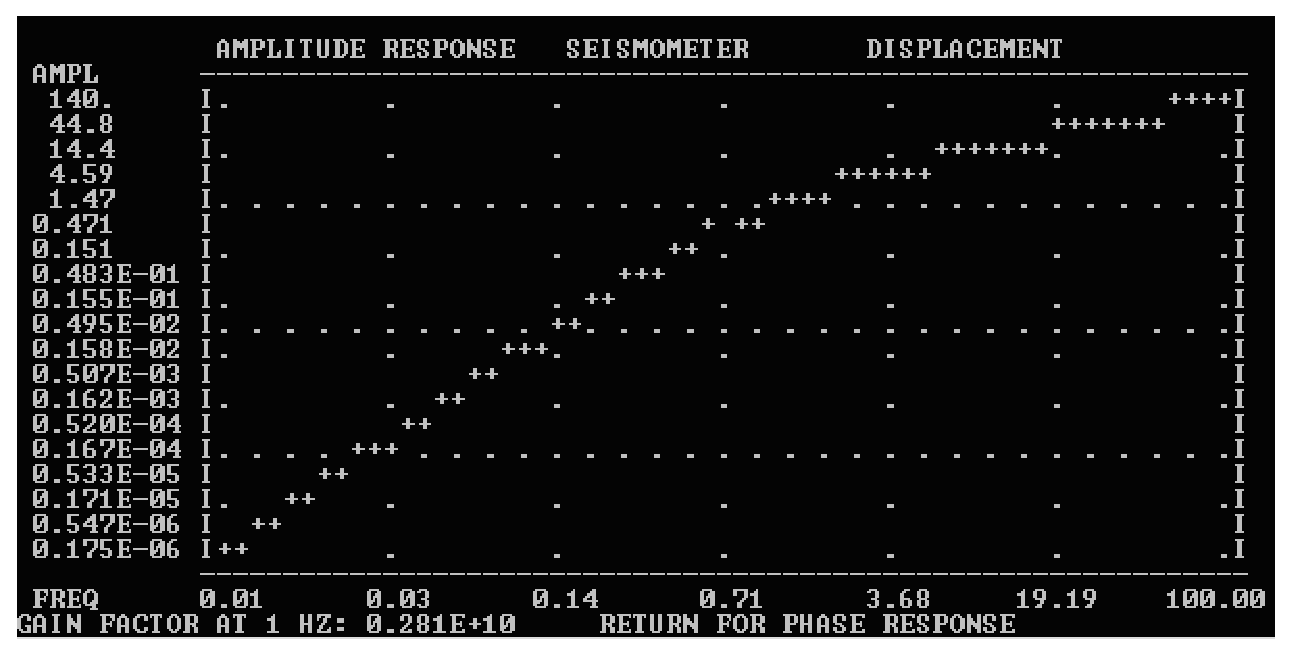
\includegraphics[width=0.9\linewidth]{fig/fig49}}
\caption{Making response file with parameters.}
%\label{fig:}
\end{figure}

\textbf{Making response file with poles and zeros}

The poles and zeroes velocity response in units of Hz is given as 

Poles \newline
-0.707 0.707 \newline
-0.707 -0.707 \newline
-62.4 135.4 \newline
-62.4 -135.4 \newline
-350.0 0.0 \newline
-75.0 0.0 

Zeros \newline
0.0 0.0 \newline
0.0 0.0 

SEISAN units are radians/sec so poles and zero values  are multiplied by $2\pi$. \newline
The normalization constant is given as $585.8 10^{6}$. To convert to radian is done as follows 

Normalization constant in radian = $585.8 10^{6} (2\pi)^{(number of poles-number of zeroes)} 
= 585.8 10^{6} (2\pi)^{4} = 9.12 10^{11}$. 

SEISAN also uses displacement so one zero is added. The values are then 

Poles\newline
-4.442 4.442 \newline
-4.442 -4.442 \newline
-392.0 850.7 \newline
-392.0 -850.7 \newline
-2199.0 0.0 \newline
-475.0 0.0 

Zeros \newline
0.0 0.0 \newline
0.0 0.0 \newline
0.0 0.0 

To get total constant (gain and normalization constant),  we multiply by sensor gain and digitizer gain 

Total normalization constant = $9.12 10^{11} x 2002 x 312793 = 5.71 10^{20}$ 

A SEISAN input file is then made 

6 3 5.71e20 6 poles, 3 zeros and total gain constant \newline
-4.442 4.442 \newline
-4.442 -4.442 \newline
-392.0 850.7 \newline
-392.0 -850.7 \newline
-2199.0 0.0 \newline
-475.0 0.0 \newline
0.0 0.0 \newline
0.0 0.0 \newline
0.0 0.0 

The resp program now makes the SEISAN response file with this input as follows 

Output format: 0 Only testing \newline
Type of sensor: 0 Sensor response is in poles and zero file \newline
Recording media gain: 1 Gain has been put into total gain constant \newline
Amplifier gain: 0   No amplifier \newline
Number of filters: enter No filter \newline
File with poles and zeroes: \texttt{resp.inp} File with poles and zeros, can be any name \newline
File with tabulated values: enter \newline
File with measured values enter 

Then the plot below comes up 


\begin{figure}
\htmlimage{scale=2.0}
\centerline{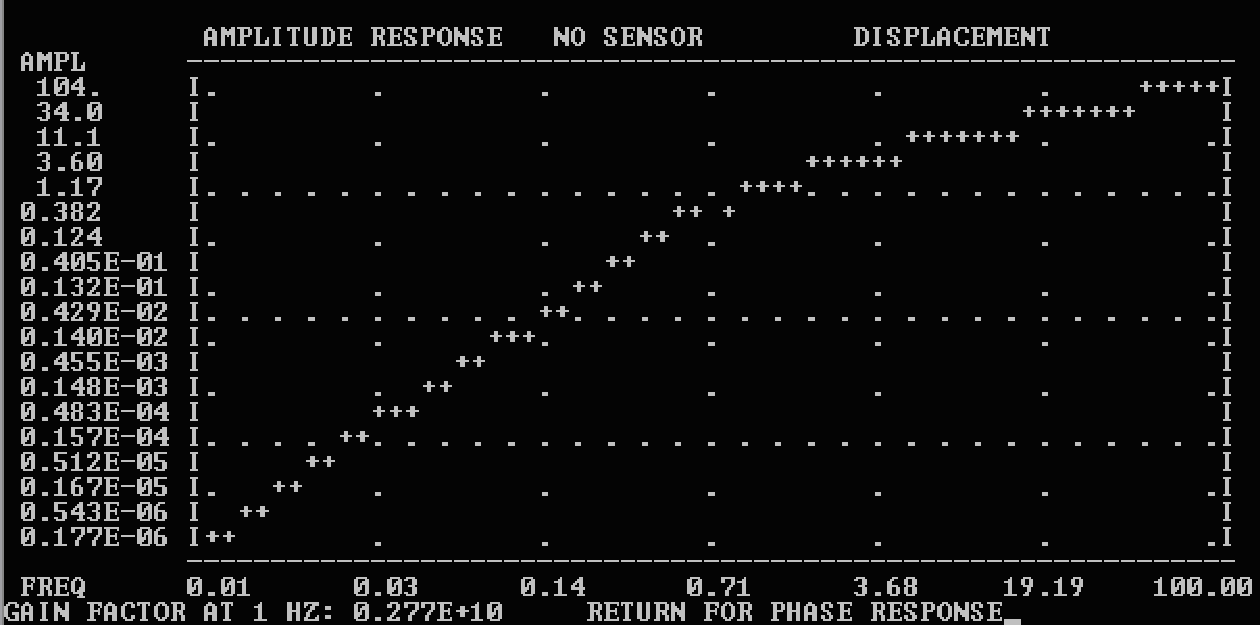
\includegraphics[width=0.9\linewidth]{fig/fig50}}
\caption{Making response file with poles and zeros.}
%\label{fig:}
\end{figure}

It is seen that the two ways of making the response file gives almost the same result, however using poles and zeroes is the most accurate, particularly for active sensors. In both cases no consideration was made for antialias filters which normally can be disregarded if a modern sharp filter. 

\textbf{Example of a Gurlp DM 24 digitizer with CMG-5T accelerometer}

The digitizer is the same as before 

Using parameter format, SEISAN currently requires the component name to start with A. According to international standards, the component code for an accelerometer should be something like ENZ so a parameter format cannot be used and poles and zeroes must be used. For the CMG-5T, the only information about the sensor is the sensitivity of 1V is equivalent to 0.970 m/s2 1.03 V/ms-1. In SEISAN parameter format this should be converted to V/g so sensitivity is then 

9.81 (ms-2/g)/0.97(ms-2/V) = 10.1 V/g  

\textbf{Parameter format}

The input is:  

Output format: 0  Only testing  \newline
Type of sensor: 3  It is an accelerometer  \newline
Generator constant: 10.1  \newline
Recording media gain: 312793  \newline
Amplifier gain: 0   No amplifier \newline
Number of filters: enter No filter \newline
File with poles and zeroes: enter We use parameters now \newline
File with tabulated values: enter \newline
File with measured values enter 

The plot below comes up 

\begin{figure}
\htmlimage{scale=2.0}
\centerline{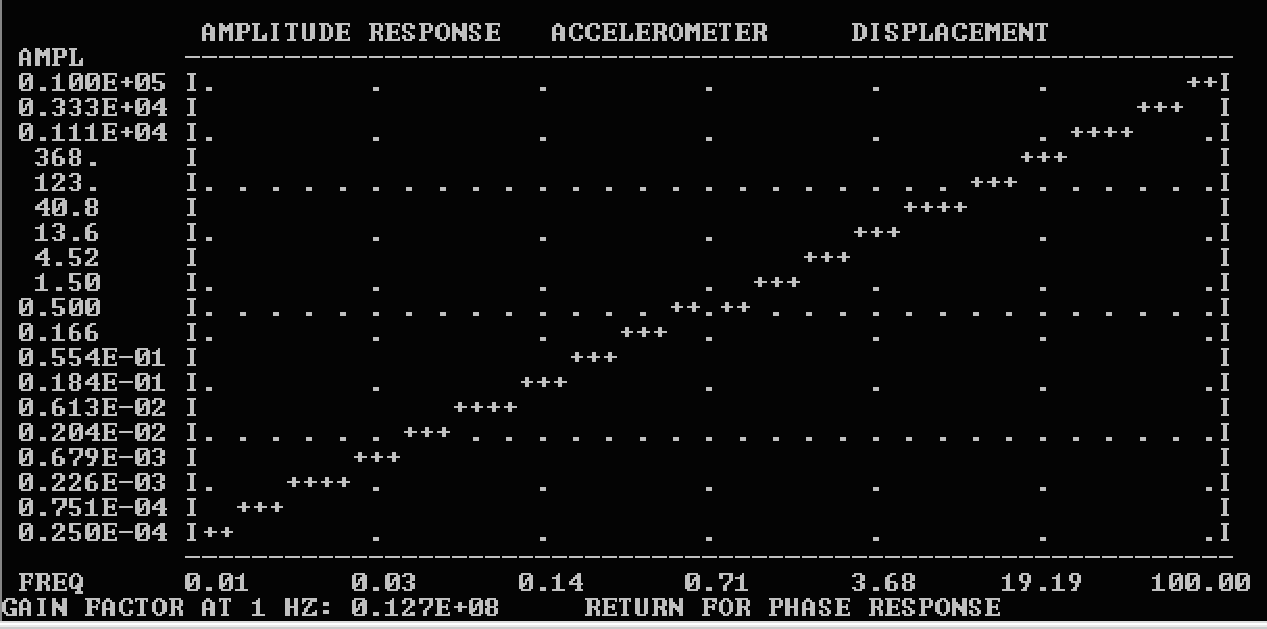
\includegraphics[width=0.9\linewidth]{fig/fig51}}
\caption{Making response file for an accelerometer woth parameters.}
%\label{fig:}
\end{figure}

\textbf{Poles and zeros}

The displacement response for an accelerometer consists of 2 zeros 
and normalizarion constant of 1. The total gain constant is then 

312793 x 1.03 = 322000 

So the input file for resp is 

0 2 322000\newline
0 0 \newline
0 0 

The manual input is exactly as above in the other example of using a poles and zero input file and the output is exactly as for the example of using parameter input. 

\textbf{Making a response file for a particular station}

For a particular station, chose output format SEISAN PAZ or GSE2 PAZ 
and later answering yes to question of making the SEISAN response 
file (see SEISAN manual ???????????????). 
If e.g. the station has station code TEST and component name S Z, 
the a response file valid from January 1, 2007 will have the name 
\texttt{TEST\_S\_\_Z.2007-01-00-0000\_SEI}. 
In case of a SEISAN poles and zero file, the content is:  

\verbatiminput{include/resp.sei}

So the file could have been made without using resp. 

Table 1 Example of \texttt{resp.out}: 

\verbatiminput{include/resp.out}

FOR MORE DETAILS ON HOW TO UNDERSTAND GSE AND SEED RESPONSE PARAMETERS, 
SEE \citep{havskov2004}, chapter 6. 

\subsection{SEED response} 


SEISAN can directly read SEED responses, which is poles and zeros, 
given as velocity response and transfer function types A (Laplace 
Transform in Rad/sec) and B (Analogue in 1/sec). Storage of response 
in one of these is the most common. The resp files can be created 
with rdseed from a full or dataless SEED volume 
(\texttt{rdseed -R -f seed\_volume}). RDSEED creates files with the 
pattern texttt{RESP.NC.STAT.LC.CHC}, where \texttt{NC}=network code, \texttt{STAT}=station code, 
\texttt{LC}=location code (not used by SEISAN) and \texttt{CHC}=channel code. The resp 
files need to be stored in the CAL directory and SEISAN will find 
the correct file. The resp file can contain response information from 
several time intervals. SEISAN uses the date and time of the waveform 
data to find the corresponding instrument response. 

SEED response files are given in stages, for example seismometer, digitizer and FIR filters are stored as individual stages. The overall response is made by combining all the stages. SEISAN uses the following blockets from the SEED resp file (for more details see \citet{iris1993}):

B052F22 - start date \newline
B052F23 - end date 

B053F03 - transfer function type, A=Laplace Transform (Rad/sec), B=Analog (1/sec) 

B053F07 - A0 normalization factor (A0 is checked against poles and zeros at normalization frequency and changed if not correct). The product of poles and zeros at the normalization frequency and A0 gives 1. 

B053F08 - Normalization frequency 

B053F10-13 - zeros, if transfer function type is B, normalization factor A0 is changed to (A0)/(2 pi) for each zero 

B053F15-18 - poles, if transfer function type is B, normalization factor A0 is changed to (A0)*(2 pi) for each pole 

B058F04 - gain 

The overall gain factor is given by the product of normalization factors and gain factors from all stages. One zero is added to convert to displacement response. It is assumed that input units are V/m and output units are counts, no checks are done on input and output units. 

\subsection{SEED response to GSE, SEEDRESP2GSE} 

SEEDRESP2GSE converts SEED resp files as written out by rdseed to GSE format. The program only supports poles and zeroes and transfer function type Laplace Transform. The program asks for station and component names and a time. This is because the resp file could have data from several channels and cover several time intervals with different instrument configuration. 

\subsection{GSE response to SEED, GSERESP2SEED} 

GSERESP2SEED can be used to build dataless SEED volumes from a set of 
GSE calibration files. The conversion is based on the GSE2SEED 
program by \textbf{Reinould Sleeman} (email sleeman@knmi.nl). Input can 
be single filenames or a list of files given in \texttt{filenr.lis}. The program produces a single channel SEED volume for each channel given by a GSE response file. At the end of the output filename, GSE is replaced by SEED. Other tools have to be used to merge several channels into one SEED volume. If there are several GSE files for a channel from different time periods, a stop date has to be given in the CAL2 line of the respective GSE file. Station coordinates are taken from the \texttt{STATION0.HYP} file. The program can use the site name, if it is part of the GSE response file through a comment line as in the following example: 

\begin{verbatim}
 (GSE2SEED_SITENAME Charnwood Forest, Leicestershire, England, UK) 
\end{verbatim}



\section{Macroseismic data in SEISAN} 
\label{sect:macro}

\index{Macroseismic information}\index{Felt information} Macrocosmic information in SEISAN are of 2 kinds. The summary information with maximum intensity, macroseismic epicenter etc has a special line in the S-file (see Appendix1) and the SELECT program can search for felt events. In addition, from SEISAN, version 8.1, a format has been defined to store macroseismic observations used to create e.g. maps with isoseismals. The observations files are stored in a local ISO format. For a format description and suggestion for file names, see Appendix \ref{app:nordic}.
There are currently no SEISAN programs that generates these files so they have to be made manually from the observations. The files in ISO are linked to the events as given by the S-file data base structure in the same way as waveform files are linked to the events. The line type is MACRO3 and an example is 

\begin{small}
\begin{verbatim}
 2007-01-21-1345-00.MACRO                                            MACRO3 
\end{verbatim}
\end{small}

Thus information about event source parameters and felt information is available together. An 
example of a file is  

\verbatiminput{include/macro.fil}

The file format is given in Appendix \ref{app:nordic}. Program EPIMAP can plot the new files (use  macroseismic file instead of a hypocenter file). The requirement is that the the first 3 letters after the `.' is mac or MAC (as example above). The intensities will be plotted as number on the map. A new Unix program can also be used with the data. Program \index{MACROMAP}MACROMAP can use the macroseismic observation file as input to create a map of the observations using GMT. The program generates a GMT script file, macromap.gmt, which then is executed from within the program to create a PostScript output file, \index{Macromap.ps} macromap.ps. This file is then displayed, from within the program, with Unix command gv (GhostView).
%\textcolor{red}{jh-change:
The program also runs under Windows, but does not plot. 

The input can also be from a file made with macroquest (web based interactive program for input from the public, to be distributed with SEISAN CD). In addition to making the plot, a conversion from the web format to SEISAN format is made (output file macromap.out). This option requires an input file with postal codes in order to get location of the observations. 
MACROMAP can also be executed directly or from eev. When executed directly from the prompt line, the options are: 
-macroinput file with macroseismic observations, SEISAN format, abs path or in ISO -placename optional additional file with place names, to be shown on map, abs path or in DAT,  
                         epimap format is used -postfile optional file with postal code, abs path, used with web option  
If used with eev, the place name file must have name place\_names.macro \index{Postal code } 

\begin{figure}
\htmlimage{scale=2.0}
\centerline{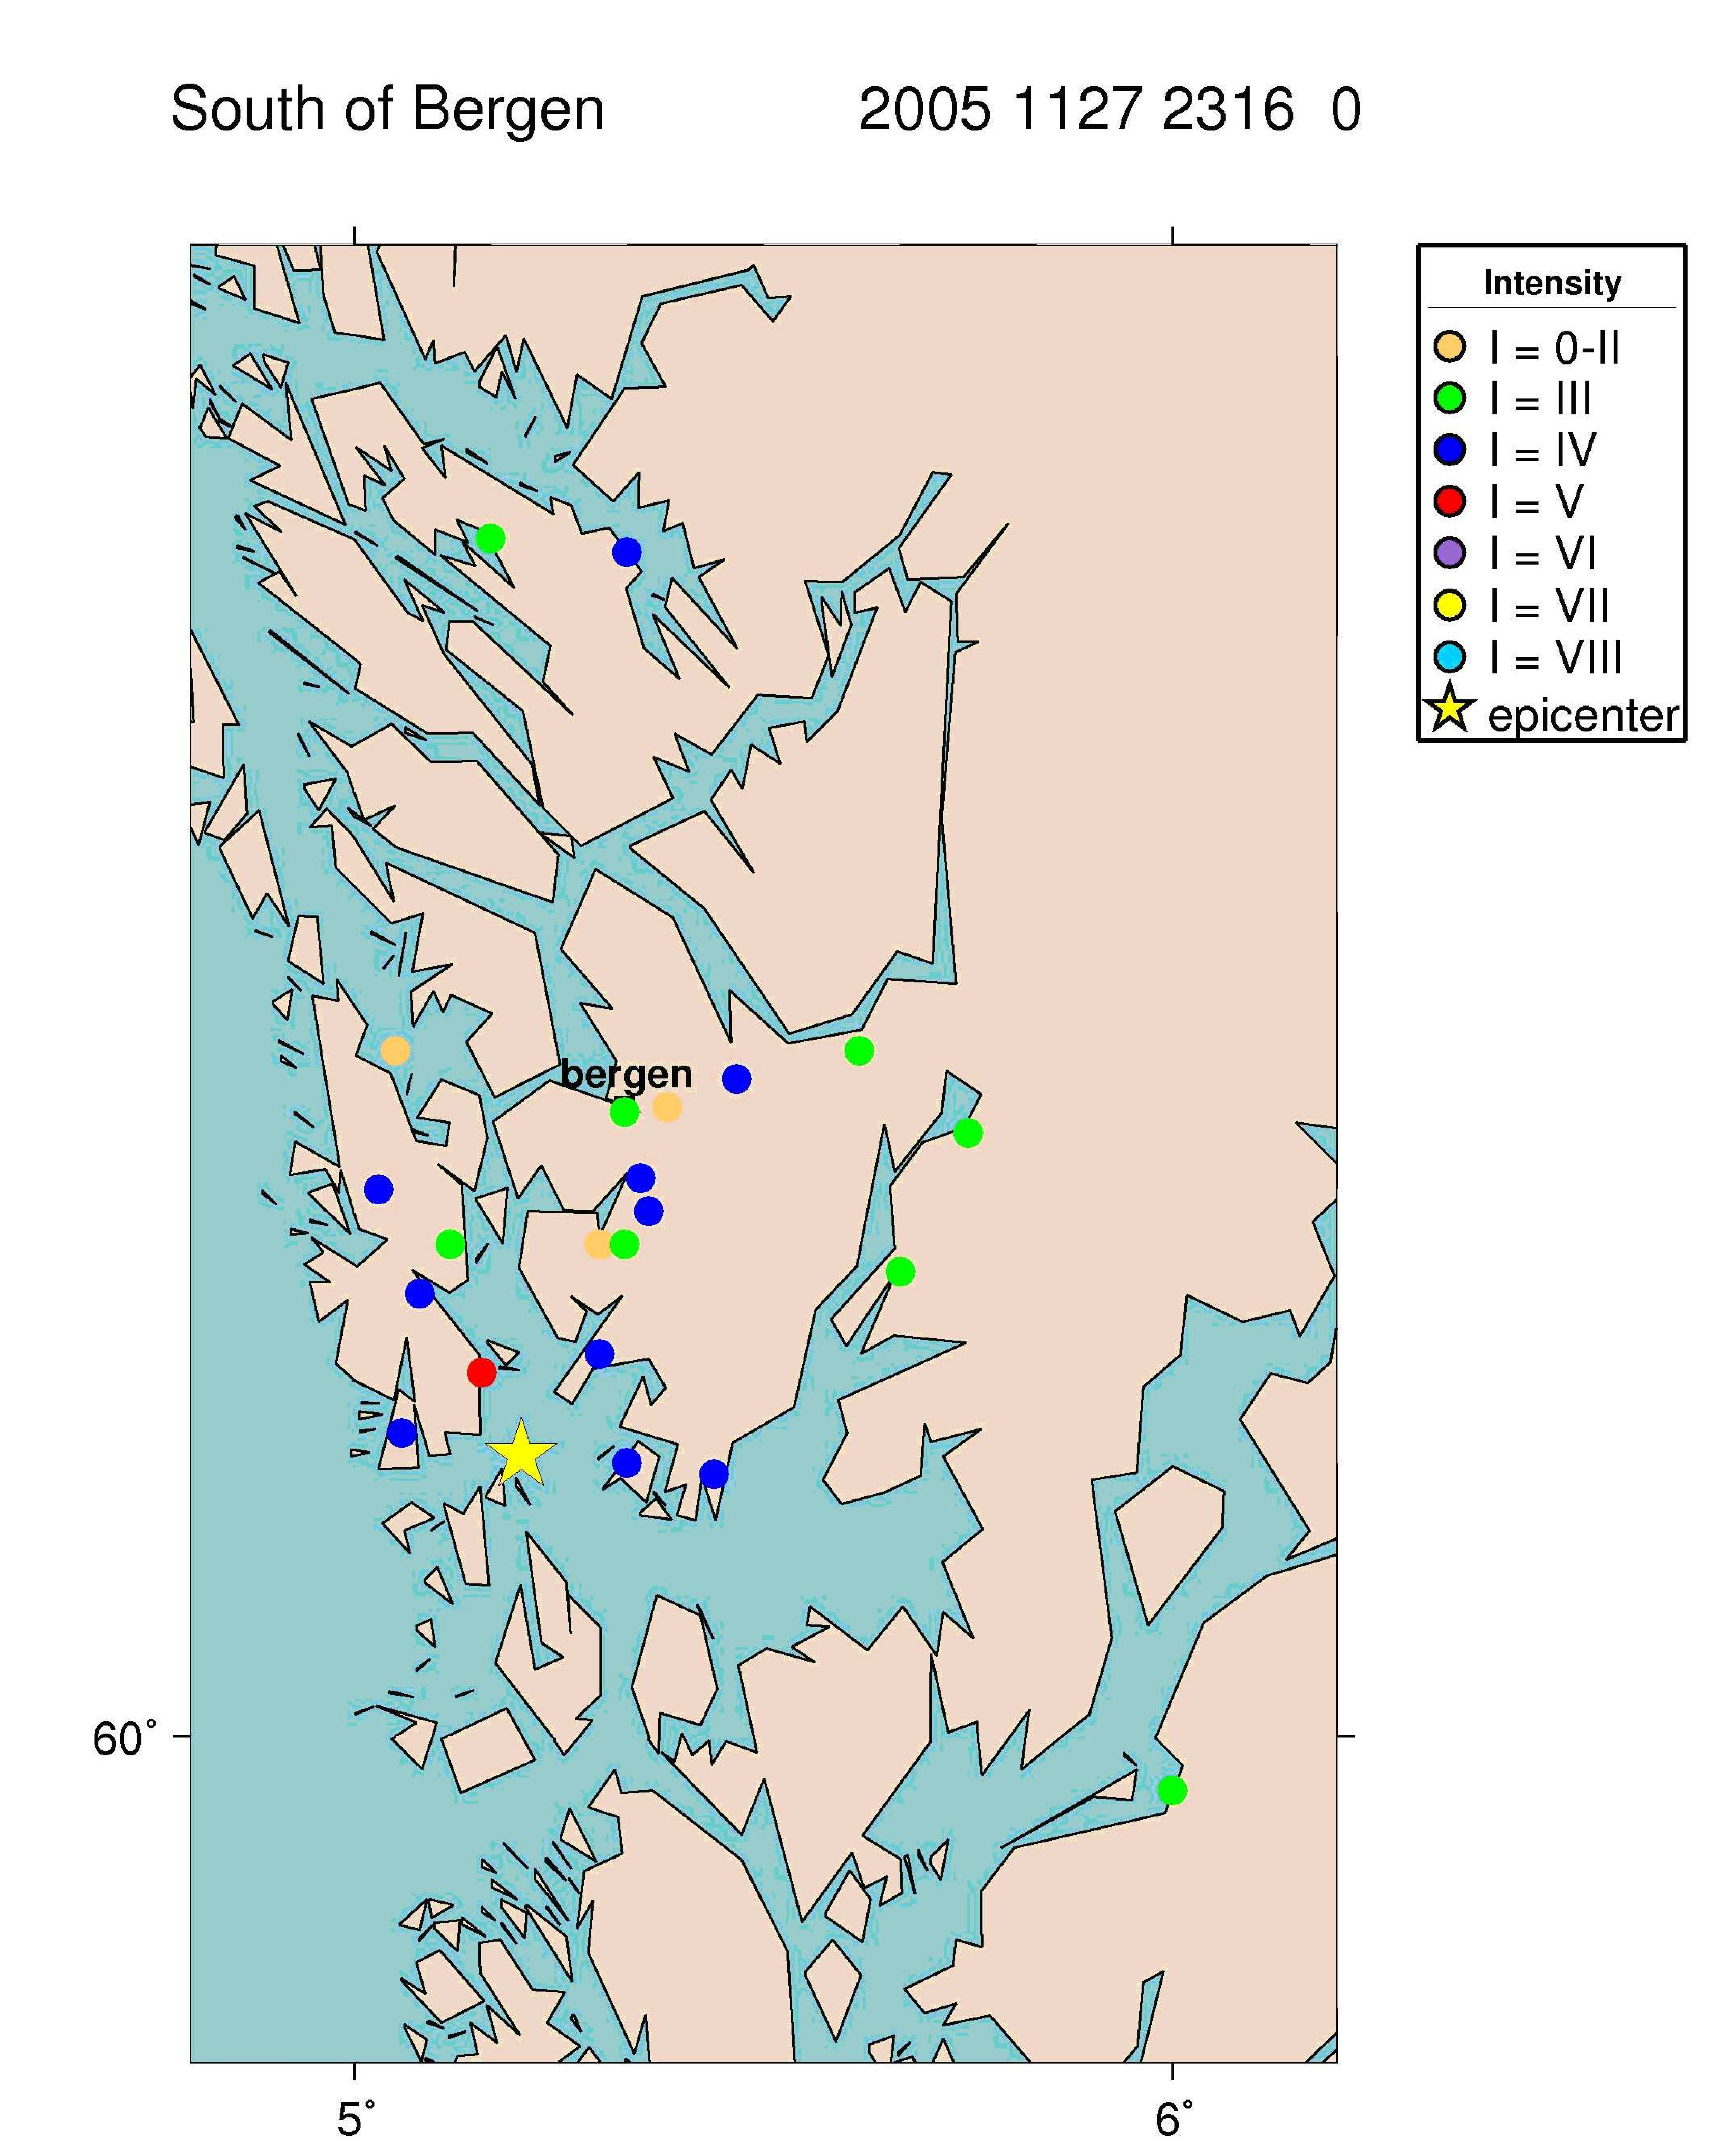
\includegraphics[width=0.9\linewidth]{fig/fig52}}
\caption{Macroseismic map made with MACROMAP using EEV. 
The epicenter, taken from the S-file, is shown with the star.}
%\label{fig:}
\end{figure}

An example of the postal code file is 

\verbatiminput{include/macro.fil}

The content is postal code, latitude, longitude and location. The format is a10,ff10.3,2x,a30. the postal code does not have to be a number, but can be any string. 



\section{Correlation of waveform signals, CORR and detection of event clusters XCLUST}

\index{Correlation}\index{CORR}\index{XCLUST} 
The cross-correlation function provides a measure of similarity between signals. 
In seismology cross-correlation can be used to measure the similarity 
of waveforms between seismic events and in case of similarity to determine relative arrival times of a seismic wave between two events. Waveform similarity is caused by proximity in hypocenter location and similarity in focal mechanism between two events. Cross correlation can be computed with the program CORR and the output be processed with program XCLUST to detect groups of similar events. 

\textbf{CORR}

The program CORR computes correlation and can be used to measure relative arrival times. It also can be used to determine correlation of a master event with continuous data and extract event based data. The output of maximum correlation for a station recording different events can be used to identify event clusters within the data set, this can be done using the program XCLUST.  
The cross-correlation function of signals x and y is computed in the time domain as: 

\begin{displaymath}
r_{xy}(i) = \frac{\sum_{j=1}^{n} x_j y_{(j+i-1)}}
{\sqrt{\sum_{j=1}^{n} x_j^2} \sqrt{\sum_{j=1}^{n} y_{j+i-1}^2}}
\end{displaymath}

Phase arrivals 

Phase arrivals of similar events can be determined accurately through cross-correlation. P and S arrivals can be determined independently. The procedure starts by selecting and picking phases for a master event that is representative for the group of events. Analysis of this event needs to be done accurately as it is the basis for the subsequent analysis. Phases of the other events in the group can be determined through cross-correlation of either the complete trace or a selected phase window with the master event. To pre-select a time window, manual identification of the phase for subsequent events is required prior to running CORR. This may be necessary for example if the waveform file contains several events. The phase arrival time is given by the maximum of the cross-correlation function that needs to exceed a minimum threshold. The arrival time is written out as absolute time. Filtering is applied to the signals if selected for both master and subsequent events, this may be necessary especially when dealing with events of different size. The filtering introduces a phase shift, which is applied to both signals. However, the absolute phase arrival for the subsequent event is consistent with the master event picked time. 

The calculation of the relative phase time (dt) is done by taking 
the travel time for the master event (AT1 -OT1) (where AT is arrival time and OT origin time) minus the travel time of the other event (CAT -OT2), where CAT is the time corresponding to the maximum amplitude in the cross correlation function. The output file dt.cc can be used with the double difference location program HYPODD. \index{HYPODD} 

Cross correlation matrix

In this mode the cross-correlation is computed between the same stations for all pairs of events (that fulfill the criteria for maximum distance between the events, and event and station). The resulting 
cross-correlation matrix (for each station containing $\sum_{i}^{n}(i-1)$ values, where n is the number of 
events) can be used to identify groups of similar events using the program XCLUST.  

Continuous mode 

The main objective of running CORR in this mode is to identify a master waveform signal in a continuous data stream, given by waveform data files. The times when correlation is higher than the selected threshold level are written out, and can be visualized by splitting the corr.out file and using EEV and MULPLT. In addition, it is possible to cut out individual event files (see CONTINUOUS EXTRACT parameter). 

Input file 

Input to the program is given through the file corr.inp. A sample file is given in the DAT directory; the data used in the example are part of the test data set (TEST database 2003/06, see training document). The program is run by command corr in the same directory as corr.inp and the s-files. The waveform files can be in any SEISAN standard place. All standard waveform formats can be used. 

The parameters in \texttt{corr.inp} are as follows:

Event file names: 

\begin{tabular}{lp{11.0cm}}
SFILE MASTER: & sfile name of master event, remove or comment out this parameter 
                to run program in group identification mode to determine 
                cross-correlation matrix between all events and identify group of similar events \\
SFILE EVENT:  & sfile name of events that will be either cross-correlated among themselves, or 
                compared to the master event, there can be several of these. \\
SFILE INDEXFILE: & texttt{filenr.lis} file can be used to give S-file names instead of listing 
                   them with `SFILE EVENT' \\
\end{tabular}

General parameters: 

\begin{tabular}{lp{8.0cm}}
INTERACTIVE: & set to 1. for interactive use where graphics are 
               displayed on the screen, which is useful for testing; 
               or set to 0. for non-interactive run \\
CC MATRIX WINDOW: & time interval in seconds to use in computation of cross-correlation matrix instead of the duration given for each station given on STATION line, if different from 0.; full trace is used if EVENT SELCRIT is set to 0. \\
CONTINUOUS MODE: & write out all detection times for correlation above threshold if set to 1.; otherwise only phase for maximum correlation CONTINUOUS EXTRACT: extract event waveform files for correlation above threshold, 0. for no extract, 1. to extract single channel used, 2. extract all channels  \\
EVENT SELCRIT: & cross-correlation with the master signal can be computed either for the complete trace of the subsequent event (0.) or the same part of the signal (either P or S) as for the master event (1.) including the pre signal part and of the same duration as defined in STATION line \\
FILTER: & this parameter allows to enable (1.) or disable (0.) filtering as defined for each channel with parameter line \\
STATION FIX DEPTH: & allows to fix depth to given value in corr.out, which 
                    can be useful if data is input to 
                    location program; set to 999. to disable \\
MAX EVENT DISTANCE: & maximum distance between event pair to compute correlation \\
MAX STAT DISTANCE: & maximum distance between event and station \\
MIN CORR:&  minimum correlation required either for grouping or phase identification \\
MIN CORR CHAN: & number of stations required for event pair to be correlated. \\
N DOUBLE SRATE: & if sampling rate is to be increased give factor n to double sampling rate n times, 
0. for none, this makes it possible to get phase reading with resolution greater than 
sampling interval \\
PRE SIGNAL: & duration of signal to include before phase arrival if used \\
SINGLE BIT: & the data can be reduced to 1 bit; reduce to 0 (-) and 1 (+) if set to 1, full data if set to 0.  \\
START LATITUDE and START LONGITUDE: & these can be set to write values to corr.out, which is in 
Nordic format and can be used as input for location programs; this can be used if all events analyzed belong to one cluster and the same starting location is to be used for all of them; set to 999. to disable \\
TRACE OUTPUT: & flag to write corr.trace output file (1. for true) \\
WAVE CORR OUT: & CORR can write out cross-correlation function and input traces to waveform output files of the selected duration, to disable set this parameter to 0., 1. for full data or 2. for reduced data, where 1 for data > MIN CORRELATION, otherwise 0 \\
WAVENAME OUT: & CORR writes out waveform filenames to corr.out, it is possible to either keep original waveform names (0.) or put corr output file names (1.), which after SPLIT of corr.,out allows inspection of the results using eev and mulplt  \\
\end{tabular}

Station parameters: 

\begin{tabular}{lp{11.0cm}}
STATION: & one line for configuration of each channel 
\begin{tabular}{lp{7.0cm}}
STAT, COMP: & station and component codes \\
SELCRIT: & 1=P, 2=S, 4=full trace \\
DURATION: & signal duration in seconds if (selcrit<4) starting from either P or S \\
FLOW, FHIGH: & filter limits for bandpass filter, can be; can be disabled by FILTER (see above)  \\
\end{tabular}
\end{tabular}

Example of STATION line: 

\verbatiminput{include/corr.stat}

Output files: 

\texttt{corr.out}: This is the main output file. The file is in Nordic format and contains the phase readings if run in phase detection mode and can be used with the SEISAN location programs directly. In continuous mode, the file can contain more than one phase reading per channel. In group identification mode the file contains the event list, cross-correlation matrix and suggested groups of similar events. \newline
\texttt{corr.trace}: This files gives details of program run and can provide information on cause of errors. dt.cc: Input file for hypodd giving relative phase times and correlation (see hypodd manual for details), 
e.g. \newline
\verbatiminput{include/corr.trace}

\texttt{cc\_pairs.out}: List of event pairs giving, index and s-file of first event, index and s-file of second event, number of stations and average correlation of all stations. This file is used as input to XCLUST. 

\verbatiminput{include/cc_pairs.out}

\textbf{XCLUST}

XCLUST is a simple program for cluster analysis of output from program 
CORR (\texttt{cc\_pairs.out}) to identify groups of similar events. 
This is done in a rather simple approach: 

\begin{itemize}
\item
sort event pairs with descending correlation 
\item find group 
\begin{itemize}
\item[o]start with highest correlation 
\item[o]
add events that are linked into group this group in several loops over all pairs until no more events can be added to group; link into group is given by one of the events in the pair being correlated with any of the events in the cluster 
\end{itemize}
\item continue to find next group 
\end{itemize}

Visual inspection of the waveforms is highly recommended to confirm the clustering results. 

Input file: \texttt{xclust.par}

This is the file for the main parameters, which are: \newline
MINIMUM CORRELATION: minimum correlation required for pair to be used \newline
MINIMUM STATIONS: minimum number of correlated stations required for pair to be used \newline
MINIMUM PERGROUP: minimum number of events required to make a group \newline
TRACE OUTPUT; flag to write trace output file (1. for true) 

Output files: 

\texttt{xclust.trace}: gives some details of what the program does, useful for debugging \newline
\texttt{xclust.out}: gives list of events for each cluster and for each event the number of links with other events in that cluster 

\begin{verbatim}
============= 
 group:     1 number of events:      20 
-------------
  event links 
-------------
      5     7 
     11     8 
      6     5 
      2     7 
      1     6 
      7     9 
...
\end{verbatim}

\texttt{Index.xxx}: Index file where xxx refers to number of cluster. This file 
can be used with eev (e.g. \texttt{eev index.001}) to work on a specific cluster. 



